% Options for packages loaded elsewhere
\PassOptionsToPackage{unicode}{hyperref}
\PassOptionsToPackage{hyphens}{url}
%
\documentclass[
]{book}
\usepackage{amsmath,amssymb}
\usepackage{iftex}
\ifPDFTeX
  \usepackage[T1]{fontenc}
  \usepackage[utf8]{inputenc}
  \usepackage{textcomp} % provide euro and other symbols
\else % if luatex or xetex
  \usepackage{unicode-math} % this also loads fontspec
  \defaultfontfeatures{Scale=MatchLowercase}
  \defaultfontfeatures[\rmfamily]{Ligatures=TeX,Scale=1}
\fi
\usepackage{lmodern}
\ifPDFTeX\else
  % xetex/luatex font selection
\fi
% Use upquote if available, for straight quotes in verbatim environments
\IfFileExists{upquote.sty}{\usepackage{upquote}}{}
\IfFileExists{microtype.sty}{% use microtype if available
  \usepackage[]{microtype}
  \UseMicrotypeSet[protrusion]{basicmath} % disable protrusion for tt fonts
}{}
\makeatletter
\@ifundefined{KOMAClassName}{% if non-KOMA class
  \IfFileExists{parskip.sty}{%
    \usepackage{parskip}
  }{% else
    \setlength{\parindent}{0pt}
    \setlength{\parskip}{6pt plus 2pt minus 1pt}}
}{% if KOMA class
  \KOMAoptions{parskip=half}}
\makeatother
\usepackage{xcolor}
\usepackage{color}
\usepackage{fancyvrb}
\newcommand{\VerbBar}{|}
\newcommand{\VERB}{\Verb[commandchars=\\\{\}]}
\DefineVerbatimEnvironment{Highlighting}{Verbatim}{commandchars=\\\{\}}
% Add ',fontsize=\small' for more characters per line
\usepackage{framed}
\definecolor{shadecolor}{RGB}{248,248,248}
\newenvironment{Shaded}{\begin{snugshade}}{\end{snugshade}}
\newcommand{\AlertTok}[1]{\textcolor[rgb]{0.94,0.16,0.16}{#1}}
\newcommand{\AnnotationTok}[1]{\textcolor[rgb]{0.56,0.35,0.01}{\textbf{\textit{#1}}}}
\newcommand{\AttributeTok}[1]{\textcolor[rgb]{0.13,0.29,0.53}{#1}}
\newcommand{\BaseNTok}[1]{\textcolor[rgb]{0.00,0.00,0.81}{#1}}
\newcommand{\BuiltInTok}[1]{#1}
\newcommand{\CharTok}[1]{\textcolor[rgb]{0.31,0.60,0.02}{#1}}
\newcommand{\CommentTok}[1]{\textcolor[rgb]{0.56,0.35,0.01}{\textit{#1}}}
\newcommand{\CommentVarTok}[1]{\textcolor[rgb]{0.56,0.35,0.01}{\textbf{\textit{#1}}}}
\newcommand{\ConstantTok}[1]{\textcolor[rgb]{0.56,0.35,0.01}{#1}}
\newcommand{\ControlFlowTok}[1]{\textcolor[rgb]{0.13,0.29,0.53}{\textbf{#1}}}
\newcommand{\DataTypeTok}[1]{\textcolor[rgb]{0.13,0.29,0.53}{#1}}
\newcommand{\DecValTok}[1]{\textcolor[rgb]{0.00,0.00,0.81}{#1}}
\newcommand{\DocumentationTok}[1]{\textcolor[rgb]{0.56,0.35,0.01}{\textbf{\textit{#1}}}}
\newcommand{\ErrorTok}[1]{\textcolor[rgb]{0.64,0.00,0.00}{\textbf{#1}}}
\newcommand{\ExtensionTok}[1]{#1}
\newcommand{\FloatTok}[1]{\textcolor[rgb]{0.00,0.00,0.81}{#1}}
\newcommand{\FunctionTok}[1]{\textcolor[rgb]{0.13,0.29,0.53}{\textbf{#1}}}
\newcommand{\ImportTok}[1]{#1}
\newcommand{\InformationTok}[1]{\textcolor[rgb]{0.56,0.35,0.01}{\textbf{\textit{#1}}}}
\newcommand{\KeywordTok}[1]{\textcolor[rgb]{0.13,0.29,0.53}{\textbf{#1}}}
\newcommand{\NormalTok}[1]{#1}
\newcommand{\OperatorTok}[1]{\textcolor[rgb]{0.81,0.36,0.00}{\textbf{#1}}}
\newcommand{\OtherTok}[1]{\textcolor[rgb]{0.56,0.35,0.01}{#1}}
\newcommand{\PreprocessorTok}[1]{\textcolor[rgb]{0.56,0.35,0.01}{\textit{#1}}}
\newcommand{\RegionMarkerTok}[1]{#1}
\newcommand{\SpecialCharTok}[1]{\textcolor[rgb]{0.81,0.36,0.00}{\textbf{#1}}}
\newcommand{\SpecialStringTok}[1]{\textcolor[rgb]{0.31,0.60,0.02}{#1}}
\newcommand{\StringTok}[1]{\textcolor[rgb]{0.31,0.60,0.02}{#1}}
\newcommand{\VariableTok}[1]{\textcolor[rgb]{0.00,0.00,0.00}{#1}}
\newcommand{\VerbatimStringTok}[1]{\textcolor[rgb]{0.31,0.60,0.02}{#1}}
\newcommand{\WarningTok}[1]{\textcolor[rgb]{0.56,0.35,0.01}{\textbf{\textit{#1}}}}
\usepackage{longtable,booktabs,array}
\usepackage{calc} % for calculating minipage widths
% Correct order of tables after \paragraph or \subparagraph
\usepackage{etoolbox}
\makeatletter
\patchcmd\longtable{\par}{\if@noskipsec\mbox{}\fi\par}{}{}
\makeatother
% Allow footnotes in longtable head/foot
\IfFileExists{footnotehyper.sty}{\usepackage{footnotehyper}}{\usepackage{footnote}}
\makesavenoteenv{longtable}
\usepackage{graphicx}
\makeatletter
\newsavebox\pandoc@box
\newcommand*\pandocbounded[1]{% scales image to fit in text height/width
  \sbox\pandoc@box{#1}%
  \Gscale@div\@tempa{\textheight}{\dimexpr\ht\pandoc@box+\dp\pandoc@box\relax}%
  \Gscale@div\@tempb{\linewidth}{\wd\pandoc@box}%
  \ifdim\@tempb\p@<\@tempa\p@\let\@tempa\@tempb\fi% select the smaller of both
  \ifdim\@tempa\p@<\p@\scalebox{\@tempa}{\usebox\pandoc@box}%
  \else\usebox{\pandoc@box}%
  \fi%
}
% Set default figure placement to htbp
\def\fps@figure{htbp}
\makeatother
\setlength{\emergencystretch}{3em} % prevent overfull lines
\providecommand{\tightlist}{%
  \setlength{\itemsep}{0pt}\setlength{\parskip}{0pt}}
\setcounter{secnumdepth}{5}
\usepackage{booktabs}
\usepackage{amsfonts,amsmath}
\usepackage{amssymb,amscd}
\usepackage{graphicx,xcolor}
\usepackage{geometry}
\usepackage{multirow}
\usepackage{tikz}
\usepackage{array}
 \usepackage[framemethod=tikz]{mdframed}
%\usepackage{fdsymbol}
\usepackage{imakeidx}
\makeindex[intoc=true,columns=2,columnseprule=true,
           options=-s latex/indexstyles.ist]

\pretolerance=1000

%% Text height identically 9 inches, text width varies on point size
%% See Bringhurst 2.1.1 on measure for recommendations
%% 75 characters per line (count spaces, punctuation) is target
%% which is the upper limit of Bringhurst's recommendations
\geometry{letterpaper,total={340pt,9.0in}}
%% Custom Page Layout Adjustments (use latex.geometry)
\geometry{papersize={7in,10in}, width=4.85in, inner=1in, height=8.5in, top=0.75in, twoside, ignoreheadfoot}


%Suit symbols
%\usepackage{fdsymbol}
%\newcommand\hearts[1]{{#1}$\color{red}{\varheartsuit}$}
%\newcommand\clubs[1]{{#1}${\clubsuit}$}
%\newcommand\spades[1]{{#1}${\spadesuit}$}
%\newcommand\diamonds[1]{{#1}$\color{red}{\vardiamondsuit}$}







\BeforeBeginEnvironment{document}{
\usepackage[most]{tcolorbox}
\newtcolorbox{myquote}{
colback=orange!15,
grow to right by=0mm,
grow to left by=-2mm,
boxrule=0pt,
boxsep=0pt,
breakable}
\renewenvironment{quote}{%
\vskip1.5em
\myquote
}{%
\endmyquote
\vskip1em
}
}

\usepackage{booktabs}
\usepackage{longtable}
\usepackage{array}
\usepackage{multirow}
\usepackage{wrapfig}
\usepackage{float}
\usepackage{colortbl}
\usepackage{pdflscape}
\usepackage{tabu}
\usepackage{threeparttable}
\usepackage{threeparttablex}
\usepackage[normalem]{ulem}
\usepackage{makecell}
\usepackage{xcolor}
\usepackage[]{natbib}
\bibliographystyle{apalike}
\usepackage{bookmark}
\IfFileExists{xurl.sty}{\usepackage{xurl}}{} % add URL line breaks if available
\urlstyle{same}
\hypersetup{
  pdftitle={MATH 340 Notes},
  pdfauthor={Mike Hitchman},
  hidelinks,
  pdfcreator={LaTeX via pandoc}}

\title{MATH 340 Notes}
\author{Mike Hitchman}
\date{Fall, 2025}

\usepackage{amsthm}
\newtheorem{theorem}{Theorem}[chapter]
\newtheorem{lemma}{Lemma}[chapter]
\newtheorem{corollary}{Corollary}[chapter]
\newtheorem{proposition}{Proposition}[chapter]
\newtheorem{conjecture}{Conjecture}[chapter]
\theoremstyle{definition}
\newtheorem{definition}{Definition}[chapter]
\theoremstyle{definition}
\newtheorem{example}{Example}[chapter]
\theoremstyle{definition}
\newtheorem{exercise}{Exercise}[chapter]
\theoremstyle{definition}
\newtheorem{hypothesis}{Hypothesis}[chapter]
\theoremstyle{remark}
\newtheorem*{remark}{Remark}
\newtheorem*{solution}{Solution}
\begin{document}
\maketitle

{
\setcounter{tocdepth}{1}
\tableofcontents
}
\chapter{Introduction}\label{introduction}

MATH 340 introduces us to probability and statistics. The prerequisite for the course is MATH 175: Calculus II, a course that gets us through integration techniques and series. We will integrate, and we will evaluate series in this course. Multivariable calculus is not required in MATH 340, though it is required for the second course in this sequence, MATH 440.

Content in these notes is tied to two classic texts, \emph{Introduction to Probability}, by Grinstead and Snell; and \emph{Mathematical Statistics with Applications, 7th ed.}, by Wackerly, Mendenhall, and Scheaffer. This content also happens to coincide with content one finds in the first actuarial exam (\url{https://www.beanactuary.com}).

Probability theory is of fundamental importance in the field of statistics. Suppose we roll a die five times and a 4 comes up all 5 times!!!

\begin{itemize}
\tightlist
\item
  A \textbf{probability question}: What is the likelihood of rolling five 4s in a row if the die is fair?
\item
  A \textbf{statistics question}: Is this die fair?
\end{itemize}

We have two approaches to answering likelihood questions:

\begin{enumerate}
\def\labelenumi{\arabic{enumi}.}
\tightlist
\item
  simulation (repeat the experiment many, many times and see how often the desired result is obtained)
\item
  probability theory
\end{enumerate}

We study probability theory in this course to answer likelihood questions without simulation. This study develops intuition and a rigorous foundation for the subject. We also learn simulation techniques - using R - because simulation can produce approximate solutions quite easily when exact solutions are beyond our grasp.

After studying probability up through the Central Limit Theorem, we will practice statistics. We will investigate estimation, hypothesis testing, and, time permitting, an introduction to linear models. The second term of this sequence, MATH 440, continues the study of mathematical statistics.

\chapter{Sets}\label{sets}

We use sets to build probability models for chance experiments and to communicate features about these models. To help us manage all this effectively, we begin this course with set theory.

Think of a set as a collection of elements.

\begin{example}
\protect\hypertarget{exm:common-sets}{}\label{exm:common-sets}

We regularly encounter the following sets:

\begin{itemize}
\tightlist
\item
  \(\mathbb{N} = \{1, 2, 3, \ldots \},\) the set of \textbf{natural numbers}\index{$\mathbb{N}$}
\item
  \(\mathbb{Z} = \{\ldots,-2, -1, 0, 1, 2, \ldots \},\) the set of \textbf{integers}\index{$\mathbb{Z}$},
\item
  \(\mathbb{R},\) the set of \textbf{real numbers}\index{$\mathbb{R}$},
\item
  \(I = [0,1] = \{x \in \mathbb{R}~|~0 \leq x \leq 1\},\) the \textbf{unit interval}\index{unit interval},
\item
  \(\emptyset,\) the \textbf{empty set}\index{sets!empty set}, the set with no elements.
\end{itemize}

\end{example}

To indicate whether item \(x\) is an element of set \(A,\) we write

\begin{itemize}
\tightlist
\item
  \(x \in A\) if \(x\) is an element of \(A,\) and
\item
  \(x \notin A\) if \(x\) is not an element of \(A\).
\end{itemize}

\begin{definition}
\protect\hypertarget{def:subset}{}\label{def:subset}Let \(A\) and \(B\) be sets.
We say \(A\) is a \textbf{subset}\index{sets!subset} of \(B,\) denoted \(A \subseteq B,\) if \(x \in A\) implies \(x \in B\); and \(A\) is a \textbf{proper subset}\index{sets!subset!proper} of \(B,\) denoted \(A \subset B,\) if \(A \subseteq B\) and there is some element \(x \in B\) such that \(x \notin A\). We say \(A\) and \(B\) are \textbf{equal}\index{sets!equal}, denoted \(A = B,\) if \(A \subseteq B\) and \(B \subseteq A\).
\end{definition}

\begin{example}
\protect\hypertarget{exm:first-sets}{}\label{exm:first-sets}

Here are a few sets (we usually name our sets with capital letters).

\begin{itemize}
\tightlist
\item
  \(A = \{2, 4, 6, 8, \ldots\},\) the set of even natural numbers.
\item
  \(B = \{8,4\}\) is a set with my two favorite natural numbers.
\item
  \(C = \{ x \in \mathbb{R} ~|~ |x-3| > 2 \}.\) This set consists of all real numbers \(x\) whose distance from 3 is greater than 2.
\item
  \(S = \{\text{all spiders on Earth alive today}\}\).
\end{itemize}

Observe:

\begin{itemize}
\tightlist
\item
  \(18 \in A\) and \(19 \notin A\).
\item
  \(A,B \subset \mathbb{N},\) and \(C \subset \mathbb{R},\) and \(B \subset A\).
\item
  \(6.7 \in C,\) and \(4.1 \notin C\).
\item
  \(\emptyset \subset A\). In fact \(\emptyset \subseteq X\) for \emph{any} set \(X\).
\item
  \(S\) is a set I'd rather not encounter all at once.
\end{itemize}

\end{example}

\section{Algebra of Sets}\label{algebra-of-sets}

\begin{definition}
\protect\hypertarget{def:set-algebra}{}\label{def:set-algebra}Given sets \(A\) and \(B,\) the \textbf{union}\index{sets!union} of \(A\) and \(B\) is the set \[A \cup B = \{x ~|~ x \in A \text{ or } x \in B\}.\]
The \textbf{intersection}\index{sets!intersection} of \(A\) and \(B\) is the set \[A \cap B = \{x ~|~ x \in A \text{ and } x \in B \}.\]
The \textbf{difference}\index{sets!difference} of \(A\) and \(B\) is the set
\[A − B = \{x ~|~ x \in A \text{ and } x \notin B\}.\]
\end{definition}

\begin{example}
\protect\hypertarget{exm:set-arithmetic}{}\label{exm:set-arithmetic}Let \(A = \{2,4,6,8\}\) and \(B = \{ 0,1,2,3,5,8\}.\)

Then \(A \cup B\) gives the set of all elements in \(A\) or \(B\) (or both): \[A \cup B = \{0,1,2,3,4,5,6,8 \}.\] The set \(A\cap B\) gives those elements that are in both \(A\) and \(B\): \[A \cap B = \{2,8 \},\]
and \(A - B\) gives the set of elements in \(A\) that aren't in \(B\):
\[A - B = \{4,6\}.\]
Note that \((A \cap B) \cup (A - B) = A,\) something that will be true for any two sets.
\end{example}

\begin{definition}
\protect\hypertarget{def:complement}{}\label{def:complement}If \(A \subseteq U\) where \(U\) is viewed as a universal set, the \textbf{complement of A}\index{sets!complement} in \(U,\) denoted \(\overline{A},\) consists of those elements in \(U\) that are not in \(A\): \[\overline{A}=\{x \in U ~|~ x \notin A\}.\]
\end{definition}

\begin{example}
\protect\hypertarget{exm:complement}{}\label{exm:complement}Two examples of complements:

\textbf{a)} If \(E = \{2, 4, 6, \ldots \}\) is the set of even natural numbers, then, viewed in the universe of all natural numbers \(\mathbb{N},\) \[\overline{E} = \{1, 3, 5, \ldots \},\] the set of odd natural numbers.

\textbf{b)} Suppose our universe is the unit inveral \([0,1]\). The complement of the open interval \(A = (0.3,0.7)\) in this universe is the union of two closed intervals: \[\overline{A} = [0,0.3] \cup [0.7,1].\]
\end{example}

\begin{definition}
\protect\hypertarget{def:disjoint-sets}{}\label{def:disjoint-sets}If \(A \cap B = \emptyset,\) then \(A\) and \(B\) are called \textbf{disjoint}\index{sets!disjoint} sets. Disjoint sets have no common elements. For \(k \geq 2,\) the sets \(A_1, A_2, \ldots, A_k\) are called \textbf{pairwise disjoint}\index{sets!pairwise disjoin} if all pairs of sets in this collection are disjoint.
\end{definition}

\begin{theorem}
\protect\hypertarget{thm:basic-set-props}{}\label{thm:basic-set-props}

Let \(A,\) \(B,\) and \(C\) be sets, viewed in a universal set \(U\). Then

\begin{enumerate}
\def\labelenumi{\arabic{enumi}.}
\item
  \(A \cap \overline{A} = \emptyset\) and \(A \cup \overline{A} = U.\)
\item
  \textbf{Distributive Laws}\index{sets!distributive laws}
\end{enumerate}

\begin{enumerate}
\def\labelenumi{\alph{enumi})}
\tightlist
\item
  \(A \cap (B \cup C) = (A \cup B) \cap (A \cup C).\)
\item
  \(A \cup (B \cap C) = (A \cap B) \cup (A \cap C).\)
\end{enumerate}

\begin{enumerate}
\def\labelenumi{\arabic{enumi}.}
\setcounter{enumi}{2}
\tightlist
\item
  \textbf{De Morgan's Laws}\index{sets!De Morgan's Laws}
\end{enumerate}

\begin{enumerate}
\def\labelenumi{\alph{enumi})}
\tightlist
\item
  \(\overline{A \cup B} = \overline{A} \cap \overline{B}.\)
\item
  \(\overline{A \cap B} = \overline{A} \cup \overline{B}.\)
\end{enumerate}

\end{theorem}

\begin{proof}
We prove 3a), the first De Morgan's Law, by showing that an arbitrary element of either set belongs to the other set (so each set is a subset of the other).

\begin{align*}
x \in \overline{A \cup B} &\iff x \notin A \cup B & \text{ by def'n of complement}\\
    &\iff x \notin A \text{ and } x \notin B & \text{ by def'n of union}\\
    &\iff x \in \overline{A} \text{ and } x \in \overline{B} & \text{ by def'n of complement} \\
    &\iff x \in \overline{A} \cap \overline{B} & \text{ by def'n of intersection}
\end{align*}

It follows that \(\overline{A \cup B} \subseteq \overline{A} \cap \overline{B}\) and \(\overline{A} \cap \overline{B} \subseteq \overline{A \cup B},\) so the two sets are equal.
\end{proof}

\section{Set sizes}\label{size-of-sets}

For a finite set \(A,\) we let \(|A|\) denote the number of elements in \(A\).
Note that in Example \ref{exm:set-arithmetic}, \(|A| = 8, |B| = 9, |A \cup B| = 15,\) and \(|A \cap B| = 2\).

\begin{theorem}
\protect\hypertarget{thm:AuB-size}{}\label{thm:AuB-size}Let \(A\) and \(B\) be finite sets. Then \[|A \cup B| = |A| + |B| - |A \cap B|.\]
\end{theorem}

We omit the proof here.

An infinite set is called \textbf{countably infinite}\index{sets!countably infinite} if its elements can be counted, i.e., can be put in one-to-one correspondence with the positive integers \[\mathbb{N} = \{1, 2, 3, 4, \ldots\}.\] An infinite set is called \textbf{uncountable}\index{sets!uncountable} if it is not countably infinite.

The set of positive even integers \(\{2, 4, 6, \ldots \}\) is countably infinite, and the unit interval \(I\) is uncountable.

We distinguish between these two types of infinite sets in this class because when an infinite set represents the possible outcomes of some random process, the type of probability model we apply to the situation depends on whether this set is countably infinite or uncountable.

We will study two types of probability distributions in this class: discrete distributions, and continuous distributions. We use discrete distributions to model a random process in which the set of outcomes is either finite or countably infinite. We use continuous distributions when the random process of interest has an uncountable set of possible outcomes (which is generally an interval of real numbers in this class).

For instance, if we flip a coin and are interested in how many flips it takes to get our 100th heads, the set of possible outcomes for this experiment is countably infinite (it might take \(n\) flips, for any integer \(n \geq 100\)), and we will use a discrete distribution to model probability in this setting. On the other hand, if we are interested in how far we can throw the coin in frustration after 1000 flips, the set of possible outcomes is better described as an interval in the real line (maybe the interval \((0,\infty),\) units in feet). Since intervals are uncountable sets, we would model probability in this setting with a continuous distribution.

In this class we first study discrete distributions before turning to continuous distributions.

\section{Sets in R}\label{sets-in-r}

We generally define a finite set in R as a structure called a data vector. Appendix \ref{vectors-R} dives into data vectors in R, with an eye toward sampling, but we can also use R to perform set operations. We define a data vector via the \texttt{c()} command in R. Here are two sets \(A\) and \(B\):

\begin{Shaded}
\begin{Highlighting}[]
\NormalTok{A }\OtherTok{=} \FunctionTok{c}\NormalTok{(}\DecValTok{2}\NormalTok{,}\DecValTok{4}\NormalTok{,}\DecValTok{8}\NormalTok{)}
\NormalTok{B }\OtherTok{=} \FunctionTok{c}\NormalTok{(}\DecValTok{2}\NormalTok{,}\DecValTok{4}\NormalTok{,}\DecValTok{9}\NormalTok{,}\DecValTok{12}\NormalTok{)}
\end{Highlighting}
\end{Shaded}

Basic set operations in R:

\begin{itemize}
\tightlist
\item
  \texttt{length(A)} = 3 returns \(|A|,\) the size of \(A\).
\item
  \texttt{union(A,B)} = 2, 4, 8, 9, 12 gives \(A \cup B\)
\item
  \texttt{intersect(A,B)} = 2, 4 gives \(A \cap B\)
\item
  \texttt{setdiff(A,B)} = 8 gives \(A - B\)
\item
  \texttt{setequal(A,B)} = FALSE asks whether \(A = B\) (returns TRUE or FALSE)
\item
  \texttt{is.element(3,A)} = FALSE asks whether \(3 \in A\) (returns TRUE OR FALSE)
\end{itemize}

\chapter{Discrete Probability Distributions}\label{discrete-probability-distributions}

In this chapter we develop basic notions of a probability model for a chance experiment.

\section{Sample Space}\label{sample-space}

A chance experiment is some repeatable process whose outcome on any given trial cannot be known ahead of time. Here are a few examples of chance experiments:

\begin{enumerate}
\def\labelenumi{\arabic{enumi}.}
\tightlist
\item
  Flip a coin.
\item
  Roll a 6-sided die.
\item
  Flip a coin three times.
\item
  Shoot free throws until we've made three.
\item
  Count ``scintilations'' in 72 second intervals caused by radioactive decay of a quantity of polonium (Rutherford and Geiger).
\end{enumerate}

\begin{definition}
\protect\hypertarget{def:sample-space}{}\label{def:sample-space}The \textbf{sample space}\index{sample space} of a chance experiment is the set of possible basic outcomes of the experiment. The elements of a sample space are called \textbf{sample points} or \textbf{simple events}\index{sample space!simple event}, and any subset of a sample space is called an \textbf{event}\index{sample space!event}.
\end{definition}

We often have some chioce in how to record the possible outcomes of a chance experiment. For instance, we might record the sample spaces for the experiments above as follows:

\begin{enumerate}
\def\labelenumi{\arabic{enumi}.}
\tightlist
\item
  \(S = \{ H, T \}\) (\(H\) for heads, \(T\) for tails).
\item
  \(S = \{1,2,3,4,5,6\}\) (recording the value that is face up after rolling the die.)
\item
  \(S = \{HHH,HHT,HTH,THH,HTT,THT,TTH,TTT\}\) (record the result of each flip in order). Alternatively, we might just record how many heads we flipped, in which case \(S = \{0,1,2,3\},\) but we lose some information about the experiment in doing so.
\item
  \(S = \{111, 1101, 1011, 0111, 11001, 10101, 01101, 10011, 01011, 00111, \ldots \},\) where 0 represents missing a shot, and 1 represents making a shot.
\item
  \(S = \{0, 1, 2, 3, 4, \ldots \}\).
\end{enumerate}

In the first three examples, \(S\) is a finite set, while \(S\) appears to be an infinite set in the last two examples. There is, of course, a limit to how many free throws I can attempt in my life (if I shoot one free throw every 15 seconds for 100 years, that's only about 210 million attempts :)), but, in the context of building a probability model to describe the chance experiment of shooting free throws until I've made three, I have no reason to limit how many attempts I need to get that done.

Although infinite, the sample spaces in the last two examples are \emph{countably} infinite. Recall, a set is \textbf{countably infinite} if its elements can be counted, i.e., can be put in one-to-one correspondence with the positive integers.

\begin{definition}
\protect\hypertarget{def:discrete-sample-space}{}\label{def:discrete-sample-space}The sample space of a chance experiment is called \textbf{discrete}\index{sample space!discrete} if the sample space is finite or countably infinite.
\end{definition}

If you asked me to pick a random real number from the unit interval \(I = [0,1],\) this is a chance experiment with an uncountable sample space, and something we are not considering in this chapter. We focus on such games in Chapter \ref{continuous-rv}.

\begin{definition}
\protect\hypertarget{def:probability-distribution-function}{}\label{def:probability-distribution-function}Given a chance experiment with discrete sample space \(S,\) a \textbf{probability distribution function} on the elements of \(S\) is a real-valued function \(m\) which satisfies these two conditions:

\begin{enumerate}
\def\labelenumi{\arabic{enumi}.}
\tightlist
\item
  \(m(s) \geq 0\) for all \(s \in S,\) and
\item
  \(\displaystyle \sum_{s \in S} m(s) = 1.\)
\end{enumerate}

We define the \textbf{probability of any event} \(E\) of \(S\) to be \[P(E) = \sum_{s \in E} m(s).\]
\end{definition}

Let's consider our first three chance experiments once more.

\begin{enumerate}
\def\labelenumi{\arabic{enumi}.}
\item
  If we flip a fair coin once, then \(S = \{H,T\},\) and it is reasonable to assign the probabilities \[m(H) = \frac{1}{2}, ~ m(T) = \frac{1}{2}.\]
\item
  If a 6-sided die is balanced, it is reasonable to assign the probabilities \[m(i) = \frac{1}{6}\] for each \(i = 1, 2, 3, 4, 5, 6\). If we consider the event \(E\) to be that we roll a prime number, then \[P(E) = \sum_{s \in E} m(s) = p(2) + p(3) + p(5) = 1/2.\]
\item
  If we flip a fair coin 3 times, it seems reasonable that each of the 8 possible sequences of three flips in \(S\) is equally likely, so we can assign the probability distribution function \(m(s) = 1/8\) for each element \(s \in S\).
\end{enumerate}

In the case of a countably infinite sample space (such as shooting free throws until we've made three), defining a valid probability function requires more care: to check that the sum of all \(m(s)\) equals 1 requires the evaluation of an infinite series.

\section{Discrete Random Variables}\label{discrete-rv-initial}

\begin{definition}
\protect\hypertarget{def:random-variable}{}\label{def:random-variable}A \textbf{discrete random variable}\index{random variable} is a real-valued function defined over a discrete sample space. We usually let \(X\) or \(Y\) denote a random variable. Given random variable \(X,\) the \textbf{space of \(X\)}\index{random variable!space} is the set of possible outcomes for \(X\).
\end{definition}

\begin{example}[Flip a coin 3 times]
\protect\hypertarget{exm:flip-three-times}{}\label{exm:flip-three-times}

Consider the experiment of flipping a coin three times. We record as much information as possible about this experiment by providing the sequence of the results of the three flips. Thus, the sample space for this experiment is:
\[S = \{HHH,HHT,HTH,THH,HTT,THT,TTH,TTT\}.\]

We might be interested in knowing how many times we flipped heads, or perhaps we want to know whether we ever flipped heads twice in a row. We can use random variables to keep track of these sorts of things.

Let \[X = \text{the number of heads in three flips}.\] Note that the space of \(X\) is the set \(\{0, 1, 2, 3\}\) (we can get anywhere between 0 and 3 heads in 3 flips).

Or, if we're interested in whether we ever flipped consecutive heads in our 3 flips, we could let
\[Y =  \begin{cases}
    1 & \text{if we ever flipped consecutive heads} \\
    0 & \text{else.}
    \end{cases}\]
The space of \(Y\) is \(\{0,1\}\).

Again, formally, the random variables \(X\) and \(Y\) are functions whose inputs are elements in \(S,\) and whose outputs are real numbers. We can display these functions in table form when the sample space is small, as in Table \ref{tab:flip-3-coins}.

\begin{table}[!h]
\centering
\caption{\label{tab:flip-3-coins}Random variables X and Y associated to the event of flipping a coin 3 times.}
\centering
\begin{tabular}[t]{>{}l||c|c|c|c|c|c|c|c}
\hline
S & HHH & HHT & HTH & THH & HTT & THT & TTH & TTT\\
\hline
X & 3 & 2 & 2 & 2 & 1 & 1 & 1 & 0\\
\hline
Y & 1 & 1 & 0 & 1 & 0 & 0 & 0 & 0\\
\hline
\end{tabular}
\end{table}

\end{example}

If \(X\) is a random variable associated to an experiment, and we have a probability distribution function assigned to the sample space \(S,\) we can naturally ask about the probability that \(X\) takes on a particular value \(x\).

\begin{definition}
\protect\hypertarget{def:prob-distribution-discete-rv}{}\label{def:prob-distribution-discete-rv}The probability that a random variable \(X\) takes on value \(x,\) denoted \(P(X = x)\) or \(p(x),\) is defined as the sum of the probabilities of all sample points in \(S\) that are assigned the value \(x\). The function \(p(x)\) is called the \textbf{distribution function}\index{distribution function!discrete random variable} of the discrete random variable \(X,\) and the \textbf{probability distribution}\index{probability distribution!discrete random variable} of \(X\) refers to the the list of possible values for \(x\) along with their associated probabilities \(p(x)\) (usually given as a table or function).
\end{definition}

\begin{example}[Flip a coin 3 times (Part II)]
\protect\hypertarget{exm:flip-three-times-probs}{}\label{exm:flip-three-times-probs}Consider again the ``flip a coin three times'' Example \ref{exm:flip-three-times} and the associated random variables \(X\) and \(Y,\) which counted the number of heads flipped, and whether we flipped consecutive heads, respectively. Table \ref{tab:flip-3-coins} provides the values for these random variables.

We assume \(m(s) = 1/8\) for each \(s \in S\) (all 8 sequences are equally likely), so we have the following probability distributions:

\[
\begin{array}{c|c|c|c|c}
x & 0 & 1 & 2 & 3 \\ \hline
p(x) & 1/8 & 3/8 & 3/8 & 1/8 
\end{array}
\]
and

\[
\begin{array}{c|c|c}
y & 0 & 1  \\ \hline
p(y) & 5/8 & 3/8  
\end{array}
\]
\end{example}

\begin{example}[Rolling Two Dice]
\protect\hypertarget{exm:roll2dice}{}\label{exm:roll2dice}

The chance experiment of rolling two regular 6-sided dice is a staple of the board game industry. A convenient way to describe the sample space in this setting is to treat the dice as distinct (say, one red die and one blue die), and write down all possible pairs of values \((r,b)\) where \(r\) is the red die value, \(b\) is the blue die value. The sample space for rolling two 6-sided dice thus has 36 elements, which we can describe via a \(6 \times 6\) grid.

\begin{table}[!h]
\centering\centering
\caption{\label{tab:unnamed-chunk-3}The sample space for rolling two dice}
\centering
\begin{tabular}[t]{>{}l||>{}c|c|c|c|c|c}
\hline
\textcolor{blue}{ } & \textcolor{blue}{1} & \textcolor{blue}{2} & \textcolor{blue}{3} & \textcolor{blue}{4} & \textcolor{blue}{5} & \textcolor{blue}{6}\\
\hline
\textcolor{red}{1} & (1,1) & (1,2) & (1,3) & (1,4) & (1,5) & (1,6)\\
\hline
\textcolor{red}{2} & (2,1) & (2,2) & (2,3) & (2,4) & (2,5) & (2,6)\\
\hline
\textcolor{red}{3} & (3,1) & (3,2) & (3,3) & (3,4) & (3,5) & (3,6)\\
\hline
\textcolor{red}{4} & (4,1) & (4,2) & (4,3) & (4,4) & (4,5) & (4,6)\\
\hline
\textcolor{red}{5} & (5,1) & (5,2) & (5,3) & (5,4) & (5,5) & (5,6)\\
\hline
\textcolor{red}{6} & (6,1) & (6,2) & (6,3) & (6,4) & (6,5) & (6,6)\\
\hline
\end{tabular}
\end{table}

We may be interested in \(X,\) the sum of the two dice. The \(6 \times 6\) grid is handy for representing this random variable:

\begin{table}[!h]
\centering\centering
\caption{\label{tab:unnamed-chunk-4}X, the sum of two dice}
\centering
\begin{tabular}[t]{>{}l||>{}c|c|c|c|c|c}
\hline
\textcolor{blue}{ } & \textcolor{blue}{1} & \textcolor{blue}{2} & \textcolor{blue}{3} & \textcolor{blue}{4} & \textcolor{blue}{5} & \textcolor{blue}{6}\\
\hline
\textcolor{red}{1} & 2 & 3 & 4 & 5 & 6 & 7\\
\hline
\textcolor{red}{2} & 3 & 4 & 5 & 6 & 7 & 8\\
\hline
\textcolor{red}{3} & 4 & 5 & 6 & 7 & 8 & 9\\
\hline
\textcolor{red}{4} & 5 & 6 & 7 & 8 & 9 & 10\\
\hline
\textcolor{red}{5} & 6 & 7 & 8 & 9 & 10 & 11\\
\hline
\textcolor{red}{6} & 7 & 8 & 9 & 10 & 11 & 12\\
\hline
\end{tabular}
\end{table}

Assuming the probability of each element in \(S\) is 1/36, the probability distribution for \(X\) is

\[
\begin{array}{c|c|c|c|c|c|c|c|c|c|c|c}
x & 2 & 3 & 4 & 5 & 6 & 7 & 8 & 9 & 10 & 11 & 12 \\ \hline
p(x) & 1/36 & 2/36 & 3/36 & 4/36 & 5/36 & 6/36 & 5/36 & 4/36 & 3/36 & 2/36 & 1/36 
\end{array}
\]
More succinctly, we have \[p(x) = \frac{6-|x-7|}{36} ~~~\text {for } x= 2, 3, \ldots, 12.\]

Maybe we're interested in how far apart the two values are, so we consider the random variable \(Y\) equal to the absolute value of the difference of the two dice:

\begin{table}[!h]
\centering\centering
\caption{\label{tab:diff-2-dice}Y, the absolute value of the difference of two dice}
\centering
\begin{tabular}[t]{>{}l||>{}c|c|c|c|c|c}
\hline
\textcolor{blue}{ } & \textcolor{blue}{1} & \textcolor{blue}{2} & \textcolor{blue}{3} & \textcolor{blue}{4} & \textcolor{blue}{5} & \textcolor{blue}{6}\\
\hline
\textcolor{red}{1} & 0 & 1 & 2 & 3 & 4 & 5\\
\hline
\textcolor{red}{2} & 1 & 0 & 1 & 2 & 3 & 4\\
\hline
\textcolor{red}{3} & 2 & 1 & 0 & 1 & 2 & 3\\
\hline
\textcolor{red}{4} & 3 & 2 & 1 & 0 & 1 & 2\\
\hline
\textcolor{red}{5} & 4 & 3 & 2 & 1 & 0 & 1\\
\hline
\textcolor{red}{6} & 5 & 4 & 3 & 2 & 1 & 0\\
\hline
\end{tabular}
\end{table}

\end{example}

So, the probability distribution for \(Y\) is

\[
\begin{array}{c|c|c|c|c|c|c}
y & 0 & 1 & 2 & 3 & 4 & 5 \\ \hline
p(x) & 6/36 & 10/36 & 8/36 & 6/36 & 4/36 & 2/36 
\end{array}
\]

\section{Calculating Probabilities}\label{calculating-probabilities}

Recall the scene:

\begin{enumerate}
\def\labelenumi{\arabic{enumi})}
\tightlist
\item
  We conduct a chance experiment, to which we associate the sample space \(S\) of possible outcomes.
\item
  To each sample point \(s\) in \(S\) we assign a reasonable probability, \(m(s),\) that \(s\) occurs (being sure that all \(m(s)\) are non-negative and that they sum to 1).
\item
  For any event \(A\) associated to this experiment (i.e., \(A\) is a subset of \(S\)), we define \(\displaystyle P(A) = \sum_{s \in A} m(s).\)
\item
  For a random variable \(X\) associated to \(S,\) \(P(X = x)\) equals the sum of the \(m(s)\) for which \(s\) is assigned value \(x\).
\end{enumerate}

\subsection{Sample Point Method}\label{sample-point-method}

So far we have been finding probability distributions by following what is called the \textbf{sample-point method}\index{sample-point method} (list all the sample points, assign probabilities to each, and go!).

Here's one more example of finding probabilities via the sample-point method.

\begin{example}[Random Phones]
\protect\hypertarget{exm:random-phones}{}\label{exm:random-phones}\leavevmode

\begin{quote}
Four phones are found in a classroom after class. The professor returns them at random to the four students the next class. Let \(X\) denote the number of students who receive the correct phone. Let's determine the probability distribution for \(X\) by the sample-point method.
\end{quote}

The chance experiment here is straight-forward: randomly return 4 phones to the 4 students who own them. We list the basic outcomes as follows:

\begin{itemize}
\tightlist
\item
  Name the students ``a'', ``b'', ``c'', and ``d'', and name their phones by the same letter (student ``a'' owns phone ``a'', etc).
\item
  Return the phones randomly to the students so that ``a'' receives the first phone, ``b'' the second, and so on.
\item
  record the results of the experiment by writing down the phone names in the order in which they were returned.\\
\item
  For instance, recording ``c b a d'' would mean student \(a\) received phone \(c,\) student \(b\) received phone \(b\) (their own phone!), student \(c\) received phone \(a,\) and student \(d\) received their own phone, \(d\).
\end{itemize}

In this way, the 24 different permutations of the letters ``a b c d'' listed in Table \ref{tab:phone-table} correspond to the 24 basic outcomes possible in this experiment. For each basic outcome in the table we also record \(X,\) the number of students to receive their own phone for that basic outcome.

\begin{table}[!h]
\centering\centering
\caption{\label{tab:phone-table}Returning 4 phones at random, X counts how many students receive their own phone.}
\centering
\begin{tabular}[t]{|>{}c|c|c|>{}c||>{}c||>{}c||c|c|c|>{}c||>{}c|}
\hline
\textbf{a} & \textbf{b} & \textbf{c} & \textbf{d} & \textbf{X} & \textbf{ } & \textbf{a} & \textbf{b} & \textbf{c} & \textbf{d} & \textbf{X}\\
\hline
a & b & c & d & 4 &  & b & a & c & d & 2\\
\hline
a & b & d & c & 2 &  & b & a & d & c & 0\\
\hline
a & c & b & d & 2 &  & b & c & a & d & 1\\
\hline
a & c & d & b & 1 &  & b & c & d & a & 0\\
\hline
a & d & b & c & 1 &  & b & d & a & c & 0\\
\hline
a & d & c & b & 2 &  & b & d & c & a & 1\\
\hline
c & a & b & d & 1 &  & c & b & a & d & 2\\
\hline
c & a & d & b & 0 &  & c & b & d & a & 1\\
\hline
c & d & a & b & 0 &  & c & d & b & a & 0\\
\hline
d & a & b & c & 0 &  & d & b & a & c & 1\\
\hline
d & a & c & b & 1 &  & d & b & c & a & 2\\
\hline
d & c & a & b & 0 &  & d & c & b & a & 0\\
\hline
\end{tabular}
\end{table}

If the professor truly returns the phones at random, each of the 24 possible outcomes is equally likely. In other words, for each element \(s\) in the sample space \(S,\) \(m(s) = 1/24\). It follows that the probability distribution for \(X\) is

\[
\begin{array}{c|c|c|c|c|c}
x & 0 & 1 & 2 & 3 & 4\\ \hline
p(x) & 9/24 & 8/24 & 6/24 & ~~0~~ & 1/24  
\end{array}
\]

It looks like the most likely scenario upon returning the phones at random is that no one gets their phone back, and there is about a 4 percent chance that everyone gets their phone back.

\end{example}

This sample-point method for determining probabilities will not be much help if we have a huge sample space, and huge sample spaces arise easily, such as in a friendly game of cards. We examine 5-card poker hands later, beginning with Example \ref{exm:poker}, but mention here that a player can be dealt about 2.6 million possible 5-card hands from a regular 52 card deck. So, in an effort to determine the probability of obtaining a particular type of hand, say a 3 of a kind, I will not be using the sample-point method!

We have two alternatives to the sample-point method:

\begin{itemize}
\tightlist
\item
  simulation (draw 5 cards at random many, many times, and see how often you get a 3 of a kind).
\item
  learn counting techniques in Chapter \ref{counting}!!
\end{itemize}

\chapter{Counting Techniques}\label{counting}

Here we develop a toolbox of counting techniques to help us calculate probabilities.

\section{Multipiclation Principle}\label{multipiclation-principle}

\begin{proposition}[Addition Principle]
Let \(A\) and \(B\) be disjoint sets with \(m\) and \(n\) elements, respectively. Then the total number of elements of \(A \cup B\) is \(m+n\).
\end{proposition}

The addition principle extends to any number of pairwise disjoint sets: The size of the union of pairwise disjoint sets equals the sum of the individual set sizes.

We use the addition principle when we count the size of a set by first breaking the set into disjoint subsets and then counting the size of each subset. The addition principle just says that the size of the original set is found by adding the sizes of these disjoint subsets.

Here's a simple example to illustrate the point:

\begin{quote}
How many Major League Baseball teams are there?
\end{quote}

Ok, I can do this! Major League Baseball (MLB) is the (disjoint) union of two leagues, the American League (AL), which has 15 teams, and the National League (NL), which also has 15 teams. So all of Major League Baseball has 15 + 15 = 30 teams!

\begin{proposition}[Multiplication Principle]
Given a set \(A\) with \(m\) elements, and a set \(B\) with \(n\) elements, it is possible to form \(m \cdot n\) pairs containing one element from each set.\index{multiplication principle}
\end{proposition}

A simple illustration of the multiplication principle:

In Major League Baseball, the world series is a best-of-7 series between the champion of the AL and the champion of the NL.

\begin{quote}
How many different world series matchups are possible?
\end{quote}

We have 15 possible AL champions and 15 possible NL champions, so we have \(15 \cdot 15 = 225\) possible world series matchups (none of which, in all the years past, have included the Seattle Mariners).

The multiplication principle is the hammer of our counting toolbox.

We often use this hammer in the following manner: Suppose a task is completed by completing \(k\) subtasks. If the subtasks can be completed in \(n_1, n_2, \ldots, n_k\) ways, respectively, then the task itself can be completed in \(n_1 \cdot n_2 \cdot \cdots \cdot n_k\) ways.

The World Series example above fits this mold. We can think of determining the World Series matchup as our task, which we complete by completing two subtasks: (1) Choose the AL champion (15 choices); and (2) Choose the NL champion (15 choices). So we can build ourselves a World Series matchup in \(15^2\) ways.

Let's look at several more examples.

\begin{example}
\protect\hypertarget{exm:mult-principle}{}\label{exm:mult-principle}\leavevmode

\begin{quote}
\textbf{a)}
A menu at a restaurant has 5 salads, 7 main dishes, and 4 desserts. If a dinner consists of ordering a salad, main dish, and dessert (because you're hungry), how many different dinners are possible?
\end{quote}

\begin{itemize}
\tightlist
\item
  Subtask 1: order a salad (5 choices);
\item
  Subtask 2: order a main dish (7 choices);
\item
  Subtask 3: order a dessert (4 choices).
\end{itemize}

So we have \(5 \cdot 7 \cdot 4 = 140\) possible dinners. If we go to this restaurant once a week, it will take about 2.7 years to try every possible dinner.

\begin{quote}
\textbf{b)}
Suppose a license plate consists of six characters, where each character can be a letter (A-Z) or a digit (0-9). How many different license plates are there?
\end{quote}

Here's a blank license plate, needing to be created:

\[\underline{~~~} ~~~ \underline{~~~} ~~~ \underline{~~~} ~~~ \underline{~~~} ~~~ \underline{~~~} ~~~ \underline{~~~}\]
To create the plate, we pick a character for each of the six spots. We have 36 choices at each stage, so the number of distinct plates is \[\underline{36}\cdot \underline{36} \cdot \underline{36} \cdot \underline{36} \cdot \underline{36} \cdot \underline{36} = 36^6 = 2,176,782,336,\] just shy of 2.18 billion.

\begin{quote}
\textbf{c)}
How many 7-digit phone numbers are there, assuming the first digit cannot be 0 or 1?
\end{quote}

Count our digit choices at each stage in the process of creating a valid number, and multiply our choices:
\[\underline{8}\cdot \underline{10} \cdot \underline{10} \cdot \underline{10} \cdot \underline{10} \cdot \underline{10} \cdot \underline{10} = 8\cdot10^6,\] 8 million on the nose. If we have more than 8 million phones in an area, we need more than one area code.

\begin{quote}
\textbf{d)}
A baseball team has 13 batters. How many different batting lineups of 9 players are possible?
\end{quote}

We have to create a lineup with 9 players, and the total number of lineups possible will be found by multiplying our choices at each stage. Since we can't pick the same player twice, the number of choices decreases by one at each stage in the selection process:
\[\underline{13}\cdot \underline{12} \cdot \underline{11} \cdot \underline{10} \cdot \underline{9} \cdot \underline{8} \cdot \underline{7} \cdot \underline{6} \cdot \underline{5}= 259,459,200.\]
Over quarter of a billion possible lineups? The season isn't quite long enough to test out every possible lineup.

\begin{quote}
\textbf{e)}
How many 4-digit integers bigger than 5000 have distinct odd digits?
\end{quote}

Record our choices as we set about building such a four-digit number:

\[\underline{~~~} ~~~ \underline{~~~} ~~~ \underline{~~~} ~~~ \underline{~~~}\]
Each digit must be odd (1, 3, 5, 7, or 9), and since the number must be bigger than 5000, we only have 3 choices for the ``thousands place'' (5,7, or 9). Once that has been chosen, we have 4 odd numbers left, so we have 4 choices for the hundreds place. Then 3 choices remain for the tens place, and 2 for the ones place. Multiplying these choices we have
\[\underline{3}\cdot \underline{4} \cdot \underline{3} \cdot \underline{2} = 72\] 4-digit integers bigger than 5000 with distinct odd digits.

\end{example}

In examples (b)-(e) above, we counted the number of \textbf{ordered arrangements} - order matters when you're dialing a phone number, or writing down a license plate, or sending players up to bat, or expressing a 4-digit number. In the case of license plates and phone numbers, the same value can be chosen twice. With the lineup no repeat choices are allowed, the lineup must consist of distinct batters. No repeats for those special 4-digit integers either.

To summarize, in the examples so far we have effectively used what we might call the \textbf{enumerate subtasks}\index{enumerate subtasks} strategy of counting how many different objects are possible as follows:

\begin{itemize}
\tightlist
\item
  break the task of creating the object into a sequence of subtasks
\item
  count how many choices we have for completing each subtask, and
\item
  multiply all these choice counts.
\end{itemize}

This process works as long as we would create each object we're trying to count exactly once if we followed every possible combination of step choices.

\begin{example}[With or Without Replacement]

We have reason to consider two variations on the theme of ``pick \(k\) elements from the set \(A\).'' We can either pick \textbf{with replacement}\index{sample with replacement}, meaning each pick is made from the entire set (allowing the same element to be picked multiple times), or we pick \textbf{without replacement}\index{sample without replacement}, meaning once an element has been picked, it can't be picked again.

How many ways can we pick 3 names from the set \(M = \{\)Evelyn, Eddie, Gordon, Oriana\(\}\):

\begin{itemize}
\tightlist
\item
  with replacement? \(\displaystyle \underline{4}\cdot \underline{4}\cdot \underline{4} = 4^3 = 64.\)
\item
  without replacement? \(\displaystyle \underline{4}\cdot \underline{3}\cdot \underline{2} = 24.\)
\end{itemize}

\end{example}

\section{Permutations}\label{permutations}

\begin{definition}
\protect\hypertarget{def:permutation}{}\label{def:permutation}A \textbf{permutation}\index{permutation} is an ordered arrangement of distinct objects. The number of ways of ordering \(n\) distinct objects taken \(r\) at a time will be denoted \(\displaystyle P^n_r\)\index{$\displaystyle P^n_r$}.
\end{definition}

The symbol \(\displaystyle P^n_r\) denotes the number of ways to create an ordered list of length \(r\) without repeats from a set of \(n\) distinct elements. So, in the baseball lineup example we found \(\displaystyle P^{13}_9 = 259,459,200.\)

In general, \[P^n_r = n \cdot (n-1) \cdot \cdots \cdot (n-r+1),\]

though we can more effectively express \(\displaystyle P^n_r\) via factorials.

Recall, \(n!\) (read ``\textbf{n factorial}'')\index{factorial}, is shorthand for \[n! = n \cdot (n-1) \cdot \cdots \cdot 2 \cdot 1.\]

For instance, \(5! = 5 \cdot 4 \cdot 3 \cdot 2 \cdot 1 = 120\).

Two notes:

\begin{enumerate}
\def\labelenumi{\arabic{enumi}.}
\tightlist
\item
  We set \(0! = 1\)
\item
  Notice that \(n! = n \cdot (n-1)!,\) so \(\displaystyle \frac{n!}{(n-1)!} = n\).
\end{enumerate}

So we have the following formula for \(\displaystyle P^n_r\):

\begin{equation} 
  P^n_r = \frac{n!}{(n-r)!}.
  \label{eq:Pnr}
\end{equation}

Referring to the random phones example \ref{exm:random-phones}, without listing all the possible ordered arrangements we know there will be \(4!= 24\) ways to return the phones to the 4 students at random (4 phones to choose from when returning one to the first student, 3 phones for the second student, 2 for the third, and 1 for the fourth).

\section{Combinations}\label{combinations}

We let \(\displaystyle C^n_r\)\index{$\displaystyle C^n_r$} equal the number of ways to choose an unordered arrangement of \(r\) distinct elements from a set of \(n\) distinct objects. We also let \(\displaystyle\binom{n}{r}\) denote this number (read as ``n choose r'').

For instance, \(\displaystyle\binom{4}{2}\) gives how many distinct subsets of size 2 can be formed from a set of size 4, and we see that \(\displaystyle\binom{4}{2} = 6\) because one can form 6 distinct subsets of size 2 from the set \(\{A,B,C,D\}\): \(\{A,B\},\) \(\{A,C\},\)\(\{A,D\},\) \(\{B,C\},\)\(\{B,D\},\) \(\{C,D\}\).

We have the following formula for \(\displaystyle \binom{n}{r}\):

\begin{equation} 
  C^n_r = \binom{n}{r} = \frac{n!}{(n-r)!\cdot r!}.
  \label{eq:Cnr}
\end{equation}

\begin{proof}
We may build an ordered list of \(r\) distinct elements from a set of \(n\) distinct elements by completing these two tasks:

\begin{enumerate}
\def\labelenumi{\arabic{enumi}.}
\tightlist
\item
  Choose a combination of size \(r\) from the set of size \(n\). The number of ways to do this is exactly what we're calling \(\binom{n}{r}\).
\item
  We may choose a particular ordering of the ``unordered'' \(r\) chosen in step 1 in \(r!\) ways.
\end{enumerate}

The result is an ordered arrangement of \(r\) chosen from a set of \(n,\) and the number of such ordered arrangements will be \[\binom{n}{r} \cdot r!\] by the multiplication principle.

But we've also denoted the number of ordered arrangments of \(r\) from \(n,\) as \(P^n_r,\) so \[P^n_r = \binom{n}{r} \cdot r!,\] and since \(P^n_r = n!/(n-r)!,\) it follows that
\[C^n_r = \binom{n}{r} = \frac{n!}{(n-r)!\cdot r!}.\]
\end{proof}

\begin{theorem}
\protect\hypertarget{thm:Cnrfacts}{}\label{thm:Cnrfacts}

Facts about \(\displaystyle \binom{n}{r}\) for \(n \geq 1\) and \(0 \leq r \leq n\):

\begin{enumerate}
\def\labelenumi{\arabic{enumi}.}
\tightlist
\item
  \(\displaystyle \binom{n}{0} = 1\); \(\displaystyle \binom{n}{1}=n\); \(\displaystyle \binom{n}{n}=1.\)
\item
  \(\displaystyle \binom{n}{r} = \binom{n}{n-r}\).
\item
  \textbf{Pascal's Formula}\index{Pascal's Formula}: \(\displaystyle \binom{n}{r} = \binom{n-1}{r-1} + \binom{n-1}{r}\).
\item
  \textbf{Binomial Theorem}\index{Binomial Theorem}: For real numbers \(x, y\) and \(n\in\mathbb{N},\) \[(x+y)^n = \sum_{r=0}^n \binom{n}{r}x^{n-r}y^r.\]
\item
  \(\displaystyle \sum_{r = 0}^n \binom{n}{r} = 2^n.\)
\end{enumerate}

\end{theorem}

Counting arguments justifying these properties are fun, we'll do these in class, and Pascal's triangle encodes most of them. Because of the binomial theorem, \(\displaystyle \binom{n}{k}\) are also called \textbf{binomial coefficients}\index{binomial coefficients}.

With these binomial coefficients in our toolbox, let's return to counting.

\begin{example}
\protect\hypertarget{exm:cnr-subcommittees}{}\label{exm:cnr-subcommittees}\leavevmode

\begin{quote}
How many subcommittees of size 3 can be formed from a group of 7 people?
\end{quote}

We treat a subcommittee as an unordered subset of the group, so the number of possible subcommittees of size 3 will be \(\binom{7}{3} = 35\). I would arrive at the number with paper and pencil by first taking advantage of a lot of cancellations:

\begin{align*}
\binom{7}{3} &= \frac{7!}{4! \cdot 3!}\\
 &= \frac{7\cdot 6 \cdot 5 \cdot 4!}{4! \cdot 3!}\\
 &= \frac{7\cdot 6 \cdot 5}{3!} &\text{ canceling the } 4! \text{ terms}\\
 &= \frac{7\cdot 6 \cdot 5}{6} &\text{ since } 3! = 6\\
 &= 7 \cdot 5 \\
 &= 35.
\end{align*}

\end{example}

\begin{example}
\protect\hypertarget{exm:cnr-2-ultimate-vans}{}\label{exm:cnr-2-ultimate-vans}\leavevmode

\begin{quote}
An ultimate frisbee team is travelling in two vans to a tournament. The purple van seats 8, and the white van seats 12. How many different ways can the 20-player team be split into two groups, the purple group of size 8 and the white group of size 12?
\end{quote}

There are \(\binom{20}{8}\) ways to choose the purple group, and once they're chosen, the white group has also been formed, so there are \(\binom{20}{8} = 125,970\) ways to split the teams into two groups. (Of coures, we could have also answered the question by finding the number of ways to choose the white group, which is \(\binom{20}{12}\). This produces the same answer, a fact stated in generality in Part 2 of Theorem \ref{thm:Cnrfacts}.

\end{example}

\begin{example}
\protect\hypertarget{exm:cnr-choose-corn}{}\label{exm:cnr-choose-corn}\leavevmode

\begin{quote}
A market stand has 20 ears of corn left. We plan to purchase 5 ears. How many different combinations of 5 ears can we purchase? If 3 of the 20 ears are actually ``bad'', how many of these possible purchase combinations would have at least one bad ear?
\end{quote}

The first question is answered by finding \[\binom{20}{5} = \frac{20!}{15!\cdot 5!} = 15,504.\]
In R\index{binomial coefficients!in R}, binomial coefficients are computed with \texttt{choose(n,r)}.

\begin{Shaded}
\begin{Highlighting}[]
\FunctionTok{choose}\NormalTok{(}\DecValTok{20}\NormalTok{,}\DecValTok{5}\NormalTok{)}
\end{Highlighting}
\end{Shaded}

\begin{verbatim}
## [1] 15504
\end{verbatim}

The second question is more interesting.

Let \(A\) denote the set of all combinations of size 5 that have at least one bad ear. We want to know the size of \(A,\) \(|A|\). It's actually easier to find \(|\overline{A}|,\) the size of the complement of \(A\); that is, it's easier to count how many combinations of size 5 have zero bad ears.

The entire stand has 20 ears, 3 of which are bad, meaning 17 are good. So, the number of combinations with 5 good ears (and hence 0 bad ears) is \[|\overline{A}| = \binom{17}{5} = 6188.\]
So, of the 15504 different combinations of 5 we could purchase, 6188 of them have zero bad ears, and 9316 have at least one bad ear.

So, if 3 out of 20 are bad, and you pick 5 at random to buy, chances are good you'll end up with at least one bad one: about a 60\% chance (9316/15504).

\end{example}

\begin{example}
\protect\hypertarget{exm:lottery-balls}{}\label{exm:lottery-balls}You inherit a working lottery ping-pong ball machine from a magnificent uncle. The machine has 20 ping-pong balls, numbered 1 through 20. You want to set up a weekly lottery for your favorite charity, and you are considering two options:

Scenario 1: Have the machine pick 4 balls at random, and record the \emph{ordered} arrangement. In this scenario, hopeful lottery participants fill out the lottery card with an ordered list of 4 distinct numbers (from the set 1 to 20).

Scenario 2: Have the machine pick 4 balls at once (it can do this!), record the \emph{unordered} arrangement. Then put all the balls back, and pick one ball as the ``wildcat'' number. In this scenario, hopeful lottery participants fill out the lottery card with an unordered list of 4 distinct numbers, followed by a choice (from 1 to 20) for the wildcat.

\begin{quote}
Which lottery game would be more difficult to win?
\end{quote}

We count how many distinct tickets are possible in each scenario, using our enumerate subtasks strategy.

In Scenario 1 we see there will be
\[\underline{20} \cdot \underline{19} \cdot \underline{18} \cdot \underline{17} = 116,280\] distinct tickets.

For Scenario 2 we have \(\binom{20}{4}\) ways to choose 4 numbers from the 20, and then 20 choices for the wildcat number, giving
\[\binom{20}{4}\cdot 20 = \frac{20\cdot 19 \cdot 18 \cdot 17}{4!}\cdot 20 = 96,900.\]
It looks like a lottery following scenario 1 would be a bit more difficult to win than the scenario 2 lottery.
\end{example}

\begin{example}[Poker]
\protect\hypertarget{exm:poker}{}\label{exm:poker}Poker\index{poker} is a family of card games where players bet on who has the best hand according to the rules of the particular game. Most poker games use a standard deck\index{poker!cards} having 52 cards. Each card has two features:

\begin{itemize}
\tightlist
\item
  a \textbf{rank}\index{poker!cards!rank}, and there are 13 ranks: 2, 3, 4, 5, 6, 7, 8, 9, 10, J (jack), Q (queen), K (king), and A (ace).
\item
  a \textbf{suit}\index{poker!cards!suit}, and there are 4 suits: ``spades'', ``hearts'', ``diamonds'', and ``clubs''.
\end{itemize}

Here are 5 random cards from a standard deck:

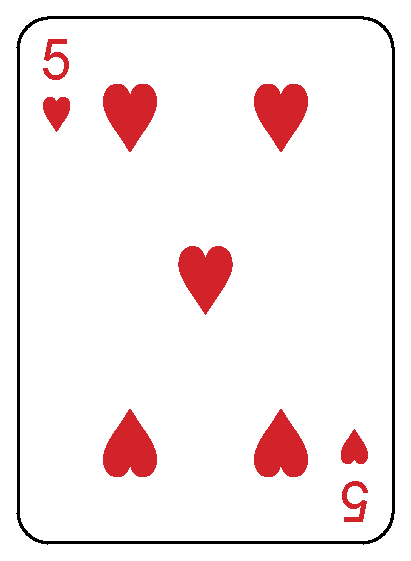
\includegraphics[width=0.15\linewidth]{images/cards/hearts_5}
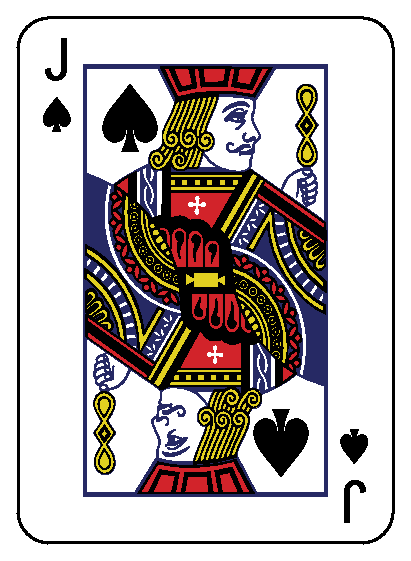
\includegraphics[width=0.15\linewidth]{images/cards/spades_jack}
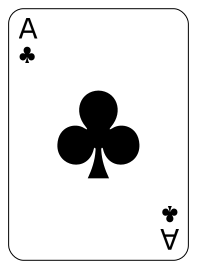
\includegraphics[width=0.15\linewidth]{images/cards/clubs_ace}
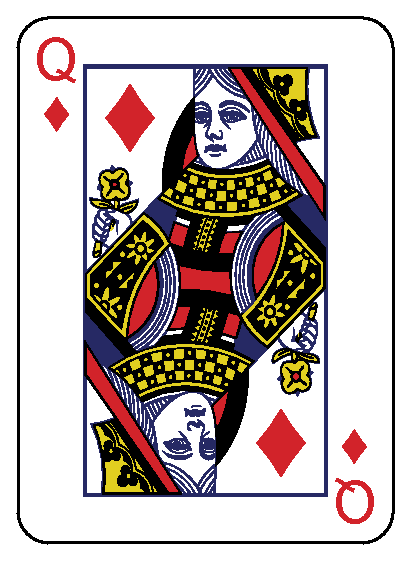
\includegraphics[width=0.15\linewidth]{images/cards/diamonds_queen}
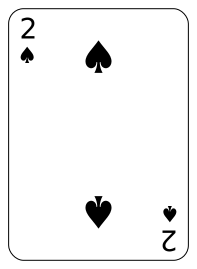
\includegraphics[width=0.15\linewidth]{images/cards/spades_2}

\begin{quote}
How many different 5 card poker hands are there?
\end{quote}

52 distinct cards, choose 5, order doesn't matter here, so the answer is \[\binom{52}{5} = \frac{52!}{47!\cdot 5!}=2,595,960.\]

Now let's consider a few types of poker hands.

A \textbf{Three of a Kind}\index{poker!Three of a Kind} is a hand of five cards that has 3 of one rank, and the other 2 cards do not have equal rank, such as this hand:

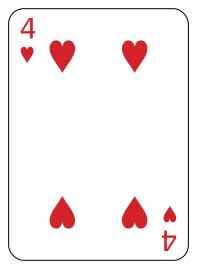
\includegraphics[width=0.15\linewidth]{images/cards/hearts_4}
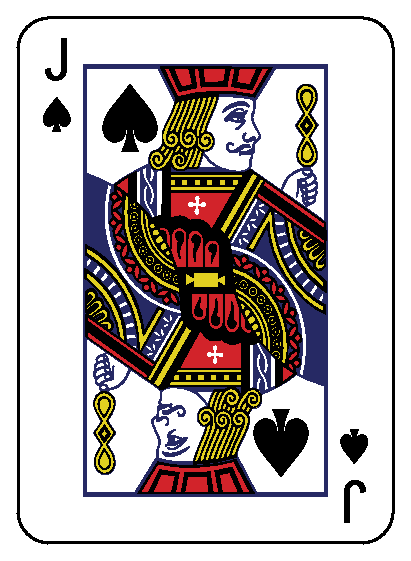
\includegraphics[width=0.15\linewidth]{images/cards/spades_jack}
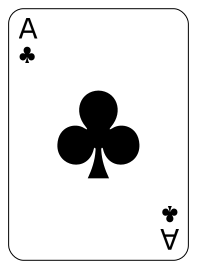
\includegraphics[width=0.15\linewidth]{images/cards/clubs_ace}
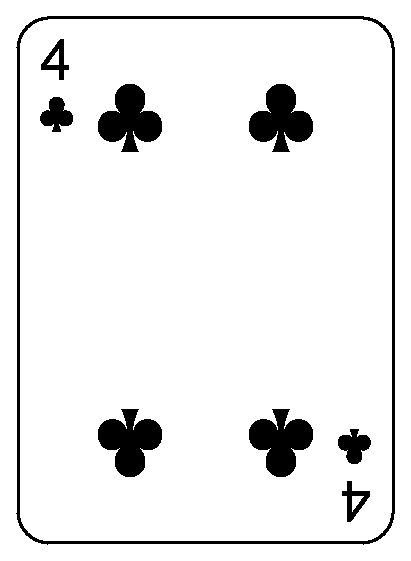
\includegraphics[width=0.15\linewidth]{images/cards/clubs_4}
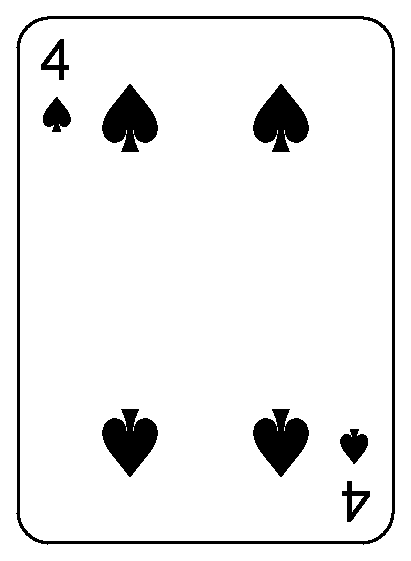
\includegraphics[width=0.15\linewidth]{images/cards/spades_4}

\begin{quote}
How many different ``Three of a Kind'' hands are there?
\end{quote}

We count the number of ways to build such a hand (we need to fill in each card with a rank and a suit).

\begin{enumerate}
\def\labelenumi{\arabic{enumi}.}
\tightlist
\item
  Pick the rank that appears 3 times - 13 choices.
\item
  Pick the 3 suits for this rank- we can choose 3 of the 4 possible suits in \(\binom{4}{3}\) ways.
\item
  Pick the remaining (distinct) 2 ranks - \(\binom{12}{2}\) ways (since the hand is unordered we do not impose an order on the choice of the remaining 2 ranks).
\item
  Pick the remaining 2 suits- each of the remaining 2 cards can have any of the 4 suits, we have \(4 \cdot 4\) ways to pick these suits.
\end{enumerate}

The total number of Three of a Kind hands is thus \[13\cdot\binom{4}{3}\cdot\binom{12}{2}\cdot4\cdot4 = 54912.\]

And we may reasonably define the probability of obtaining a 3-of-a-kind in a deal of 5 cards to be \[\frac{54912}{\binom{52}{5}}\approx 0.021.\]

\begin{quote}
How many different full house hands are possible?
\end{quote}

A \textbf{full house}\index{poker!full house} is a five card hand which has 3 cards of one rank, and 2 cards of another rank.

\begin{enumerate}
\def\labelenumi{\arabic{enumi}.}
\tightlist
\item
  Choose the rank that appears three times. We have \(\binom{13}{1} = 13\) ways to do this.
\item
  Choose three of the four suits for these three cards: \(\binom{4}{3}\).
\item
  Choose the rank that appears twice in the hand. We have 12 ranks left to choose from, so we have \(\binom{12}{1} = 12\) ways to do that.
\item
  Choose two of the four suits for the pair: \(\binom{4}{2}\).
\end{enumerate}

Completing these steps builds a full house, so we have
\[\binom{13}{1}\cdot\binom{4}{3}\cdot \binom{12}{1}\cdot \binom{4}{2} = 3744\] different full houses.

\begin{quote}
How many different ``Two Pair'' hands are possible?
\end{quote}

A \textbf{Two Pair}\index{poker!Two Pair} is a five card hand which has 3 cards of one rank, and 2 cards of another rank.

We present two arguments, but \emph{only one of them is correct}. Which is it?

First argument:

\begin{enumerate}
\def\labelenumi{\arabic{enumi}.}
\tightlist
\item
  Pick distinct ranks for the two pairs. We have \(\binom{13}{2}\) ways to do this.
\item
  Choose two of the four suits for one pair: \(\binom{4}{2}\).
\item
  Choose two of the four suits for the other pair: \(\binom{4}{2}\).
\item
  The fifth card can be any of the remaining 44 cards: \(\binom{44}{1}\).
\end{enumerate}

Second Argument:

\begin{enumerate}
\def\labelenumi{\arabic{enumi}.}
\tightlist
\item
  Pick the rank for the first pair. We have \(\binom{13}{1}\) ways to do this.
\item
  Choose two of the four suits for the first pair: \(\binom{4}{2}\).
\item
  Pick the rank for the second pair. We have \(\binom{12}{1}\) ways to do this.
\item
  Choose two of the four suits for the second pair: \(\binom{4}{2}\).
\item
  The fifth card can be any of the remaining 44 cards: \(\binom{44}{1}\).
\end{enumerate}

The first argument gives us this number:
\[\binom{13}{2}\cdot\binom{4}{2}\cdot \binom{4}{2} \cdot \binom{44}{1} = 123552.\]

The second argument gives us a number that is twice as big as the first:
\[\binom{13}{1}\cdot\binom{4}{2} \cdot \binom{12}{1} \cdot \binom{4}{2} \cdot \binom{44}{1} = 247104.\]
Which number is correct?

It turns out the second argument double counts. By picking the two ranks separately in the second argument, we impose an order on the ranks that is not a part of a poker hand. For instance, the second argument allows us to build the following famous Two Pair in two different ways:

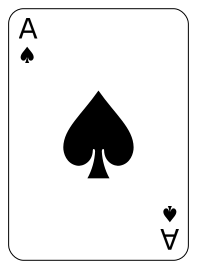
\includegraphics[width=0.15\linewidth]{images/cards/spades_ace}
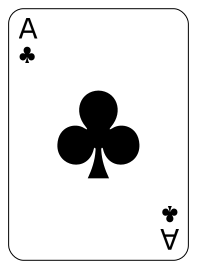
\includegraphics[width=0.15\linewidth]{images/cards/clubs_ace}
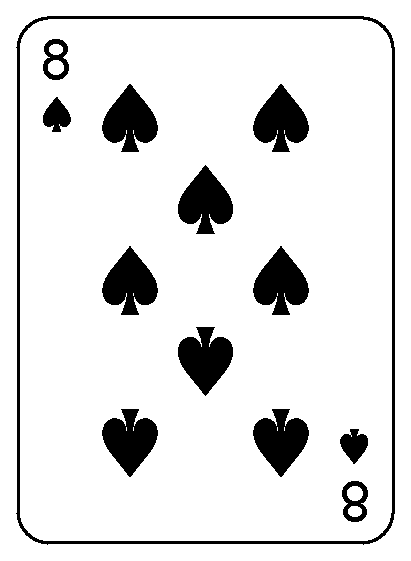
\includegraphics[width=0.15\linewidth]{images/cards/spades_8}
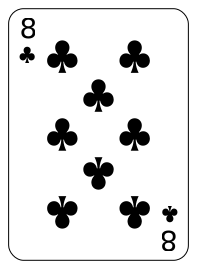
\includegraphics[width=0.15\linewidth]{images/cards/clubs_8}
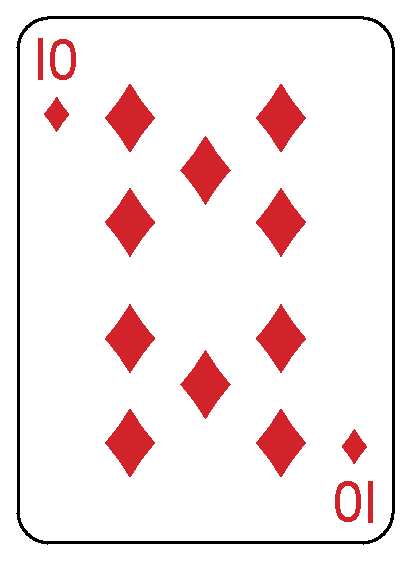
\includegraphics[width=0.15\linewidth]{images/cards/diamonds_10}

The first way to build the hand following the second argument:

\begin{enumerate}
\def\labelenumi{\arabic{enumi}.}
\tightlist
\item
  Choose the rank ace (A).
\item
  Choose the suits clubs and spades for the aces.
\item
  Choose the rank 8.
\item
  Choose the suits clubs and spades for the eights.
\item
  Choose the last card (10 of diamonds).
\end{enumerate}

The second way to build the hand following the second argument:

\begin{enumerate}
\def\labelenumi{\arabic{enumi}.}
\tightlist
\item
  Choose the rank 8.
\item
  Choose the suits clubs and spades for the eights.
\item
  Choose the rank A.
\item
  Choose the suits clubs and spades for the aces.
\item
  Choose the last card (10 of diamonds).
\end{enumerate}

In the end the two hands are the same because the order of the cards in your hand doesn't matter, so the second argument double counts. The first argument gives the correct answer.

The number of Two Pair hands is 123552.
\end{example}

\section{Multinomial Coefficients}\label{multinomial-coefficients}

Recall, \(\binom{n}{r}\) counts the number of ways to choose \(r\) from a set of \(n\). Effectively, then, \(\binom{n}{r}\) counts the number of ways to assign \(n\) elements to two groups of a specific size: \(r\) in the ``chosen'' group, and \(n-r\) in the ``not chosen'' group.

We can generalize this scene to \(k\) groups for \(k \geq 2\).

\begin{definition}
\protect\hypertarget{def:multinomial-coefficients}{}\label{def:multinomial-coefficients}Let
\[\binom{n}{n_1, n_2, \cdots, n_k}\] denote the number of ways of partitioning \(n\) distinct objects into \(k\) groups whose sizes are \(n_1, n_2, \ldots, n_k,\) where \(n_1 + n_2 + \cdots + n_k = n\). These expressions are called \textbf{multinomial coefficients}\index{multinomial coefficients}.
\end{definition}

Fact:
\begin{equation} 
  \binom{n}{n_1, n_2, \cdots, n_k} = \frac{n!}{n_1! \cdot n_2! \cdot \cdots \cdot n_k!}
  \label{eq:multinomial}
\end{equation}

Note that the binomial coefficent \(\displaystyle \binom{n}{r}\) can be written as a multinomial coefficent: \(\displaystyle \binom{n}{r, n-r}\).

\begin{example}
\protect\hypertarget{exm:Break-group-into-5}{}\label{exm:Break-group-into-5}A group of 15 volunteers will be split into 5 groups of 3, with each group working on a distinct project (weeding, spreading bark, setting up irrigation, constructing raised beds, and putting a roof on a shed).

\begin{quote}
How many distinct ways can the volunteers be split into five groups of three to work on these distinct projects?
\end{quote}

The multinomial coefficient
\[\binom{15}{3, 3, 3, 3, 3} = \frac{15!}{(3!)^5} = 168,168,000\]
counts the number of ways to do this if we treat the groups as distinct, which we should because the work done by each group is different: Mike in the weeding group is a much different scenario than Mike in the roof-raising group!
\end{example}

\begin{example}
\protect\hypertarget{exm:bananas}{}\label{exm:bananas}\leavevmode

\begin{quote}
How many ``words'' are spelled from the letters in `BANANAS.'
\end{quote}

If all seven letters in the word were distinct, we could form \(7!\) words, but we have repeat letters: 3 As, 2 Ns, 1 B, and 1 S.

We can arrive at the number of ``words'' from the `enumerate subtasks' approach:

We have to build a 7 letter word from the letters in BANANAS.

\begin{enumerate}
\def\labelenumi{\arabic{enumi}.}
\tightlist
\item
  Pick a location for the unique B: 7 choices
\item
  Pick a location for the unique S: 6 choices left
\item
  Choose 2 locations from the remaining 5 for the 2 identical Ns: \(\binom{5}{2}\)
\item
  Choose 3 locations from the remaining 3 for the 3 identical As: \(\binom{3}{3} = 1\)
\end{enumerate}

All told, we have \(7 \cdot 6 \cdot \binom{5}{2} \cdot \binom{3}{3} = 420\) ``words''.

Alternatively, the number of words equals the multinomial coefficient \[\binom{7}{3, 2, 1, 1} = 420\] because it counts the number of ways to assign 7 distinct elements (the 7 spots for letters in the word) into four groups of size 3, 2, 1, and 1 (3 locations for the As group, 2 for the Ns, 1 for the B and 1 for the S).

\end{example}

\section{Balls and Bins}\label{balls-and-bins}

Suppose I have 30 Watermelon \emph{Jolly Ranchers} to give away to 8 friends.

\begin{quote}
How many ways can I pass them out so that each person gets at least 1?
\end{quote}

To be precise, if we let \(n_i\) denote the number of jolly ranchers that person \(i\) receives (\(i\) runs from 1 to 8), I want to count how many different vectors \((n_1, n_2, \ldots, n_8)\) are possible with the conditions that each \(n_i \geq 1\) and the sum of the \(n_i\) equals 30.

To answer this question, we first consider balls and bins.

\begin{theorem}
\protect\hypertarget{thm:distribute-identical-balls-into-distinct-bins}{}\label{thm:distribute-identical-balls-into-distinct-bins}The number of ways to distribute \(n\) identical balls into \(r\) distinct bins is \[\binom{n+r-1}{r-1}.\]
\end{theorem}

\begin{proof}
Here's a proof strategy. Consider the following schematic of one way to distribute 8 balls into 3 bins:

\[\underline{\vert \text{ oo } \vert}~~~\underline{\vert \text{ oooo } \vert} ~~~ \underline{\vert \text{ oo } \vert}\]
We see two balls go into the first bin, 4 into the second, and 2 into the third. We can also represent this arrangement by pushing the bins together so that they share walls:

\[\underline{\vert \text{ oo } \vert \text{ oooo } \vert \text{ oo } \vert}\]

In fact, we don't really need those two outermost walls to communicate the arrangement, or the bin bottoms for that matter:

\[ \text{oo} \vert \text{oooo} \vert \text{oo}\]
So each distribution of the 8 balls into 3 bins corresponds to an ordered arrangement of 8 balls and 2 ``inner walls'', and we have \(\displaystyle\binom{10}{2}\) ways to choose the 2 spots for the inner walls from the 10 spots needed to create the arrangement.

More generally, with \(n\) balls and \(r\) bins we will have \(r-1\) inner walls, which leads us to the formula \[\binom{n+r-1}{r-1}.\]
\end{proof}

Let's return to the Watermelon \emph{Jolly Ranchers}.

In this scenario, the friends are the bins, and the candies are the balls, and the number of ways to distribute the candies to the 8 friends is \(\displaystyle \binom{30+8-1}{8-1}=\binom{37}{7},\)
which we can calculate in R: \texttt{choose(37,7)} = 10295472. I've got options.

However, this count doesn't answer the original question because it counts \emph{all} the ways to distribute the candies, including, say, all 30 going to one person. The original question here was to count the number of ways we can distribute the candies so that each friend gets at least 1.

So we do the following: first give each friend one \emph{Jolly Rancher}, then count the number of ways to distribute the remaining 22 using balls (22) and bins (8). It follows that the number of ways to distribute the candies so that each friend gets at least 1 is
\[\binom{22+8-1}{8-1} = \binom{29}{7},\]
which is \texttt{choose(29,7)} = 1560780. Still, I've got options.

\section{Calculating More Probabilities}\label{prob-with-counting-tools}

With our counting tools in hand, we can set about calculating the probability that an event \(A\) happens without having to first count every possible outcome in the sample space.

Here's the general scene in this section. We have some random experiment with finite sample space \(S,\) defined in such a way that the probability of each outcome in \(S\) is the same. In this case, the probability of any event \(A\) will simply be the size of the set \(A\) divided by the size of the set \(S\):
\[P(A) = \frac{|A|}{|S|}.\]

\begin{example}
\protect\hypertarget{exm:R-D-subcommittees}{}\label{exm:R-D-subcommittees}\leavevmode

\begin{quote}
Suppose we want to pick a 4 person subcommitee from a committee of 8 having 5 Republicans, and 3 Democrats. If we pick the subcommittee at random, what is the probability that all three Democrats are on it?
\end{quote}

The sample space \(S\) here is all possible subcommittees of size 4. Treating each of the 8 members as distinct people we have \[|S| = \binom{8}{4}.\]

The event \(A\) that all Democrats are in the subcommitte can be enumerated as follows:

\begin{enumerate}
\def\labelenumi{\arabic{enumi}.}
\tightlist
\item
  Choose all 3 Democrats for the subcommittee: \(\binom{3}{3} = 1\) way to do that!
\item
  Choose 1 Republican from 5 to fill out the subcommittee: \(\binom{5}{1} = 5.\)
\end{enumerate}

So \(|A|\) = 5, and using pencil and paper for this one:

\begin{align*}
P(A) &= \frac{5}{(8\cdot 7 \cdot 6 \cdot 5)/4!} \\
       &= \frac{4!}{8 \cdot 7 \cdot 6}\\
       &= \frac{4 \cdot 3 \cdot 2}{8 \cdot 7 \cdot 6}\\
       &= \frac{3}{7 \cdot 6}\\
       &= \frac{1}{7 \cdot 2}\\
       &=\frac{1}{14}.
\end{align*}

\end{example}

\begin{example}
\protect\hypertarget{exm:wine-expert}{}\label{exm:wine-expert}\leavevmode

\begin{quote}
A wine expert samples 8 wines blindly, two of which are genuinely ``high quality,'' and the others are ``budget wines.'' The expert chooses their 3 favorites. If they are really just picking at random, what is the probability that they pick both high quality wines?
\end{quote}

The sample space \(S\) consists of all possible ways to choose 3 from 8, and we consider each of these combinations of 3 equally likely.

We have \(\displaystyle |S| = \binom{8}{3} = 56.\)

The event of interest here, \(A,\) is choosing a combination that contains both ``high quality'' wines, and \(|A| = \displaystyle \binom{2}{2}\cdot\binom{6}{1} = 6\) (choose both of the high quality wines and choose one of the six budget wines). Thus,
\[P(A) = \frac{6}{56},\] about a 10\% chance of picking both high quality wines if, in fact, the expert is simply picking at random.

This probability is useful to know. If the expert does select both the high quality wines, does this suggest to you they know their business?

\end{example}

\begin{example}[Good Potatoes Bad Potatoes]
\protect\hypertarget{exm:potatoes}{}\label{exm:potatoes}A truck has 3000 potatoes (of which 75 are bad). We inspect 50 potatoes at random. We reject the shipment if more than two of the potates in the sample are bad.

\begin{quote}
What is the probability that we reject the shipment?
\end{quote}

We have 3000 potatoes, 2925 good potatoes, and 75 bad potatoes.

The sample space \(S\) here is all combinations of size 50, so \[|S| = \binom{3000}{50}.\]

The event of interest \(A\) is choosing a sample with more than 2 bad potatoes.

The number of samples of size 50 with 50 good and 0 bad potatoes is: \[\binom{2925}{50} \cdot \binom{75}{0}.\]
The number of samples of size 50 with 49 good and 1 bad potato is: \[\binom{2925}{49} \cdot \binom{75}{1}.\]
The number of samples of size 50 with 48 good and 2 bad potatoes is: \[\binom{2925}{48} \cdot \binom{75}{2}.\]

The number of samples with \emph{more than 2} bad potatoes is thus
\[|A| = |S| - \left[\binom{2925}{50} \cdot \binom{75}{0} +
\binom{2925}{49} \cdot \binom{75}{1} +
\binom{2925}{48} \cdot \binom{75}{2}\right],\]
and the probability of rejecting the sample is
\[P(A) = \frac{|A|}{|S|} \approx 0.1279.\]
\end{example}

\begin{example}[Poker II]
\protect\hypertarget{exm:poker-2}{}\label{exm:poker-2}\leavevmode

\begin{quote}
Determine the probabilty of drawing each of these standard 5 card poker hands: a Straight, a Flush, and a Straight Flush.
\end{quote}

Let's count some more types of poker hands. (We first looked at poker hands in Example \ref{exm:poker}.)

A \textbf{Straight Flush}\index{poker!Straight Flush} is a five cards poker hand in which all five suits are the same, and all five ranks form a run (either 2-6, 3-7, 4-8, 5-9, 6-10, 7-J, 8-Q, 9-K, 10-A).

A \textbf{Straight}\index{poker!Straight} consists of five cards such that all five ranks form a run and the hand is not a Straight Flush.

A \textbf{Flush}\index{poker!Flush} consists of five cards such that all five suits are the same and the hand is not a Straight Flush.

Here the sample space is \(S = \{\text{all possible 5 card hands}\},\) and we know \(|S| = \binom{52}{5}\).

How many different Straight Flushes are possible. Let's build one in steps, counting choices:

\begin{enumerate}
\def\labelenumi{\arabic{enumi}.}
\tightlist
\item
  Pick the low card for the run (which then determines all 5 ranks): 9 choices (2, 3, 4, 5, 6, 7, 8, 9, or 10)
\item
  Pick the one suit for all five cards: 4 choices.
\end{enumerate}

So there are \(9 \cdot 4 = 36\) Straight Flushes, and the probability of being dealt a Straight Flush is \[P(\text{Straight Flush}) = \frac{36}{\binom{52}{5}} \approx 0.00001385.\]

We now turn to the Straight.

As we saw in the case of the Straight Flush, we have 9 choices for the rank of the low card in a straight. Once that has been chosen, all five ranks are determined.

We have 4 choices for the suit of each of the 5 cards (allowing for the possibility that all five cards have the same suit), so \(9\cdot 4^5\) counts the number of Straights + Straight Flushes. The number of Straights is thus \(9 \cdot 4^5 - 36 = 9180\). It follows that \[P(\text{Straight}) = \frac{9180}{\binom{52}{5}} \approx 0.00353.\]

Finally, we count Flushes:

\begin{enumerate}
\def\labelenumi{\arabic{enumi}.}
\tightlist
\item
  Choose the flush suit: \(\binom{4}{1}\) ways.
\item
  Choose the 5 ranks: \(\binom{13}{5}\) ways.
\end{enumerate}

Then \(\displaystyle \binom{4}{1} \cdot \binom{13}{5} = 5148\) counts the number of Flushes, \emph{almost}. When we chose the 5 ranks, we allowed for the possibility that the ranks also formed a straight, so we must subtract out the Straight Flushes. The total number of Flushes: \(5148 - 36 = 5112.\)

So \[P(\text{Flush}) = \frac{5112}{\binom{52}{5}} = .00197.\]
So we have about a 1 in 500 chance of being dealt a Flush, and we note that a Flush is less common than a Straight (which is why a Flush beats a Straight in regular 5-card draw).

\end{example}

\begin{example}
\protect\hypertarget{exm:license-plates}{}\label{exm:license-plates}Classic Oregon license plates consist of 3 digits (0-9) followed by three letters (A-Z).

\begin{quote}
Find the probability that a randomly selected classic Oregon license plate has two 8s.
\end{quote}

The sample space \(S\) consists of all possible license plates, and \(|S| = 10^3\cdot 26^3,\) since order matters for license plates.

We enumerate the event \(A\) of drawing a plate with two 8s as follows:

\begin{enumerate}
\def\labelenumi{\arabic{enumi}.}
\tightlist
\item
  Choose the 2 spots for the 8s: \(\binom{3}{2} = 3\) choices
\item
  Pick the other number: \(9\) choices
\item
  Pick the three letters: \(26^3\) choices.
\end{enumerate}

So \[P(A) = \frac{3 \cdot 9 \cdot 26^3}{10^3\cdot 26^3} = \frac{27}{1000} = 0.027.\]
\end{example}

\begin{example}
\protect\hypertarget{exm:10sided-die}{}\label{exm:10sided-die}\leavevmode

\begin{quote}
Determine the probability that the first time we roll an 8 or higher with a 10-sided die is on the 5th roll.
\end{quote}

The sample space \(S\) consists of all sequences of 5 rolls of the die. For instance, \((4,5,2,9,5)\) is one element of \(S,\) and \(|S| = 10^5\).

The event of interest is \[A = \{ \text{roll 7 or lower in the first four rolls and 8 or higher on the 5th} \}.\]
Then \(|A| = 7^4 \cdot 3\) (7 choices for the 1st roll, 7 for the second, 7 for the 3rd, 7 for the 4th, and 3 for the 5th).

So \[P(A) = \frac{7^4 \cdot 3}{10^5}.\]

\end{example}

\begin{example}
\protect\hypertarget{exm:partition-set}{}\label{exm:partition-set}\leavevmode

\begin{quote}
A class has 12 people: 6 juniors, 4 sophomores, and 2 first-years. The class is randomly divided into 3 subgroups of size 5, 4, and 3. What is the probability that the 2 first-years are in the same subgroup?
\end{quote}

The sample space \(S\) consists of all possible partitions of the 12 people into the 3 subgroups, and we know

\begin{align*}
|S| &= \binom{12}{5,4,3} \\
    &= \frac{12!}{5! \cdot 4! \cdot 3!}\\ 
    &= \frac{12\cdot 11 \cdot 10 \cdot 9 \cdot 8 \cdot 7 \cdot 6}{24 \cdot 6}\\
    &= 27,720.
\end{align*}

The event of interest, \(A,\) consists of all partitions in which the two first-years are in the same subgroup. To count \(|A|\) we consider three cases:

Case 1: The two first-years are in the subgroup of 5. This means, after placing them in there, we have 10 people left to place in groups of size 3, 4, and 3, and we can do this in \[\binom{10}{3, 4, 3}\] ways.

Case 2: The two first-years are in the subgroup of 4, leaving 10 to place in groups of size 5, 2, and 3: \[\binom{10}{5,2,3}.\]

Case 3: The two first-years are in the subgroup of 3, which can happen in \[\binom{10}{5,4,1}\] ways.

So,\[|A| = \binom{10}{3, 4, 3} + \binom{10}{5, 2, 3} + \binom{10}{5, 4, 1},\] which evaluates to \(|A| = 7980\). So, \[P(A) = \frac{7980}{27720} \approx 0.288.\]

\end{example}

\chapter{Probability Theory}\label{probability-theory}

\section{Conditional Probability and Independence}\label{conditional-probability-and-independence}

Suppose we have a probability model associated to a sample space \(S\). If we are told some event \(B\) has occurred, how would the probability of other events change? Calculating a new probability for event \(A,\) given that \(B\) has occurred is called a conditional probability, and will be denoted \(P(A|B)\).

For instance, Let \(X\) denote the outcome if we roll a fair six-sided die. Let \(A\) be the event that we roll a 4, and \(B\) the event that we roll an even number. Since the die is fair, we expect that \(P(A) = 1/6\). Now suppose that the die is rolled and we are told that the event \(B\) has occurred. This leaves only three possible outcomes: 2, 4, and 6. The new, conditional probability of \(A\) given \(B\) would be \(P(A|B) = 1/3.\)

\begin{definition}
\protect\hypertarget{def:cond-prob}{}\label{def:cond-prob}The \textbf{conditional probability}\index{conditional probability} of an event \(A,\) given that an event \(B\) has occurred, denoted \(P(A|B),\) is
\begin{equation} 
  P(A|B) = \frac{P(A \cap B)}{P(B)},
  \label{eq:condprob}
\end{equation}
provided that \(P(B) > 0\).
\end{definition}

\begin{example}
For the 2023 Major League Baseball season, 328 hitters had at least 250 plate appearances. In this group, 71\% of them hit at least 10 HR for the season, and 31\% of them hit at least 20 HR. If you pick a player from this group at random, and you are told they hit over at least 10 HR, what is the probability that they hit at least 20 HR?

Let \(A\) be the event that the player hits at least 20 HR, and \(B\) the event that a player hit at least 10. Then we have been asked to find \(P(A|B)\). Note that \(A\) is a subset of \(B\) (if a player hit at least 20, then they also hit at least 10), so \(A \cap B\) = \(A,\) and it follows that
\begin{align*}
P(A|B) &= \frac{P(A \cap B)}{P(B)} \\
      &= \frac{P(A)}{P(B)} \\
      &= \frac{.31}{.71}\\
      &\approx .437.
\end{align*}
\end{example}

Note that from the conditional probability formula,

\[P(A \cap B) = P(B) \cdot P(A~|~B), \text{ provided }P(B)>0,\]
and that

\[P(A \cap B) = P(A) \cdot P(B~|~A), \text{ provided }P(A)>0.\]

\begin{definition}
Two events are called \textbf{independent}\index{independent events} if any of the following statements holds:

\begin{align*}
  P(A~|~B) &= P(A) \\
  P(B~|~A) &= P(B) \\
  P(A \cap B) &= P(A)\cdot P(B)
\end{align*}
\end{definition}

\begin{example}
The chance experiment ``roll a 6-sided die'' has sample space \(S = \{1, 2, 3, 4, 5, 6\}\).
Consider the events

\begin{align*}
A &= \{1,3,5\}\\
B &= \{1\}\\
C &= \{2\}\\
D &= \{1,2\}
\end{align*}

Then \(P(A) = 1/2, P(B) = 1/6, P(C) = 1/6,\) and \(P(D) = 1/3.\)

\textbf{Claim 1}: \(A\) and \(D\) are independent events.

\textbf{Reason 1}: Well, \(A \cap D = \{1\},\) so
\[P(A~|~D) = \frac{P(A\cap D)}{P(D)} = \frac{1/6}{1/3} = 1/2 = P(A).\]
\textbf{Claim 2}: \(B\) and \(C\) are not independent events.

\textbf{Reason 2}: \(B \cap C = \emptyset,\) so \[P(B~|~C) = \frac{P(B\cap C)}{P(C)} = \frac{0}{1/6} = 0 \neq P(B).\]

These simple examples help me remember that for events associated to a sample space,

\begin{quote}
independent is different than disjoint!
\end{quote}

In this example \(A\) and \(D\) are independent but not disjoint, while \(B\) and \(C\) are disjoint but not independent.
\end{example}

\begin{example}
\protect\hypertarget{exm:plumbing}{}\label{exm:plumbing}Suppose over the last five years, 10\% of all people in a town who have hired a plumber to do some work have been unhappy with the job that was done. One of the plumbers in the town is Frances. Frances has done 40\% of the plumbing jobs in town over these five years, and 25\% of all plumbing jobs that left the customer unhappy have been done by Frances.

\begin{quote}
Find the probability that a customer will be unhappy with the results if they hire Frances?
\end{quote}

We begin by translating what we know and what we want into symbols and probability notation.

Let \(S = \{ \text{all plumbing jobs in the town over the last 5 years} \}.\)

Let \(A = \{ \text{jobs handled by Frances} \}.\)

Let \(B = \{ \text{jobs in which the customer is unhappy} \}.\)

What do we want? \(P(B~|~A).\)

When do we want it? Now! So let's write down what we know.

What do we know?

\begin{itemize}
\tightlist
\item
  10\% of the jobs have left the customer unhappy \(~~\Rightarrow~~~~ P(B) = 0.1\).
\item
  Frances has done 40\% of all jobs \(~~\Rightarrow~~~~ P(A) = 0.4\).
\item
  25\% of all complaints dealt with Frances \(~~\Rightarrow~~~~ P(A~|~B) = 0.25\).
\end{itemize}

Well,
\begin{align*}
P(B~|~A) &= \frac{P(A\cap B)}{P(A)} \\
         &= \frac{P(A ~|~B)\cdot P(B)}{P(A)} \\
         &= \frac{(0.25)(0.1)}{(0.4)} \\
         &= 0.0625.
\end{align*}

Ok, there is about a 6 percent chance that a customer will be unhappy with their plumbing job if they hire Frances.

An irresponsible person who wants to be intentionally misleading could rant in all caps ``25 PERCENT OF UNHAPPY CUSTOMERS HIRED FRANCES!!!'' Let's be better than that. Knowing the full context here, which includes what proportion of the town's plumbing jobs have gone to Frances, is necessary to establish how effective Frances has been as a plumber these last five years.
\end{example}

\begin{example}
\leavevmode

\begin{quote}
Roll 2 6-sided dice. What is the probability that both values are less than 3?
\end{quote}

We assume the two dice are independent. (What appears on one die is independent of what appears on the other.)

Let \(A = \{ \text{first die is less than 3}\}\) and \(B = \{ \text{second die is less than 3}\}.\)

``Less than 3'' means ``1 or 2'' so \(P(A) = P(B) = 2/6 = 1/3.\)
The question asks for \(P(A \cap B).\) Since \(A\) and \(B\) are independent, \[P(A \cap B) = P(A)\cdot P(B) = (1/3)\cdot(1/3) = 1/9.\]

We remark that we can also use counting techniques to find this probability directly, as in Section \ref{prob-with-counting-tools}, as follows.

The sample space \(S\) of this chance experiment consists of all possible rolls of the two dice. That is, \(S\) consists of all ordered pairs of the form \((i,j)\) with \(i, j \in \mathbb{N}\) and \(1\leq i, j \leq 6,\) and \(|S| = 6^2\). The event of interest, \(E,\) consists of all rolls \((i,j)\) in \(S\) such that \(i, j \leq 2\). So, \(|E| = 2^2,\) and \(P(E) = 4/36 = 1/9\).

So, thinking of the chance experiment as a sequence of independent events we calculate the probability of interest as \(\frac{2}{6} \cdot \frac{2}{6},\) and thinking of the probability via the ``(outcomes of interest)/(all possible outcomes)'' approach we think of the probability as \(\frac{2\cdot 2}{6 \cdot 6}\).

\end{example}

\begin{example}
\protect\hypertarget{exm:four-on-rolll-8}{}\label{exm:four-on-rolll-8}Roll a regular 6-sided die until a 4 comes up. What is the probability that this occurs on the 8th roll?

The values of the rolls are independent events, the probability of not rolling a four on a given roll is 5/6, and the probability of rolling a 4 is 1/6. It follows that the probability of rolling 7 non-4s followed by one 4 is
\[P(\text{first 4 on roll 8}) = \left(\frac{5}{6}\right)^7 \cdot \left(\frac{1}{6}\right).\]
More generally, the probability that our first 4 comes up on roll \(n\) (for any \(n \in \mathbb{N}\)) will be
\[P(\text{first 4 on roll }n) = \left(\frac{5}{6}\right)^{n-1} \cdot \left(\frac{1}{6}\right).\]
\end{example}

\section{Two Laws of Probability}\label{two-laws-of-probability}

\begin{theorem}
\protect\hypertarget{thm:two-prob-laws}{}\label{thm:two-prob-laws}

Suppose \(A\) and \(B\) are two events.

\begin{enumerate}
\def\labelenumi{\arabic{enumi}.}
\item
  \textbf{Multiplicative Law of Probability}:\index{probability!multiplicative law}
  \begin{align*}
    P(A \cap B) &= P(A)\cdot P(B~|~A) \\
             &= P(B) \cdot (A~|~B) 
    \end{align*}
\item
  \textbf{Additive Law of Probability}:\index{probability!additive law}
  \[P(A\cup B) = P(A) + P(B) - P(A \cap B).\]
\end{enumerate}

\end{theorem}

\begin{proof}
\leavevmode

\begin{enumerate}
\def\labelenumi{\arabic{enumi}.}
\item
  This proof follows directly from the definition of conditional probability (\ref{def:cond-prob}).
\item
  For finite sets \(A\) and \(B,\) we know \[|A \cup B| = |A| + |B| - |A \cap B|,\] from which the result follows.
\end{enumerate}

More generally, for any sets \(A\) and \(B,\) the union \(A \cup B\) can be decomposed into disjoint sets: \(A \cup B = A \cup (\overline{A} \cap B).\)
So, \[P(A \cup B) = P(A) + P(\overline{A} \cap B).\]

Similarly, we can decompose the set \(B\) into disjoint sets as follows: \(B = (\overline{A} \cap B) \cup (A \cap B).\)
So \[P(B) = P(\overline{A}\cap B) + P(A \cap B).\]
Combining these two probability equations we see \[P(A \cup B) = P(A) + \left[P(B)-P(A\cap B)\right],\] which completes the proof.

\end{proof}

Next, consider three events, \(A_1, A_2, A_3\). Notice that

\begin{align*}
P(A_1 \cap A_2 \cap A_3) &= P((A_1\cap A_2) \cap A_3) \\
                         &= P(A_1 \cap A_2) \cdot P(A_3~|~A_1 \cap A_2)\\
                         &= P(A_1) \cdot P(A_2~|~A_1) \cdot P(A_3~|~A_1 \cap A_2).
\end{align*}

This formula may be extended to the intersection of any number of sets.

\begin{equation} 
  P(A_1 \cap \cdots \cap A_k) = P(A_1) \cdot P(A_2 ~|~ A_1) \cap  \cdots \cap P(A_k ~|~ (A_1 \cap \cdots \cap A_{k-1}))
  \label{eq:prob-intersection}
\end{equation}

\begin{example}
\protect\hypertarget{exm:all-hearts}{}\label{exm:all-hearts}Flip over 4 cards from a regular 52-card deck. What is the probability they are all hearts?

We flip the cards over one at a time, and define the four events \(A_i\) = the event that card \(i\) is a hearts, for \(i = 1, 2, 3, 4\).

We want the probability that all four events occur. That is, we want \(P(A_1 \cap A_2 \cap A_3 \cap A_4),\) and we find this using Equation \eqref{eq:prob-intersection}.

\begin{align*}
P(A_1 \cap A_2 \cap A_3 \cap A_4) &= P(A_1) \cdot P(A_2 ~|~ A_1) \cdot P(A_3 ~|~ A_1 \cap A_2) \cdot P(A_4 ~|~ A_1 \cap A_2 \cap A_{3})\\
&= \frac{13}{52} \cdot \frac{12}{51} \cdot \frac{11}{50} \cdot \frac{10}{49} \\
&\approx 0.0026.
\end{align*}
\end{example}

\begin{example}
\protect\hypertarget{exm:mult-law}{}\label{exm:mult-law}\leavevmode

\begin{quote}
Find the probability that a random 4 digit number has distinct odd digits.
\end{quote}

Two notes: We have 5 odd digits, and the leading (thousands) digit of a 4-digit number cannot be 0.

Using the multiplicative law of probability we calculate the probability of a sequence of events and multiply them:

\begin{itemize}
\tightlist
\item
  The probability that the leading digit is odd: 5/9.
\item
  The probability that the 2nd digit is odd, given the first was: 4/10.
\item
  The probability that the 3rd digit is odd, given the first two were: 3/10.
\item
  The probability that the 4th digit is odd, given the first three were: 2/10.
\end{itemize}

By the multiplicative law of probability, the probability that a random 4-digit number has distinct odd digits is \[\frac{5}{9} \cdot \frac{4}{10} \cdot \frac{3}{10} \cdot \frac{2}{10} \approx 0.0133.\]

\end{example}

We have three corollaries to Theorem \ref{thm:two-prob-laws}.

\begin{corollary}
\protect\hypertarget{cor:comp-prob}{}\label{cor:comp-prob}For any event \(A,\) \[P(\overline{A}) = 1 - P(A).\]
\end{corollary}

\begin{proof}
By the additive law, \[P(A \cup \overline{A}) = P(A) + P(\overline{A})-P(A \cap \overline{A}).\]
Since \(A\cup \overline{A} = S\) and \(A \cap \overline{A} = \emptyset,\) \(P(A \cup \overline{A}) = 1\) and \(P(A \cap \overline{A}) = 0,\) so \[1 = P(A) + P(\overline{A}),\] and the result follows.
\end{proof}

\begin{corollary}
If \(A\) and \(B\) are disjoint events, then \(P(A \cup B) = P(A) + P(B).\)
\end{corollary}

\begin{proof}
Since \(A\cap B = \emptyset,\) \(P(A \cap B) = 0\) and the result follows from the Additive Law of Probability.
\end{proof}

\begin{corollary}
For three events \(A, B, C\).

The probability of their union is

\begin{align*}
P(A \cup B \cup C) &= P(A)+P(B)+P(C)\\
                   &~~~~ - [P(A\cap B) + P(A \cap C) + P(B \cap C)]\\
                   &~~~~ + P(A \cap B \cap C).
\end{align*}

The probability of their intersection is
\[P(A \cap B \cap C) = P(A) \cdot P(B~|~A) \cdot P(C ~|~ A \cap B).\]
\end{corollary}

\begin{proof}
First we tackle the union case by appealing to the additive law of probability twice, along a the distributive law of sets.

\begin{align*}
P(A \cup B \cup C) &= P(A \cup (B \cup C)) \\
                   &= P(A) + P(B \cup C) - P(A \cap (B \cup C)) \\
                   &= P(A) + [P(B) + P(C)- P(B \cap C)] - P((A\cap B) \cup (A \cap C)) \\
                   &= P(A) + P(B) + P(C) - P(B \cap C) \\
                   &~~~~ - [P(A \cap B)+ P(A \cap C)-P((A \cap B) \cap (A \cap C))]\\
                   &= P(A) + P(B) + P(C) \\
                   &~~~~ - [P(A\cap B) + P(A \cap C) + P(B \cap C)] \\
                   &~~~~ + P((A \cap B) \cap (A \cap C))
\end{align*}

from which the result follows since \(A \cap B \cap A \cap C = A \cap B \cap C\).

For the intersection case, by definition of conditional probability the right hand side of the equation is
\[\text{RHS } = P(A) \cdot \frac{P(A \cap B)}{P(A)} \cdot \frac{P(C\cap A\cap B)}{P(A \cap B)},\] and the result follows by cancellation.
\end{proof}

\section{Event-Composition Method}\label{event-composition-method}

In some examples in this chapter we've been using a method for calculating probabilities called the event-composition method, which can be described as follows.

\begin{quote}
\textbf{Event-Composition Method}:\index{event-composition method} Describe the sample space and relevant events; write down what information we're given regarding probabilities etc. via the symbols representing these events; Express what we want to know via these symbols, and use our probability laws to use what we know to determine what we want.
\end{quote}

\begin{example}
\protect\hypertarget{exm:craps-4-before-7}{}\label{exm:craps-4-before-7}Two regular 6-sided dice are rolled until we roll a sum of 4 or a sum of 7.

\begin{quote}
What is the probability that we roll a 4 before we roll a 7?
\end{quote}

We define two key events:

\begin{itemize}
\tightlist
\item
  \(A\): we roll a sum of 4; and
\item
  \(B\): we do not roll a 4 or 7.
\end{itemize}

From our handy \(6 \times 6\) grid describing all possible sums when rolling 2 dice (Example \ref{exm:roll2dice}), we know \[P(A) = \frac{3}{36}, ~~P(B) = \frac{27}{36}.\]

In this game we roll the dice until we roll a 4 or a 7, and we \textbf{win} if we roll a 4 before rolling a 7.

There is no limit to how many rolls we might need in order to win.
We might win on the 1st roll, or the 2nd roll, or the 3rd roll, or the 4th roll, \ldots{} etc. In fact, for each \(n \in \mathbb{N},\) we might win on roll \(n\).

Put another way, we can partition the event of winning into a countably infinite collection of mutually disjoint events: winning on roll 1, winning on roll 2, winning on roll 3, etc. Then,
\[P(\text{winning}) = \sum_{n=1}^\infty P(\text{winning on roll }n).\]

The probability of winning on the 1st roll is \(P(A)\).

The probability of winning on the 2nd roll is \(P(B) \cdot P(A)\) (no 4 or 7 on 1st roll and yes 4 on the 2nd roll).

The probability of winning on the 3rd roll is \(P(B) \cdot P(B) \cdot P(A),\) and, more generally, the probability of winning on roll \(n\) is \[P(B)^{n-1}\cdot P(A).\]

The sum of these probabilities is an honest-to-goodness-living-in-the-wild geometric series:

\begin{align*}
P(\text{4 before 7}) &= \sum_{n=1}^\infty P(B)^{n-1}P(A)\\
                     &= P(A)\sum_{n=0}^\infty P(B)^n\\
                     &= \frac{3}{36}\sum_{n=0}^\infty \left(\frac{27}{36}\right)^n
\end{align*}

As a reminder, the sum of a geometric series is given by
\begin{equation}
\sum_{n=0}^\infty r^n = \frac{1}{1-r} \text{ if } |r| < 1
\label{eq:geometric-series}
\end{equation}

Using this formula with \(r = 27/36,\) we see the probability that we roll a 4 before a 7 is \[P(\text{4 before 7}) = \frac{3}{36}\cdot \frac{1}{1-(27/36)} = \frac{1}{3}.\]
\end{example}

\section{Bayes' Rule}\label{bayes-rule}

\begin{definition}
\protect\hypertarget{def:partition}{}\label{def:partition}

A collection \(\{B_1, B_2, \ldots, B_n\}\) of nonempty subsets of \(S\) is called a \textbf{partition}\index{partition} of \(S\) provided that

\begin{enumerate}
\def\labelenumi{\arabic{enumi}.}
\tightlist
\item
  \(S = B_1 \cup B_2 \cup \cdots \cup B_n,\) and
\item
  the collection is pairwise disjoint.
\end{enumerate}

\end{definition}

\begin{theorem}[Law of Total Probability]
\protect\hypertarget{thm:total-law-prob}{}\label{thm:total-law-prob}Assume \(\{B_1, B_2, \ldots, B_k\}\) is a partition of the sample space \(S,\) and \(P(B_i) > 0\) for each \(i = 1, 2, \ldots k\). Then for any event \(A,\) \[P(A) = \sum_{i=1}^k P(A~|~B_i)\cdot P(B_i).\]
\end{theorem}

\begin{proof}
Notice that as a set,
\begin{align*}
A &= A \cap S \\
  &= A \cap (B_1 \cup B_2 \cup \cdots \cup B_k) \\
  &= (A \cap B_1) \cup (A \cap B_2) \cup \cdots \cup (A \cap B_k).
\end{align*}

Furthermore, since the \(B_i\) are pairwise disjoint, the \((A \cap B_i)\) are pairwise dijoint as well, and by the additive law of probability \[P(A) = \sum_{i = 1}^k P(A \cap B_i).\]

The result then follows since each \(P(A \cap B_i) = P(A~|~B_i)\cdot P(B_i)\).
\end{proof}

\begin{example}
\protect\hypertarget{exm:ad-agency}{}\label{exm:ad-agency}An ad agency notices

\begin{itemize}
\tightlist
\item
  1 in 50 potential buyers of a particular product sees an advertisement for it on television
\item
  1 in 5 potential buyers sees the ad on YouTube.
\item
  1 in 100 sees the ad on both TV and YouTube.
\item
  1 in 3 potential buyers actually purchase the product after seeing an ad, and
\item
  1 in 10 potential buyers buy it without seeing an ad.
\end{itemize}

\begin{quote}
What is the probability that a radnomly selected potential buyer will purchase the product?
\end{quote}

We define relevant events for the sample space \(S = \{ \text{ all potential buyers }\}\). In particular, we let

\begin{itemize}
\tightlist
\item
  \(A\) = the set of potential buyers who purchase the product,
\item
  \(B\) = the set of potential buyers who see the ad on TV,
\item
  \(C\) = the set of potential buyers who see the ad on YouTube.
\end{itemize}

Next we translate what we know and what we want into symbols.

What we want: \(P(A)\).

What we know:

\begin{itemize}
\tightlist
\item
  \(P(B) = 1/50,\)
\item
  \(P(C) = 1/5,\)
\item
  \(P(B \cap C) = 1/100,\)
\item
  \(P(A ~|~ B \cup C) = 1/3,\) and
\item
  \(P(A ~|~ \overline{B \cup C}) = 1/10.\)
\end{itemize}

We also know by the additive law of probability that

\[P(B \cup C) = \frac{1}{50} + \frac{1}{5} - \frac{1}{100} = \frac{21}{100},\] so by Corollary \ref{cor:comp-prob}, \[P(\overline{B \cup C}) = 1 - \frac{21}{100} = \frac{79}{100}.\]
Finally, notice that since \(B \cup C\) and \(\overline{B \cup C}\) partition the sample space, \[A = \left[A \cap (B \cup C)\right] \cup \left[A \cap (\overline{B \cup C})\right],\] where these two sets are disjoint.

By the Law of Total Probability,

\begin{align*}
P(A) &= P(A \cap (B \cup C)) + P(A \cap (\overline{B \cup C)})\\
     &= P(B \cup C) \cdot P(A ~|~ B \cup C) + P(\overline{B \cup C})\cdot P(A~|~\overline{B \cup C})\\
     &= \frac{21}{100} \cdot {1}{3} + \frac{79}{100}\cdot {1}{10} \\
     &= \frac{7}{100} \cdot \frac{7.9}{100} \\
     &= 0.149.
\end{align*}
\end{example}

\begin{example}
\protect\hypertarget{exm:bayes-intro}{}\label{exm:bayes-intro}Suppose you have taken a test for a deadly disease. The doctor tells you that the test is quite accurate in that if you have the disease then the test will correctly tell you that you have the disease 100\% of the time. However, if you don't have the disease, the test will very occasionally (1 time in 10) mistakenly tell you that you have it.

The test comes back positive (it says you have the disease)! Are you worried!? In particular, can you estimate the probability that you actually have the disease given that the test came back positive?

What information were we given? What information do we want?

We were given:

\begin{itemize}
\tightlist
\item
  The probability of a positive test given I have the disease is 1.
\item
  The probability of a positive test given I do not have the disease is 0.1
\end{itemize}

We want:

\begin{itemize}
\tightlist
\item
  The probability I have the disease given that I have a positive test.
\end{itemize}

Let \(A\) denote the event that I have a positive test, \(B\) the event that I have the disease.

Then I want \(P(B|A)\) and I know \(P(A|B) = 1\) and \(P(A|\overline{B}) = 0.1.\)

It turns out I need more information than I've been given to answer this question, as the following scenarios demonstrate.

\emph{Scenario 1}: Suppose the population consists of 100 people, and 50 people, in fact, have the disease (blue - healthy, red - sick in the figure below). Then, if we tested each individual we would find 55 positive tests (the circled dots below) (all 50 of the sick people would test positive, and 10\% of the 50 healthy people, so 5 healthy people would also test positive.)

\begin{figure}
\centering
\pandocbounded{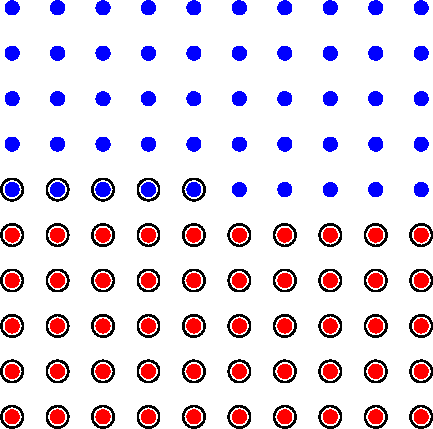
\includegraphics[keepaspectratio]{math340-notes_files/figure-latex/50-50-sick-1.pdf}}
\caption{\label{fig:50-50-sick}50\% of population has the disease}
\end{figure}

In this scenario, given that I tested positive, there is a 50/55 chance that I have the disease.

\emph{Scenario 2}: Suppose the population consists of 100 people, and 1 person, in fact, has the disease (blue - healthy, red - sick in the figure below). Then, if we tested each individual we would find about 11 positive tests (the circled dots below) (the one sick people would test positive, and 10\% of the 99 healthy people, so about 10 healthy people would also test positive.)

\begin{figure}
\centering
\pandocbounded{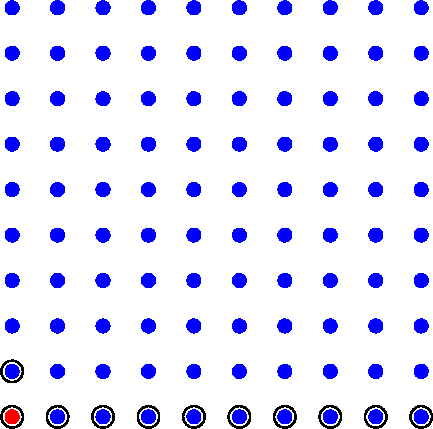
\includegraphics[keepaspectratio]{math340-notes_files/figure-latex/1-99-sick-1.pdf}}
\caption{\label{fig:1-99-sick}1\% of population has the disease}
\end{figure}

In this scenario, given that I tested positive, there is a 1/11 chance that I have the disease.

So, it seems to answer the question in this example, it is important to know what percentage of the population have the disease. Baye's Theorem below tells us that this is all the additional information we need.
\end{example}

\begin{theorem}[Bayes' Rule]
\protect\hypertarget{thm:Bayes-rule}{}\label{thm:Bayes-rule}Assume \(\{B_1, B_2, \ldots, B_k\}\) is a partition of the sample space \(S,\) and \(P(B_i) > 0\) for each \(i = 1, 2, \ldots k\). Then for any particular \(B_j,\) \[P(B_j ~|~ A) = \frac{P(A~|~B_j)\cdot P(B_j)}{\sum_{i=1}^k P(A~|~B_i)\cdot P(B_i)}.\]
\end{theorem}

\begin{example}
\protect\hypertarget{exm:bad-apples}{}\label{exm:bad-apples}A grocery store has an apple bin. 70\% of the apples are Liberty, and 30\% are Braeburn. From past experience, we know that 8\% of Liberty apples are bad, and 15\% of Braeburn apples are bad. Suppose you pick an apple at random and find it is bad. What is the probability that the apple is a Braeburn?

We define our relevant sets.

\begin{itemize}
\tightlist
\item
  \(S\) = all apples in the bin
\item
  \(B_1\) = all Liberty apples in \(S\)
\item
  \(B_2\) = all Braeburn apples in \(S\) (and the \(B_i\) partition \(S\)!)
\item
  \(A\) = bad apples in \(S\).
\end{itemize}

We know:

\begin{itemize}
\tightlist
\item
  \(P(B_1) = .7,\) and \(P(B_2) = .3\)
\item
  \(P(A~|~B_1) = .08,\) and \(P(A~|~B_2) = .15\).
\end{itemize}

We want:

\begin{itemize}
\tightlist
\item
  \(P(B_2 ~|~ A)\).
\end{itemize}

This task calls for Bayes' Rule.

\[P(B_2~|~A) = \frac{P(A~|~B_2)\cdot P(B_2)}{P(A~|~B_1)\cdot P(B_1)+P(A~|~B_2)\cdot P(B_2)}.\]
We know each probability in the right-hand side of the equation:
\[P(B_2~|~A) = \frac{(.15)(.3)}{(.08)(.7)+(.15)(.3)} \approx .446.\]
About a 44\% chance that if we drew a bad apple it's a Braeburn.

We can also use a tree diagram to arrive at this answer:

\begin{figure}
\centering
\pandocbounded{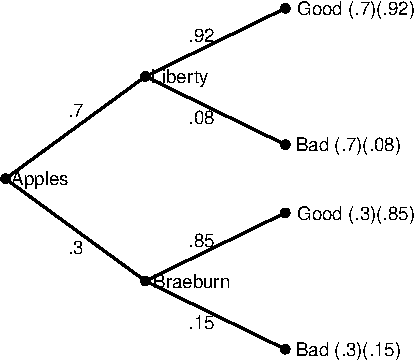
\includegraphics[keepaspectratio]{math340-notes_files/figure-latex/bayes-apple-1.pdf}}
\caption{\label{fig:bayes-apple}Picking an Apple}
\end{figure}

From the diagram, the probability of picking a bad apple is \((.7)(.08) + (.3)(.15)\) and the probability of picking a bad Braeburn is \((.3)(.15),\) so the probability of having picked a Braeburn, given we picked a bad apple is \[\frac{(.3)(.15)}{(.7)(.08) + (.3)(.15)}.\]
\end{example}

\begin{example}
\protect\hypertarget{exm:factory-skill}{}\label{exm:factory-skill}

Two methods, \(A\) and \(B\) are available for teaching a certain skill at a factory. The failure rate for \(A\) is 20\%, and for \(B\) is 10\%. However, \(B\) is more expensive and is used only 30\% of the time (\(A\) is used the other 70\%). A worker was taught the skill by one of the methods but failed to learn it correctly. What is the probability they were taught by Method \(A\)?

Let \(S\) denote the sample space of all workers who have been trained in this skill.

We have this partition of \(S\):

\begin{itemize}
\tightlist
\item
  \(A\) = those taught by method \(A\)
\item
  \(B\) = those taught by method \(B\).
\end{itemize}

We also have \(F\) = those who fail to learn the skill correctly.

We want: \(P(A~|~F)\).

We know: \(P(A) = .7,\) \(P(B) = .3,\) \(P(F~|~A) = .2,\) and \(P(F~|~B) = .1\).

Using Bayes' Rule,
\begin{align*}
P(A~|~F) &= \frac{P(A)\cdot P(F~|~A)}{P(A)\cdot P(F~|~A)+P(B)\cdot P(F~|~B)}\\
&= \frac{(.7)(.2)}{(.7)(.2)+(.3)(.1)}\\
&\approx .82.
\end{align*}
Given a worker failed to learn the skill, there is about an 82\% chance they had been taught by Method \(A\).

\begin{figure}
\centering
\pandocbounded{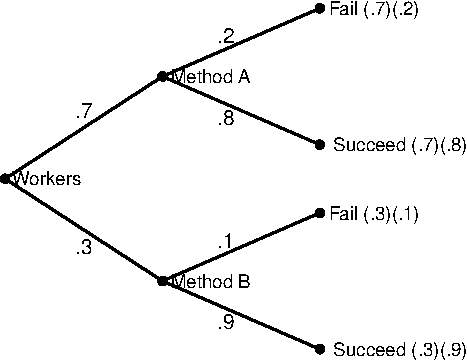
\includegraphics[keepaspectratio]{math340-notes_files/figure-latex/bayes-instruct-method-1.pdf}}
\caption{\label{fig:bayes-instruct-method}Learning by a Method}
\end{figure}

\end{example}

\chapter{Discrete Random Variables}\label{discrete-random-variables}

Recall, a random variable \(X\) is a real-valued function defined over a sample space associated with a chance experiment.

The \textbf{space of \(X\)}\index{random variable!space} is the set of possible outcomes for \(X,\) and a \textbf{probability model} for \(X\) is an assignment \(p(x)\) to each \(x\) in the space of \(X\) such that

\begin{itemize}
\tightlist
\item
  each \(p(x) \geq 0,\) and
\item
  the sum of all the \(p(x)\) equals 1.
\end{itemize}

Let's look at some examples.

\begin{example}
\protect\hypertarget{exm:draw-2-balls}{}\label{exm:draw-2-balls}Five balls numbered 1 through 5 are placed in a hat. Two balls are randomly selected without replacement. We consider two random variables associated to this chance experiment:

\begin{itemize}
\tightlist
\item
  \(X\) is the largest of the two selected balls, and
\item
  \(Y\) is the sum of the two selected balls.
\end{itemize}

\begin{quote}
Find the space of \(X,\) the space of \(Y,\) and reasonable probability models for both random variables.
\end{quote}

OK, drawing two balls from five, without replacement, we have \(\binom{5}{2} = 10\) possible outcomes. These 10 possible outcomes form the sample space associated with the chance experiment, and we assume each of these 10 outcomes is equally likely.

We can brute-force our answers by following the sample-point method: list all the sample points, and go!

\begin{table}[!h]
\centering
\caption{\label{tab:balls-from-hat-rv}Two random variables associated with drawing two balls from a hat.}
\centering
\begin{tabular}[t]{>{}l||c|c|c|c|c|c|c|c|c|c}
\hline
S & \{1,2\} & \{1,3\} & \{1,4\} & \{1,5\} & \{2,3\} & \{2,4\} & \{2,5\} & \{3,4\} & \{3,5\} & \{4,5\}\\
\hline
X & 2 & 3 & 4 & 5 & 3 & 4 & 5 & 4 & 5 & 5\\
\hline
Y & 3 & 4 & 5 & 6 & 5 & 6 & 7 & 7 & 8 & 9\\
\hline
\end{tabular}
\end{table}

Again, we assume each of the 10 elements in \(S\) is equally likely, so the probability that \(X = 4,\) say, will be the 3/10 since \(X\) takes the value 4 for 3 of the 10 elements in \(S\).

The probability model for \(X\) in table form:
\[
\begin{array}{c|c|c|c|c}
x    &  2 &  3 &  4 &  5 \\ \hline
p(x) & .1 & .2 & .3 & .4 
\end{array}
\]

The probability model for \(Y\) in table form:
\[
\begin{array}{c|c|c|c|c|c|c|c}
y & 3 & 4 & 5 & 6 & 7 & 8 & 9\\ \hline
p(y) & .1 & .1 & .2 & .2 & .2 &.1 & .1 
\end{array}
\]
Observe that in each case, we have a valid probability model. Each probability is non-negative, and \(\sum_x p(x) = 1\) and \(\sum_y p(y) = 1\).
\end{example}

\begin{example}
\protect\hypertarget{exm:roll-until-4}{}\label{exm:roll-until-4}Let \(X\) equal the number of rolls of a 6-sided die needed to roll your first 4.

\begin{quote}
Find the space of \(X\) and give a reasonable probability model for \(X\).
\end{quote}

The space of \(X\) is \(\mathbb{N} = \{1, 2, 3, \ldots \}\).

We assume each of the 6 values is equally likely on any given roll, and that the values are independent from roll to roll. So, the probability of rolling a 4 is 1/6, and the probability of not rolling a 4 is 5/6. Then, the probability of rolling our first 4 on roll \(x,\) for each \(x \geq 1,\) is
\[P(X = x) = \left(\frac{5}{6}\right)^{x-1}\cdot\frac{1}{6}.\]

Is this a valid probability model? Certainly each probability is non-negative. Do they all sum to 1? This requires the geometric series formula from Calc II to check:

\begin{align*}
\sum_{x = 1}^\infty \left(\frac{5}{6}\right)^{x-1}\frac{1}{6} &= \frac{1}{6}\sum_{x = 0}^\infty \left(\frac{5}{6}\right)^{x} \\
&= \frac{1}{6} \cdot \frac{1}{1-5/6} \\
&= 1.
\end{align*}
Yes!
\end{example}

\section{Expected Value}\label{expected-value}

Recall, a random variable is a real-valued function defined over a sample space, usually denoted by \(X\) or \(Y,\) and \(X\) is \textbf{discrete} if the space of \(X\) is finite or countably infinite.

\begin{definition}
\protect\hypertarget{def:expected-value-discrete}{}\label{def:expected-value-discrete}If \(X\) is a discrete random variable with probability function \(p(x),\) then the \textbf{expected value of \(X\)}\index{expected value!discrete random variable}, denoted \(E(X),\) is \[E(X) = \sum_{\text{all }x} x \cdot p(x).\] The expected value \(E(X)\) is also called the \textbf{mean of \(X\)}\index{mean of a random variable}, and is often denoted as \(\mu_X,\) or \(\mu\) if the random variable \(X\) is understood.
\end{definition}

\begin{example}
\protect\hypertarget{exm:first-EV}{}\label{exm:first-EV}In example \ref{exm:draw-2-balls} we defined two random variables associated to the experiment of drawing two balls (numbered from 1 to 5) out of a hat.

The expected value of \(X,\) the larger value of the two drawn, is \[E(X) = 2 \cdot 0.1 + 3 \cdot 0.2 + 4 \cdot 0.3 + 5 \cdot 0.4 = 4.\] So, we should expect that after a large number of repetitions of this game the average value of \(X\) is about 4.

The expected value of \(Y,\) the sum of the two values drawn, is \[E(Y) = 3 \cdot .1 + 4 \cdot .1 + 5 \cdot .2 + 6 \cdot .2 + 7 \cdot .2 + 8 \cdot .1 + 9 \cdot .1 = 6.\] We should expect the average value of \(Y\) to be about 6 after a large number of repetitions of this game.

In Example \ref{exm:roll-until-4}, the expected number of rolls needed to obtain a 4 is an infinite series
\[E(X) = \sum_{x = 1}^\infty x \cdot (5/6)^{x-1} \cdot (1/6)\]
which requires Calc II techniques to evaluate. We do this review in Section \ref{geometric}, but will mention here that this infinite sum is 6. That is, the expected value for the number of rolls to get our first 4 turns out to be 6.
\end{example}

\begin{example}[Chuck-a-luck]
\protect\hypertarget{exm:chuckaluck}{}\label{exm:chuckaluck}The game Chuck-a-luck\index{Chuck-a-luck} works like this. Pick a number between 1 and 6, then roll 3 (regular 6-sided) dice. If your chosen number comes up once, you win \$1. If it comes up twice, you win \$2. If it comes up three times, you win \$5. If it doesn't come up at all, you lose \$1.

\begin{quote}
Would you expect to win in the long run if you played this game lots of times?
\end{quote}

Let's frame Chuck-a-luck as follows:

\begin{itemize}
\tightlist
\item
  We have the chance experiment of rolling 3 dice. We assume the three dice are distinct colors (red, blue, green).
\item
  We have sample space \[S = \{(r,b,g)~|~ 1 \leq r, b, g \leq 6 \}\] (\(r\) is the value of the red die, \(b\) is the value of the blue die, and \(g\) is the value of the green die).
\item
  The size of the sample space is \(|S| = 6^3 = 216,\) and we assume each of these 216 outcomes is equally likely.
\item
  For the sake of argument, let's say that our chosen number is 4.
\item
  We define the random variable \(X\) to be the number of 4s we roll.
\item
  The space of \(X\) is \(\{0, 1, 2, 3\}\).
\end{itemize}

Now let's find the probability model for \(X,\) one value of \(x\) at a time.

\begin{itemize}
\tightlist
\item
  \(p(0)\) is the probability that all 3 dice are not 4, which is \((5/6)^3 = 125/216.\)
\item
  \(p(3)\) is the probability that all 3 dice are 4, which is \((1/6)^3 = 1/216\).
\item
  For \(p(1)\) we have three cases to consider (based on which die comes up 4):

  \begin{itemize}
  \tightlist
  \item
    Red die is 4, the others aren't. This probability is \((1/6) \cdot (5/6) \cdot (5/6).\)
  \item
    Blue die is 4, the others aren't: \((5/6) \cdot (1/6) \cdot (5/6).\)
  \item
    Green die is 4, the others aren't: \((5/6) \cdot (5/6) \cdot (1/6).\)
    So, \(p(1) = 3 \cdot (1/6)\cdot (5/6)^2 = 75/216\)
  \end{itemize}
\item
  \(p(2)\) is found by three cases as well, depending on which die is not 4. We find \(p(2) = 3 \cdot (1/6)^2\cdot (5/6) = 15/216.\)
\end{itemize}

We can check that these four probabilities add to 1. Check!

We summarize the probability function for \(X\) in table form:

\[
\begin{array}{c|c|c|c|c}
x & 0 & 1 & 2 & 3 \\ \hline
p(x) & 125/216 & 75/216 & 15/216 & 1/216 
\end{array}
\]

With the probability model in hand, we can compute the expected value of \(X\): \[E(X) = 0 \cdot (125/216) + 1 \cdot (75/216) + 2 \cdot (15/216) + 3 \cdot (1/216) = 1/2.\]

We interpret this result as follows: In a large number of games played, we would expect, on average, 0.5 fours to come up per game played.

This expected value of \(X\) doesn't actually answer the original question in this example. Should we expect to win \emph{money} in the long run? Our calculation hasn't taken into account the dollar amounts attached to the various outcomes. These dollar amounts (1 if \(X = 1,\) 2 if \(X = 2,\) 5 if \(X = 3\) and -1 if \(X = 0\)), mathematically, describe a function of \(X\) (input is a value from the space of \(X,\) output is a dollar amount). To decide whether we should expect to win money in the long run, we want to calculate the expected value of \emph{a function} of the random variable \(X\).

We can estimate our average expected winnings by playing the game repeatedly, we could play 100 times, or a 1000 times, and see how we do on average (hello R!). Or we can turn to the computation of the theoretical expected winnings per turn via the following theorem.
\end{example}

\begin{theorem}
\protect\hypertarget{thm:EV-discrete-fcnRV}{}\label{thm:EV-discrete-fcnRV}Let \(X\) be a discrete random variable with probability function \(p(x),\) and suppose \(g(X)\) is a real-valued function of \(X\). Then the expected value of \(g(X)\) is \[E(g(X)) = \sum_{\text{all }x} g(x) \cdot p(x).\]
\end{theorem}

\begin{proof}
We assume \(X\) has a finite sample space, say \(x_1, x_2, \ldots, x_n\). Then \(U = g(X)\) is a new random variable with a finite sample space, say \(u_1, u_2, \ldots, u_m\) where \(m \leq n\) (since the function \(g\) might take different input \(x\) values to the same output \(u\), \(m\) might be smaller than \(n\).)

It follows that for each \(u_k\) in \(U\),
\[P(U = u_k) = \sum_{\text{all}~ x_i ~\text{s.t.}~ g(x_i) = u_k} p(x_i).\]

So, by definition of expected value

\begin{align*}
E[U] &= \sum_{k = 1}^m u_k\cdot P(U = u_k) \\
     &= \sum_{k = 1}^m \left[ u_k\cdot \sum_{\text{all}~ x_i ~\text{s.t.}~ g(x_i) = u_k} p(x_i)\right] \\
     &= \sum_{i = 1}^n g(x_i) p(x_i)
\end{align*}
\end{proof}

Here's a simple example illustrating this argument. Suppose \(X\) is a random variable with probability function \(p(x) = x/6\) for \(x = 1, 2, 3\). Consider the following function of \(X\): \(g(X) = (X-2)^2\). Let \(U = g(X)\), which is itself a random variable, and it takes on just 2 values. In particular, \(U\) takes the values 0 and 1, since \(g(1) = 1\), \(g(2) = 0\), and \(g(3) = 1\) (\(U\) is the set of outputs of the function \(g\)).

What is the probability function for \(U\)? By inspection,
\[P(U = 0) = P(X = 2) = p(2) = 2/6,\]
and

\[P(U = 1) = P(X = 1 X = 3) = p(1) + p(3) = 1/6 + 3/6 = 4/6.\]

Finally, by definition of expected value of a random variable

\begin{align*}
E(U) &= \sum_{\text{all} u} u \cdot P(U = u)\\
     &= 0\cdot P(U = 0) + 1 \cdot P(U = 1) \\
     &= 0 \cdot p(2) + 1 \cdot (p(1)+p(3)) \\
     &= g(2) \cdot p(2) + g(1) \cdot p(1) + g(3) \cdot p(3) \\
     &= sum_{\text{all }x_i} g(x_i)\cdot p(x_i)
\end{align*}

\begin{example}[Chuck-a-luck for a living?]
\protect\hypertarget{exm:Chuckaluck-winnings}{}\label{exm:Chuckaluck-winnings}Now we focus on our winnings, \(W\). \(W\) is a function of \(X,\) and we summarize this function by adding the winnings to the probability model table:

\[
\begin{array}{c|c|c|c|c}
x & 0 & 1 & 2 & 3 \\ \hline
p(x) & 125/216 & 75/216 & 15/216 & 1/216 \\ \hline
w & -1 & 1 & 2 & 5
\end{array}
\]
Then, Theorem \ref{thm:EV-discrete-fcnRV} says \[E(W) = -1\cdot(125/216) + 1 \cdot (75/216) + 2 \cdot (15/216) + 5\cdot (1/216)\] which evaluates to \(-15/216 \approx -.07\).

In the long run we should expect, on average, to lose 7 cents per game. So, yes, we should definitely play Chuck-a-luck, it's cheap entertainment! If you figure a game pace of 1 roll per minute, it will cost you about \$4.20 per hour to play!!
\end{example}

As an aside, here's code to simulate Chuck-a-luck in R a bunch of times (betting on 4), storing the results of each game, and then printing the table of the results followed by the average winnings of all the trials.

\begin{Shaded}
\begin{Highlighting}[]
\NormalTok{chosen\_number }\OtherTok{=} \DecValTok{4}
\NormalTok{X }\OtherTok{=} \FunctionTok{c}\NormalTok{(}\DecValTok{0}\NormalTok{,}\DecValTok{1}\NormalTok{,}\DecValTok{2}\NormalTok{,}\DecValTok{3}\NormalTok{)}\CommentTok{\#space of X}
\NormalTok{W }\OtherTok{=} \FunctionTok{c}\NormalTok{(}\SpecialCharTok{{-}}\DecValTok{1}\NormalTok{,}\DecValTok{1}\NormalTok{,}\DecValTok{2}\NormalTok{,}\DecValTok{5}\NormalTok{)}\CommentTok{\#winnings based on X}
\NormalTok{trials }\OtherTok{=} \DecValTok{2160}
\NormalTok{results }\OtherTok{=} \FunctionTok{c}\NormalTok{() }\CommentTok{\#stores winnings each trial }
\ControlFlowTok{for}\NormalTok{ (i }\ControlFlowTok{in} \DecValTok{1}\SpecialCharTok{:}\NormalTok{trials)\{}
\NormalTok{  rolls }\OtherTok{=} \FunctionTok{sample}\NormalTok{(}\DecValTok{1}\SpecialCharTok{:}\DecValTok{6}\NormalTok{,}\DecValTok{3}\NormalTok{,}\AttributeTok{replace=}\ConstantTok{TRUE}\NormalTok{)}
\NormalTok{  x }\OtherTok{=} \FunctionTok{sum}\NormalTok{(rolls }\SpecialCharTok{==}\NormalTok{ chosen\_number)}
\NormalTok{  w }\OtherTok{=}\NormalTok{ W[}\FunctionTok{which}\NormalTok{(X }\SpecialCharTok{==}\NormalTok{ x)]}
\NormalTok{  results[i] }\OtherTok{=}\NormalTok{ w}
\NormalTok{\}}
\FunctionTok{print}\NormalTok{(}\FunctionTok{table}\NormalTok{(results))}
\end{Highlighting}
\end{Shaded}

\begin{verbatim}
## results
##   -1    1    2    5 
## 1242  744  165    9
\end{verbatim}

\begin{Shaded}
\begin{Highlighting}[]
\FunctionTok{print}\NormalTok{(}\FunctionTok{mean}\NormalTok{(results))}
\end{Highlighting}
\end{Shaded}

\begin{verbatim}
## [1] -0.05694444
\end{verbatim}

\begin{example}
Suppose \(X\) has probability model

\[
\begin{array}{c|c|c|c|c|c|c}
x & 0 & 10 & 20 & 30 & 40 & 50\\ \hline
p(x) & .1 & .2 & .1 & .1 & .4 & .1  
\end{array}
\]
Perhaps \(X\) models my scores per roll in skee ball? In any event, let's compute \(E(3X^2 + 1)\):

\begin{align*}
E(3X^2 + 1) &= \sum_{\text{all }x} (3x^2 + 1)\cdot p(x)\\
&= 0 \cdot .1 + 301\cdot .2 + 1201\cdot .1 + 2701 \cdot .1 + 4801 \cdot .4 + 7501 \cdot .1\\
&= 3120
\end{align*}
\end{example}

\section{Variance}\label{variance}

\begin{definition}
\protect\hypertarget{def:variance-discrete}{}\label{def:variance-discrete}If \(X\) is a random variable with expected value \(E(X) = \mu,\) the \textbf{variance of \(X\)}\index{variance}, denoted \(V(X),\) is \[V(X) = E((X-\mu)^2).\]
The variance of \(X\) is often denoted \(\sigma^2_X,\) or \(\sigma^2\) if the random variable is understood. Also, \(\sqrt{V(X)},\) denoted \(\sigma_X\) or \(\sigma,\) is called the \textbf{standard deviation of \(X\)}\index{standard deviation!random variable}.
\end{definition}

\begin{example}
\protect\hypertarget{exm:variance-comparison}{}\label{exm:variance-comparison}Suppose \(X\) and \(Y\) have the following random probability models.

\[
\begin{array}{c|c|c|c|c|c}
x & 0 & 1 & 2 & 3 & 4 \\ \hline
p(x) & .2 & .3 & .3 & .1 & .1
\end{array}
\]

\[
\begin{array}{c|c|c|c|c|c}
y & 0 & 1 & 2 & 3 & 4\\ \hline
p(y) & .6 & 0 & 0 & 0 & .4 
\end{array}
\]

\begin{quote}
Compute the expected value and variance for each random variable.
\end{quote}

The expected value of \(X\) is \[E(X) = 0 + (1)(.3) + (2)(.3) + (3)(.1) + (4)(.1) = 1.6,\] and the expected value of \(Y\) is \[E(Y) = 0 + (4)(.4) = 1.6,\]
so the two random variables have the same mean: \(E(X) = E(Y),\) or, using the alternate notation, \(\mu_X = \mu_Y\).

The variance of \(X\): \[V(X) = E((X-\mu_X)^2) = \sum_{x = 0}^4[(x-1.6)^2\cdot p(x)]= 1.44.\]

The variance of \(Y\) is larger:

\[V(Y) = E((Y-\mu_Y)^2) = \sum_{y = 0}^4[(y-1.6)^2\cdot p(y)]= 3.84.\]

The variance of a random variable increases as more of the distribution lies further from \(\mu\). In this example, more of the probability distribution for \(Y\) lies farther away from 1.6, than the distribution of \(X\) does away from its mean (also 1.6).

\pandocbounded{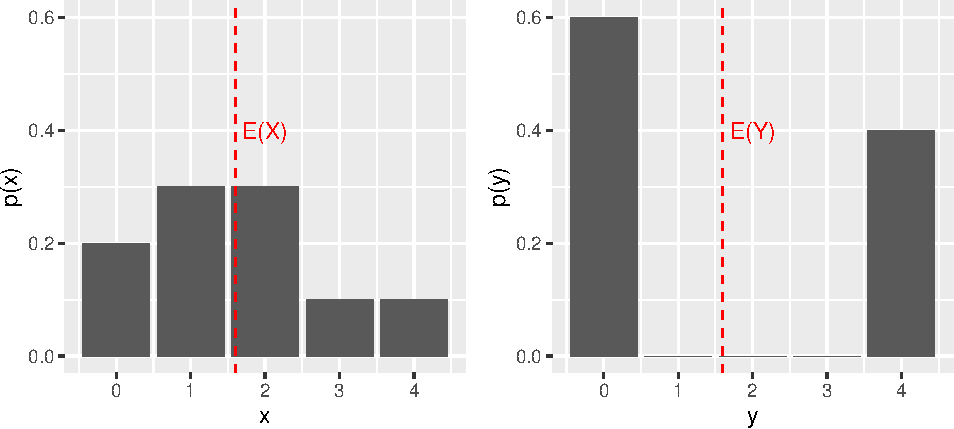
\includegraphics[keepaspectratio]{math340-notes_files/figure-latex/unnamed-chunk-10-1.pdf}}
\end{example}

\begin{example}[Infinite Variance?]
\protect\hypertarget{exm:infinite-variance}{}\label{exm:infinite-variance}There exist discrete random variables with finite mean and infinite variance. Here's one: Recall that the \(p\)-series \[\sum_{n=1}^\infty \frac{1}{n^p}\] converges for \(p > 1,\) and diverges when \(p = 1\). Let's suppose the series \[\sum_{n=1}^\infty \frac{1}{n^3} = c.\]
(In fact, \(c\) equals a known constant close to 1.2, called Apery's constant after the mathematician who proved this constant is irrational.) Consider the discrete random variable \(X\) whose distribution function is given by \[p(x) = \frac{1}{cx^3} ~\text{ for }~ x = 1, 2, 3, \ldots.\]
Then,
\begin{align*}
E(X) &= \sum_{x=1}^\infty x \cdot \frac{1}{cx^3}\\
    &= \frac{1}{c} \sum_{x=1}^\infty \frac{1}{x^2} \\
    &= \frac{\pi^2}{6c},
\end{align*}
since the \(p\)-series \(\sum_{n=1}^\infty (1/n^2) = \pi^2/6.\) So, \(E(X)\) exists as a finite number.

However,
\begin{align*}
E(X^2) &= \sum_{x=1}^\infty x^2 \cdot \frac{1}{cx^3}\\
    &= \frac{1}{c} \sum_{x=1}^\infty \frac{1}{x},
\end{align*}
which diverges as a multiple of the harmonic series. So, \(V(X)\) does not exist as a finite number.
\end{example}

\section{Properties of Expected Value}\label{properties-of-expected-value}

\begin{theorem}
\protect\hypertarget{thm:EV-properties-discrete}{}\label{thm:EV-properties-discrete}

Suppose \(X\) is a discrete random variable, \(c \in \mathbb{R}\) is a constant, and \(g,\) \(g_1,\) and \(g_2\) are functions of \(X\).

\begin{enumerate}
\def\labelenumi{\arabic{enumi}.}
\tightlist
\item
  \(E(c) = c\).
\item
  \(E(c\cdot g(X))= cE(g(X))\).
\item
  \(E(g_1(X) \pm g_2(X)) = E(g_1(X))\pm E(g_2(X))\).
\end{enumerate}

\end{theorem}

These properties can help us evaluate expected values without having to sum over all \(x\).

For instance, suppose we know \(X\) is a discrete random variable with expected value \(E(X) = 1.6\).

Then

\begin{align*}
E(4+3X) &= E(4) + E(3X) &\text{ by property 3} \\
        &= 4 + 3E(X) &\text{ by properties 1 and 2}\\
        &= 4 + 3 \cdot 1.6 &\text { since }E(X) = 1.6 \\
        &= 8.8. &\text{ Nice.}
\end{align*}

Let's take the time to prove these properties. Each of them essentially follows by properties of summations.

\begin{proof}
\leavevmode

\begin{enumerate}
\def\labelenumi{\arabic{enumi}.}
\tightlist
\item
  Given a constant \(c,\) we can view this constant as a function of \(X,\) say \(f(x) = c\). Then
  \begin{align*}
  E(c) &= \sum_{\text{all }x} c \cdot p(x) \\
  &= c \sum_{\text{all }x} p(x)
  \end{align*}
\end{enumerate}

Since the sum over all \(x\) of \(p(x)\) is 1 for any probability model, the result follows.

\begin{enumerate}
\def\labelenumi{\arabic{enumi}.}
\setcounter{enumi}{1}
\item
  Here appeal to Theorem \ref{thm:EV-discrete-fcnRV} and arithmetic:
  \begin{align*}
  E(c\cdot g(X)) &= \sum_{\text{all }x} c \cdot g(x) \cdot p(x) & \\
  &= c \sum_{\text{all }x} g(x) p(x) &\text{by arithmetic}\\
  &= c E(g(X)) & 
  \end{align*}
\item
  Here we also appeal to Theorem \ref{thm:EV-discrete-fcnRV} and arithmetic:
  \begin{align*}
  E(g_1(x) \pm g_2(x)) &= \sum_{\text{all }x} (g_1(x) \pm g_2(x))\cdot p(x) &\\
  &= \sum_{\text{all }x} (g_1(x) p(x) \pm g_2(x) p(x)) &\text{by arithmetic}\\
  &= \sum_{\text{all }x} g_1(x) p(x) \pm \sum_{\text{all }x} g_2(x) p(x)  &\text{by arithmetic}\\
  &= E(g_1(X)) \pm E(g_2(X)) & 
  \end{align*}
\end{enumerate}

\end{proof}

\begin{example}
\protect\hypertarget{exm:homes-near-firehouse}{}\label{exm:homes-near-firehouse}The number \(N\) of residential homes that a fire company can serve depends on the distance \(r\) (in city blocks) that a fire engine can cover in a fixed period of time. If we assume that \(N\) is proportional to the area of a circle \(R\) blocks from the fire house, then \[N = k \pi R^2,\] where \(k\) is a constant, and \(R\) is a random variable. For a particular fire company, \(k = 8,\) and the probability function for \(R\) is
\[
\begin{array}{c|c|c|c|c|c|c|c}
r    &  21 &  22 &  23 &  24 & 25 & 26 \\ \hline
p(r) & .05 & .20 & .30 & .25 & .15 & .05
\end{array}
\]
Find \(E(N),\) the expected number of homes that the fire department can serve.

Well, \[E(N) = E(8\pi R^2) = 8\pi E(R^2),\]
so
\begin{align*}
E(N) &= 8\pi\left(21^2\cdot .05 + 22^2 \cdot .20 + 23^2 \cdot .30 + 24^2 \cdot .25 + 25^2 \cdot .15 + 26^2 \cdot .05\right) \\
&= 8\pi(549.1) \\
&\approx 13,800 \text{ homes}
\end{align*}
\end{example}

\begin{theorem}[Useful Variance Formula]
\protect\hypertarget{thm:variance-shortcut}{}\label{thm:variance-shortcut}Let \(X\) be a discrete random variable with probability function \(p(x)\) and expected value \(E(X) = \mu\). Then \[V(X) = E(X^2)-\mu^2.\]
\end{theorem}

\begin{proof}
By definition,
\begin{align*}
V(X) &= E((X-\mu)^2)\\
     &= E(X^2 - 2\mu X + \mu^2) &\text{by expanding}\\
     &= E(X^2) - E(2\mu X) + E(\mu^2) &\text{by E() Property 3} \\ 
     &= E(X^2) - 2\mu E(X) + \mu^2 &\text{by E() Properties 2 and 1}\\
     &= E(X^2) - 2\mu^2 + \mu^2 & \text{since }E(X)=\mu \\
V(X) &= E(X^2) - \mu^2.
\end{align*}
\end{proof}

This alternate formula for variance also provides us with a way to compute \(E(X^2)\) from the expected value and variance of a random variable: \[E(X^2) = V(X) + \mu^2,\] or using the alternate variance notation:
\[E(X^2) = \sigma^2 + \mu^2.\]

\begin{example}
Suppose \(X\) is a discrete random variable with expected value \(\mu = 5\) and variance \(\sigma^2 = 6\).
Find \(E(3+2X+4X^2)\).

Well, \begin{align*}
E(3 + 2X + 4X^2) &= E(3) + 2E(X) + 4E(X^2) \\
                 &= 3 + 2\cdot \mu + 4[\sigma^2+\mu^2] \\
                 &= 3 + 2 \cdot 5 + 4[6 + 5^2] \\
                 &= 3 + 10 + 124 \\
                 &= 137.
\end{align*}
\end{example}

\section{Tchebysheff's Theorem}\label{tchebysheffs-theorem}

\begin{theorem}[Tchebysheff's Inequality]
\protect\hypertarget{thm:tcheby}{}\label{thm:tcheby}Let \(X\) be a random variable with mean \(E(X) = \mu\) and finite variance \(V(X) = \sigma^2 > 0\). Then for any constant \(k > 0,\)
\[P(|X - \mu| < k\sigma ) \geq 1 - \frac{1}{k^2}.\]\index{Tchebysheff's Inequality}
Equivalently, \[P(|X - \mu| \geq k\sigma) \leq \frac{1}{k^2}.\]
\end{theorem}

For instance, if \(k = 2,\) Tchebysheff's inequality says that for any random variable \(X,\) the probability that \(X\) takes a value that is within 2 standard deviations of the mean is at least .75. For many distributions, this proability is closer to .95, but .75 holds for \emph{all} distributions.
Of course, letting \(k = 1\) in Tchebysheff's inequality gives us the trivially true statement that the probability that \(X\) takes a value within 1 standard deviation of the mean is at least 0.

\begin{proof}
We prove Tchebysheff's inequality in the case for a discrete random variable, and we come back to this theorem after defining continuous random variables.

Let \(k > 0\) be given.

Then \[V(X) = \sum_{\text{all }x} (x - \mu)^2 p(x),\] by the definition of variance. We can partition the space of \(X\) into three disjoint sets, depending on the location of \(x\) relative to \(\mu \pm k\sigma\):

\[V(X) = \sum_{\text{all } x \leq \mu - k\sigma} (x - \mu)^2 p(x) + 
\sum_{\text{all } x \text{ s.t. } |x-\mu|< k\sigma } (x - \mu)^2 p(x) + \sum_{\text{all } x \geq \mu + k\sigma} (x - \mu)^2 p(x)\]

Each of these three sums is non-negative, and for the first and third sums we can also say that \((x-\mu)^2 \geq k^2\sigma^2\) for all \(x\) in the given range, so it follows that \[V(x) \geq \sum_{\text{all } x \leq \mu - k\sigma} k^2\sigma^2 p(x) + 0 + \sum_{\text{all } x \geq \mu + k\sigma} k^2\sigma^2 p(x).\]
So,

\begin{align*}
\sigma^2 &\geq \sum_{\text{all } x \leq \mu - k\sigma} k^2\sigma^2 p(x) + 0 + \sum_{\text{all } x \geq \mu + k\sigma} k^2\sigma^2 p(x)  \\
  &= k^2\sigma^2 \left(\sum_{\text{all } x \leq \mu - k\sigma} p(x) + \sum_{\text{all } x \geq \mu + k\sigma} p(x) \right) \\
  &= k^2\sigma^2\left(P(X\leq \mu-k\sigma)+P(X \geq \mu+k\sigma)\right) \\
  &= k^2\sigma^2P(|X-\mu|\geq k\sigma)
\end{align*}

Dividing both sides of the inequality by the positive value \(k^2\sigma^2\) gives us the result:
\[P(|X-\mu| \geq k\sigma) \leq \frac{1}{k^2}.\]
\end{proof}

\begin{example}
\protect\hypertarget{exm:tcheby}{}\label{exm:tcheby}Suppose \(X\) is a random variable with \(E(X) = 70\) and \(V(X) = 25,\) so \(\mu = 70\) and \(\sigma = \sqrt{25} = 5\).
According to Tchebysheff's inequality with \(k = 2,\) the probability that \(X\) takes a value between 60 and 80 is at least 3/4. Setting \(k = 3,\) we find the probability that \(X\) takes a value between 55 and 85 is at least 8/9.
\end{example}

Again, for many distributions, the probability of being within 2 standard deviations of the mean is much higher than .75 (often about .95, in fact), and the probability of being within 3 standard deviations of the mean is much higher than 8/9 (often about .99).

Here's a distribution, however, that shows the bound in Tchebysheff's inequality cannot be improved.

\begin{example}
\protect\hypertarget{exm:tcheby-best-bound}{}\label{exm:tcheby-best-bound}We show that there exists a probability distribution for which \(P(|X-\mu|<2\sigma) = .75\).

Consider the discrete random variable \(X\) whose probability distribution function is

\[
\begin{array}{c|c|c|c}
x   &  -1 &  0 &  1   \\ \hline
p(x) & .125 & .75 & .125 
\end{array}
\]
Then \[\mu = E(X) = (-1)(.125) + (0)(.75) + (1)(.125) = 0,\] and

\begin{align*}
\sigma^2 &= E(X^2)-\mu^2 \\
  &= (-1)^2(.125) + 0^2(.75) + 1^2(.125)\\
  &=.25,
\end{align*}
So, \(\sigma = 0.5,\) and
\begin{align*}
P(|X - \mu| < 2 \sigma) &= P(|X| < 1) \\
&= P(-1 < X < 1) \\
&= P(X = 0) & \text{ since the space of $X$ is } \{-1,0,1\} \\
&= .75.
\end{align*}

Thus, there exists a discrete random variable for which \(P(|X - \mu| < 2 \sigma) = .75\). In fact, for any \(k > 0\) the probability distribution given by
\[
\begin{array}{c|c|c|c}
x   &  -1 &  0 &  1   \\ \hline
p(x) & \frac{1}{2k^2} & 1-\frac{1}{k^2} & \frac{1}{2k^2} 
\end{array}
\]
will satisfy \(P(|X-\mu|<2\sigma)=1-\frac{1}{k^2},\) demonstrating that the bound in Tchebysheff's inequality can not be increased.
\end{example}

\chapter{Important Discrete Random Variables}\label{important-discrete-rv}

In this chapter we introduce the following well-known discrete random variables:
binomial, geometric, Poisson, negative binomial, and hypergeometric.
In examples we work through, it will from time to time be convenient to compute probabilities in R. Appendix \ref{R-discreteRV} contains details about the commands in R useful for doing so.

\section{Binomial Distributions}\label{binomial}

It all begins with a Bernoulli trial.

\begin{definition}
\protect\hypertarget{def:bernoulli-trial}{}\label{def:bernoulli-trial}A \textbf{Bernoulli trial}\index{Bernoulli trial} is a chance experiment with two distinct possible outcomes, ``success'' and ``failure''. Typically, we let \(p\) denote the probability of success, and \(q\) denote the probability of failure (where \(q = 1 - p\)).
\end{definition}

Some examples:

\begin{enumerate}
\def\labelenumi{\arabic{enumi}.}
\tightlist
\item
  Roll a 6-sided die and define success to be ``roll a 4'', and failure to be ``don't roll a 4''. Here \(p = 1/6\) and \(q = 5/6\).
\item
  Pick a name out of a hat with \(n\) names. Success: pick Oriana's name; Failure: do not pick Oriana's name. Here \(p = 1/n\) and \(q = (n-1)/n\).
\item
  Test a person for a particular disease. In medical tests such as these, ``success'' is often used to describe a positive test (meaning the person tests positive for the disease), and ``failure'' means the person tests negative for the disease.
\end{enumerate}

\begin{definition}[Binomial Distribution]
\protect\hypertarget{def:binomial-distribution}{}\label{def:binomial-distribution}Define the random variable \(X\) to equal the number of successes in \(n\) independent, identical Bernoulli trials with probability of success on any given trial equal to \(p\). Then \(X\) is called a \textbf{binomial distribution with parameters \(n\) and \(p\)}\index{discrete random variable!binomial}, and \(X\) is denoted \(\texttt{binom}(n,p)\)\index{\texttt{binom}$(n,p)$}.

The space of \(X\) equals \(\{0,1,\ldots,n\},\) and for \(x = 0,1, \ldots, n,\)
\[p(x) = \binom{n}{x}p^x(1-p)^{n-x}.\]
\end{definition}

Does this probability distribution make sense? To find the probability of exactly \(x\) successes in \(n\) independent Bernoulli trials, we first choose which \(x\) of the \(n\) trials will be successes (and we have \(\binom{n}{x}\) choices here). Then, we know the probability of success on each of these \(x\) trials is \(p,\) and the probability of failure on each of the other \(n-x\) trials is \(q = 1-p\). Since the trials are independent, the probability of getting exactly \(x\) successes and \(n-x\) failures is the product \(\binom{n}{x}p^x(1-p)^{n-x}.\)

Furthermore, by the Binomial Theorem (\ref{thm:Cnrfacts}), \[\sum_{x = 0}^n p(x) = (p+(1-p))^n = 1.\]

\begin{theorem}
\protect\hypertarget{thm:binomial-distribution-EandV}{}\label{thm:binomial-distribution-EandV}If \(X\) is \(\texttt{binom}(n,p),\) \[E(X) = np~~~\text{ and }~~~ V(X) = np(1-p).\]
\end{theorem}

\begin{proof}
From the definition of expected value,

\begin{align*}
E(X) &= \sum_{x=0}^n x \cdot p(x) \\
     &= \sum_{x=1}^n x \cdot p(x) & \text{since the } x = 0 \text{ term is  } 0 \\
     &= \sum_{x=1}^n x \binom{n}{x} p^x (1-p)^{n-x} \\
     &= \sum_{x=1}^n x \frac{n!}{(n-x)!x!} p^x (1-p)^{n-x} \\
     &= \sum_{x=1}^n \frac{n!}{(n-x)!(x-1)!} p^x (1-p)^{n-x} &\text{cancelling an } x\\
     &= np \sum_{x=1}^n \frac{(n-1)!}{(n-x)!(x-1)!}p^{x-1}(1-p)^{n-x} &\text{ pull out }n\text{ from }n!\text{ and one }p\\
     &= np \sum_{x=1}^n \binom{n-1}{x-1}p^{x-1}(1-p)^{(n-1)-(x-1)}
\end{align*}

Hey! The summation term equals 1 since it is the sum of all the probabilities in a \(\texttt{binom}(n-1,p)\) distrtibution!

Thus \(E(X) = np\).

To prove the \(V(X)\) formula, it is helpful to first observe the following

\[E(X(X-1)) = E(X^2-X) = E(X^2)-E(X),\] so
\[E(X^2) = E(X(X-1))+E(X).\]
We computed \(E(X)\) above, and \(E(X(X-1))\) can be determined similarly:

\begin{align*}
E(X(X-1)) &= \sum_{x=0}^n x(x-1)\binom{n}{x}p^x(1-p)^{n-x} \\
          &= \sum_{x=2}^n x(x-1)\binom{n}{x}p^x(1-p)^{n-x} \\
          &= \sum_{x=2}^n x(x-1)\frac{n!}{(n-x)!x!}p^x(1-p)^{n-x} \\
          &= \sum_{x=2}^n \frac{n!}{(n-x)!(x-2)!}p^x(1-p)^{n-x} \\
          &= n(n-1)p^2 \sum_{x=2}^n \frac{(n-2)!}{(n-x)!(x-2)!}p^{x-2}(1-p)^{n-x} \\
          &= n(n-1)p^2 \sum_{x=2}^n\binom{n-2}{x-2}p^{x-2}(1-p)^{(n-2)-(x-2)}
\end{align*}

This summation also equals one, since it is the sum of all the probabilities in a \(\texttt{binom}(n-2,p)\) distribution, so \(E(X(X-1)) = n(n-1)p^2,\) and it follows that
\[E(X^2) = E(X(X-1))+E(X) = n(n-1)p^2 + np.\]

Finally,
\begin{align*} 
V(X) &= E(X^2) - E(X)^2 \\
     &= n(n-1)p^2 + np - (np)^2 \\
     &= n^2p^2 - np^2 + np - n^2p^2 \\
     &= np(1-p)
\end{align*}
\end{proof}

\begin{example}[Guessing on a multiple choice test]
\protect\hypertarget{exm:binom-mult-choice-test}{}\label{exm:binom-mult-choice-test}A multiple choice exam has 15 questions. Each question has 4 possible answers. If a student answers each question with a random guess, what is the probability they will score 10 or higher?

Let \(X\) = the score on the test. Then, \(X\) is \(\texttt{binom}(n=15,p=1/4)\).

Now, \[P(X \geq 10) = \sum_{x = 10}^{15} \binom{15}{x}\left(\frac{1}{4}\right)^x\left(\frac{3}{4}\right)^{15-x} \approx .0008.\]

\textbf{Calculating this sum in R}

R has a nice command for calculating cumulative probabilities of the form \(P(X \leq x)\).If \(X\) is \(\texttt{binom}(n,p),\) then \(P(X \leq x)\) is calculated in R by \texttt{pbinom(x,n,p)}. So, in the case of the multiple choice test, \(P(X \geq 10) = 1 - P(X \leq 9) =\) \texttt{1-pbinom(9,15,1/4)}. See Appendix \ref{R-discreteRV}) for more information on using R to calculate probabilities for the important discrete distributions we encounter in this class.

Back to the test, they have less than a 1 in a thousand chance of scoring a 10 or better if they are truly guessing. Note also that the mean for \(X\) is \(E(X) = 15 \cdot \frac{1}{4} = 3.75\).

What if they can eliminate one of the choices on each problem, and randomly guess between the remaining three choices on each problem? Are they likely to do better? If we let \(Y\) denote the score on the test following this approach, then \(Y\) is \(\texttt{binom}(n=15,p=1/3),\) and the probability of scoring 10 or greater ends up about 10 times better than it was before, but still miniscule:

\[P(Y \geq 10) = \sum_{y = 10}^{15} \binom{15}{y}\left(\frac{1}{3}\right)^y\left(\frac{2}{3}\right)^{15-y} \approx .0085,\]
The mean score is now \(E(Y) = 15\cdot\frac{1}{3} = 5.\) Ok, not great, but it is better, I guess.
\end{example}

\begin{example}[Pay the meter?]
\protect\hypertarget{exm:parking-meter}{}\label{exm:parking-meter}This example is adapted from an exercise in the Grinstead-Snell text. Flint never puts money in a 25-cent parking meter downtown. He assumes that there is a probability of .03 that he will be caught. The first offense costs nothing, the second costs 10 dollars, and subsequent offenses cost 25 dollars each.

\begin{quote}
How does the expected cost of parking 100 times without paying the meter compare with the cost of paying the meter each time?
\end{quote}

Assume parking events are independent, identical Bernoulli trials with probability \(p = .03\) of getting a ticket. Then the random variable \(X\) counting the number of tickets in 100 trials is \(\texttt{binom}(100,.03),\) and we note that \(E(X) = 100\cdot(.03) = 3\).

In deciding whether to pay the meter, one idea is to consider the cost associated to the expected number of tickets, which would be \$35. This amount is higher than the \$25 Flint would pay by chucking in a quarter each time. But this approach doesn't give the full picture.

Instead, let's determine the expected cost associated to parking 100 times without paying the meter. If Flint never pays the meter, the parking cost \(C\) of these 100 trials is the following function of \(X\):

\[
C(x)=
\begin{cases}
0 &\text{ if }x = 0,1 \\
10  &\text{ if } x = 2 \\
10+25(x-2) &\text{ if } x \geq 3 
\end{cases}
\]

Then the expected cost associated with these 100 trials, \(E(C),\) is
\begin{align*}
E(C) &= \sum_{x=0}^{100} C(x)\cdot p(x)\\
    &= C(2)\cdot p(2) + \sum_{x=3}^{100} (10 + 25\cdot(x-2))\cdot p(x) \\
    &= 10\cdot p(2) + \sum_{x=3}^{100} (25x - 40)\cdot p(x) \\
    &= 10\cdot p(2)  + \left(E(25X-40) - \sum_{x=0}^{2} (25x - 40)\cdot p(x)\right)\\
    &= 10\cdot p(2) + [25\cdot E(X) - 40] - \left(-40\cdot p(0) -15 \cdot p(1)+ 10*p(2)\right)\\
    &= [25 E(X) - 40] + 40 \cdot p(0) + 15 \cdot p(1) \\
    &= [(25 \cdot 3) - 40] + 40\cdot(.97)^{100} + 15\cdot 100(.03)(.97)^{99} \\
    &\approx 39.10.
\end{align*}

Yes, Flint is better off putting a quarter in the meter each time for a cost of \$25 in parking. But never tell Flint the odds.
\end{example}

\begin{example}[Drilling for Oil]
\protect\hypertarget{exm:binomial-oil}{}\label{exm:binomial-oil}An oil exploration firm in the 1970s wants to finance 10 drilling explorations. They figure each exploration has a probability of success (finding oil) equal to 0.1, and that the 10 operations are independent (success in one is independent of success in any other). The company has \$50,000 in fixed costs prior to doing its first exploration, and anticipates a cost of \$150,000 for each unsuccessful exploration, and a cost of \$300,000 for each successful exploration. Find the expected total cost to the firm for its 10 explorations.

Let \(X\) = number of successful explorations. Then \(X\) is \(\texttt{binom}(10,.1),\) and \(E(X) = 10 \cdot .1 = 1.\)
The cost \(C\) (in thousands of dollars) can be expressed as a linear function of \(X\):

\begin{align*}
C &= 50 + 150(10-X)+300X\\
  &= 1550 + 150X.
\end{align*}

It follows from properties of expected value that
\begin{align*}
E(C) &= E(1550 + 150X)\\
     &= E(1550) + 150E(X)\\
     &= 1550 + 150 \cdot 1 \\
     &= 1700.
\end{align*}
So the expected cost is \$1.7 million dollars.
\end{example}

\begin{example}[AI Generated Example]
\protect\hypertarget{exm:binomial-AI-generated}{}\label{exm:binomial-AI-generated}In a galaxy not so far away, there is a soccer ball factory run by enthusiastic, if somewhat clumsy, aliens. The factory manager, Zorg, claims that only 5\% of the soccer balls they produce end up being ``special'' (read: defective). The company's quality control inspector, an alien named Blurp, is highly skeptical and decides to randomly select 20 soccer balls from a day's production to test this claim.

\textbf{Questions}:

\begin{enumerate}
\def\labelenumi{\arabic{enumi}.}
\tightlist
\item
  If Zorg's claim is correct, what is the probability that exactly 2 of the 20 selected soccer balls are ``special''?
\item
  If Zorg's claim is correct, what is the probability that at most 1 of the 20 selected soccer balls is ``special''?
\item
  If Zorg's claim is correct, what is the probability that more than 3 of the 20 selected soccer balls are ``special''?
\end{enumerate}

\textbf{Solution}:

Let \(X\) denote the number of ``special'' soccer balls in the randomly selected set of 20 balls. Then, \(X\) is \(\texttt{binom}(n=20,p=.05)\)

The first question asks for \(P(X = 2)\) which is \[P(X = 2) = \binom{20}{2} p^2 \cdot (1-p)^{18} \approx .189.\]

The second question asks for \[P(X \leq 1) = \sum_{x = 0}^1 \binom{20}{x}p^x(1-p)^{20-x},\]
and using R, we see that \(P(X \leq 1)\) = \texttt{pbinom(1,20,.05)} \(\approx\) 0.736.

The third question asks for \[P(X > 3) = 1 - P(X \leq 3),\]
which we can evaluate in R with
\texttt{1-pbinom(3,20,.05)} \(\approx\) 0.016.
\end{example}

\begin{example}
\protect\hypertarget{exm:binomial-tchebby}{}\label{exm:binomial-tchebby}

Suppose \(X\) is \(\texttt{binom}(60,1/4)\). Then \(\mu = 60\cdot\frac{1}{4} = 15\) and \(\sigma^2 = 60\cdot \frac{1}{4} \cdot \frac{3}{4} = 11.25.\)
Tchebbysheff says at least 75\% of the distribution is within 2 standard deviations of the mean, so in this case, at least 75\% of the distribution is between \(15 - 2\cdot \sqrt{11.25}\) and \(15 + 2\cdot \sqrt{11.25},\) or between 8.3 and 21.7. The actual percentage is closer to 95\%, and it can be found by summing all \(p(x)\) for \(x\) between 8.29 and 21.7. This sum is calculated in R by

\begin{Shaded}
\begin{Highlighting}[]
\FunctionTok{pbinom}\NormalTok{(}\FloatTok{21.7}\NormalTok{,}\DecValTok{60}\NormalTok{,}\DecValTok{1}\SpecialCharTok{/}\DecValTok{4}\NormalTok{)}\SpecialCharTok{{-}}\FunctionTok{pbinom}\NormalTok{(}\FloatTok{8.29}\NormalTok{,}\DecValTok{60}\NormalTok{,}\DecValTok{1}\SpecialCharTok{/}\DecValTok{4}\NormalTok{)}
\end{Highlighting}
\end{Shaded}

\begin{verbatim}
## [1] 0.9489842
\end{verbatim}

\end{example}

\section{Geometric Distributions}\label{geometric}

Suppose we have a sequence of Bernoulli trials, independent, with probability of success \(p\) on each trial. Let \(X\) equal the number of trials up to and including the trial of the first success. Then \(X\) is called a \textbf{geometric distribution with parameter \(p\)}\index{discrete random variable!geometric}, denoted \(\texttt{geom}(p)\)\index{\texttt{geom}$(p)$}.

The probability function for \(X\) is given by \[p(x) = q^{x-1}\cdot p,\] for \(x = 1, 2, 3, \ldots,\) where, again, \(q = 1-p\).

Note that \[\sum_{x=0}^\infty p(x) = p + pq + pq^2 + \cdots\] is a geometric series with \(|q| < 1\) so it converges. Moreover, by the geometric series formula\index{geometric series formula}, \[\sum_{n=0}^\infty pq^n = \frac{p}{1-q}.\]
Thus, all the \(p(x)\) sum to 1, and we have a valid probability function.

More generally, for any non-negative integer \(k,\)
\begin{align*}
P(X > k) &= p(X=k+1)+p(X=k+2)+p(X=k+3)+\cdots \\
        &= pq^k + pq^{k+1}+pq^{k+2}+\cdots \\
        &= pq^k(1 + q + q^2 + \cdots)\\
        &= pq^k\cdot\frac{1}{1-q}\\
        &= q^k.
\end{align*}

The geometric distribution can be useful when modeling the behavior of lines. For instance, suppose a line of cars waits to pay their parking fee as they exit the airport. It can be reasonable to assume that over a short interval of time (say 10 seconds), the probability that a car arrives is \(p,\) and the probability that a car does not arrive is \(q = 1-p.\) Then the time \(T\) until the next arrival has a geometric distribution, and by the remark above, the probability that no car arrives in the next \(k\) time units is \(P(T > k) = q^k\).

\begin{theorem}
\protect\hypertarget{thm:geometric-EandV}{}\label{thm:geometric-EandV}If \(X\) is \(\texttt{geom}(p)\) for \(0 < p \leq 1,\) then \[E(X) = \frac{1}{p}~~~\text{ and }~~~  V(X) = \frac{1-p}{p^2}.\]
\end{theorem}

Before proving this theorem we consider the geometric series one more time.

\emph{Geometric Series Intermission}

From Calc II we know that the geometric series \(\sum q^x\) converges if and only if \(-1 < q < 1,\) and that \[\sum_{x = 0}^\infty q^x=\frac{1}{1-q} \tag{provided |q|<1}\] Thinking of \(q\) as a variable, we can differentiate each side with respect to \(q,\) and the resulting infinite series will still converge for \(-1 < q < 1\).

\begin{align*}
\frac{d}{dq}\left[\sum_{x = 0}^\infty q^x\right] &= \frac{d}{dq}\left[\frac{1}{1-q}\right] \\
\frac{d}{dq}\left[1+q+q^2 + q^3 + \cdots \right] &= \frac{d}{dq}\left[\frac{1}{1-q}\right] \\
\left[0 + 1 + 2q + 3q^2 + \cdots\right] &= \frac{1}{(1-q)^2}\\
\sum_{x = 1}^\infty x q^{x-1} &= \frac{1}{(1-q)^2}.
\end{align*}

\emph{This ends the geometric series intermission.}

\begin{proof}
By definition of expected value,
\begin{align*}
E(X) &= \sum_{x=1}^\infty x \cdot q^{x-1}\cdot p \\
&= p \sum_{x=1}^\infty x \cdot q^{x-1}.
\end{align*}
But this series is exactly the one for which we found a formula in the intermission above, so \[E(X) = p \cdot \frac{1}{(1-q)^2} = \frac{1}{p}.\]

We leave the proof that \(V(X) = \frac{1-p}{p^2}\) as an exercise.
\end{proof}

\begin{example}[Message Received]
\leavevmode

\begin{quote}
Assume that, during each second, my junk box receives one email with probability .01 and no email with probability .99. Determine the probability that I will not receive a junk email in the next 10 minutes.
\end{quote}

We let \(X\) count how many seconds (from now) it takes to be sent an email to my junk box, and we assume \(X\) is \(\texttt{geom}(p = .01)\).

Then the probability of not receiving a junk email in the next ten minutes is \[P(X > 600) = q^{600} \approx .0024.\]
So you're saying there's a chance!

We also note that \(E(X) = 1/p = 100,\) the average time to get our next junk mail is 100 seconds.

\end{example}

\section{Negative Binomial Distribution}\label{negative-binomial}

Suppose we have a sequence of independent Bernoulli trials, each having probability of success \(p,\) and we want to know how many trials it takes to get our \(r\)th success, where \(r \geq 1\).

For instance, if we set \(r = 3,\) then \(X = 7\) for the following sequence of Bernoulli trials (\(S\) stands for success, \(F\) for failure)
\[F F F S F S S F S F F S \ldots \]
since the third \(S\) occurs on the 7th trial.

Let \(X\) equal the number of trials up to and including the trial of the \(r\)th success. Then \(X\) is called a \textbf{negative binomial distribution with parameters \(r\) and \(p\)}\index{discrete random variable!negative binomial}, denoted \(\texttt{nbinom}(r,p)\)\index{\texttt{nbinom}$(r,p)$}.

The space of \(X\) is \(\{r, r+1, r+2, \ldots\}\) and for \(x\) in the space of \(X\) the probability function for \(X\) is given by \[p(x) = \binom{x-1}{r-1}p^r(1-p)^{x-r}.\]

Note, that if \(r=1\) we just have the friendly geometric distribution.

\begin{theorem}
\protect\hypertarget{thm:negative-binomial-EandV}{}\label{thm:negative-binomial-EandV}If \(X\) is \(\texttt{nbinom}(r,p)\) where \(0 < p \leq 1\) then
\[E(X) = \frac{r}{p} ~~~ \text{ and } ~~~ V(X) = \frac{r(1-p)}{p^2}.\]
\end{theorem}

\begin{example}
\leavevmode

\begin{quote}
If we roll 2 dice and record the sum, how many rolls, on average, will it take to get our 4th 8?
\end{quote}

Well, the probability of rolling a sum of 8 is \(p = 5/36\) by our 6x6 dice grid in Example \ref{exm:roll2dice}, and the random variable \(X\) counting the number of rolls until we get our 4th 8 is \(\texttt{nbinom}(r=4,p=5/36),\) so \[E(X) = \frac{4}{5/36} = 28.8.\] Would you want to make a bet that it will take me more than 25 rolls to get my 4th 8?

We note that \[V(X) = \frac{4\cdot (31/36)}{(5/36)^2} \approx 178.6,\] so the standard deviation is \(\sigma = \sqrt{V(X)} \approx 13.36\).

\end{example}

\section{Hypergeometric Distribution}\label{hypergometric}

Here's the scene: We have a finite population with \(N\) total elements, and this population can be partitioned into two distinct groups, where

\begin{itemize}
\tightlist
\item
  group 1 has \(m\) elements, and
\item
  group 2 has \(n\) elements, (so \(m + n = N\)).
\end{itemize}

Think: a box of \(N\) marbles, \(m\) of them are orange and \(n\) of them are green.

Suppose we draw a random sample without replacement of size \(k\) from the population.

Let \(X\) equal the number of elements in the sample of size \(k\) that belong to group 1.

Then \(X\) is called a \textbf{hypergeometric distribution with parameters \(m, n,\) and \(k\)}\index{discrete random variable!hypergometric}, denoted \(\texttt{hyper}(m,n,k)\)\index{\texttt{hyper}$(m,n,k)$}. The space of \(X\) is either
\(x = 0, 1, \ldots, k\) if \(m \geq k,\) or \(0, 1, \ldots, m\) if \(m < k\).

For each \(x\) in the space of \(X,\)
\[p(x) = \frac{\binom{m}{x}\binom{n}{k-x}}{\binom{N}{k}},\] where \(N = m + n\).

The classic ``good potatoes/bad potatoes'' Example \ref{exm:potatoes} has a hypergeometric distribution.

\begin{theorem}
\protect\hypertarget{thm:hypergeometric-EandV}{}\label{thm:hypergeometric-EandV}If \(X\) is \(\texttt{hyper}(m,n,k)\) then \[E(X) = k\cdot\frac{m}{N}~~~\text{ and }~~~ V(X) = k \left(\frac{m}{N}\right)\left(\frac{n}{N}\right)\left(\frac{N-k}{N-1}\right),\] where \(N = m + n\).
\end{theorem}

\begin{example}
\protect\hypertarget{exm:hyper-skittles}{}\label{exm:hyper-skittles}\leavevmode

\begin{quote}
Let's say a bag of 120 skittles has 30 orange ones. If we pick 10 at random, what is the probability that we get more than 5 orange ones?
\end{quote}

Let \(X\) denote the number of orange skittles in our sample. Then \(X\) is \(\texttt{hyper}(30,90,10),\) and
\[P(X>5) = \sum_{x=6}^{10} \frac{\binom{30}{x}\binom{90}{10-x}}{\binom{120}{10}} \approx .0153.\]
We note that in this example \(E(X) = 10 \cdot \frac{30}{120} = 2.5.\)

\end{example}

\section{Poisson Distribution}\label{poisson}

\textbf{The Scene}\\
The Poisson probability distribution can provide a good model for the number of occurrences \(X\) of a rare event in time, space, or some other unit of measure. A Poisson random variable \(X\) has one parameter, \(\lambda,\) which is the average number of occurrences of the rare event in the indicated time (or space, etc.)

Some examples that might be well-modeled by a Poisson distribution:

\begin{itemize}
\tightlist
\item
  the number of customers going through a check-out lane in a grocery store per hour;
\item
  the number of typos per page in a book;
\item
  the number of goals scored in a World Cup soccer game;
\item
  the number of chocolate chips per cookie in a big batch;
\item
  the number of pitches per baseball in a baseball game;
\end{itemize}

\begin{definition}[Poisson Distribution]
\protect\hypertarget{def:poisson-distribution}{}\label{def:poisson-distribution}A random variable \(X\) has a \textbf{Poisson probability distribution}\index{discrete random variable!Poisson} with parameter \(\lambda > 0,\) denoted \(\texttt{Poisson}(\lambda)\)\index{\texttt{Poisson}$(\lambda)$}, if and only if \[p(x) = \frac{\lambda^x e^{-\lambda}}{x!} ~~~\text{ for } x = 0,1,2, \ldots.\]
\end{definition}

We take the time to explain how this probability density function does actually model such things, but first let's check that it is a valid probability density function, and then find \(E(X)\) and \(V(X)\).

First, since \(\lambda > 0,\) each \(p(x)\) is non-negative. Also, recall the Calc II power series formula for \(e^\lambda\) for any real number \(\lambda\) is \[e^\lambda = \sum_{k=0}^\infty \frac{\lambda^k}{k!},\] so we can see that all the probabilities in this distribution sum to 1:
\begin{align*}
\sum_{x=0}^\infty \frac{\lambda^x e^{-\lambda}}{x!} &= e^{-\lambda} \sum_{x=0}^\infty \frac{\lambda^x}{x!} \\
&= e^{-\lambda}\cdot e^{\lambda} \\
&= 1.
\end{align*}

\begin{theorem}
\protect\hypertarget{thm:poisson-EandV}{}\label{thm:poisson-EandV}If \(X\) is \(\texttt{Poisson}(\lambda),\) \(E(X) = \lambda\) and \(V(X) = \lambda\).
\end{theorem}

\begin{proof}
We tackle the mean first.

\begin{align*} 
E(X) &= \sum_{x=0}^\infty x \cdot p(x) \\
     &= \sum_{x=1}^\infty x \cdot \frac{\lambda^x e^{-\lambda}}{x!} & \text{since }x=1 \text{ term is } 0\\
     &= e^{-\lambda} \sum_{x=1}^\infty \frac{\lambda^x}{(x-1)!} & \text{since } \frac{x}{x!}=\frac{1}{(x-1)!}\\
     &= \lambda e^{-\lambda} \sum_{x=1}^\infty \frac{\lambda^{x-1}}{(x-1)!} & \text{pulling out one }\lambda \\
     &= \lambda e^{-\lambda} \sum_{k=0}^\infty \frac{\lambda^{k}}{(k)!} & \text{letting }  k = x-1\\
     &= \lambda e^{-\lambda}\cdot e^{\lambda} &\text{power series for }e^\lambda\\
     &= \lambda.
\end{align*}

Thus, \(\mu = \lambda\).

For \(V(X),\) we first find \(E(X(X-1))\) in much the same way as we found \(E(X)\):

\begin{align*}
E(X(X-1)) &= \sum_{x=0}^\infty x(x-1)\cdot \frac{\lambda^x e^{-\lambda}}{x!} \\
    &= e^{-\lambda} \sum_{x=2}^\infty \frac{x(x-1)}{x!} \cdot \lambda^x & \text{since }x=0,1 \text{ terms are }0. \\
    &= e^{-\lambda} \sum_{x=2}^\infty \frac{1}{(x-2)!} \cdot \lambda^x\\
    &= \lambda^2 e^{-\lambda} \sum_{x=2}^\infty \frac{1}{(x-2)!} \cdot \lambda^{x-2}  & \text{pulling out }\lambda^2 \\
    &= \lambda^2 e^{-\lambda} \sum_{k=0}^\infty \frac{1}{(k)!} \cdot \lambda^{k} &\text{letting }k=x-2\\
    &= \lambda^2 e^{-\lambda} \cdot e^{\lambda}  & \text{power series for }e^\lambda\\
    &= \lambda^2.
\end{align*}

Finally, we find \(V(X)\) using our expectation shortcuts:

\begin{align*}
V(X) &= E(X^2) - \mu^2 \\
  &= [E(X(X-1))+E(X)] - \mu^2 \\
  &= [\lambda^2 + \lambda] - \lambda^2 \\
  &= \lambda.
\end{align*}
\end{proof}

\begin{example}
\protect\hypertarget{exm:poisson-typos}{}\label{exm:poisson-typos}Suppose \(X\) gives the number of typos per page in a large printed manuscript, and \(X\) is Poisson with \(\lambda = 2\). Find the probability that a randomly chosen page has (a) fewer than 2 typos, and (b) more than 5 typos.

Part (a) asks for

\begin{align*}
P(X\leq 1) &= P(X = 0)+P(X=1) \\
&= \frac{2^0e^{-2}}{0!}+\frac{2^1e^{-2}}{1!}\\
&= e^{-2} + 2e^{-2} \\
&=3 e^{-2} \\
&\approx 0.406.
\end{align*}

Part (b) asks for

\begin{align*}
P(X >  5) &= 1 - P(X \leq 5) \\
&= 1 - \left[ \frac{2^0e^{-2}}{0!}+\frac{2^1e^{-2}}{1!} +  \cdots + \frac{2^5e^{-2}}{5!}\right]
\end{align*}

Rather than calculate this by hand, we turn to R, and the command \texttt{ppois(k,lambda)}, which returns \(P(X \leq k)\) when \(X\) is \(\texttt{Poisson}(\lambda)\).

So \(P(X > 5) = 1 - P(X \leq 5)\) = 1 - \texttt{ppois(5,2)} \(\approx\) 0.017.
\end{example}

\begin{example}
\protect\hypertarget{exm:pois-website}{}\label{exm:pois-website}The number of website views at a seldom visited website is Poisson with an average number of 8 visits per day.

\begin{quote}
What is the probability that the site gets 20 or more visits in a day?
\end{quote}

We want \(P(X \geq 20),\) an infinite sum, so we use the strategy of finding the complement, with the help of the function \texttt{ppois()} (Appendix \ref{R-discreteRV}) in R for the calculation:

\begin{align*}
P(X \geq 20) &= 1 - P(X \leq 19) \\
&= 1 - \texttt{ppois}(19,8)\\
&\approx .00025.
\end{align*}
\end{example}

\subsection{Poisson Process}\label{poisson-process}

If we're interested in modelling the number of instances of some rare event over a time interval, we can imagine subdividing the interval into \(n\) small pieces, small enough that at most 1 instance can occur in each subinterval. In fact, we can imagine each subinterval constitutes a Bernoulli trial of sorts:

\begin{itemize}
\tightlist
\item
  the probability of 1 instance in a subinterval (``success'') equals \(p\);
\item
  the probability of 0 instances (``failure'') equals \(1-p\).
\end{itemize}

Then, if \(X\) equals the number of instances in the original interval, then \(X\) is binomial on \(n\) trials with probability of success \(p\) on each trial, assuming identical, independent Bernouilli trials. As we increase \(n,\) breaking the original time period into smaller and smaller subintervals, the corresponding probability \(p\) of seeing 1 instance of the event in a subinterval will decrease, but what if \(n \cdot p\) remains constant? In this case, let \(\lambda = np\) and consider what happens to the probability density function for the \(\texttt{binom}(n,p)\) distribution:

\begin{align*}
\lim_{n \to \infty} \binom{n}{x}p^x(1-p)^{n-x} & = \\
\lim_{n \to \infty} \frac{n\cdot(n-1)\cdot \cdots \cdot (n - x + 1)}{x!} \left(\frac{\lambda}{n}\right)^x\left(1-\frac{\lambda}{n}\right)^{n-x} & \\
=\lim_{n \to \infty} \frac{\lambda^x}{x!}\cdot\frac{n\cdot(n-1)\cdot \cdots \cdot (n - x + 1)}{n^x}\cdot\left(1-\frac{\lambda}{n}\right)^{n}\left(1-\frac{\lambda}{n}\right)^{-x}\\
=\frac{\lambda^x}{x!}\lim_{n \to \infty}\left(1-\frac{\lambda}{n}\right)^{n}\left(1-\frac{\lambda}{n}\right)^{-x} \cdot \frac{n}{n} \cdot \frac{n-1}{n} \cdot \frac{n-2}{n} \cdot \cdots \cdot \frac{n-x+1}{n}.
\end{align*}

Now, we have a limit of a product of many terms. If the limit of each term exists, then the overall limit will be the product of each of the individual limits.

First, observe that \((1-\lambda/n)^n \to e^{-\lambda}\) as \(n \to \infty\) by one of the greatest limits in mathematics: \[\lim_{n \to \infty}\left(1+\frac{x}{n}\right)^n = e^x\] for any real number \(x\).

Second, observe that \((1-\lambda/n)^{-x} \to 1^{-x} = 1\) since \(\lambda/n \to 0\) as \(n \to \infty\).

Finally, for any \(k \geq 0,\) \(\lim_{n \to \infty} \frac{n-k}{n} = 1\) so each of the ratios from the third term on converges to 1.

So, if \(np\) remains constant as \(n \to \infty,\) then as \(n \to \infty\) the binomial distribution \(\texttt{binom}(n,p)\) approaches the \(\texttt{Poisson}(\lambda)\) distribution, where \(\lambda = np\). So, the Poisson distribution can be a good model for counting instances of some rare event.

The process described above, where subdivision of the interval leads to Bernoulli trials in such a way that \(np\) remains constant, is called a Poisson process.

\begin{definition}
\protect\hypertarget{def:def-pois-process}{}\label{def:def-pois-process}

The process by which an event happens is called a \textbf{Poisson process}\index{Poisson process} if the following holds:

\begin{enumerate}
\def\labelenumi{\arabic{enumi}.}
\tightlist
\item
  The dimension over which \(X\) is measured can be subdivided into \(n\) small pieces, within which the event can occur \emph{at most once}.
\item
  In each small piece, the probability of seeing one occurrence is the same, say \(p,\) and \(p\) is proportional to the length of the sub-interval (as \(n\) grows, \(p\) shrinks, but \(np\) remains constant).
\item
  Occurrences in all the small pieces are independent from one another.
\end{enumerate}

\end{definition}

In the limit derivation above we demonstrated the following:

\begin{quote}
For large \(n,\) if we let \(\lambda = np,\) \(\texttt{Poisson}(\lambda) \sim  \texttt{binom}(n,p)\).
\end{quote}

For instance, in the table below we compare the probabilities for \(\texttt{binom}(10,.4),\) \(\texttt{binom}(40,.1),\) and \(\texttt{binom}(400,.01)\) with those of a \(\texttt{Poisson}(4)\) distribution:

\begin{table}
\centering
\caption{\label{tab:plot-pois-binom}Approximating a Poisson distn with Binomial distns}
\centering
\begin{tabular}[t]{r|r|r|r|r}
\hline
x & binom(10,.4) & binom(40,.1) & binom(400,.01) & Poisson(4)\\
\hline
0 & 0.0060 & 0.0148 & 0.0180 & 0.0183\\
\hline
1 & 0.0403 & 0.0657 & 0.0725 & 0.0733\\
\hline
2 & 0.1209 & 0.1423 & 0.1462 & 0.1465\\
\hline
3 & 0.2150 & 0.2003 & 0.1959 & 0.1954\\
\hline
4 & 0.2508 & 0.2059 & 0.1964 & 0.1954\\
\hline
5 & 0.2007 & 0.1647 & 0.1571 & 0.1563\\
\hline
6 & 0.1115 & 0.1068 & 0.1045 & 0.1042\\
\hline
7 & 0.0425 & 0.0576 & 0.0594 & 0.0595\\
\hline
\end{tabular}
\end{table}

\begin{example}
\protect\hypertarget{exm:pois-process}{}\label{exm:pois-process}Industrial accidents occur according to a Poisson process with an average of 3 accidents per month. During the last 2 months 10 accidents occurred. Does this number seem highly improbable if the mean number of accidents per month is still equal to 3? Does it indicate a genuine increase in the mean number of accidents per month?

If \(X\) equals the number of accidents in \emph{two} months, then \(X\) is Poisson with mean \(\lambda = 6\).

Then \(P(X \geq 10) = 1 - P(X \leq 9) =\) \texttt{1-ppois(9,6)} = 0.084.

Let's consider this result. If the mean number of accidents per month is still 3, we would expect to observe 10 or more accidents over a two month period about 8 times out of 100, which is unlikely, but not extremely unlikely. Better safe than sorry, I would send out a safety memo and closely monitor what unfolds over the next month!

Now, if we had 5 more accidents the next month, giving us 15 over a 3 month window, chances of 15 or more over 3 months is \(P(X \geq 15),\) where \(X\) is \(\texttt{Poisson}(9)\). Using R, this probability is \texttt{1-ppois(14,9)} = 0.041.

So we have about a 4\% chance of seeing 15 or more over a 3 month window if the mean number of accidents per month is 3. I would investigate whether some practice has changed to make accidents more likely than they used to be.
\end{example}

\begin{example}
\protect\hypertarget{exm:pois-tchebby}{}\label{exm:pois-tchebby}For a certain type of soil the number of wireworms per cubic foot has a Poisson distribution with mean of 100.

\begin{quote}
Give an interval that captures at least 5/9ths of the distribution.
\end{quote}

OK, this feels like a job for Tchebbysheff.

Here \(X\) is Poisson with parameter \(\lambda = 100,\) so \(\mu = 100\) and \(\sigma = \sqrt{100} = 10.\)

Thinking of Tchebbysheff's inequality, let's find \(k\) so that \(1 - 1/k^2 = 5/9\). Then \[P(|X-\mu|<k\sigma)\geq 5/9,\] meaning at least 5/9ths of the distribution is in the interval \((\mu - k\sigma,\mu+k\sigma)\).

Solving
\(1 - \frac{1}{k^2} = \frac{5}{9}\) for \(k>0\) yields \(k = \frac{3}{2},\) so the interval is 85 to 115 wireworms.
\end{example}

\chapter{Moments and Moment-Generating Functions}\label{moments-and-moment-generating-functions}

For random variable \(X\) we have seen that \(E(X)\) and \(E(X^2)\) provide useful information:

\begin{itemize}
\tightlist
\item
  \(\mu = E(X)\) gives the mean of the distribution
\item
  \(\sigma^2 = E(X^2) - E(X)^2\) gives the variance of the distribution.
\end{itemize}

\begin{definition}
\protect\hypertarget{def:kth-moment-about-origin}{}\label{def:kth-moment-about-origin}Let \(X\) be a random variable, and \(k \geq 1\). The \textbf{\(k\)th moment of \(X\) about the origin}\index{moment!about the origin} is \(E(X^k)\). More generally, for any constant \(c \in \mathbb{R},\) \(E((X-c)^k)\) is called the \textbf{\(k\)th moment of \(X\) about \(x = c\)}\index{moment!about $x=c$}.
\end{definition}

Often times we can encode all the moments of a random variable in an object called a moment-generating function.

\begin{definition}
\protect\hypertarget{def:moment-generating-function}{}\label{def:moment-generating-function}Let \(X\) be a discrete random variable with density function \(p(x)\). If there is a positive real number \(h\) such that for all \(t \in (-h,h),\) \[E(e^{tx})\] exists and is finite, then the function of \(t\) defined by \[m(t) = E(e^{tx})\] is called the moment-generating function of \(X\).
\end{definition}

\begin{example}
Suppose \(X\) has the density function
\[
\begin{array}{c|c|c|c|c}
x & 0 & 1 & 2 & 3  \\ \hline
p(x) & .1 & .2 & .3 & .4
\end{array}
\]

Then, for any real number \(t,\)

\begin{align*}
m(t) &= E(e^{tx}) \\
  &= \sum_{x=0}^3 e^{tx}\cdot p(x)\\
  &= e^0\cdot (.1) +e^t\cdot (.2)+e^{2t}\cdot (.3) +e^{3t}\cdot (.4)\\
  &= .1 + .2e^t + .3e^{2t} + .4e^{3t},
\end{align*}

and this sum exists as a finite number for any \(-\infty < t < \infty,\) so the mgf for \(X\) exists.
\end{example}

How does \(m(t)\) \textbf{encode the moments} \(E(X), E(X^2), E(X^3), \ldots\)?

\begin{theorem}[Extracting Moments from the Moment-generating Function]
\protect\hypertarget{thm:mgf}{}\label{thm:mgf}Suppose \(X\) is a random variable with moment-generating function \(m(t)\) which exists for \(t\) in some open interval containing 0. Then the \(k\)th moment of \(X\) equals the \(k\)th derivative of \(m(t)\) evaluated at \(t = 0\):
\[E(X^k) = m^{(k)}(0).\]
\end{theorem}

\begin{proof}
Let's say \(X\) is discrete and \[m(t) = \sum_{\text{all }x} e^{tx}\cdot p(x).\]
Then the derivative of \(m(t)\) with respect to the variable \(t\) is
Then \[m^\prime(t) = \sum_{\text{all }x} x\cdot e^{tx}\cdot p(x),\]
and letting \(t = 0\) we have
\[m^\prime(0) = \sum_{\text{all }x} x\cdot e^{0}\cdot p(x),\] which equals \(E(X)\) since \(e^0 = 1\).

The second derivative of \(m(t)\) is
\begin{align*}
m^{\prime\prime}(t) &= \frac{d}{dt}\left[m^\prime(t)\right]\\
  &=\sum_{\text{all }x} x^2\cdot e^{tx}\cdot p(x)
\end{align*}

Evaluating this at \(t = 0\) gives \[m^{\prime\prime}(0)=\sum_{\text{all }x} x^2\cdot 1 \cdot p(x) = E(X^2).\]

Continuing in this manner, for any \(k \geq 1,\) the \(k\)th derivative of \(m(t)\) is \[m^{(k)}(t)=\sum_{\text{all }x} x^k\cdot e^{tx}\cdot p(x),\] which evaluates to the defintion of \(E(X^k)\) when \(t = 0\).
\end{proof}

\begin{example}[The mgf for a geometric distribution]
\protect\hypertarget{exm:mgf-geometric}{}\label{exm:mgf-geometric}If \(X\) is geometric with parameter \(p,\) then \[p(x) = (1-p)^{x-1}\cdot p,\] for \(x = 1, 2, 3, \ldots,\) and

\begin{align*}
m(t) &= E(e^{tx})\\
  &= \sum_{x = 1}^\infty e^{tx}(1-p)^{x-1}\cdot p\\
  &= pe^t \sum_{x=1}^\infty e^{t(x-1)}(1-p)^{x-1} &\text{since }e^t\cdot e^{t(x-1)} = e^{tx}\\
  &= pe^t \sum_{x=1}^\infty[e^t(1-p)]^{x-1}
  &= pe^t \sum_{k=0}^\infty[e^t(1-p)]^{k} &\text{where }k=x-1 \text{ is a change of index}\\
  &= pe^t\frac{1}{1-e^t(1-p)} 
\end{align*}

The last step is true by the geometric series formula, provided \(|e^t(1-p)|<1\).
Since \(0\leq |e^t(1-p)| = e^t(1-p),\) the series converges by the geometric series formula if and only if \(e^t(1-p) < 1\). Well,

\begin{align*}
e^t(1-p) < 1 &\iff e^t < \frac{1}{1-p} \\
 &\iff t < \ln\left(\frac{1}{1-p}\right).
\end{align*}

In other words, yes, there exists an interval containing 0 for which \(m(t)\) exists for all \(t\) in the interval.
\end{example}

\begin{example}[The mgf for a Poisson distribution]
\protect\hypertarget{exm:mgf-poisson}{}\label{exm:mgf-poisson}Find the mgf of a Poisson random variable \(X\) with parameter \(\lambda\). Since we're considering a Poisson distribution, our strategy for finding the mgf will be to work our expectation to look like a power series for \(e^{\text{junk}}\).

Strategy: Work our series to include \[\sum_{x=0}^\infty\frac{(\text{junk})^x}{x!}\] since this converges to \(e^{\text{junk}}\).

\begin{align*}
m(t) &= E(e^{tx})\\
  &= \sum_{x = 0}^\infty e^{tx}\frac{\lambda^x e^{-\lambda}}{x!}\\
  &= e^{-\lambda} \sum_{x=0}^\infty \frac{(\lambda e^t)^x}{x!} &\text{here it is!}\\
  &= e^{-\lambda}e^{[\lambda e^t]} &\text{for all } -\infty < t < \infty\\
  &= e^{\lambda(e^t-1)}.
\end{align*}

Let's derive our \(\mu\) and \(\sigma\) formulas for a Poisson random variable using the mgf.

The first derivative is
\[m^\prime(t) = e^{\lambda(e^t-1)} \cdot \lambda e^t,\]
and \(m^\prime(0) = e^{\lambda(1-1)}\cdot \lambda e^0 = \lambda.\)

The second derivative is
\[m^{\prime\prime}(t) = (e^{\lambda(e^t-1)} \cdot \lambda e^t) \cdot \lambda e^t + e^{\lambda(e^t-1)} \cdot \lambda e^t,\]
so \[m^{\prime\prime}(0) = \lambda^2 + \lambda.\]

Now \[\mu = m^\prime(0) = \lambda,\] check! And, \[\sigma^2 = m^{\prime\prime}(0) - [m^\prime(0)]^2 = (\lambda^2 + \lambda) - \lambda^2 = \lambda,\]
check again!
\end{example}

\chapter{Continuous Random Variables}\label{continuous-rv}

We now turn our attention to continuous random variables.

\section{Distribution Functions}\label{distribution-functions}

\begin{definition}[Distribution Function of a Random Variable]
\protect\hypertarget{def:distribution-function}{}\label{def:distribution-function}Let \(X\) be a random variable. \textbf{The distribution function}\index{distribution function} of \(X,\) denoted \(F(x),\) is the function defined on all real numbers \(x\) such that \[F(x) = P(X \leq x).\]
\end{definition}

\begin{example}
Suppose \(X\) is the discrete random variable given by density function
\[
\begin{array}{c|c|c|c|c}
x & 0 & 1 & 2 & 3 \\ \hline
p(x) & 1/8 & 3/8 & 3/8 & 1/8 
\end{array}
\]
Note \(F(-2.7) = P(X \leq -2.7) = 0,\) and \(F(1.3) = P(X \leq 1.3) = 1/8 + 3/8 = 4/8\) (since the only \(X\) values less than or equal to 1.3 with positive probability are \(X=0\) or \(X=1\)).

The distribution function for \(X\) is the following step function:

\[
F(x)=
\begin{cases}
0 &\text{ if }x < 0 \\
1/8  &\text{ if } 0 \leq x < 1 \\
4/8 &\text{ if } 1 \leq x < 2 \\
7/8 &\text{ if } 2 \leq x < 3 \\
1 &\text{ if } x \geq 3
\end{cases}
\]
\pandocbounded{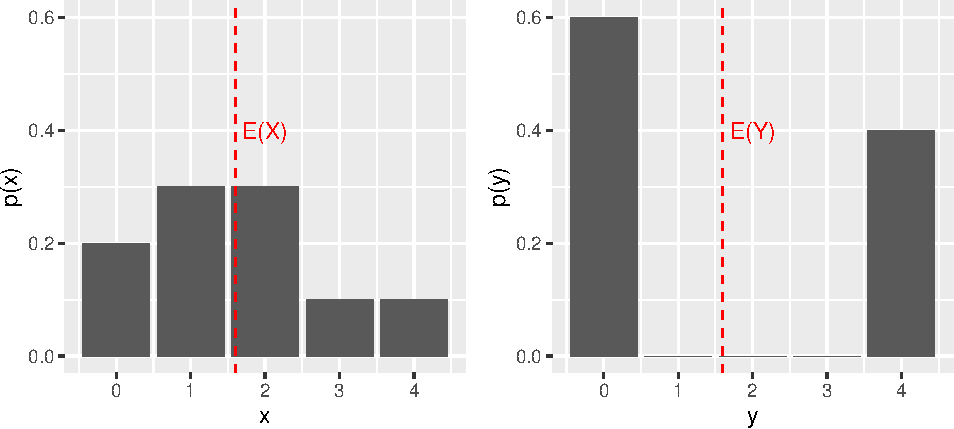
\includegraphics[keepaspectratio]{math340-notes_files/figure-latex/unnamed-chunk-12-1.pdf}}

Observe that this function \(F(x)\) is defined for all \(-\infty < x < \infty\) (check out those arrows :)). The jumps in the graph indicate that the function \(F\) is not continuous, and the points of discontinuity occur exactly at the values of \(X\) in the probability table for \(X\).
\end{example}

\begin{theorem}[Properties of any distribution function]
\protect\hypertarget{thm:dist-fcn-props}{}\label{thm:dist-fcn-props}

If \(F(x)\) is a distribution function, then

\begin{enumerate}
\def\labelenumi{\alph{enumi})}
\tightlist
\item
  \(\displaystyle \lim_{x \to -\infty} F(x) = 0\);
\item
  \(F\) is non-decreasing. That is, if \(x_1 \leq x_2\) then \(F(x_1) \leq F(x_2)\); and
\item
  \(\displaystyle \lim_{x \to \infty} F(x) = 1\).
\end{enumerate}

\end{theorem}

\begin{definition}[Continuous Random Variable]
\protect\hypertarget{def:continuous-rv}{}\label{def:continuous-rv}A random variable is called a \textbf{continuous random variable}\index{random variable!continuous} if its distribution function \(F\) is continuous for all \(x\).
\end{definition}

So the distribution function for any continuous random variable has the following sort of look, descriptively (as in Figure \ref{fig:cont-F}):

\begin{itemize}
\tightlist
\item
  it is continuous,
\item
  its domain is \((-\infty,\infty)\)
\item
  as \(x\) progresses away from \(-\infty\) toward \(\infty,\) the values of \(F(x)\) rise from 0 to 1, never decreasing along the way.
\end{itemize}

\begin{definition}
\protect\hypertarget{def:pdf-continuous-RV}{}\label{def:pdf-continuous-RV}Let \(F\) be the distribution for a continuous random variable \(X\). Then the derivative of \(F,\) wherever it exists is called the \textbf{probability density function}\index{probability density function!continuous random variable} for \(X\). When continuous \(X\) has a probability density function, we usually denote it as \(f(x)\).
\end{definition}

The density function \(f(x)\) is a theoretical curve for the frequency distribution of a population of measurements. We'll look at examples shortly.

\begin{theorem}[Properties of a density function]
\protect\hypertarget{thm:pdf-props}{}\label{thm:pdf-props}

If \(f(x)\) is a density function for a continuous random variable \(X,\) then

\begin{enumerate}
\def\labelenumi{\alph{enumi})}
\tightlist
\item
  \(f(x) \geq 0\) for all \(x,\) and
\item
  \(\displaystyle \int_{-\infty}^{\infty} f(x)~dx = 1\).
\end{enumerate}

\end{theorem}

\emph{Sketch of Proof}:

For a) Recall \(f(x) = F^\prime(x)\). One feature of any distribution function is that it is never decreasing, so its slope (derivative) is never negative. Since \(f(x)\) gives the slope of \(F,\) \(f(x) \geq 0\).

For b) \(F\) is the antiderivative of \(f,\) which is useful to know when we integrate \(f\). Also, \(\displaystyle \int_{-\infty}^{\infty} f(x)~dx\) is an improper integral, which we can tackle by splitting it into two integrals, assuming each of these new integrals converges:

\begin{align*}
\int_{-\infty}^{\infty} f(x)~dx &= \int_{-\infty}^{0} f(x)~dx + \int_{0}^{\infty} f(x)~dx  \\
&= \lim_{a \to -\infty} \int_a^0 f(x)~dx + \lim_{b \to \infty} \int_0^b f(x)~dx \\
&=  \lim_{a \to -\infty} \left[F(0)-F(a)\right] + \lim_{b \to \infty} \left[F(b)-F(0)\right] \\
&= (F(0)-0) + (1 - F(0))  & \text{ by limit properties of } F \\
&= 1.
\end{align*}

\begin{example}
Consider distribution function \(F\) pictured below, where \(c > 0\) is a fixed constant.

\begin{figure}
\centering
\pandocbounded{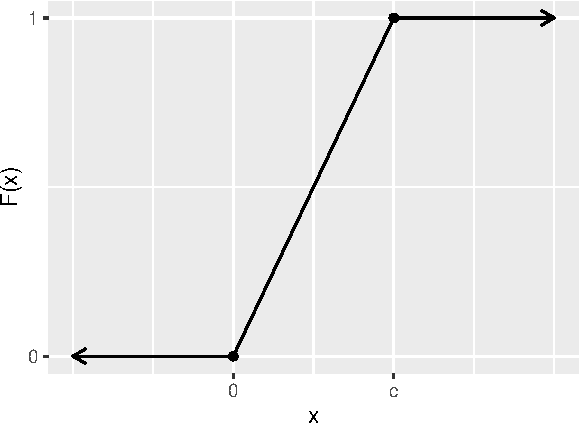
\includegraphics[keepaspectratio]{math340-notes_files/figure-latex/cont-F-1.pdf}}
\caption{\label{fig:cont-F}Piece-wise linear distribution function}
\end{figure}

This function is piece-wise linear, continuous, and it is differentiable everywhere except the sharp corners at \(x = 0\) and \(x = c\). At any other point, \(f(x) = F^\prime(x)\) equals the slope of the segment running through the point \((x,F(X))\).

So the probability density function for this random variable is
\[
f(x)=
\begin{cases}
0 &\text{ if }x < 0 \\
1/c  &\text{ if } 0 < x < c \\
0 &\text{ if } x > c,
\end{cases}
\]
and the graph of \(f\) looks like this:

\begin{figure}
\centering
\pandocbounded{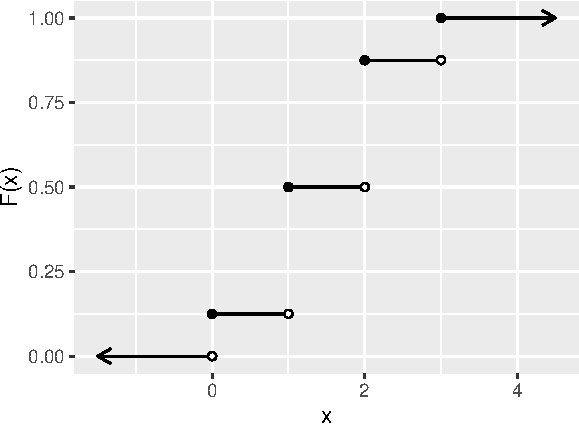
\includegraphics[keepaspectratio]{math340-notes_files/figure-latex/unnamed-chunk-13-1.pdf}}
\caption{\label{fig:unnamed-chunk-13}probability density function for X}
\end{figure}

Note that \(f(x) \geq 0\) for all \(x\). Also, \[\int_{-\infty}^{\infty} f(x)~dx = \int_0^c f(x)~dx\] (we only have to integrate over intervals in which \(f(x) > 0\)), and this later integral is the area of a rectangle of width \(c\) and height \(1/c,\) so it has area 1. Thus, we have a valid pdf!
\end{example}

\begin{example}
Find the value of \(k\) that makes the following function a valid pdf.
\[
f(x)=
\begin{cases}
kx^8 &\text{ if }0 \leq x \leq 1 \\
0 &\text{ else.}
\end{cases}
\]
We need \(k \geq 0\) os that \(f(x) \geq 0\) for all \(x\). We also need
\[1 = \int_{-\infty}^\infty f(x)~dx = \int_0^1 kx^8~dx = \frac{k}{9}x^9 ~\biggr|_0^1.\]
It follows that \(k = 9\).
\end{example}

\begin{definition}[Quantiles]
\protect\hypertarget{def:quantile}{}\label{def:quantile}Let \(X\) denote a random variable. If \(0 < p < 1,\) the \(p\)th quantile of \(X,\) denoted \(\phi_p,\) is the smallest value such that \(F(\phi_p) \geq p\). If \(X\) is continuous, \(\phi_p\) is the smallest value such that \(F(\phi_p) = p\).
\end{definition}

Some special quantiles:

\begin{itemize}
\tightlist
\item
  \(\phi_.25,\) denoted \(Q1,\) is called the first quartile,
\item
  \(\phi_.5,\) denoted \(M,\) is called the median of the random variable,
\item
  \(\phi_.75,\) denoted \(Q3,\) is called the third quartile
\end{itemize}

\begin{theorem}
If \(X\) is a continuous random variable with density function \(f,\) then for any real numbers \(a < b,\)
\[P(a \leq X \leq b) = \int_a^b f(x)~dx.\]
\end{theorem}

\textbf{Proof Idea}: The distribution function \(F\) is an antiderivative of the density function \(f,\) so using the Fundamental Theorem of Calculus,

\begin{align*}
\int_a^b f(x)~dx  &= F(b) - F(a) \\
                  &= P(X\leq b) - P(X \leq a) \\
                  &= P(a < X \leq b) &\text{ since } a < b\\
                  &= P(a \leq X \leq b) &\text{ since } P(X = a) = 0
\end{align*}

\textbf{Note}: For any continuous random variable \(X,\) and \(a < b,\)

\[P(a < X < b) = P(a \leq X < b) = P(a < X \leq b) = P(a \leq X \leq B)\] since \(P(X = c) = 0\) for any real number \(c\).

\begin{example}[A quadratic density function]
\protect\hypertarget{exm:cont-quad-rv}{}\label{exm:cont-quad-rv}

Suppose \(X\) has density function
\[
f(x)=
\begin{cases}
\frac{3}{8}x^2 &\text{ if }0 \leq x \leq 2 \\
0 &\text{ else.}
\end{cases}
\]

Wait! Is this \emph{actually} a valid density function?

\begin{enumerate}
\def\labelenumi{\arabic{enumi}.}
\tightlist
\item
  Ok, yes, \(f(x) \geq 0\) for all \(x\).
\item
  And\ldots{}
\end{enumerate}

\begin{align*}
\int_{-\infty}^{\infty} f(x) ~dx &= \int_0^2 \frac{3}{8} x^2~dx \\
                            &= \frac{1}{8} x^3 \Big|_0^2 \\
                            &= 1.
\end{align*}

Ok, now to the question: Find \(P(1 \leq X \leq 2)\):

\begin{align*}
 P(1 \leq X \leq 2)   &= \int_1^2 \frac{3}{8} x^2~dx \\
                      &= \frac{1}{8} x^3 ~\biggr|_1^2 \\
                      &= 1 - \frac{1}{8} \\
                      &= \frac{7}{8}.
\end{align*}

Even though \(X\) can take any value between 0 and 2, the probability is 7/8 that \(X\) will be between 1 and 2. Most of the area under the density curve is at the high end of the \(X\) range:

\begin{figure}
\centering
\pandocbounded{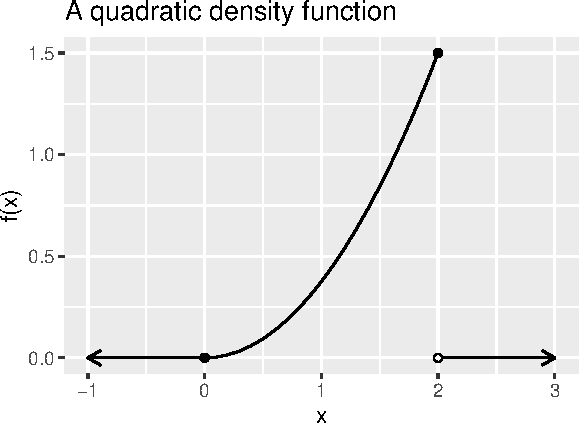
\includegraphics[keepaspectratio]{math340-notes_files/figure-latex/quadratic-density-1.pdf}}
\caption{\label{fig:quadratic-density}A quadratic density function}
\end{figure}

\end{example}

\begin{example}
Suppose \(X\) has density function
\[
f(x)=
\begin{cases}
0 &\text{ if } x < 1 \\
\frac{1}{x^2} &\text{ if } x \geq 1.
\end{cases}
\]

\begin{quote}
\textbf{a)} Check that this gives a valid density function:
\end{quote}

\begin{align*}
 \int_{-\infty}^{\infty} f(x)~dx    &= \int_1^\infty x^{-2}~dx \\
                                    &= \lim_{b \to \infty} \left[\int_1^b x^{-2}~dx \right] \\
                                    &= \lim_{b \to \infty} \left[ -\frac{1}{x} \biggr|_1^b \right]\\
                                    &= \lim_{b \to \infty} \left[ -\frac{1}{b}+1\right]\\
                                    &= 1.
\end{align*}
The limit equals 1 in the end since \(1/b \to 0\) as \(b \to \infty\).

\begin{quote}
\textbf{b)} Find \(F(x),\) the cumulative probability distribution function.
\end{quote}

By definition, for any real number \(x,\) \[F(x) = \int_{-\infty}^x f(t)~dt,\] which, of course, gives the area under \(f\) over the interval \((-\infty, x]\). Since \(f\) is piece-wise defined, the integrand used in the integral to evaluate \(F\) depends on the bounds of the integral.

\[
F(x)=
\begin{cases}
\displaystyle\int_{-\infty}^x 0 ~dt &\text{ if } x < 1 \\
\displaystyle\int_{-\infty}^1 0 ~dt  + \displaystyle\int_{1}^x \frac{1}{t^2} ~dt&\text{ if } x \geq 1.
\end{cases}
\]
We leave it to the reader to integrate these expressions to obtain
\[
F(x)=
\begin{cases}
0 &\text{ if } x < 1 \\
\displaystyle 1 - \frac{1}{x} &\text{ if } x \geq 1.
\end{cases}
\]

\begin{figure}
\centering
\pandocbounded{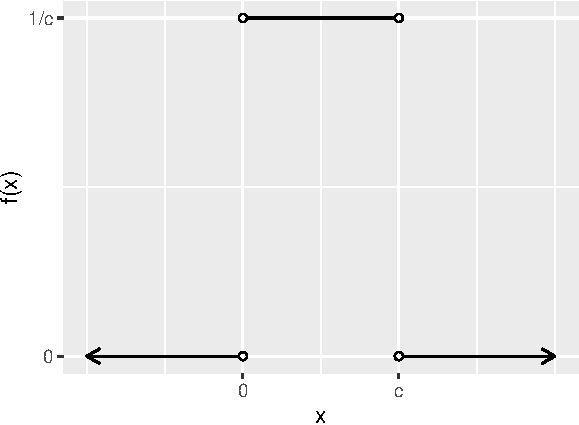
\includegraphics[keepaspectratio]{math340-notes_files/figure-latex/unnamed-chunk-14-1.pdf}}
\caption{\label{fig:unnamed-chunk-14}Distribution function for X}
\end{figure}

\begin{quote}
\textbf{c)} Find \(P(1 < X < 3).\)
\end{quote}

Well, \[P(1 < X < 3) = \int_1^3 f(x)~dx = F(3)-F(1),\] by the Fundamental Theorem of Calculus (FTC), so \[P(1 < X < 3) = (1 - 1/3) - (1 - 1/1) = 2/3.\]
\end{example}

\section{Expected Value for Continuous Random Variables}\label{expected-value-for-continuous-random-variables}

\begin{definition}
\protect\hypertarget{def:expected-value-continuous}{}\label{def:expected-value-continuous}If \(X\) is a continuous random variable with probability density function \(f(x),\) then the \textbf{expected value of \(X\)}\index{expected value!continuous random variable}, denoted \(E(X),\) is \[E(X) = \int_{-\infty}^\infty x \cdot f(x)~dx,\] provided this integral exists. The expected value \(E(X)\) is also called the \textbf{mean of \(X\)}\index{mean of a random variable}, and is often denoted as \(\mu_X,\) or \(\mu\) if the random variable \(X\) is understood.

The \textbf{expected value of the function \(g(X)\) of \(X\)} is \[E(g(X)) = \int_{-\infty}^\infty g(x) \cdot f(x)~dx,\] provided this integral exists.

The \textbf{variance of \(X\)} is \[V(X) = E((X-\mu_X)^2),\] provided this integral exists.
\end{definition}

As in the discrete case, one can show \(V(X) = E(X^2)-E(X)^2,\) a working formula for variance which is sometimes easier to use to calculate variance.

\begin{example}
\leavevmode

\begin{quote}
Find \(E(X)\) and \(V(X)\) where \(X\) is the continuous random variable from Example \ref{exm:cont-quad-rv}.
\end{quote}

Recall \(X\) has density function \(\displaystyle f(x) = 3x^2/8\) for \(0 \leq x \leq 2\).

Expected Value:
\begin{align*}
E(X) &= \int_0^2 x \cdot 3x^2/8~dx \\
      &= \frac{3}{8} \int_0^2 x^3~dx \\
      &= \frac{3}{8}\frac{1}{4}x^4 ~\biggr|_0^2 \\
      &= \frac{3}{2}.
\end{align*}

Variance:
We first find \(E(X^2)\):
\begin{align*}
E(X^2) &= \int_0^2 x^2 \cdot 3x^2/8~dx \\
      &= \frac{3}{8} \int_0^2 x^4~dx \\
      &= \frac{3}{8}\frac{1}{5}x^5 ~\biggr|_0^2 \\
      &= \frac{12}{5}.
\end{align*}

Then,
\begin{align*}
V(X)    &= E(X^2) - E(X)^2 \\
        &= (12/5) - (3/2)^2\\
        &= 0.15.
\end{align*}

The properties of expected value that held for discrete random variables also hold for continuous random variables.

\end{example}

\begin{theorem}
\protect\hypertarget{thm:EV-properties-continuous}{}\label{thm:EV-properties-continuous}

Suppose \(X\) is a continuous random variable, \(c \in \mathbb{R}\) is a constant, and \(g,\) \(g_1,\) and \(g_2\) are functions of \(X\).

\begin{enumerate}
\def\labelenumi{\arabic{enumi}.}
\tightlist
\item
  \(E(c) = c\).
\item
  \(E(c\cdot g(X))= cE(g(X))\).
\item
  \(E(g_1(X) \pm g_2(X)) = E(g_1(X)\pm g_2(X))\).
\end{enumerate}

\end{theorem}

These results follow immediately from properties of integration. For instance, to prove property 1 we observe
that for constant \(c,\)
\[E(c) = \int_{-\infty}^\infty c\cdot f(x)~ dx  = c \int_{-\infty}^\infty f(x)~ dx,\]
and the integral in the last expression equals 1 by definition of a valid probability density function.

\begin{theorem}
\protect\hypertarget{thm:EV-linear-props}{}\label{thm:EV-linear-props}

Let \(X\) be a random variable (discrete or continuous) with \(E(X) = \mu\) and \(V(X) = \sigma^2,\) and let \(a, b\) be constants. Then

\begin{enumerate}
\def\labelenumi{\alph{enumi})}
\tightlist
\item
  \(\displaystyle E(aX + b) = aE(X) + b = a \mu + b.\)
\item
  \(\displaystyle V(aX + b) = a^2V(X) = a^2 \sigma^2.\)
\end{enumerate}

\end{theorem}

\begin{proof}
\leavevmode

\begin{enumerate}
\def\labelenumi{\alph{enumi})}
\item
  This result follows immediately from properties of expected value (Theorems \ref{thm:EV-properties-continuous} and \ref{thm:EV-properties-continuous}).
\item
  Let \(Y = aX + b\). Then (a) says that \(E(Y) = a \mu + b,\) so
  \begin{align*}
  V(Y) &= E((Y-(a\mu + b))^2) \\
   &= E\left(((aX+b)-(a\mu + b))^2\right)\\
   &= E\left((aX-a\mu)^2\right)\\
   &= a^2 E\left((X-\mu)^2\right)
  \end{align*}
  But \(E\left((X-\mu)^2\right)=V(X)\) by the definition of variance, so the result follows.
\end{enumerate}

\end{proof}

\begin{example}[Ore Sample Impurities]
\protect\hypertarget{exm:ore-samples}{}\label{exm:ore-samples}For certain ore samples, the proportion \(X\) of impurities per sample is a random variable with density function
\[
f(x)=
\begin{cases}
1.5x^2 + x &\text{ if }0 \leq x \leq 1 \\
0 &\text{ else. }
\end{cases}
\]
The dollar value of each sample is \(W = 5 - 0.5X\).

\begin{quote}
Find the mean, variance, and standard deviation of \(W\).
\end{quote}

First, let's consider the variable \(X\) itself.

\begin{align*}
E(X) &= \int_0^1 x \cdot (1.5x^2 + x)~dx \\
      &= \int_0^1 1.5x^3 + x^2~dx \\
      &= \frac{1.5}{4}x^4 + \frac{1}{3} x^3 ~\biggr|_0^1 \\
      &= \frac{17}{24}.
\end{align*}

Also,
\begin{align*}
E(X^2) &= \int_0^1 x^2 \cdot (1.5x^2 + x)~dx \\
      &= \int_0^1 1.5x^4 + x^3~dx \\
      &= \frac{1.5}{5}x^5 + \frac{1}{4} x^4 ~\biggr|_0^1 \\
      &= \frac{11}{20}.
\end{align*}

Thus, \(V(X) = (11/20)-(17/24)^2 \approx 0.0483.\)

Then, by Theorem \ref{thm:EV-linear-props},

\[E(W) = E(5 - 0.5X) = 5 - 0.5E(X) = 5 - 0.5\cdot (17/24) = 4.65,\]
and
\[V(W) = V(5 - 0.5X) = 0.25V(X) \approx 0.012,\]
so that the standard deviation is \(\sigma = \sqrt{V(W)} ~\approx 0.11\) (about 11 cents).
\end{example}

:::

\chapter{Important Continuous Random Variables}\label{important-continuous-rv}

In this chapter we introduce the following well-known continuous random variables:
uniform, normal, exponential, gamma, chi-square, and beta. In examples we work through, it will from time to time be convenient to compute probabilities in R. Appendix \ref{R-continuousRV} contains details about the commands in R useful for doing so.

\section{Uniform Distribution}\label{uniform-continuous}

\begin{definition}
\protect\hypertarget{def:uniform-distribution}{}\label{def:uniform-distribution}Let \(\theta_1 < \theta_2\) be distinct real numbers. A random variable \(X\) has \textbf{uniform distribution on the interval \([\theta_1,\theta_2]\)}\index{uniform distribution} if it has probability density function
\[
f(x)=
\begin{cases}
\frac{1}{\theta_2 - \theta_1} &\text{ if }\theta_1 \leq x \leq \theta_2 \\
0 &\text{ else.} 
\end{cases}
\]
we may write \(X ~\sim~ U(\theta_1,\theta_2)\)\index{U$(\theta_1,\theta_2)$} to mean \(X\) is uniform on \([\theta_1,\theta_2]\).
\end{definition}

A uniform random variable is a good model for picking a random real number between \(\theta_1\) and \(\theta_2\).

In R we access the uniform distribution with \texttt{unif}. For instance, we can generate a random sample of \(n\) numbers in the interval \([a,b]\) with the \texttt{runif()} command:

\begin{Shaded}
\begin{Highlighting}[]
\NormalTok{n}\OtherTok{=}\DecValTok{6}\NormalTok{; a }\OtherTok{=} \DecValTok{0}\NormalTok{; b }\OtherTok{=} \DecValTok{10}\NormalTok{;}
\FunctionTok{runif}\NormalTok{(n,a,b)}
\end{Highlighting}
\end{Shaded}

\begin{verbatim}
## [1] 9.366265 4.699564 6.208853 6.012264 5.983060 6.560475
\end{verbatim}

\begin{example}[Average value of a function]
\leavevmode

\begin{quote}
Use R to estimate the average value of \(f(x) = x^2\) over the interval {[}0,2{]}.
\end{quote}

Our strategy: Select a large random sample of points in the interval {[}0,2{]} and then compute the average of their squares.

\begin{Shaded}
\begin{Highlighting}[]
\NormalTok{x }\OtherTok{=} \FunctionTok{runif}\NormalTok{(}\DecValTok{1000}\NormalTok{,}\DecValTok{0}\NormalTok{,}\DecValTok{2}\NormalTok{) }\CommentTok{\#picking 1000 points in [0,2]}
\FunctionTok{mean}\NormalTok{(x}\SpecialCharTok{\^{}}\DecValTok{2}\NormalTok{)}
\end{Highlighting}
\end{Shaded}

\begin{verbatim}
## [1] 1.295235
\end{verbatim}

\textbf{Note}: From Calc I, we know the average value of a function \(f\) over the interval \([a,b]\) is \[\frac{1}{b-a} \int_a^b f(x)~dx,\]
so here it's \[\frac{1}{2}\int_0^2 x^2~dx = \frac{1}{6} x^3 ~\biggr|_0^2 = 4/3 \approx 1.333.\]

\end{example}

\begin{theorem}
\protect\hypertarget{thm:uniform-EandV}{}\label{thm:uniform-EandV}If \(X\) is \(U(\theta_1,\theta_2),\) then \[E(X) = \frac{\theta_1 + \theta_2}{2}, ~~~ \text{ and } ~~~ V(X) = \frac{(\theta_2-\theta_1)^2}{12}.\]
\end{theorem}

\begin{proof}
Recall, \(X\) has pdf
\[
f(x)=
\begin{cases}
\frac{1}{\theta_2 - \theta_1} &\text{ if }\theta_1 \leq x \leq \theta_2 \\
0 &\text{ else.} 
\end{cases}
\]
So

\begin{align*}
E(X) &= \int_{\theta_1}^{\theta_2} x \cdot \frac{1}{\theta_2-\theta_1}~dx\\
      &= \frac{1}{\theta_2-\theta_1} \cdot \frac{1}{2}x^2 ~\biggr|_{\theta_1}^{\theta_2}\\
      &= \frac{1}{\theta_2-\theta_1} \cdot \frac{1}{2}(\theta_2^2-\theta_1^2) \\
      &= \frac{1}{\theta_2-\theta_1} \cdot \frac{1}{2}(\theta_2-\theta_1)(\theta_2+\theta_1) \\
      &= \frac{\theta_1+\theta_2}{2}.
\end{align*}

One can show similarly, that \[E(X^2) = \int_{\theta_1}^{\theta_2} x^2 \cdot \frac{1}{\theta_2-\theta_1}~dx = \cdots =  \frac{\theta_2^2 + \theta_1\theta_2 + \theta_1^2}{3},\]
so that \[V(X) = E(X^2) - E(X)^2 = \frac{(\theta_2-\theta_1)^2}{12}.\] The fun algebra details are left to the reader.
\end{proof}

\section{Exponential Distribution}\label{exponential-distribution}

The exponential distribution is often used to model experiments that aim to investigate: How long until something happens?

\begin{definition}
\protect\hypertarget{def:exp-distribution}{}\label{def:exp-distribution}A random variable \(X\) has an \textbf{exponential probability distribution with parameter \(\beta\)}\index{exponential distribution}, denoted \(\texttt{Exp}(\beta)\)\index{\texttt{Exp}$(\beta)$}, if it has probability density function
\[
f(x)=
\frac{1}{\beta}e^{-(x/\beta)} ~~~ \text{ for }x \geq 0~~~ \text{ (and }f(x) = 0\text{ else.)}
\]
\end{definition}

First, let's check that the total area under \(f(x)\) is 1.

\begin{align*}
\int_0^\infty \frac{1}{\beta}e^{-x/\beta}~dx &= \lim_{b\to\infty}\left[\int_0^b \frac{1}{\beta}e^{-x/\beta}~dx\right] \\
&= \lim_{b\to\infty}\left[-e^{-x/\beta}\biggr|_0^b \right] & \text{(try u-sub.} u=-x/\beta) \\
&= \lim_{b \to \infty}\left[1 - \frac{1}{e^{b/\beta}}\right]\\
&= 1.
\end{align*}

Having done the above integral, we can write down a formula for the cumulative distribution function for an exponential distribution:

If \(X\) is \(\texttt{Exp}(\beta)\) then for \(x \geq 0,\)
\begin{align*}
F(x) &= \int_0^x \frac{1}{\beta}e^{-t/\beta}~dt\\
    &= 1 - e^{-x/\beta}.
\end{align*}

\begin{example}
Suppose \(X\) is \(\texttt{Exp}(\beta)\). Find \(P(X < 8)\).

Well,
\begin{align*}
P(X < 8) &= F(8)\\
        &= 1 - e^{-8/4} \\
        &= 1 - e^{-2} \\
        &\approx .865.
\end{align*}
\end{example}

\begin{theorem}
\protect\hypertarget{thm:exponential-EandV}{}\label{thm:exponential-EandV}If \(X\) is \(\texttt{Exp}(\beta),\) then \[E(X) = \beta, ~~~ \text{ and } ~~~ V(X) = \beta^2.\]
\end{theorem}

\begin{proof}
\begin{align*}
E(X)&= \int_0^\infty x\cdot\frac{1}{\beta} e^{-x/\beta}~dx \\
    &= \lim_{b \to \infty}\left[\int_0^b x\cdot\frac{1}{\beta} e^{-x/\beta}~dx\right]
\end{align*}

To evaluate this integral, try integration by parts with \(u = x\) and \(dv = e^{-x/\beta}~dx\). Doing so, we obtain
\begin{align*}
E(X) &= \lim_{b \to \infty}\left[\int_0^b x\cdot\frac{1}{\beta} e^{-x/\beta}~dx\right]\\
    &= \lim_{b \to \infty}\left[-xe^{-x/\beta} - \beta e^{-x/\beta}\biggr|_0^b\right]\\
    &= \lim_{b \to \infty}\left[\left(\frac{-b}{e^{b/\beta}} - \frac{\beta}{e^{b/\beta}}\right) - \left(0 - \beta\right)\right].
\end{align*}
Since \(\displaystyle \frac{b}{e^{b/\beta}} \to 0\) and \(\displaystyle \frac{\beta}{e^{b/\beta}} \to 0\) as \(b \to \infty,\) we have proved that \(E(X) = \beta.\)

To prove that \(V(X) = \beta^2,\) first find \(E(X^2)=\int_0^\infty x^2 f(x)~dx\) by integration by parts, and then use the fact that \(V(X) = E(X^2)-E(X)^2\). We leave details to those nostalgic for Calc II. :)
\end{proof}

\section{Normal Distribution}\label{normal}

\begin{definition}
\protect\hypertarget{def:normal-distribution}{}\label{def:normal-distribution}A random variable \(X\) has a \textbf{normal probability distribution with parameters \(\mu\) and \(\sigma > 0\)}\index{normal distribution}, denoted \(N(\mu,\sigma)\)\index{N$(\mu,\sigma)$}, if it has probability density function
\[
f(x)=\frac{1}{\sigma\sqrt{2\pi}}e^{-\frac{(x-\mu)^2}{2\sigma^2}}, \text{ for } -\infty < x < \infty.
\]
\end{definition}

The graph of a normal density curve is bell-shaped, with peak at \(x = \mu,\) and inflection points at \(x = \mu \pm \sigma,\) facts we can readily demonstrate by analyzing the first and second derivative of \(f\).

\begin{figure}
\centering
\pandocbounded{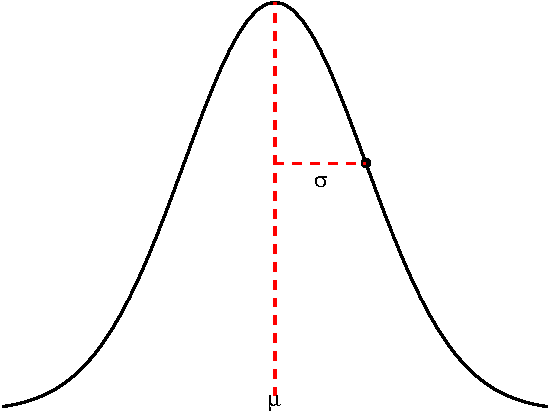
\includegraphics[keepaspectratio]{math340-notes_files/figure-latex/bell-curve-1.pdf}}
\caption{\label{fig:bell-curve}A Normal density curve}
\end{figure}

\begin{theorem}
\protect\hypertarget{thm:normal-EandV}{}\label{thm:normal-EandV}If \(X\) is \(N(\mu,\sigma),\) then \[E(X) = \mu, ~~~ \text{ and } ~~~ V(X) = \sigma^2.\]
\end{theorem}

\begin{definition}
\protect\hypertarget{def:standard-normal}{}\label{def:standard-normal}The \textbf{standard normal probability distribution} is \(N(0,1)\). If \(Z\) is \(N(0,1),\) its pdf is \[f(z) = \frac{1}{\sqrt{2\pi}}e^{-z^2/2}, \text{ for all real numbers } z.\]
\end{definition}

As we shall see, the family of normal distributions \(N(\mu,\sigma)\) has a special place of importance in statistics; many distributions have a bell-shape (physical measurements, for instance, such as heights of adult males, weights of newborns, wingspans of adult female bald eagles, \ldots). But its special place of importance in statistics comes from the fact that the distribution of sample means from repeated sampling, as we shall see, are well-modeled by normal distributions.

\begin{theorem}
\protect\hypertarget{thm:standardizing-normal-distributions}{}\label{thm:standardizing-normal-distributions}If \(X\) is \(N(\mu,\sigma)\) then \(Z = (X-\mu)/\sigma\) is \(N(0,1)\).
\end{theorem}

We prove this theorem later.

In practice, shifting from \(X\) to \[Z = \frac{X-\mu}{\sigma}\] gives us a way to consider unitless, standardized ``Z-scores'' associated to values in \(X\).

A Z-score for \(X\) gives the number of standard deviations above or below the mean \(X\) is in its distribution.

\begin{example}[The 68-95-99.7 Rule]
\protect\hypertarget{exm:normal-rule-of-thumb}{}\label{exm:normal-rule-of-thumb}

In any normal distribution \(N(\mu, \sigma)\):

\begin{itemize}
\tightlist
\item
  About 68\% of the distribution is within 1 standard deviation of the mean.
\item
  About 95\% of the distribution is within 2 standard deviations of the mean.
\item
  About 99.7\% of the distribution is within 2 standard deviations of the mean.
\end{itemize}

\pandocbounded{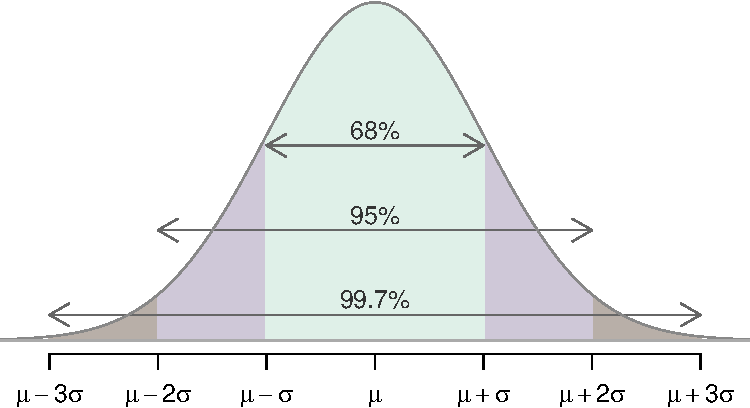
\includegraphics[keepaspectratio]{math340-notes_files/figure-latex/unnamed-chunk-17-1.pdf}}

For instance, in \(N(10,3),\)

\begin{itemize}
\tightlist
\item
  Roughly, 68\% of the distribution is between 7 and 13, and
\item
  95\% of the distribution is between 4 and 16, and
\item
  99.7\% of the distribution is between 1 and 19.
\end{itemize}

\end{example}

\begin{example}
\protect\hypertarget{exm:comparing-values-with-z-scores}{}\label{exm:comparing-values-with-z-scores}Which is more ``impressive'': hitting 50 home runs in a season when the league home run distribution is \(N(35,9),\) or hitting 35 home runs in a season when the league distribution is \(N(24,5)\)?

For 50 in \(N(35,9),\) \[Z = \frac{50-35}{9} = \frac{5}{3} \approx 1.67.\]

\pandocbounded{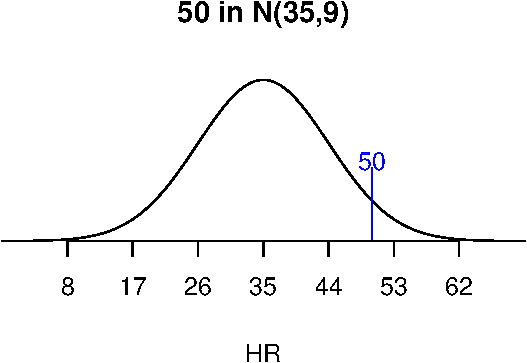
\includegraphics[keepaspectratio]{math340-notes_files/figure-latex/unnamed-chunk-18-1.pdf}}

For 35 in \(N(24,5),\) \[Z = \frac{35-24}{5} = \frac{11}{5} = 2.2.\]

\pandocbounded{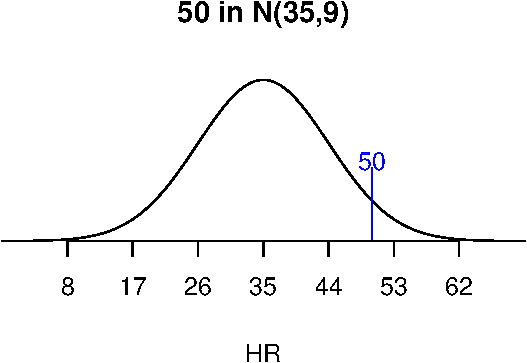
\includegraphics[keepaspectratio]{math340-notes_files/figure-latex/unnamed-chunk-19-1.pdf}}

A person hitting 35 HR in a league with distribution \(N(24,5)\) is more extreme (at the high end), and so more impressive in that sense.
\end{example}

Now we focus on some fine print, proving that the density function for a normal distribution is, indeed, a valid density function.

\begin{lemma}
\[\int_{-\infty}^{\infty} e^{-x^2/2}~dx = \sqrt{2\pi}.\]
\end{lemma}

\begin{proof}
First, we remark that the integral converges by comparison with \(\displaystyle \int_{-\infty}^{\infty} e^{-x/2}~dx.\)

Suppose the value of the integral we want to calculate is \(A\). We use some integration techniques from vector calculus to first find the value of \(A^2\). If you haven't seen vector calculus, don't sweat the details, but demand your vector calculus prof prove this lemma when you take the class :). Ok, let's look at \(A^2\).
\begin{align*}
A^2 &= \left(\int_{-\infty}^{\infty} e^{-x^2/2}~dx \right)\left(\int_{-\infty}^{\infty} e^{-y^2/2}~dy \right)\\
    &= \int_{-\infty}^{\infty} \int_{-\infty}^{\infty} e^{-x^2/2} e^{-y^2/2} dx dy \\
    &= \int_{-\infty}^{\infty} \int_{-\infty}^{\infty} e^\frac{-(x^2+y^2)}{2} ~dx dy \\
    &= \int_0^{2\pi}\int_0^\infty e^{-r^2/2}~r ~dr~ d\theta &\text{ change to polar coordinates}\\
    &= 2\pi \int_0^\infty e^{-r^2/2}~r ~dr \\
    &= -\pi \int_0^\infty e^{-u} ~du & \text{ let } u = r^2/2 \\
    &= 2\pi \left[-e^{-u} \biggr|_0^\infty \right]
    &= 2\pi [-0 + 1] \\
    &= 2\pi
\end{align*}

Since \(A^2 = 2\pi,\) \(A = \sqrt{2\pi}\).
\end{proof}

We have the following corollaries to this lemma.

\begin{corollary}
The function \(f(x) = \frac{1}{\sqrt{2\pi}}e^{-x^2/2},\) for \(-\infty < x < \infty,\) is a valid probability density function.
\end{corollary}

\begin{proof}
Clearly, \(f(x) \geq 0\) for all \(x,\) and the previous lemma ensures that \(\int_{-\infty}^\infty f(x)~dx = 1.\).
\end{proof}

\begin{corollary}
The function \(f(x) = \frac{1}{\sigma\sqrt{2\pi}}e^{-(x-\mu)^2/(2\sigma^2)},\) for \(-\infty < x <  \infty,\) is a valid probability density function.
\end{corollary}

\begin{proof}
Clearly, \(f(x) \geq 0\) for all \(x,\) and after \(u\)-substitution of \(u = (x-\mu)/\sigma,\) the previous lemma ensures that \(\int_{-\infty}^\infty f(x)~dx = 1\).
\end{proof}

\section{Gamma Distribution}\label{gamma-distribution}

Some random variables are always nonnegative and yield distributions of data that are skewed right, as pictured below.

\pandocbounded{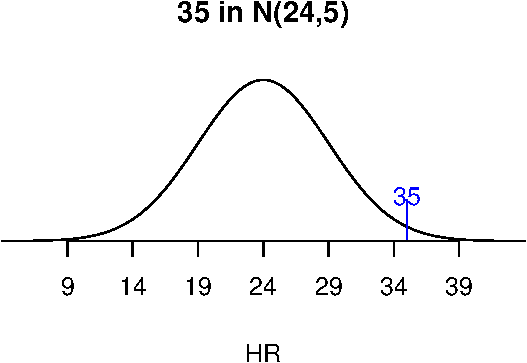
\includegraphics[keepaspectratio]{math340-notes_files/figure-latex/unnamed-chunk-20-1.pdf}}

Some typically skewed right distributions include household incomes in a city, the length of time between malfunctions of some machine, and major league baseball salaries. The gamma probability distribution, which has two parameters \(\alpha\) and \(\beta,\) can model such skewed right distributions. The parameter \(\alpha\) is sometimes called the \textbf{shape} parameter, \(\beta\) is called the \textbf{scale} parameter, and its reciprocal \(1/\beta\) is called the \textbf{rate}.

The density function for a gamma distribution looks formidable, so we'll take time to go through it carefully.

\begin{definition}
\protect\hypertarget{def:gamma-distribution}{}\label{def:gamma-distribution}A random variable \(X\) has a \textbf{gamma probability distribution with parameters \(\alpha>0\) and \(\beta>0\)}\index{gamma distribution}, denoted \(\texttt{gamma}(\alpha,\beta)\)\index{\texttt{gamma}$(\alpha,\beta)$}, if and only if it has probability density function
\[
f(x)=
\frac{1}{\beta^\alpha \Gamma(\alpha)}x^{\alpha-1}e^{-(x/\beta)}~~~ \text{ for }x \geq 0~~~ \text{ (and }f(x) = 0\text{ else)}
\]
where \[\Gamma(\alpha) = \int_0^\infty t^{\alpha-1}e^{-t}~dt\] is called the \textbf{gamma function}\index{gamma function}.
\end{definition}

Here are plots of three different gamma distributions.

\begin{figure}
\centering
\pandocbounded{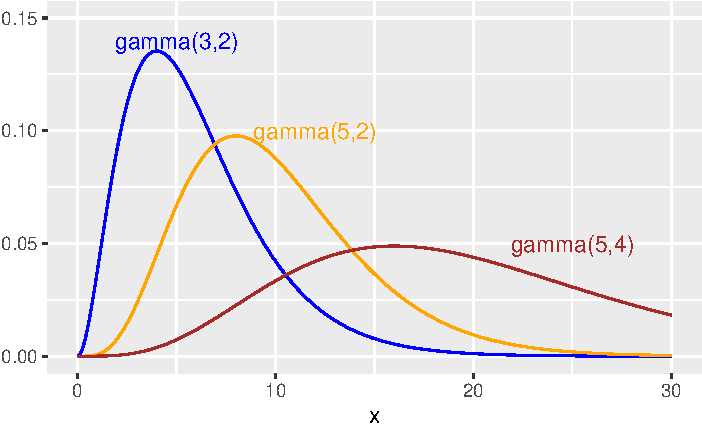
\includegraphics[keepaspectratio]{math340-notes_files/figure-latex/gamma-plots-1.pdf}}
\caption{\label{fig:gamma-plots}Some gamma density functions}
\end{figure}

The quantity \(\Gamma(\alpha)\) is called the \textbf{gamma function}\index{gamma function}, which has some nice features.

\begin{lemma}
\protect\hypertarget{lem:gamma-fcn-ind-step}{}\label{lem:gamma-fcn-ind-step}If \(n > 0\) then \(\Gamma(n+1) = n \cdot \Gamma(n).\)
\end{lemma}

\begin{proof}
This follows by integration by parts!
First note,
\[
\Gamma(n+1) = \int_0^\infty t^{(n+1)-1}e^{-t}~dt = \int_0^\infty t^n e^{-t}~dt.
\]

Let \(u = t^n,\) and \(dv = e^{-t}~dt\). Then \(du = nt^{n-1}~dt\) and \(v = -e^{-t},\) and

\begin{align*}
\int_0^\infty t^n e^{-t}~dt &= -t^ne^{-t}\biggr|_0^\infty - \int_0^\infty nt^{n-1}(-e^{-t})~dt \\
      &= \lim_{b \to \infty}\left[-t^ne^{-t}\biggr|_0^b\right]+n\int_0^\infty t^{n-1}e^{-t}~dt
\end{align*}

Apply l'hopital's rule to see that the limit term above evaluates to 0, and note the integral term above is precisely the definition of \(\Gamma(n)\).
Thus, we have
\[ \Gamma(n+1) = n \cdot \Gamma(n).\]
\end{proof}

This lemma provides us with the following

\begin{quote}
\textbf{Fun Fact}:
\(\Gamma(n) = (n-1)!\) for any positive integer \(n\).
\end{quote}

To see why this is the case, we first show \(\Gamma(1) = 1\):

\begin{align*}
\Gamma(1) &= \int_0^\infty t^0e^{-t}~dt\\
          &= \lim_{b\to\infty}\left[\int_0^b e^{-t}~dt\right]\\
          &= \lim_{b\to\infty}^\infty\left[-e^{-t}\biggr|_0^b\right]\\
          &= \lim_{b\to\infty}^\infty\left[-e^{-b}+1\right]\\
          &= 1.
\end{align*}

Next, the lemma gives us a recursive way to find
\(\Gamma(2), \Gamma(3), \Gamma(4)\) and so on. Or, using mathematical induction, \(\Gamma(1) = 1\) is our basis step, and the inductive step is proved as follows:
Suppose \(\Gamma(k) = (k-1)!\) for some \(k \geq 1\). Then

\begin{align*}
\Gamma(k+1) &= k\cdot \Gamma(k) &\text{ by the lemma }\\
            &= k \cdot (k-1)! &\text{ by substitution}\\
            &= k!
\end{align*}

It follows that \(\Gamma(n) = (n-1)!\) for all positive integers \(n\).

\begin{theorem}
\protect\hypertarget{thm:gamma-EandV}{}\label{thm:gamma-EandV}If \(X\) is \(\texttt{gamma}(\alpha,\beta)),\) then \[E(X) = \alpha\beta, ~~~ \text{ and } ~~~ V(X) = \alpha\beta^2.\]
\end{theorem}

We prove this later in Chapter \ref{mgf}.

\begin{example}

Where does the peak of the \(\texttt{gamma}(\alpha,\beta)\) pdf occur?

This looks like a question for calculus. We can find \(f^\prime,\) set it to 0, and consider critical points.

We leave the details to the reader for now, but find the following results:

\begin{itemize}
\tightlist
\item
  if \(\alpha \leq 1,\) \(f^\prime(x) < 0\) for all \(x > 0,\) so \(f\) is always decreasing and the peak occurs when \(x = 0\).
\item
  If \(\alpha > 1,\) the pdf for \(X \sim \texttt{gamma}(\alpha, \beta)\) has its peak at \(x = (\alpha-1)\beta.\)
\end{itemize}

\end{example}

The family of gamma distributions contain two special sub-families, one of which we've already seen!

\subsection{Exponential Distribution}\label{exponential-distribution-1}

Set \(\alpha = 1\) and you will find \(\texttt{gamma}(1,\beta) = \texttt{Exp}(\beta),\)
because their density functions are identical. So exponential distributions are special gamma distributions.

\subsection{Chi-square distribution}\label{chi-square-distribution}

\begin{definition}
\protect\hypertarget{def:chi-square}{}\label{def:chi-square}Let \(\nu\) be a positive integer. \(X\) has a \textbf{chi-square distribution with \(\nu\) degrees of freedom}\index{chi-square distribution}, denoted \(X\) is \(\chi^2(\nu)\)\index{$\chi^2(\nu)$}, if \(X\) is \(\texttt{gamma}(\alpha = \nu/2, \beta = 2).\)
\end{definition}

Here are plots of three different chi-square distributions.

\begin{center}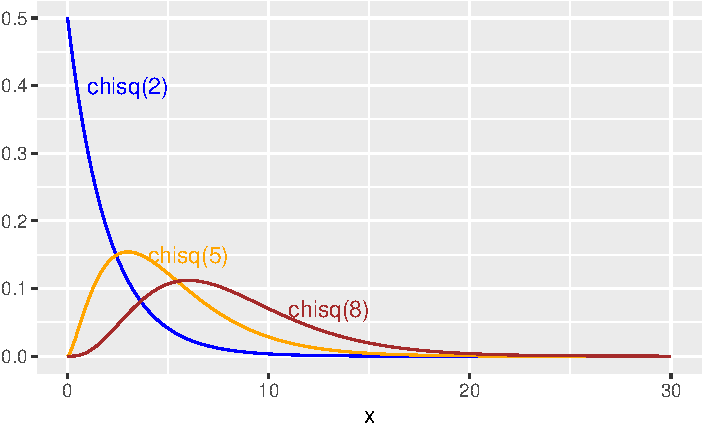
\includegraphics{math340-notes_files/figure-latex/unnamed-chunk-21-1} \end{center}

\section{Beta Distribution}\label{beta-distribution}

The beta probability distribution provides a way to model random variables whose possible outcomes are all real numbers between 0 and 1. Such distributions are useful for modeling proportions. As with the gamma and normal distributions, this is a 2-parameter family of distributions. Altering the parameters \(\alpha\) and \(\beta\) gives us, well, different shapes for the density curves.

\begin{definition}
\protect\hypertarget{def:beta-distribution}{}\label{def:beta-distribution}A random variable \(X\) has a \textbf{beta probability distribution with parameters \(\alpha>0\) and \(\beta>0\)}\index{beta distribution} if and only if it has probability density function
\[
f(x)=
\frac{\Gamma(\alpha + \beta)}{\Gamma(\alpha)\cdot \Gamma(\beta)}x^{\alpha-1}(1-x)^{\beta-1}~~~ \text{ for }0 \leq x \leq 1~~~ \text{ (and }f(x) = 0\text{ else)}
\]

If \(X\) has such a pdf we say that \(X\) is \(\texttt{beta}(\alpha,\beta)\)\index{\texttt{beta}$(\alpha,\beta)$}.
\end{definition}

The gamma function (\ref{def:gamma-distribution}) appears in this pdf three times. Recall that for positive integers \(n,\) \(\Gamma(n) = (n-1)!\) so for integer values of \(\alpha\) and \(\beta,\) the beta density function is fairly nice.
Indeed,

\begin{itemize}
\tightlist
\item
  \(\displaystyle X \sim \texttt{beta}(1,1) \Rightarrow f(x) = \frac{\Gamma(2)}{\Gamma(1)\Gamma(1)}x^0(1-x)^0 = 1\). Whoa! \(\text{beta}(1,1)\) is the uniform distribution \(U(0,1).\)
\item
  \(\displaystyle X \sim \texttt{beta}(1,2) \Rightarrow f(x) = 2(1-x)\).
\item
  \(\displaystyle X \sim \texttt{beta}(2,1) \Rightarrow f(x) = 2x\).
\item
  \(\displaystyle X \sim \texttt{beta}(2,2) \Rightarrow f(x) = 6x(1-x)\).
\item
  \(\displaystyle X \sim \texttt{beta}(n,1) \Rightarrow f(x) = nx^{n-1}\).
\item
  \(\displaystyle X \sim \texttt{beta}(1,n) \Rightarrow f(x) = n(1-x)^{n-1}\).
\end{itemize}

Here are a few beta distributions:
\pandocbounded{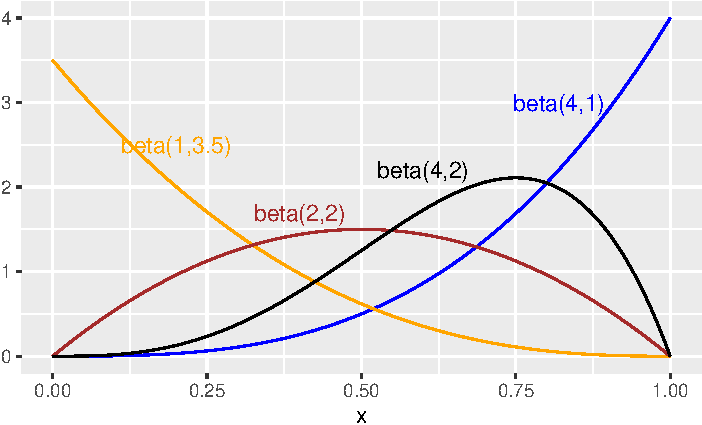
\includegraphics[keepaspectratio]{math340-notes_files/figure-latex/unnamed-chunk-22-1.pdf}}

\begin{theorem}
\protect\hypertarget{thm:beta-EandV}{}\label{thm:beta-EandV}If \(X\) is \(\texttt{beta}(\alpha,\beta)),\) then \[E(X) = \frac{\alpha}{\alpha+\beta}, ~~~ \text{ and } ~~~ V(X) = \frac{\alpha\beta}{(\alpha+\beta)^2(\alpha+\beta+1)}.\]
\end{theorem}

\chapter{Moment Generating Functions}\label{mgf}

Recall by Definition \ref{def:moment-generating-function}, the moment-generating function (mgf) associated with a discrete random variable \(X,\) should it exist, is given by \[m_X(t) = E(e^{tX})\] where the function is defined on some open interval of \(t\) values containing 0. The same definition applies to continuous random variables. We have seen that this mgf encodes information about \(X\): the \(k\)th derivative of \(m\) evaluated at \(t = 0\) gives us the \(k\)th moment. That is, for \(k = 1,2,3,\ldots,\)
\[m_X^{(k)}(0) = E(X^k).\]
In fact, it turns out that the mgf gives us \emph{all} the information about a random variable \(X,\) per the following theorem, whose proof is beyond the scope of this course.

\begin{theorem}
\protect\hypertarget{thm:unique-mgf}{}\label{thm:unique-mgf}Let \(m_X(t)\) and \(m_Y(t)\) denote the mgfs of random variables \(X\) and \(Y,\) respectively. If both mgfs exist and \(m_X(t) = m_Y(t)\) for all values of \(t\) then \(X\) and \(Y\) have the same probability distribution.
\end{theorem}

\begin{example}
\leavevmode

\begin{quote}
Find the mgf for the standard normal random variable \(Z \sim N(0,1)\).
\end{quote}

\begin{align*}
m_Z(t) &= E(e^{tZ})\\
      &= \int_{-\infty}^\infty \frac{1}{\sqrt{2\pi}}e^{-z^2/2}\cdot e^{tz}~dz\\
      &= \frac{1}{\sqrt{2\pi}} \int_{-\infty}^\infty e^{tz-z^2/2}~dz\\
      &= \frac{1}{\sqrt{2\pi}} \int_{-\infty}^\infty e^{-\frac{1}{2}(z-t)^2+\frac{1}{2}t^2}~dz &\text{complete the square}\\
      &= e^{\frac{1}{2}t^2}\left[\frac{1}{\sqrt{2\pi}} \int_{-\infty}^\infty e^{-\frac{1}{2}(z-t)^2}~dz\right]
\end{align*}

The bracketed portion of this last expression equals 1, for all \(t,\) since it is the integral of the density function of a \(N(t,1)\) distribution, so \[m_Z(t) = e^{\frac{1}{2}t^2},\] for all \(-\infty < t < \infty\).

More generally, for \(X \sim N(\mu,\sigma),\) one can show its mgf is

\begin{equation} 
  m(t) = e^{\left(\mu t + \frac{\sigma^2}{2}t^2\right)} 
  \label{eq:normal-mgf}
\end{equation}

\end{example}

We now return to the proof of Theorem \ref{thm:standardizing-normal-distributions}, which we restate as the following lemma.

\begin{lemma}
\protect\hypertarget{lem:Z-is-standard-normal}{}\label{lem:Z-is-standard-normal}If \(X\) is \(N(\mu,\sigma)\) and \(Z = \frac{X-\mu}{\sigma},\) then \(Z\) is \(N(0,1)\).
\end{lemma}

\begin{proof}
Let \(X\) be \(N(\mu,\sigma),\) and \(Z = \frac{X-\mu}{\sigma}\). Then the mgf for \(Z\) is

\begin{align*}
m_Z(t) &= E\left[e^{tZ}\right]\\
      &= E\left[e^{t\left(\frac{X-\mu}{\sigma}\right)}\right]\\
      &= E\left[e^{\frac{Xt}{\sigma} - \frac{\mu t}{\sigma}}\right]\\
      &= E\left[e^{Xt/\sigma} \cdot e^{-\mu t/\sigma}\right] \\
      &= e^{-\mu t/\sigma}\cdot E\left[e^{Xt/\sigma}\right]\\
      &= e^{-\mu t/\sigma}\cdot m_X(t/\sigma)
\end{align*}
This last step follows because \(\displaystyle E\left[e^{Xt/\sigma}\right]\) is the mgf of \(X\) evaluated at \(t/\sigma\). Then,

\begin{align*}
m_Z(t) &= e^{-\mu t/\sigma}\cdot e^{\left(\mu (t/\sigma) + \frac{\sigma^2}{2}(t/\sigma)^2\right)} \\
      &= e^{t^2/2}
\end{align*}

But hey! This mgf is the mgf for \(N(0,1),\) so by Theorem \ref{thm:unique-mgf}, since \(Z = (X-\mu)/\sigma\) and \(N(0,1)\) have the same mgf, they have the same probability distribution.
\end{proof}

\begin{lemma}
\protect\hypertarget{lem:Z-square-is-chi-square}{}\label{lem:Z-square-is-chi-square}If \(Z\) is \(N(0,1)\) then \(Z^2\) is \(\chi^2(1)\).
\end{lemma}

The proof of this lemma is left for now.

\begin{theorem}
\protect\hypertarget{thm:mgf-sum-of-rvs}{}\label{thm:mgf-sum-of-rvs}Let \(X_1, X_2, \ldots, X_n\) be independent random variables with mgfs \(m_1(t), m_2(t), \ldots m_n(t),\) respectively. If \(U = X_1 + X_2 + \cdots + X_n\) then \[m_U(t) = m_1(t) \cdot m_2(t) \cdot ~\cdots~ \cdot m_n(t).\]
\end{theorem}

\emph{Sketch of Proof}:

\begin{align*}
m_U(t) &= E\left[e^{tU}\right]\\
      &= E\left[e^{t(X_1 + X_2 + \cdots X_n)}\right]\\
      &= E\left[e^{tX_1}\cdot\ e^{tX_2} \cdot ~\cdots~ \cdot e^{tX_n}\right]\\
      &= E\left[e^{tX_1}\right] \cdot E\left[e^{tX_2}\right] \cdot ~\cdots~ \cdot E\left[e^{tX_n}\right]\\
      &= m_1(t) \cdot m_2(t) \cdot ~\cdots~ \cdot m_n(t)
\end{align*}

That the \(E[~]\) distributes through the product in line 4 above follows since the \(X_i\) are assumed to be independent. The proof of this fact would be given in MATH 440.

\begin{theorem}
\protect\hypertarget{thm:sum-of-normal-rvs}{}\label{thm:sum-of-normal-rvs}Let \(X_1, X_2, \ldots, X_n\) be independent normal random variables with \(X_i \sim N(\mu_i, \sigma_i),\) and let \(a_1, a_2, \ldots, a_n\) be constants. If \[U = \sum_{i=1}^n a_i X_i,\] then \(U\) is normally distribution with \[\mu = \sum_{i=1}^n a_i \mu_i ~~~ \text{ and } ~~~ \sigma^2 = \sum_{i=1}^n a_i^2 \sigma_i^2.\]
\end{theorem}

\begin{proof}
Since \(X_i\) is \(N(\mu_i,\sigma_i),\) \(X_i\) has mgf \[m_{X_i}(t) = e^{\left(\mu_it + \sigma_i^2t^2/2\right)}.\] For constant \(a_i,\) the random variable \(a_iX_i\) has mgf \[m_{a_iX_i}(t) =E(e^{a_iX_it}) = m_{X_i}(a_it) = e^{\left(\mu_ia_it + a_i^2\sigma_i^2t^2/2\right)}.\]
Then by Theorem \ref{thm:mgf-sum-of-rvs} and properties of exponents, for \(U = \sum a_i X_i,\)
\begin{align*}
m_U(t) &= \prod_{i=1}^n m_{a_iX_i}(t) \\
      &= \prod_{i=1}^n e^{\left(\mu_ia_it + a_i^2\sigma_i^2t^2/2\right)}\\
      &= e^{\left(t\sum a_i\mu_i + \frac{t^2}{2}\sum a_i^2\mu_i^2\right)}
\end{align*}

But hey! This is the mgf for a normal distribution with mean \(\sum a_i \mu\) and variance \(\sum a_i^2 \sigma_i^2,\) so we have proved the result.
\end{proof}

\begin{theorem}
\protect\hypertarget{thm:sum-of-squares-of-standard-normal-rvs}{}\label{thm:sum-of-squares-of-standard-normal-rvs}Let \(X_1, X_2, \ldots, X_n\) be independent normal random variables with \(X_i \sim N(\mu_i, \sigma_i),\) and \(\displaystyle Z_i = \frac{X_i - \mu_i}{\sigma_i}\) for \(i = 1, \ldots, n\). Then \[U = \sum_{i=1}^n Z_i^2\] is \(\chi^2(n)\).
\end{theorem}

\begin{example}
Suppose the number of customers arriving at a particular checkout counter in an hour follows a Poisson distribution. Let \(X_1\) record the time until the first arrival, \(X_2,\) the time between the 1st and 2nd arrival, and so on, up to \(X_n,\) the time between the \((n-1)\)st and \(n\)th arrival. Then it turns out the \(X_i\) are independent, and each is an exponential random variable with density \[f_{X_i}(x_i) = \frac{1}{\theta}e^{-x_i/\theta},\] for \(x_i > 0\) (and 0 else).
Find the density function for the waiting time \(U\) until the \(n\)th customer arrives.

Well \(U = X_1 + X_2 + \cdots + X_n,\) so by Theorem \ref{thm:mgf-sum-of-rvs}, \[m_U(t) = m_1(t)\cdot ~\cdots~ \cdot m_n(t) = (1-\theta t)^{-n}.\]
But, hey! This is the mgf for a gamma\((\alpha = n, \beta = \theta)\) random variable so by Theorem \ref{thm:unique-mgf}, \(U\) \emph{is} gamma\((n,\theta)\). So \[f_U(u) = \frac{1}{(n-1)!\theta^n}u^{n-1}e^{-u/\theta},\] for \(u > 0\) (and 0 else).
\end{example}

\begin{example}

If \(Y_1\) is \(N(10,.5)\) and \(Y_2\) is \(N(4,.2)\) and \(U = 100 + 7Y_1 + 3Y_2,\) how is \(U\) distributed, and what value marks the 90th percentile for \(U\)?

Theorem \ref{thm:sum-of-normal-rvs} says that \(U\) is normal with \[E(U) = 100 + 7 \cdot 10 + 3 \cdot 4 = 182,\] and \[V(U) = 0 + 7^2\cdot (.5)^2 + 3^2\cdot(.2)^2 = 12.61,\] so \(\sigma_U = \sqrt{12.61} = 3.55.\)

The 90th percentile can be found in R with the \texttt{qnorm()} function:

\begin{Shaded}
\begin{Highlighting}[]
\FunctionTok{qnorm}\NormalTok{(.}\DecValTok{9}\NormalTok{,}\AttributeTok{mean=}\DecValTok{182}\NormalTok{,}\AttributeTok{sd=}\FloatTok{3.55}\NormalTok{)}
\end{Highlighting}
\end{Shaded}

\begin{verbatim}
## [1] 186.5495
\end{verbatim}

\end{example}

\begin{example}
\leavevmode

\begin{quote}
Find the moment-generating function for \(X ~\sim U(\theta_1, \theta_2)\).
\end{quote}

\begin{align*}
m_X(t) &= E(e^{tX})\\
        &= \int_{\theta_1}^{\theta_2} e^{tx}\frac{1}{\theta_2-\theta_1}~dx\\
        &= \frac{1}{\theta_2-\theta_1} \frac{1}{t}e^{tx}~\biggr|_{\theta_1}^{\theta_2} \\
        &= \frac{e^{t(\theta_2-\theta_1)}}{t(\theta_2-\theta_1)}.
\end{align*}

\end{example}

\begin{example}
\leavevmode

\begin{quote}
Find the moment-generating function for \(X \sim \text{gamma}(\alpha,\beta)\) and compute \(E(X)\) and \(V(X)\).
\end{quote}

\begin{align*}
m_X(t) &= E(e^{tX})\\
        &= \int_{0}^{\infty} e^{tx} \cdot \frac{1}{\beta^\alpha \Gamma(\alpha)}x^{\alpha-1}e^{-(x/\beta)}~dx\\
        &= \frac{1}{\beta^\alpha \Gamma(\alpha)} \int_{0}^{\infty} x^{\alpha - 1}e^{-x(1/\beta-t)}~dx\\
        &= \frac{1}{\beta^\alpha \Gamma(\alpha)} \cdot \left(\frac{1}{1/\beta - t}\right)^\alpha \Gamma(\alpha) \int_{0}^{\infty} \frac{x^{\alpha - 1}e^{-x(1/\beta-t)}}{\left(\frac{1}{1/\beta - t}\right)^\alpha \Gamma(\alpha)}\cdot ~dx\\
        &= \frac{1}{\beta^\alpha \Gamma(\alpha)} \cdot \left(\frac{1}{1/\beta - t}\right)^\alpha \Gamma(\alpha) 
\end{align*}

The last integral above evaluates to 1 because it is the pdf for a \(\text{gamma}(\alpha,\beta)\) distribution! After simplifying we obtain \[m_X(t) = (1-\beta t)^{-\alpha}.\]

With the mgf for a gamma random variable in hand, we can now derive its mean and variance, thus proving Theorem \ref{thm:gamma-EandV}.

\begin{align*}
m_X^\prime(t) &= -\alpha(1-\beta t)^{-\alpha-1}\cdot(-\beta) \\
              &= \alpha\beta(1-\beta t)^{-\alpha-1},
\end{align*}
so
\[E(X) = m_X^\prime(0) = \alpha\beta.\]
Turning to the second derivative,
\begin{align*}
m_X^{\prime\prime}(t) &= (-\alpha-1)\alpha\beta(1-\beta t)^{-\alpha-2}\cdot(\beta)\\
&= \alpha(\alpha+1)\beta^2(1-\beta t)^{-\alpha-2},
\end{align*}
so
\[E(X^2) = m_X^{\prime\prime}(0) = \alpha(\alpha+1)\beta^2.\]
Thus,
\[V(X) = E(X^2)-E(X)^2 = \alpha(\alpha+1)\beta^2 - (\alpha\beta)^2  = \alpha\beta^2.\]

\end{example}

\begin{example}
\protect\hypertarget{exm:nail-gun-velocity}{}\label{exm:nail-gun-velocity}The average velocity of nails shot from a nail gun is 2000 ft/s. Suppose the velocity varies according to a gamma(4,500) distribution, so the probability density function is \[f(v) = \frac{v^3e^{-v/500}}{6 \cdot 500^4},\] for \(v > 0\).

We note that this nail gun has the following (alarming?) velocity distribution:

\begin{figure}
\centering
\pandocbounded{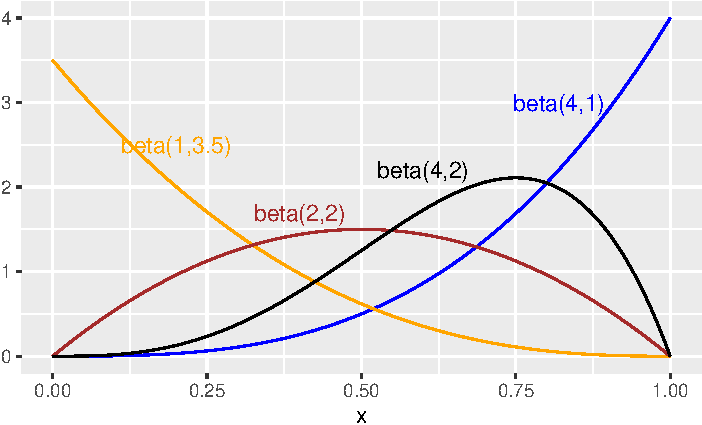
\includegraphics[keepaspectratio]{math340-notes_files/figure-latex/unnamed-chunk-24-1.pdf}}
\caption{\label{fig:unnamed-chunk-24}Nail gun velocity distribution}
\end{figure}

The kinetic energy \(K\) associated with a nail having mass \(m\) moving at velocity \(V\) is \(K = \frac{1}{2}mV^2\). What is \(E(K)\)?

\begin{align*}
E(K) &= E(\frac{1}{2}mV^2)\\
      &= \frac{1}{2}m E(V^2) \\
      &= \frac{1}{2}m (\sigma_V^2 + \mu_V^2)
\end{align*}
Since \(V\) is gamme(4,500), \(\mu_V = 4 \cdot 500 = 2000\) (as we were told) and \(\sigma_V = 4\cdot 500^2,\)
so \[E(K) = 2500000m \text{ units}.\]
\end{example}

\chapter{Central Limit Theorem}\label{central-limit-theorem}

\section{Sums of Random Variables}\label{sums-of-random-variables}

Suppose \(X_1, X_2, \ldots, X_n\) are random variables defined via a random sample of size \(n\) taken from a distribution that is \(N(\mu,\sigma)\).

After the sample is chosen, each \(X_i = x_i\) takes on a value (lower case corresponds to data, upper case corresponds to random variable).
We may then compute the sample mean \[\overline{x} = \frac{1}{n}\sum_{i=1}^n x_i.\]
Prior to picking our actual sample we can consider the function of the random variables \[\overline{X} = \frac{1}{n} \sum_{i=1}^n X_i.\]

\begin{theorem}
\protect\hypertarget{thm:normal-random-sample}{}\label{thm:normal-random-sample}If \(X_1, X_2, \ldots, X_n\) represents a random sample taken from a \(N(\mu,\sigma)\) distribution, then \[\overline{X} = \frac{1}{n} \sum_{i=1}^n X_i ~\text{ is }~ N\left(\mu,\frac{\sigma}{\sqrt{n}}\right).\]
\end{theorem}

\begin{proof}
This theorem is an immediate consequence of Theorem \ref{thm:sum-of-normal-rvs} where each \(a_i = 1/n\).
\end{proof}

\begin{example}
\protect\hypertarget{exm:house-finch}{}\label{exm:house-finch}Let \(X\) equal the duration of a randomly selected song (in seconds) for a house finch. Suppose \(X\) is normal with unknown mean \(\mu\) (we're trying to get a handle on this) and standard deviation \(\sigma = 30\) seconds (somehow we know this). A random sample of 25 song durations is observed. Find the probability that the sample mean will be within 5 seconds of the population mean \(\mu\).

If \(X_1, X_2, \ldots, X_{25}\) denote the 25 song lengths to be observed, each \(X_i \sim N(\mu,30),\) so \[\overline{X} \sim N\left(\mu,\frac{30}{\sqrt{25}}\right) = N(\mu,6).\]
We want to know \[P(|\overline{X}-\mu| < 5).\]
\begin{align*}
P(|\overline{X}-\mu| < 5) &= P(-5 < \overline{X}-\mu < 5)\\
                          &= P\left(\frac{-5}{6} < \frac{\overline{X}-\mu}{6} < \frac{5}{6}\right)\\
                          &= P(-5/6 < Z < 5/6).
\end{align*}
Using R, \(P(-5/6 < Z < 5/6)\) = \texttt{pnorm(5/6)-pnorm(-5/6)} = 0.595.

A secondary question: How big a sample we we need so that the likelihood of the sample mean being within 5 seconds of \(\mu\) is up to .95?

In this case, we want \(n\) so that
\[P\left(\frac{-5}{30/\sqrt{n}} < Z < \frac{5}{30/\sqrt{n}}\right) = .95.\]
Equivalently, we want to find \(n\) so that \[P\left(Z < \frac{-5}{30/\sqrt{n}}\right) = .025.\]
In \(N(0,1),\) \texttt{qnorm(.025)} = -1.96, which means \(P(Z < -1.96) = .025\).
So we want \[\frac{-5}{30/\sqrt{n}} = -1.96,\] and solving for \(n\) and rounding up yields \(n = 139\).
\end{example}

\begin{theorem}
\protect\hypertarget{thm:sample-variance-chisq}{}\label{thm:sample-variance-chisq}Let \(X_1, X_2, \ldots, X_n\) represent a random sample from a \(N(\mu,\sigma)\) distribution, and \[\overline{X} = \frac{1}{n} \sum_{i=1}^n X_i ~~~ \text { and } ~~~ S^2 = \frac{1}{n-1}\sum_{i=1}^n (X_i - \overline{X})^2.\] Then \[\frac{n-1}{\sigma^2}S^2 \sim \chi^2(n-1),\] and \(\overline{X}\) and \(S^2\) are independent random variables.
\end{theorem}

We refer to \(\overline{X}\) and \(S^2\) as the sample mean and sample variance associated with the random sample.

Suppose we draw a sample of size \(n = 25\) from a \(N(10,2)\) distribution. In this case the preceding two theorems tell us that

\begin{itemize}
\tightlist
\item
  \(\overline{X} \sim N(10,2/\sqrt{25}) = N(10,0.4)\)
\item
  \(6 S^2 \sim \chi^2(24)\) (since \(\frac{n-1}{\sigma^2} = 6\) in this case)
\item
  \(\overline{X}\) and \(S^2\) are independent random variables.
\end{itemize}

Let's look at a simulation in R to investigate these statements. The simulation works like this:

\begin{enumerate}
\def\labelenumi{\arabic{enumi}.}
\tightlist
\item
  Draw a random sample of size \(25\) from \(N(10,2)\)
\item
  Calculate \(\overline{x}\) and \(s^2\) from this sample.
\item
  Repeat steps 1 and 2 for many trials, and then consider
\end{enumerate}

\begin{verbatim}
- a frequency plot for $\overline{x}$ (does it look $N(10,0.4)$) 
- a frequency plot for $\frac{n-1}{\sigma^2}s^2$ (does it look $\chi^2(24)$?)
- a scatter plot of $\overline{x}$ against $s^2$ (do they look independent?)
\end{verbatim}

\begin{Shaded}
\begin{Highlighting}[]
\NormalTok{trials }\OtherTok{=} \DecValTok{10000}
\NormalTok{n }\OtherTok{=} \DecValTok{25}\NormalTok{; mu }\OtherTok{=} \DecValTok{10}\NormalTok{; sigma }\OtherTok{=} \DecValTok{2} \CommentTok{\#define sample size and parameters}
\NormalTok{sample\_means }\OtherTok{=} \FunctionTok{c}\NormalTok{() }\CommentTok{\#stores mean of each sample}
\NormalTok{sample\_var }\OtherTok{=} \FunctionTok{c}\NormalTok{() }\CommentTok{\#stores variance of each sample}
\ControlFlowTok{for}\NormalTok{ (i }\ControlFlowTok{in} \DecValTok{1}\SpecialCharTok{:}\NormalTok{trials)\{}
\NormalTok{  x }\OtherTok{=} \FunctionTok{rnorm}\NormalTok{(n,mu,sigma) }\CommentTok{\#draw sample}
\NormalTok{  sample\_means[i] }\OtherTok{=} \FunctionTok{mean}\NormalTok{(x) }\CommentTok{\#record sample mean}
\NormalTok{  sample\_var[i] }\OtherTok{=} \FunctionTok{var}\NormalTok{(x) }\CommentTok{\#record sample variance}
\NormalTok{\}}
\end{Highlighting}
\end{Shaded}

Plots:
\pandocbounded{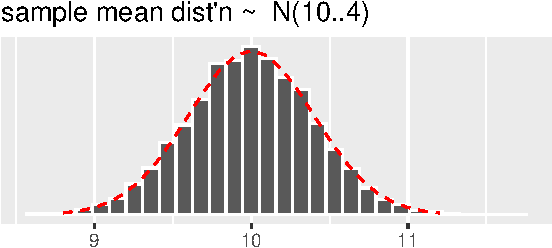
\includegraphics[keepaspectratio]{math340-notes_files/figure-latex/unnamed-chunk-26-1.pdf}}

\pandocbounded{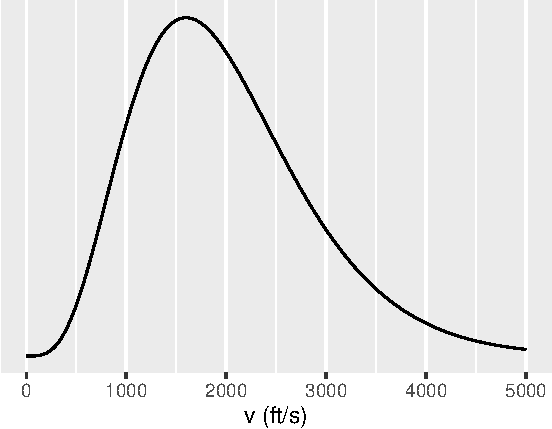
\includegraphics[keepaspectratio]{math340-notes_files/figure-latex/unnamed-chunk-27-1.pdf}}

The scatter plot below suggests no real association between \(\overline{x}\) and \(s^2\).

\pandocbounded{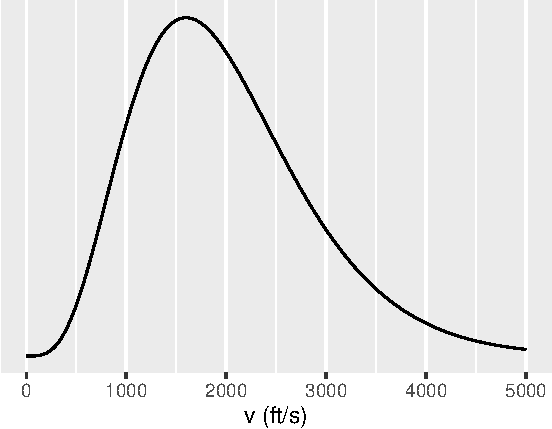
\includegraphics[keepaspectratio]{math340-notes_files/figure-latex/unnamed-chunk-28-1.pdf}}

\section{T distribution}\label{t-distribution}

\begin{definition}
\protect\hypertarget{def:t-distribution}{}\label{def:t-distribution}Let \(Z \sim N(0,1)\) and \(W \sim \chi^2(\nu)\). If \(Z\) and \(W\) are independent then \[\frac{Z}{\sqrt{W/\nu}}\] is said to have a \textbf{t distribution with \(\nu\) degrees of freedom.}\index{t distirbution}
\end{definition}

Here's our motivation for looking at such a thing. Look again at the house finch example (Example \ref{exm:house-finch}). We took a sample of 25 song lengths to estimate \(\mu,\) or rather the likelihood that \(\overline{x}\) is within 5 seconds of \(\mu,\) the population mean. In our solution we assumed we know \(\sigma\). It is perhaps not reasonable to assume we know \(\sigma\) when we're trying to estimate \(\mu\)!

So, if we don't know \(\sigma,\) can we estimate it from the sample? Sure! How about estimating \(\sigma\) with \(s,\) the sample standard deviation?

Now, recall in our solution there came a point when we considered a \(Z\)-score:
\[z = \frac{\overline{x}-\mu}{\sigma/\sqrt{n}}.\]
If we don't know \(\sigma\) can we replace it with the estimate \(s\)?
Good question! Check this out:

From Theorem \ref{thm:standardizing-normal-distributions} \(\displaystyle Z =\frac{ \overline{X}-\mu}{\sigma/\sqrt{n}}\) is \(N(0,1)\)

From Theorem \ref{thm:sample-variance-chisq}, \(\displaystyle\frac{(n-1)S^2}{\sigma^2}\) is \(\chi^2(n-1),\)

So the ratio \(\displaystyle\frac{Z}{\sqrt{\frac{(n-1)S^2}{\sigma^2}\big/(n-1)}}\) has a t distribution with \((n-1)\) degrees of freedom!

Finally, observe
\begin{align*}
  \frac{Z}{\sqrt{\frac{(n-1)S^2}{\sigma^2}\big/(n-1)}} &= \frac{\frac{\overline{X}-\mu}{\sigma/\sqrt{n}}}{s/\sigma} \\
  &= \frac{\overline{X}-\mu}{\sigma/\sqrt{n}} \cdot (\sigma/s) \\
  &= \frac{\overline{X}-\mu}{s/\sqrt{n}}.
\end{align*}

The point of this story is this:

If \(X_1,X_2,\ldots, X_n\) represents a random sample drawn from \(N(\mu,\sigma)\) then

\begin{itemize}
\tightlist
\item
  \(\displaystyle \overline{X} \sim N(\mu,\sigma/\sqrt{n})\)
\item
  so \(\displaystyle Z = \frac{\overline{X}-\mu}{\sigma/\sqrt{n}}\) is \(N(0,1)\)
\item
  while \(\displaystyle T = \frac{\overline{X}-\mu}{s/\sqrt{n}}\) is a t distribution with \(n-1\) degrees of freedom.
\end{itemize}

We denote a \(t\) distributioin with \(k\) degrees of freedom by \(t(k)\). The density function for a \(t(k)\) distribution, defined for all \(-\infty < t < \infty,\) is
\[f(t) = \frac{\Gamma(\frac{k+1}{2})}{\sqrt{k\pi}\Gamma(k/2)}\left(1+\frac{t^2}{2}\right)^{-\left(\frac{k+1}{2}\right)}\]

Suppose \(T \sim t(k)\).

\textbf{Facts about T}:

\begin{enumerate}
\def\labelenumi{\arabic{enumi}.}
\tightlist
\item
  \(E(T) = 0\)
\item
  The distribution has mode at 0
\item
  The distribution is symmetric about the \(y\)-axis
\item
  it has fatter tails than \(N(0,1),\) i.e.,for \(a > 0,\) \(P(t > a) > P(Z > a)\).
\item
  As \(k \to \infty,\) \(t(k) \to N(0,1)\).
\end{enumerate}

\begin{figure}
\centering
\pandocbounded{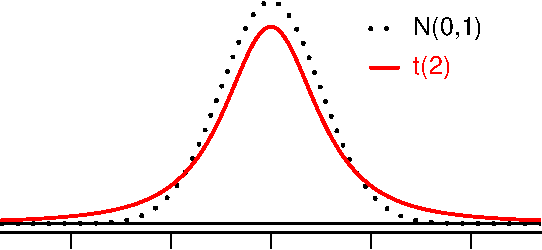
\includegraphics[keepaspectratio]{math340-notes_files/figure-latex/t-vs-st-norm-1.pdf}}
\caption{\label{fig:t-vs-st-norm}A t distribution and N(0,1)}
\end{figure}

\begin{example}
\protect\hypertarget{exm:t-distribution-practice}{}\label{exm:t-distribution-practice}A forester studying the effects of fertilization on certain pine forests is interested in estimating the average basal area (in ft\(^2\)) of pine trees.
Let \(X_1, X_2, \ldots, X_9\) denote a random sample of size 9, and suppose \(X_i \sim N(\mu,\sigma)\) with \(\mu,\) \(\sigma\) unknown.

Find two statistics (i.e., functions of the data) \(g_1\) and \(g_2\) such that \[P(g_1 \leq \overline{X}-\mu \leq g_2) = .9.\]
(The statistics \(g_1\) and \(g_2\) thus give us a range of values we believe with probability .9 captures \(\mu\).)

Well, the statistic \[T = \frac{\sqrt{n}(\overline{X}-\mu)}{S}\] lives in a \(t(8)\) distribution.

Now \(t(8)\) is plotted in figure \ref{fig:t8}, and we can find constants \(c\) and \(-c\) such that the shaded area between them is 0.9.

\begin{figure}
\centering
\pandocbounded{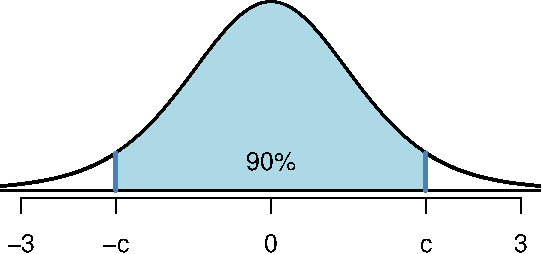
\includegraphics[keepaspectratio]{math340-notes_files/figure-latex/t8-1.pdf}}
\caption{\label{fig:t8}Finding the middle 90\% of a t(8) distribution}
\end{figure}

Using R, in which the t distribution is aptly named as \texttt{t}, \(c\) and \(-c\) are readily found with \texttt{qt()}:

\begin{Shaded}
\begin{Highlighting}[]
\FunctionTok{qt}\NormalTok{(.}\DecValTok{95}\NormalTok{,}\DecValTok{8}\NormalTok{) }\CommentTok{\#gives c}
\end{Highlighting}
\end{Shaded}

\begin{verbatim}
## [1] 1.859548
\end{verbatim}

So \[P(-1.86 < T < 1.86) = .9,\]
where \(T = 3(\overline{X}-\mu)/S,\) and this allows us to solve the problem:

\begin{align*}
.9 &= P(-1.86 < T < 1.86)\\
    &= P(-1.86 < 3(\overline{X}-\mu)/S < 1.86) \\
    &= P(\frac{-1.86}{3}S < \overline{X}-\mu < \frac{1.86}{3}S )\\
    &= P(-.62 S < \overline{X}-\mu < .62 S)
\end{align*}

So \(g_1 = -.62S\) and \(g_2 = .62S\) work!

In practice, this means that, once we have gathered our data of size \(n = 9,\) it is ``likely'' that \(\mu\) is captured by the interval \[(\overline{X} - .62S, \overline{X} + .62S).\]

For instance, suppose our data is (units are ft\(^2\))

\begin{Shaded}
\begin{Highlighting}[]
\NormalTok{data }\OtherTok{=} \FunctionTok{c}\NormalTok{(}\FloatTok{85.5}\NormalTok{,}\FloatTok{71.4}\NormalTok{,}\FloatTok{60.4}\NormalTok{,}\FloatTok{70.9}\NormalTok{,}\FloatTok{78.3}\NormalTok{,}\FloatTok{67.9}\NormalTok{,}\FloatTok{65.3}\NormalTok{,}\FloatTok{63.1}\NormalTok{,}\FloatTok{68.4}\NormalTok{)}
\NormalTok{xbar }\OtherTok{=} \FunctionTok{mean}\NormalTok{(data)}
\NormalTok{s }\OtherTok{=} \FunctionTok{sd}\NormalTok{(data)}
\end{Highlighting}
\end{Shaded}

It is ``likely'' that \(\mu\) falls between \texttt{xbar-.62*s} = 65.3 ft\(^2\) and \texttt{xbar-.62*s} = 74.9 ft\(^2\).
\end{example}

The Central Limit Theorem says, roughly, that even if the underlying population is not normally distributed, it is still reasonable to follow this procedure to estimate \(\mu\).

\section{The Central Limit Theorem}\label{the-central-limit-theorem}

\begin{theorem}[Central Limit Theorem]
\protect\hypertarget{thm:clt}{}\label{thm:clt}Let \(X_1, X_2, \ldots, X_n\) be independent and identically distributed random variables with \(E(X_i) = \mu\) and \(V(X_i) = \sigma^2\) for \(i = 1,2,\ldots,n\). Let \[\overline{X} = \frac{1}{n}\sum_{i=1}^n X_i ~~~ \text{ and } ~~~ U_n = \frac{\overline{X}-\mu}{\sigma/\sqrt{n}}.\]
Then the distribution function of \(U_n\) converges to a standard normal distribution function as \(n \to \infty\).
\end{theorem}

The Central Limit Theorem (CLT) is the mathematical basis for the statistical analysis coming in the next chapter.

\emph{Sketch of Proof}

TODO

\begin{example}[Practical Use of the CLT]
\protect\hypertarget{exm:clt-use}{}\label{exm:clt-use}For large \(n,\) \[\frac{\overline{X}-\mu}{\sigma/\sqrt{n}} \sim N(0,1)\] for a random sample taken from any distribution.
That is, for any distribution (Poisson, binomial, gamma, uniform, \ldots) with mean \(\mu\) and standard deviation \(\sigma,\) if we take a simple random sample (SRS) of decent size, compute the sample mean, then this mean lives in a distribution that is approximately \(N(\mu,\sigma/\sqrt{n})\). Consequently, \[\frac{\overline{X}-\mu}{S/\sqrt{n}}\] will be approximately \(t(n-1)\).
\end{example}

\begin{example}[Can we really walk straight?]
\protect\hypertarget{exm:walk-straight}{}\label{exm:walk-straight}Data on cadence (strides/sec) from a 1992 \href{https://onlinelibrary.wiley.com/doi/10.1002/ajpa.1330890104}{article} in the American Journal of Physical Anthropology, for a sample of size \(n = 20\) ``randomly selected healthy men.''

\begin{Shaded}
\begin{Highlighting}[]
\NormalTok{data }\OtherTok{=} \FunctionTok{c}\NormalTok{(}\FloatTok{0.95}\NormalTok{, }\FloatTok{0.85}\NormalTok{, }\FloatTok{0.92}\NormalTok{, }\FloatTok{0.95}\NormalTok{, }\FloatTok{0.93}\NormalTok{, }\FloatTok{0.86}\NormalTok{, }\FloatTok{1.00}\NormalTok{, }\FloatTok{0.92}\NormalTok{, }\FloatTok{0.85}\NormalTok{, }\FloatTok{0.81}\NormalTok{,}
\FloatTok{0.78}\NormalTok{, }\FloatTok{0.93}\NormalTok{, }\FloatTok{0.93}\NormalTok{, }\FloatTok{1.05}\NormalTok{, }\FloatTok{0.93}\NormalTok{, }\FloatTok{1.06}\NormalTok{, }\FloatTok{1.06}\NormalTok{, }\FloatTok{0.96}\NormalTok{, }\FloatTok{0.81}\NormalTok{, }\FloatTok{0.96}\NormalTok{)}
\end{Highlighting}
\end{Shaded}

The sample mean and standard deviation for these data are

\begin{itemize}
\tightlist
\item
  \(\overline{x}\) = 0.925
\item
  \(s\) = 0.081.
\end{itemize}

We know that \(T = \frac{\overline{X}-\mu}{S/\sqrt{n}}\) has a t(19) distribution (assuming the underlying population is normal), and we can find \(c\) such that \[P(|(\overline{x}-\mu)/(s/\sqrt{n})| < c) = .95.\]
\end{example}

\section{Normal Approximation to a binomial distribution}\label{normal-approximation-to-a-binomial-distribution}

If \(X\) is binom\((n,p),\) we can view \(X\) as a sum of Bernoulli random variables:
\(X = \sum_{i=1^n}Y_i\) where each \(Y_i\) is binom\((1,p)\), which means \(P(Y_i = 1) = p,\) \(P(Y_i = 0) = 1-p,\) and \[\mu_{Y_i} = p ~~~\text{ and } ~~~ \sigma_{Y_i} = \sqrt{p(1-p)}.\]

Note also that \[\frac{1}{n}X = \frac{1}{n}\sum_{i=1}^n Y_i,\] so by the Central Limit Theorem, for large \(n,\) it follows that \(\frac{1}{n}X\) is approximately \(N(p,\sqrt{p(1-p)/n})\). In short:

\begin{quote}
If \(X\) is \(\text{binom}(n,p)\) then \(X\) is approximately \(N(np, \sqrt{np(1-p)})\) for large \(n\).
\end{quote}

Let's look at an example and then fine tune the approximation with a continuity correction.

\begin{example}
Suppose 44\% of a voting population actually plan to vote for candidate A (though we don't know this :)). If we draw a random sample of \(n = 100\) voters, what is the approximate probability that 51 or more of the 100 sampled voters plan to vote for candidate A?

If we know the size of the population we can answer this question precisely with the hypergeometric distribution:

For instance, suppose the population consists of 10000 voters, and \(X\) equals the number of voters in a sample of size 100 that plan to vote for candidate A. Then for any \(x = 0, 1, \ldots, 100,\)
\[p(x) = \frac{\binom{4400}{x}\binom{5600}{100-x}}{\binom{10000}{100}},\]
and \[P(X \geq 51) = \sum_{x = 51}^{100} p(x),\]
and this sum can be calculated in R by:

\begin{Shaded}
\begin{Highlighting}[]
\DecValTok{1}\SpecialCharTok{{-}}\FunctionTok{phyper}\NormalTok{(}\DecValTok{50}\NormalTok{,}\DecValTok{4400}\NormalTok{,}\DecValTok{5600}\NormalTok{,}\DecValTok{100}\NormalTok{)}
\end{Highlighting}
\end{Shaded}

\begin{verbatim}
## [1] 0.09442696
\end{verbatim}

about a 9.4\% chance.

Notice, if the populatioin is just 1000, the answer to this question would be \texttt{1-phyper(50,440,560,100)} = 0.0840868.

If we don't know the size of the population, but assume it's big, then the sampling process is close to that of 100 identical Bernoulli trials, where in each case, \(p = .44\). In this case, \(X\) is \(\text{binom}(n=100,p=.44),\) and \(P(X \geq 51)\) is found in R via

\begin{Shaded}
\begin{Highlighting}[]
\DecValTok{1}\SpecialCharTok{{-}}\FunctionTok{pbinom}\NormalTok{(}\DecValTok{50}\NormalTok{,}\DecValTok{100}\NormalTok{,.}\DecValTok{44}\NormalTok{)}
\end{Highlighting}
\end{Shaded}

\begin{verbatim}
## [1] 0.09553862
\end{verbatim}

Notice that the binomial approximation here is closer to the actual probability calculated with the hypergeometric distribution for \(n = 10000\) than for \(n = 1000\).

Finally, let's approximate the likelihood with a normal distribution.
According to the Central Limit Theorem, \(X\) is approximately \(N(44,\sqrt{100(.44)(.56)}),\) or \(N(44,4.964)\).
So \(P(X \geq 51) = 1 - P(X < 51)\) = \texttt{1\ -\ pnorm(51,44,4.964)} = 0.079.

This normal estimate is a little low, and we can improve the estimate by making what is called a \emph{continuity correction}.
\end{example}

\subsection*{Continuity Correction}\label{continuity-correction}
\addcontentsline{toc}{subsection}{Continuity Correction}

Suppose \(X\) is \(\texttt{binom}(100,.44),\) as in the voting example, and we want to estimate \(P(51 \leq X \leq 55)\) by using the normal approximation \(N(44,\sqrt{100(.44)(.56)})\).

The actual binomial probability can be represented as the sum of the 5 rectangle areas in Figure \ref{fig:continuity-correction}.
Each rectangle has width 1, and the heights of the rectangles correspond to \(P(X = x)\) (binomial probability) for each \(x = 51,\ldots,55.\)
We also see in the figure a portion of the \(N(44,\sqrt{100(.44)(.56)})\) density curve \(f(x)\). The area under \(f\) that best approximates the rectangle areas will be the integral with bounds {[}50.5,55.5{]} (whose area is shaded in the figure), as opposed to the integral with bounds {[}51,55{]}.

\begin{figure}
\centering
\pandocbounded{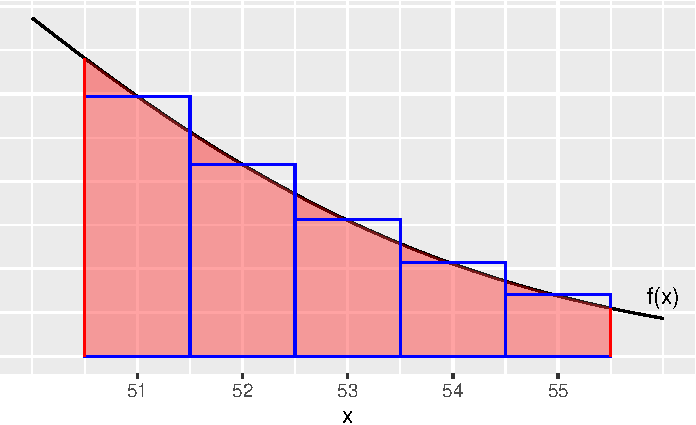
\includegraphics[keepaspectratio]{math340-notes_files/figure-latex/continuity-correction-1.pdf}}
\caption{\label{fig:continuity-correction}Continuity correction to estimate a binomial probability with a normal curve}
\end{figure}

In other words, to better approximate \(P(51\leq X \leq 55)\) with a normal distribution, instead of evaluating \(\int_{51}^{55} f(x)~dx,\) we should use a continuity correction\index{continuity correction} and evaluate \[\int_{50.5}^{55.5} f(x)~dx.\]

Observe:

\begin{itemize}
\tightlist
\item
  Actual value of \(P(51\leq X \leq 55)\):

  \begin{itemize}
  \tightlist
  \item
    \texttt{sum(dbinom(51:55,100,.44))} = 0.08503
  \end{itemize}
\item
  Normal approximation without continuity correction:

  \begin{itemize}
  \tightlist
  \item
    \texttt{pnorm(55,44,4.964)-pnorm(51,44,4.964)} = 0.0659
  \end{itemize}
\item
  Normal approximation with continuity correction:

  \begin{itemize}
  \tightlist
  \item
    \texttt{pnorm(55.5,44,4.964)-pnorm(50.5,44,4.964)} = 0.08493
  \end{itemize}
\end{itemize}

Now, we return to our voting example and the normal approximation to the probability that at least 51 people in a sample of 100 people will vote for candidate \(A\). With a continuity correction, \(P(X \geq 51)\) is better approximated with:

\begin{Shaded}
\begin{Highlighting}[]
\FunctionTok{pnorm}\NormalTok{(}\FloatTok{100.5}\NormalTok{,}\DecValTok{44}\NormalTok{,}\FloatTok{4.964}\NormalTok{)}\SpecialCharTok{{-}}\FunctionTok{pnorm}\NormalTok{(}\FloatTok{50.5}\NormalTok{,}\DecValTok{44}\NormalTok{,}\FloatTok{4.964}\NormalTok{)}
\end{Highlighting}
\end{Shaded}

\begin{verbatim}
## [1] 0.09519473
\end{verbatim}

Here's one more example.

\begin{example}
Use continuity correction to estimate \(P(460 \leq X \leq 480)\) if \(X\) is \(\texttt{binom}(1000,.5)\).

Well, with a continuity correction
\[P(460 \leq X \leq 480) \approx P(459.5 \leq Y \leq 480.5),\] where \(Y \sim N(500,\sqrt{1000(.5)(.5)})\).

\begin{itemize}
\tightlist
\item
  Actual probability: \texttt{pbinom(480,1000,.5)-pbinom(460,1000,.5)} = 0.1025.
\end{itemize}

Estimated probability: \texttt{pnorm(480.5,500,sqrt(250))-pnorm(459.5,500,sqrt(250))} = 0.1035.
\end{example}

\chapter{Estimation}\label{estimation}

\textbf{The Scene}: We want to estimate some parameter \(\theta\) of a population by gathering and analyzing an independent random sample drawn from the population.

\section{Unbiased Estimators}\label{unbiased-estimators}

\begin{definition}
\protect\hypertarget{def:statistic}{}\label{def:statistic}A \textbf{statistic}\index{statistic} is any function of a random sample \(X_1, X_2, \ldots X_n\) drawn from a population.
\end{definition}

\begin{definition}
A statistic \(\hat{\theta}\) based on a random sample \(X_1, X_2, \ldots X_n\) is an \textbf{unbiased estimator}\index{estimator!unbiased} of the population parameter \(\theta\) if \(E(\hat{\theta}) = \theta\).

The \textbf{bias of \(\hat{\theta}_n\)}\index{estimator!bias of} is \(B(\hat{\theta}) = E(\hat{\theta})-\theta\).

The \textbf{mean square error of \(\hat{\theta}_n\)}\index{estimator!mean square error of} is MSE\((\hat{\theta}) = E[(\hat{\theta}-\theta)^2]\).
\end{definition}

A \emph{good} estimator for the parameter \(\theta\) is a statistic \(\hat{\theta}\) that is unbiased with variance as small as possible. These features of \(\hat{\theta}\) would ensure that for any random sample you happen to gather, the value \(\hat{\theta}\) you compute from the data is likely to be close to \(\theta\) (or at least likelier to be close to \(\theta\) than some other statistic).

\begin{example}[Two unbiased estimators for the upper bound of a uniform distribution]
\protect\hypertarget{exm:estimating-uniform-parameter}{}\label{exm:estimating-uniform-parameter}Suppose \(X_1, X_2, \ldots, X_n\) is an independent random sample drawn from a uniform distribution \(U(0,\theta),\) where \(\theta\) is unknown.
So each \(X_i\) is a random real number between 0 and \(\theta\).

\begin{quote}
How can we estimate the unknown parameter \(\theta\) from the data?
\end{quote}

\textbf{First estimator}: Create an estimator from the sample mean: \[\overline{X} = \frac{1}{n}\sum_{i = 1}^n X_i.\]

By properties of expected value,
\begin{align*}
E(\overline{X}) &= \frac{1}{n}\sum_{i = 1}^n E(X_i) \\
                &= \frac{1}{n}\sum_{i = 1}^n \frac{\theta}{2}
\end{align*}
since each \(X_i\) is \(U(0,\theta),\) so \(E(X_i) = \frac{0 + \theta}{2}\).

It follows that \[E(\overline{X}) = \frac{1}{n} \cdot n \cdot \frac{\theta}{2} = \frac{\theta}{2}.\]

Since \(E(\overline{X}) \neq \theta,\) the sample mean \(\overline{X}\) is not an unbiased estimator for \(\theta\). This makes sense. We shouldn't expect the average of the random numbers to be a good estimate of the upper bound of the interval from which the numbers were picked.

However, \(E(\overline{X})\) \emph{does} equal \textbf{a constant multiple} of \(\theta,\) which means we can easily adjust \(\overline{X}\) to a statistic that \emph{is} an unbiased estimator for \(\theta\):

\[\hat{\theta}_1 = 2\overline{X} \tag{unbiased estimator 1}\]
\textbf{Second Estimator}: Create an estimator from the maximum value of the data, since this max is ``closest'' to \(\theta\) of all the data points.

Let \(Y = \max\{X_1, X_2, \ldots, X_n\}.\) We prove below in \ref{order-statistics} that \[E(Y) = \frac{n}{n+1}\theta.\]
Assuming that for now, we can say that \[\hat{\theta}_2 = \frac{n+1}{n}\cdot Y \tag{unbiased estimator 2}\] is also an unbiased estimator for \(\theta\).

Let's see how these different estimators do for a particular random sample generated in R.

\begin{Shaded}
\begin{Highlighting}[]
\NormalTok{theta }\OtherTok{=} \DecValTok{20} \CommentTok{\# we pretend we don\textquotesingle{}t know this parameter}
\NormalTok{n }\OtherTok{=} \DecValTok{10} \CommentTok{\# the size of the sample}
\NormalTok{X }\OtherTok{=} \FunctionTok{runif}\NormalTok{(n,}\DecValTok{0}\NormalTok{,theta) }\CommentTok{\# generate the random sample}
\NormalTok{est\_1 }\OtherTok{=} \DecValTok{2}\SpecialCharTok{*}\FunctionTok{mean}\NormalTok{(X)}
\NormalTok{est\_2 }\OtherTok{=}\NormalTok{ (n}\SpecialCharTok{+}\DecValTok{1}\NormalTok{)}\SpecialCharTok{/}\NormalTok{n}\SpecialCharTok{*}\FunctionTok{max}\NormalTok{(X)}
\FunctionTok{print}\NormalTok{(}\FunctionTok{round}\NormalTok{(X,}\DecValTok{2}\NormalTok{))}
\end{Highlighting}
\end{Shaded}

\begin{verbatim}
##  [1]  5.20 10.78 11.71 18.49 19.50 16.97  2.50  1.03  2.95 14.35
\end{verbatim}

For this single sample the estimators takes on these values:

\begin{itemize}
\tightlist
\item
  Estimator 1: \(\hat{\theta}_1\) = 20.7
\item
  Estimator 2: \(\hat{\theta}_2\) = 21.5.
\end{itemize}

The fact that both estimators are unbiased means that in the long run, the average of all the \(\hat{\theta}_1\) estimates would approach \(\theta,\) and the same is true for the average of the \(\hat{\theta}_2\) estimates.

So, they're both good estimaors of \(\theta\) in that regard. What makes one estimator better is if the \emph{variation} of the estimates obtained from repeated sampling is smaller for one than the other.

Let's simulate drawing 1000 different samples of size \(n = 10,\) recording the distribution of values taken by the estimates \(\theta_1\) and \(\theta_2,\) and seeing which distribution has smaller variance.

\begin{Shaded}
\begin{Highlighting}[]
\NormalTok{theta }\OtherTok{=} \DecValTok{20}\NormalTok{;n }\OtherTok{=} \DecValTok{10} \CommentTok{\# the size of the sample in each trial}
\NormalTok{trials }\OtherTok{=} \DecValTok{1000} \CommentTok{\# number of times we take a sample of size n}
\NormalTok{dist\_1 }\OtherTok{=} \FunctionTok{c}\NormalTok{() }\CommentTok{\# records estimator 1 values}
\NormalTok{dist\_2 }\OtherTok{=} \FunctionTok{c}\NormalTok{() }\CommentTok{\# records estimator 2 values}
\CommentTok{\# run the trials}
\ControlFlowTok{for}\NormalTok{ (i }\ControlFlowTok{in} \DecValTok{1}\SpecialCharTok{:}\NormalTok{trials)\{}
\NormalTok{  X }\OtherTok{=} \FunctionTok{runif}\NormalTok{(n,}\DecValTok{0}\NormalTok{,theta) }\CommentTok{\# generate the random sample}
\NormalTok{  dist\_1[i] }\OtherTok{=} \DecValTok{2}\SpecialCharTok{*}\FunctionTok{mean}\NormalTok{(X)}
\NormalTok{  dist\_2[i] }\OtherTok{=}\NormalTok{ (n}\SpecialCharTok{+}\DecValTok{1}\NormalTok{)}\SpecialCharTok{/}\NormalTok{n}\SpecialCharTok{*}\FunctionTok{max}\NormalTok{(X)}
\NormalTok{\}}
\CommentTok{\# create data frame of results for ggplot}
\NormalTok{df }\OtherTok{=} \FunctionTok{rbind}\NormalTok{(}\FunctionTok{data.frame}\NormalTok{(}\AttributeTok{estimator =} \StringTok{"1"}\NormalTok{,}\AttributeTok{value =}\NormalTok{ dist\_1),}
           \FunctionTok{data.frame}\NormalTok{(}\AttributeTok{estimator =} \StringTok{"2"}\NormalTok{,}\AttributeTok{value =}\NormalTok{ dist\_2))}
\CommentTok{\# plot}
\FunctionTok{ggplot}\NormalTok{(df)}\SpecialCharTok{+}
  \FunctionTok{geom\_density}\NormalTok{(}\FunctionTok{aes}\NormalTok{(}\AttributeTok{x=}\NormalTok{value,}\AttributeTok{fill=}\NormalTok{estimator),}\AttributeTok{alpha =}\NormalTok{ .}\DecValTok{4}\NormalTok{)}\SpecialCharTok{+}
  \FunctionTok{theme\_get}\NormalTok{()}
\end{Highlighting}
\end{Shaded}

\pandocbounded{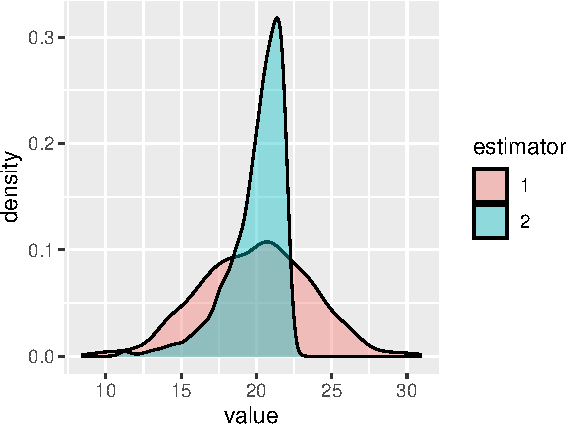
\includegraphics[keepaspectratio]{math340-notes_files/figure-latex/unnamed-chunk-36-1.pdf}}
Both estimators have average value near 20. In fact,

\begin{itemize}
\tightlist
\item
  \texttt{mean(dist\_1)}- = 20
\item
  \texttt{mean(dist\_2)} = 20.01.
\end{itemize}

But the estimator 2 distribution has visibly smaller variance. Indeed,

\begin{itemize}
\tightlist
\item
  \texttt{sd(dist\_1)} = 3.67
\item
  \texttt{sd(dist\_2)} = 1.82.
\end{itemize}

It appears that the better estimator here is the one derived from the maximum value of the data as opposed to the mean of the data.
\end{example}

\section{Order Statistics}\label{order-statistics}

If \(X_1, X_2, \ldots, X_n\) is a sample drawn from a distribution with density function \(f_X(x),\) let \[Y = \text{max}\{X_1, X_2, \ldots, X_n\}.\]
We can deduce the density function for \(Y\) by first writing down the distribution function. For any real number \(y,\)
\begin{align*}
F_Y(y) &= P(Y \leq y) \\
      &= P(\text{all }X_i \leq y) \\
      &= P(X_1 \leq y, X_2 \leq y, \ldots, X_n \leq y) \\
      &= \left[F_X(y)\right]^n.
\end{align*}
We differentiate \(F_Y\) with the chain rule to find \(f_Y\):
Thus, \[f_Y = n\left[F_X(y)\right]^{n-1}\cdot f_X(y). \tag{density for the max of sample}\]
For \(X\) is \(U(0,\theta)\) as in the previous example, \(f_X(x) = 1/\theta,\) and \(F_X(x) = x/\theta,\) for \(0 \leq x \leq \theta\). So, the density function for \(Y = \text{max}(X_i),\) where \(X_i\) is \(U(0,\theta)\) is
\begin{align*}
f_Y(y) &= n \left[\frac{y}{\theta}\right]^{n-1} \cdot \frac{1}{\theta}\\
      &= \frac{n}{\theta^n}y^{n-1},
\end{align*}
for \(0 \leq y \leq \theta,\)
and \[E(Y) = \int_0^\theta y \cdot \frac{n}{\theta^n}y^{n-1}~dy = \cdots = \frac{n}{n+1}\theta,\]
giving us the result we assumed when defining estimator 2 in the previous example.

In the homework you derive the density function for the minimum of a random sample.

\section{Common Unbiased Estimators}\label{common-unbiased-estimators}

We have seen the following strategy for finding unbiased estimators: Try a simple estimator (e.g., \(\overline{X}\) or max\((X_i)\)) and tweak it so that it becomes unbiased.

\subsection{\texorpdfstring{Estimating \(\mu,\) a population mean}{Estimating \textbackslash mu, a population mean}}\label{estimating-mu-a-population-mean}

If \(X_1, X_2, \ldots, X_n\) is a sample drawn from a distribution with mean \(\mu\) and standard deviation \(\sigma\) we have seen that the sample mean \(\overline{X}\) has \(E(\overline{X}) = \mu\) and standard deviation \(\sigma/\sqrt{n}\). That is,

\begin{quote}
\(\overline{X}\) is an unbiased estimator for \(\mu,\) and its standard deviation is \(\sigma/\sqrt{n}\).
\end{quote}

\subsection{\texorpdfstring{Estimating \(p,\) a population proportion}{Estimating p, a population proportion}}\label{estimating-p-a-population-proportion}

If \(X_1, X_2, \ldots, X_n\) is a sample drawn from a \(b(1,n)\) distribution (Bernoulli trial!) and \(X = X_1 + X_2 + \cdots + X_n\) equals the number of successes in \(n\) trials, then we have seen that \(\hat{p} = X/n\) has \(E(\hat{p}) = p\) and standard deviation \(\displaystyle\sqrt{\frac{p(1-p)}{n}}\). That is,

\begin{quote}
\(\hat{p}\) is an unbiased estimator for \(p,\) and its standard deviation is \(\displaystyle\sqrt{\frac{p(1-p)}{n}}\).
\end{quote}

\begin{example}
In a sample of 65 Linfield students, 24 are first-generation students. Estimate \(p,\) the proportion of all Linfield students that are first-generation, and place a 2 standard deviation bound on the error of estimation.

From our sample, our point estimate for \(p\) is \(\hat{p} = 24/65 \approx .369.\) We know by the CLT that \[\hat{p} \sim N(p, \sqrt{p(1-p)/n}),\]
and in a normal distribution, about 95\% of the distribution is within two standard deviations of the mean. In other words,
\[P\left(~|\hat{p}-p|<2\cdot\sqrt{p(1-p)/n}~\right) \approx 0.95.\]
Now we don't know \(p\) (in fact, we're trying to estimate it!), so we can't know the value of the standard deviation \(\sqrt{p(1-p)/n}.\) However, for large \(n,\) the expression \(\sqrt{x(1-x)/n}\) doesn't change much for nearby inputs, except when the inputs are close to 0 or 1 (try it!). In other words, we can reasonably expect \[\sqrt{\hat{p}(1-\hat{p})/n} ~\approx \sqrt{p(1-p)/n},\] in which case we can estimate that
\[P\left(~|\hat{p}-p|<2\cdot\sqrt{\hat{p}(1-\hat{p})/n}~\right) \approx 0.95.\]
In this problem \(\hat{p} \approx .37,\) so \(2 \cdot \sqrt{p(1-p)/n} \approx 0.12,\) so we can say that \[|.37-p| < 0.12\] with probability about .95, and that
\[ .25 < p < .49\] gives a two standard deviation bound on the error of estimation.
\end{example}

\subsection{\texorpdfstring{Estimating \(\mu_1 - \mu_2,\) the difference of two population means}{Estimating \textbackslash mu\_1 - \textbackslash mu\_2, the difference of two population means}}\label{estimating-mu_1---mu_2-the-difference-of-two-population-means}

Suppose we have two independent random samples drawn from distinct normal distributions.

\begin{itemize}
\tightlist
\item
  \(X_1, \ldots, X_{n_1} \sim N(\mu_1,\sigma_1)\)
\item
  \(Y_1, \ldots, Y_{n_2} \sim N(\mu_2, \sigma_2)\)
\end{itemize}

Let \(\overline{X}\) and \(\overline{Y}\) denote the respective sample means, and consider the point estimate \(\overline{X}-\overline{Y}\) of \(\mu_1-\mu_2\).
Since \(\overline{X}-\overline{Y}\) is a linear combination of normal random variables, we can show \(\overline{X}-\overline{Y}\) is itself normal, with

\begin{itemize}
\tightlist
\item
  mean = \(E(\overline{X}-\overline{Y}) = E(\overline{X})-E(\overline{Y}) = \mu_1 - \mu_2\)
\item
  variance = \(V(\overline{X}-\overline{Y}) = V(\overline{X})+V(\overline{Y}) = \frac{\sigma_1^2}{n_1} + \frac{\sigma_2^2}{n_2}\).
\end{itemize}

So \(\overline{X}-\overline{Y}\) is an unbiased estimator for \(\mu_1 - \mu_2\) with standard deviation equal to \(\displaystyle\sqrt{\sigma_1^2/n_1 + \sigma_2^2/n_2}.\)

\subsection{\texorpdfstring{Estimating \(p_1 - p_2,\) the difference of two population proportions}{Estimating p\_1 - p\_2, the difference of two population proportions}}\label{estimating-p_1---p_2-the-difference-of-two-population-proportions}

An unbiased estimator for \(p_1-p_2\) is \(\hat{p}_1-\hat{p}_2,\) where \(\hat{p}_i\) equals the sample proportion from a sample of size \(n_i\) drawn from population \(i\) (which has population proportion \(p_i\)).

One can show that the point estimate \(\hat{p}_1 - \hat{p}_2\) is approximately normal with mean \(p_1-p_2\) and standard deviation \(\displaystyle \sqrt{\frac{p_1(1-p_1)}{n_1}+\frac{p_2(1-p_2)}{n_2}}\) for reasonably sized samples (more on this later). For now lets consider an example.

\begin{example}[Two Large Buckets]
Each of two large buckets is full of two types of marbles, orange and green. Let \(p_i\) denote the proportion of orange marbles in bucket \(i\) (\(i = 1,2\)).

\begin{quote}
Estimate \(p_1-p_2,\) and place a 2 standard deviation bound on the error of estimation.
\end{quote}

\begin{itemize}
\tightlist
\item
  Sample 1: \(n_1 = 120\) marbles from bucket 1, of which 45 are orange, so \(\hat{p}_1 = .375\)
\item
  Sample 2: \(n_2 = 80\) marbles from bucket 2, of which 36 are orange, so \(\hat{p}_2 = .45\).
\end{itemize}

Point estimate: \[\hat{p}_1 - \hat{p}_2 = -.075.\]
Also, it is reasonable to assume that the sampling distribution for \(\hat{p}_1-\hat{p}_2\) is approximately
\[N\left(p_1-p_2, \sqrt{\frac{\hat{p}_1(1-\hat{p}_1)}{n_1}+\frac{\hat{p}_2(1-\hat{p}_2)}{n_2}}\right)\]
(again, plugging in \(\hat{p}_i\) for \(p_i\) in the standard deviation is ``ok'' for larger sample sizes and values of \(\hat{p}_i\) not too close to 0 or 1.).

For a normal distribution, about 95\% of the distribution falls within 2 standard deviations of the mean, so
\[P\left(|(\hat{p}_1-\hat{p}_2)-(p_1-p_2)|< c\right)\approx .95,\]
where \[c = 2\cdot \sqrt{\frac{\hat{p}_1(1-\hat{p}_1)}{n_1}+\frac{\hat{p}_2(1-\hat{p}_2)}{n_2}}.\]

So, we can say that \[\hat{p}_1-\hat{p}_2 - c < p_1 - p_2 < \hat{p}_1-\hat{p}_2 + c\] with probability about .95. Plugging in numbers in this example, we obtain the interval \[-0.217 < p_1 - p_2 < 0.067.\]

Hmm\ldots{} this interval contains 0. While the sample proportions here are such that we may suspect the second bucket has a higher proportion of orange marbles, when we take into account the error of estimation due to sampling variability, our samples do not provide overwhelming evidence that the buckets have different proportions of orange marbles.
\end{example}

\chapter{Confidence Intervals}\label{confidence-intervals}

In many of the examples in Chapter \ref{estimation} we built confidence intervals, interval estimators that specify the method for using a sample to calculate two numbers that form the endpoints of an interval that likely (with some pre-assigned probability) contains the paramter of interest.

\section{Pivotal Quantities}\label{pivotal-quantities}

Here is the general scene for a \textbf{confidence interval}\index{confidence interval} for a parameter \(\theta\). We use a sample to determine the \textbf{lower}\index{confidence interval!lower limit estimator} and \textbf{upper confidence limit estimators}\index{confidence interval!upper limit estimator}, \(\hat{\theta}_L\) and \(\hat{\theta}_U\). If \[P(\hat{\theta}_L \leq \theta \leq \hat{\theta_U}) = 1 - \alpha\] the probability \(1-\alpha\) is called the \textbf{confidence level}\index{confidence interval!confidence level}.

One method for finding confidence intervals is called the \textbf{pivotal method}\index{confidence interval!pivotal method}, which leverages a \textbf{pivotal quantity}\index{pivotal quantity}, which is a quantity with two features:

\begin{enumerate}
\def\labelenumi{\arabic{enumi}.}
\tightlist
\item
  It is a function of the data \(X_1, \ldots, X_n\) and the parameter of interest \(\theta,\) and
\item
  its probability distribution does not depend on \(\theta\).
\end{enumerate}

\begin{example}
If a population mean \(\mu\) is the parameter of interest, and we have sample \(X_1, \ldots, X_n,\) then a good pivotal quantity, assuming \(X_i\) is approximately \(N(\mu,\sigma),\) is \[T = \frac{\overline{X}-\mu}{S/\sqrt{n}}.\] It meets both requirements here: it is a function of the data and the parameter \(\mu,\) and it lives in a \(t(n-1)\) distribution, which is independent of \(\mu\).
\end{example}

\begin{example}
If a population proportion \(p\) is the parameter of interest, and we have sample proportion \(\hat{p}\) (from a sample of size \(n\)), then the pivotal quantity \[Z = \frac{\hat{p}-p}{\sqrt{\hat{p}(1-\hat{p})/n}}\] is approximately \(N(0,1),\) a distribution independent of \(p\).
\end{example}

\begin{example}
Consider \(X_1, \ldots, X_n\) drawn from the uniform distribution \(U(0,\theta)\) and \(Y = \text{max}(X_1, \ldots, X_n)\). We proved in Example \ref{exm:estimating-uniform-parameter} that \[F_Y(y) = \left(\frac{y}{\theta}\right)^n ~~~\text{ and }~~~ f_Y(y) = \frac{n}{\theta^n}y^{n-1},\] for \(0 \leq y \leq \theta\).
Now, let \(U = \frac{1}{\theta}Y,\) which is just a function of the data and \(\theta\).

The distribution function for \(U\) is
\begin{align*}
F_U(u) &= P(U \leq u)\\
      &= P(Y/\theta \leq u)\\
      &= P(Y \leq u\cdot \theta)\\
      &= F_Y(u\theta) \\
      &= \left(\frac{u\theta}{\theta}\right)^n &\text{ for } 0 \leq u \leq 1\\
      &= u^n & \text{ for } 0 \leq u \leq 1,
\end{align*}

which doesn't depend on \(\theta\). So \(U = Y/\theta\) is a pivotal quantity.

Let's use \(U\) to build a 95\% confidence interval for \(\theta\) based on a sample \(X_1, X_2, \ldots, X_n\) drawn from the uniform distribution \(U(0,\theta)\).

In particular, we find estimators \(\hat{\theta}_L\) and \(\hat{\theta}_U\) so that \(P(\hat{\theta}_L \leq \theta \leq \hat{\theta}_U) = .95\).

Well, we know the distribution of the pivotal quantity \(U = Y/\theta,\) where \(Y\) is the max of the data, so one solution here is to find constants \(a\) and \(b\) between 0 and 1 so that

\begin{itemize}
\tightlist
\item
  \(P(U < a) = 0.025\)
\item
  \(P(U > b) = 0.025\)
\end{itemize}

\[.025 = P(U < a) = F_U(a) = a^n \implies a = \sqrt[n]{.025}\]
and
\[.025 = P(U > b) = 1-F_U(b) = 1 - b^n \implies b = \sqrt[n]{.975}.\]
With this we obtain a general form for a 95\% confidence interval for \(\theta\):

\begin{align*}
.95 &= P\left(\frac{1}{\sqrt[n]{.025}} < U < \frac{1}{\sqrt[n]{.975}}\right)\\
    &= P\left(\frac{1}{\sqrt[n]{.025}} < \frac{Y}{\theta} < \frac{1}{\sqrt[n]{.975}}\right)\\
    &= P\left(\frac{1}{\sqrt[n]{.025}} > \frac{\theta}{Y} > \frac{1}{\sqrt[n]{.975}}\right)\\
    &= P\left(\frac{Y}{\sqrt[n]{.975}} < \theta < \frac{Y}{\sqrt[n]{.025}}\right).
\end{align*}

We see that \(\hat{\theta}_L = \frac{Y}{\sqrt[n]{.975}}\) and \(\hat{\theta}_U = \frac{Y}{\sqrt[n]{.025}}\).

Let's put this interval formula to use. Here's a random sample of size 25 drawn in R from a \(U(0,64)\) distribution (though let's pretend we don't actually know \(\theta = 64\) here.)

\begin{Shaded}
\begin{Highlighting}[]
\NormalTok{theta }\OtherTok{=} \DecValTok{64}
\NormalTok{n }\OtherTok{=} \DecValTok{25}
\NormalTok{x }\OtherTok{=} \FunctionTok{runif}\NormalTok{(n,}\DecValTok{0}\NormalTok{,theta)}
\NormalTok{y }\OtherTok{=} \FunctionTok{max}\NormalTok{(x)}
\NormalTok{L }\OtherTok{=}\NormalTok{ y}\SpecialCharTok{/}\NormalTok{(.}\DecValTok{975}\NormalTok{)}\SpecialCharTok{\^{}}\NormalTok{(}\DecValTok{1}\SpecialCharTok{/}\NormalTok{n) }\CommentTok{\#lower bound estimator for 95\% CI}
\NormalTok{U }\OtherTok{=}\NormalTok{ y}\SpecialCharTok{/}\NormalTok{(.}\DecValTok{025}\NormalTok{)}\SpecialCharTok{\^{}}\NormalTok{(}\DecValTok{1}\SpecialCharTok{/}\NormalTok{n) }\CommentTok{\#upper bound estimator for 95\% CI}
\FunctionTok{c}\NormalTok{(L,U) }\CommentTok{\#confidence interval}
\end{Highlighting}
\end{Shaded}

\begin{verbatim}
## [1] 59.25125 68.60253
\end{verbatim}

Did our confidence interval actually capture the value of the parameter (64)?
The confidence level of 95\% gives us confidence that it does, in this sense: If we were to repeat the sampling procedure a large number of times, each time using our new sample to determine a new confidence interval for \(\theta,\) then we should expect about 95\% of the intervals to contain the parameter \(\theta\).

We can check this using R, first writing a little function out of the code above for producing the interval.

\begin{Shaded}
\begin{Highlighting}[]
\NormalTok{conf\_int\_for\_theta }\OtherTok{\textless{}{-}} \ControlFlowTok{function}\NormalTok{(}\AttributeTok{n=}\DecValTok{25}\NormalTok{,}\AttributeTok{theta=}\DecValTok{64}\NormalTok{)\{}
\NormalTok{  x }\OtherTok{=} \FunctionTok{runif}\NormalTok{(n,}\DecValTok{0}\NormalTok{,theta)}
\NormalTok{  y }\OtherTok{=} \FunctionTok{max}\NormalTok{(x)}
\NormalTok{  L }\OtherTok{=}\NormalTok{ y}\SpecialCharTok{/}\NormalTok{(.}\DecValTok{975}\NormalTok{)}\SpecialCharTok{\^{}}\NormalTok{(}\DecValTok{1}\SpecialCharTok{/}\NormalTok{n) }
\NormalTok{  U }\OtherTok{=}\NormalTok{ y}\SpecialCharTok{/}\NormalTok{(.}\DecValTok{025}\NormalTok{)}\SpecialCharTok{\^{}}\NormalTok{(}\DecValTok{1}\SpecialCharTok{/}\NormalTok{n)}
\NormalTok{  check }\OtherTok{=} \FunctionTok{ifelse}\NormalTok{(((L }\SpecialCharTok{\textless{}=}\NormalTok{ theta)}\SpecialCharTok{\&}\NormalTok{(theta }\SpecialCharTok{\textless{}=}\NormalTok{ U)),}\DecValTok{1}\NormalTok{,}\DecValTok{0}\NormalTok{)}\CommentTok{\#1 if interval captures theta, 0 else}
  \FunctionTok{return}\NormalTok{(}\FunctionTok{c}\NormalTok{(L,U,check)) }\CommentTok{\#returns the interval and whether it captured theta}
\NormalTok{\}}

\NormalTok{results }\OtherTok{=} \FunctionTok{c}\NormalTok{() }\CommentTok{\# a vector storing whether interval generated from data captures theta, for 100 trials}
\ControlFlowTok{for}\NormalTok{ (i }\ControlFlowTok{in} \DecValTok{1}\SpecialCharTok{:}\DecValTok{100}\NormalTok{)\{}
\NormalTok{  results[i]}\OtherTok{=}\FunctionTok{conf\_int\_for\_theta}\NormalTok{()[}\DecValTok{3}\NormalTok{]}
\NormalTok{\}}
\FunctionTok{table}\NormalTok{(results)}
\end{Highlighting}
\end{Shaded}

\begin{verbatim}
## results
##  0  1 
##  4 96
\end{verbatim}

In this simulation we drew 100 different random samples of size 25, each time generating a confidence interval for \(\theta\) and found that 96 of the 100 intervals captured \(\theta\). We would expect in the long run that 95\% of such confidence intervals would capture \(\theta\).
\end{example}

We have, generally,

\begin{itemize}
\tightlist
\item
  \textbf{2-sided confidence intervals for \(\theta\)}\index{confidence interval!2-sided}: \([\hat{\theta}_L,\hat{\theta}_U],\) where \(P(\hat{\theta}_L \leq \theta \leq \hat{\theta}_U)=1-\alpha,\)
\item
  \textbf{1-sided confidence intervals for \(\theta\)}\index{confidence interval!1-sided}:

  \begin{itemize}
  \tightlist
  \item
    \([\hat{\theta}_L,\infty),\) where \(P(\hat{\theta}_L \leq \theta)=1-\alpha,\)
  \item
    \((-\infty,\hat{\theta}_U],\) where \(P(\theta \leq \hat{\theta}_U)=1-\alpha\).
  \end{itemize}
\end{itemize}

The interval \([\hat{\theta}_L,\infty)\) is called a \textbf{lower 1-sided} confidence interval, and in this case \(\hat{\theta}_L\) is called the \textbf{lower confidence limit}, and \((-\infty,\hat{\theta}_U]\) is called an \textbf{upper 1-sided} confidence interval, and in this case \(\hat{\theta}_U\) is called the \textbf{upper confidence limit}

Goals for a good confidence interval:

\begin{enumerate}
\def\labelenumi{\arabic{enumi}.}
\tightlist
\item
  It captures \(\theta\) with high probability
\item
  It is narrow!
\end{enumerate}

\section{Large sample confidence intervals}\label{large-sample-confidence-intervals}

Suppose \(\theta\) is a parameter and \(\hat{\theta}\) is an unbiased estimator of \(\theta\) such that \(\hat{\theta}\) is \(N(\theta,\sigma_{\hat{\theta}})\). Then \[Z = \frac{\hat{\theta}-\theta}{\sigma_{\hat{\theta}}}\] is \(N(0,1)\) a nice pivotal quantity we can use to construct confidence intervals.

Suppose the desired confidence level is \(1 - \alpha\) (it is common to let \(\alpha = .05,\) which corresponds to 95\% confidence).
Let \(\pm z_{\alpha/2}\) denote the values in the tails of the \(N(0,1)\) distribution such that \[P\left(-z_{\alpha/2} \leq Z \leq z_{\alpha/2}\right) = 1-\alpha,\] as pictured in Figure \ref{fig:alpha-over-2-tails}, where \(\pm z_{\alpha/2}\) are denoted z\_low and z\_high.

Then
\begin{align*}
 P\left(-z_{\alpha/2} \leq Z \leq z_{\alpha/2}\right) &= 1-\alpha \\
 P\left(-z_{\alpha/2} \leq \frac{\hat{\theta}-\theta}{\sigma_{\hat{\theta}}} \leq z_{\alpha/2}\right) &= 1-\alpha \\
 P\left(\hat{\theta}-z_{\alpha/2}\sigma_{\hat{\theta}} \leq \theta \leq \hat{\theta}+z_{\alpha/2}\sigma_{\hat{\theta}}\right) &= 1-\alpha
\end{align*}

\begin{quote}
In this setting, a level \((1-\alpha)\) confidence interval for \(\theta\) is the interval
\[(\hat{\theta}-z_{\alpha/2}\sigma_{\hat{\theta}}~,~\hat{\theta}+z_{\alpha/2}\sigma_{\hat{\theta}}).\]
\end{quote}

Note that in R,

\begin{itemize}
\tightlist
\item
  \(-z_{\alpha/2} =\) \texttt{qnorm}\((\alpha/2),\) and
\item
  \(z_{\alpha/2} =\) -\texttt{qnorm}\((\alpha/2)\) = \texttt{qnorm}\((1-\alpha+\alpha/2)\).
\end{itemize}

\begin{figure}
\centering
\pandocbounded{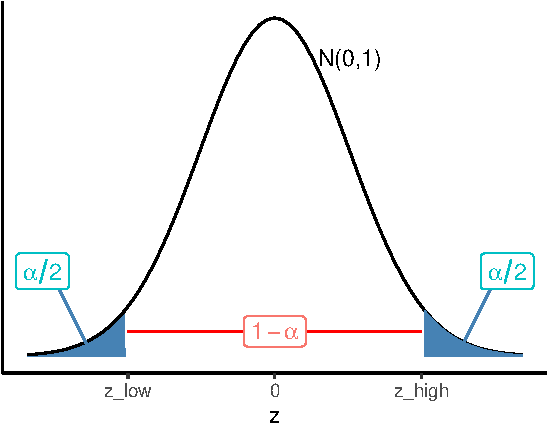
\includegraphics[keepaspectratio]{math340-notes_files/figure-latex/alpha-over-2-tails-1.pdf}}
\caption{\label{fig:alpha-over-2-tails}Finding z scores used to build a 2-sided confidence interval with desired confidence level}
\end{figure}

Similarly, a level \((1-\alpha)\) \textbf{lower bound for \(\theta\)} is \[\hat{\theta} - z_{\alpha}\cdot \sigma_{\hat{\theta}}\] (which defines the lower one-sided confidence interval \([\hat{\theta} - z_{\alpha}\cdot \sigma_{\hat{\theta}},\infty)\)) (see Figure \ref{fig:lower-one-sided-CI}).

A level \((1-\alpha)\) \textbf{upper bound for \(\theta\)} is \[\hat{\theta} + z_{\alpha}\cdot \sigma_{\hat{\theta}}\] (which defines the upper one-sided confidence interval \((-\infty,\hat{\theta}+z_{\alpha}\cdot \sigma_{\hat{\theta}}]\)) (see Figure \ref{fig:upper-one-sided-CI}). Note

\begin{itemize}
\tightlist
\item
  \(z_\alpha =\) \texttt{qnorm}\((\alpha)\)
\end{itemize}

\begin{figure}
\centering
\pandocbounded{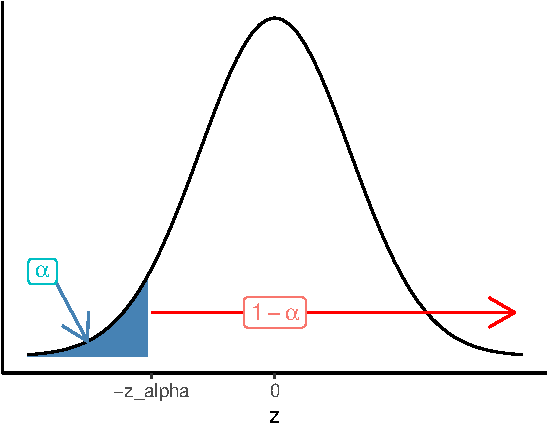
\includegraphics[keepaspectratio]{math340-notes_files/figure-latex/lower-one-sided-CI-1.pdf}}
\caption{\label{fig:lower-one-sided-CI}z scores corrsponding to lower 1-sided confidence interval}
\end{figure}

\begin{figure}
\centering
\pandocbounded{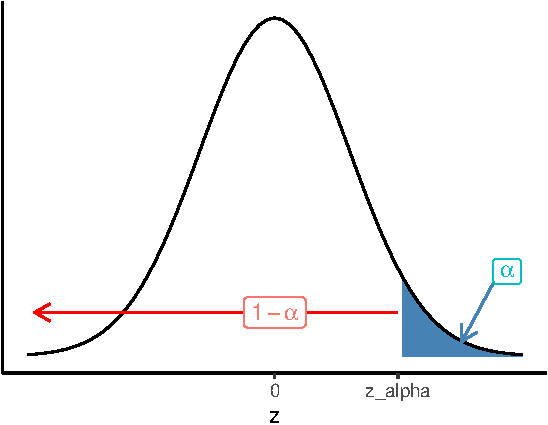
\includegraphics[keepaspectratio]{math340-notes_files/figure-latex/upper-one-sided-CI-1.pdf}}
\caption{\label{fig:upper-one-sided-CI}z scores corrsponding to upper 1-sided confidence interval}
\end{figure}

The scene outlined above applies to many situations, thanks to the Central Limit Theorem, including the four common scenarios mention in Chapter \ref{estimation}:

\begin{itemize}
\tightlist
\item
  1 mean \(\mu,\) estimated with sample mean \(\overline{X},\)
\item
  1 proportion \(p,\) estimate with sample proportion \(\hat{p},\)
\item
  difference of two means \(\mu_1-\mu_2,\) estimated with \(\overline{X_1}-\overline{X_2},\)
\item
  difference of two proportions \(p_1-p_2,\) estimated with \(\hat{p_1}-\hat{p_2}\).
\end{itemize}

We summarize these confidence intervals here:

\textbf{Common level \((1-\alpha)\) confidence intervals}

\begin{quote}
\begin{enumerate}
\def\labelenumi{\arabic{enumi}.}
\tightlist
\item
  For \(\mu\): \[\overline{X} \pm z_{\alpha/2} \cdot  \frac{\sigma}{\sqrt{n}}\]
\item
  For \(p\): \[\hat{p} \pm z_{\alpha/2} \sqrt{\frac{p(1-p)}{n}}\]
\item
  For \(\mu_1-\mu_2\): \[\left(\overline{X_1}-\overline{X_2}\right)\pm z_{\alpha/2} \frac{\sigma_1^2}{n_1} + \frac{\sigma_2^2}{n_2}\]
\item
  For \(p_1-p_2\): \[\left(\hat{p}_1-\hat{p}_2\right)\pm z_{\alpha/2} \sqrt{\frac{p_1(1-p_1)}{n_1}+\frac{p_2(1-p_2)}{n_2}}\]
\end{enumerate}
\end{quote}

For large sample sizes (\(n\geq 30\) is often sufficient), \(S\) can be used for unknown \(\sigma\) in confidence intervals for means, and sample proportions \(\hat{p}\) can be used for unknown \(p\).
For small sample sizes, when \(\sigma\) is unknown, we shall use \(T = \frac{\overline{X}-\mu}{S/\sqrt{n}}\) when estimating means, and we have the following confidence interval for \(\mu\):

\begin{quote}
For small sample sizes, when \(\sigma\) is unknown, we estimate \(\mu\) with \[\displaystyle \overline{X} \pm t_{\alpha/2} \cdot  \frac{S}{\sqrt{n}}\]
\end{quote}

Let's work through several examples.

\begin{example}
Suppose we gather a sample of size \(n = 20\) from a \(N(\mu,2)\) population, and find \(\overline{x} = 16.3\). Find a 98\% confidence interval for \(\mu\).

Here 98\% confidence \(\leftrightarrow \alpha = 0.02,\) and \(z_{\alpha/2} = z_{.01}\) = \texttt{qnorm(.99)} = 2.326.

So our 98\% confidence interval for the population mean \(\mu\) is \[\overline{x} \pm 2.326 \cdot \frac{2}{\sqrt{20}},\]
or \[16.3 \pm 1.04,\] or \[15.26 \text{ to } 17.34.\]
\end{example}

\begin{example}
Suppose in this example we don't know \(\sigma = 2,\) but in our sample of size 20 from \(N(\mu,\sigma),\) \(\overline{x} = 16.3\) and \(s = 2.13\). Find a 98\% confidence interval for \(\mu\).

Using a sample standard deviation \(s\) in place of \(\sigma\) requires us to use \(t\) instead of \(z\). In particular, instead of using \(z_{.01} = 2.326,\) we must use \(t_{.01}(19),\) the value in the t(19) distribution that has 1\% of the distribution greater than it.

So \(t_{.01}(19)\) = \texttt{qt(.99,19)} = 2.539. (This t-score will always be larger than the corresponding z-score, making the confidence interval wider than it would have been if we knew \(\sigma\).

Our confidence interval looks like:
\[\overline{x} \pm 2.539 \cdot \frac{2.13}{\sqrt{20}},\]
which simplifies to \[16.3 \pm 1.21,\] or, equivalently \[15.09 \text{ to } 17.51.\]
\end{example}

\begin{example}
In a poll of 500 likely voters, 260 say they support a particular local measure. Based on this sample, find a 90\% confidence interval for \(p,\) the proportion of all likely voters in favor of this measure.

We use the large sample confidence interval for \(p\). From the data, \(n = 500,\) \(\hat{p} = 260/500 = .52,\) and for 90\% confidence \(\alpha = 0.1,\) so \[z_{\alpha/2} = z_{.05} = 1.645,\]
(computed in R with \texttt{qnorm(.95)}). Now evaluate:

\begin{align*}
\hat{p} \pm z_{\alpha/2} \sqrt{\frac{\hat{p}(1-\hat{p})}{n}} &= .52 \pm 1.645 \sqrt{\frac{(.52)(.48)}{500}}\\
&= .52 \pm .037\\
&= .483 \text{ to } .557.
\end{align*}

It looks like it will be a close vote! We do not have convincing evidence, really, that \(p > .5\) since .5 lands inside the interval.
\end{example}

\begin{example}[Angles of spider webs]
The \href{https://www.google.com/books/edition/A_Handbook_of_Small_Data_Sets/vWu-MJM_obsC?hl=en}{Handbook of Small Data Sets} published in 1994 has lots of interesting, small data sets. Here's one small data set:

\begin{Shaded}
\begin{Highlighting}[]
\NormalTok{X }\OtherTok{=} \FunctionTok{c}\NormalTok{(}\DecValTok{25}\NormalTok{,}\DecValTok{12}\NormalTok{,}\DecValTok{31}\NormalTok{,}\DecValTok{26}\NormalTok{,}\DecValTok{17}\NormalTok{,}\DecValTok{15}\NormalTok{,}\DecValTok{24}\NormalTok{,}\DecValTok{10}\NormalTok{,}\DecValTok{16}\NormalTok{,}\DecValTok{12}\NormalTok{)}
\end{Highlighting}
\end{Shaded}

Spider webs' angles made with the vertical to the earth's surface have a \href{https://en.wikipedia.org/wiki/Von_Mises_distribution}{von Mises circular distribution} with known mean direction, \(\mu,\) and \(\mu\) varies from species to species. For instance,

\begin{itemize}
\tightlist
\item
  \emph{Isoxya cicatricosa} has \(\mu = 28.12^\circ,\) while
\item
  \emph{Araneus rufipalpus} has \(\mu = 15.66^\circ,\) obviously.
\end{itemize}

The question arose (in the article ``Sequential analysis for angular data'', by Gadsden and Kanji, (1981), \emph{The Statistician}, \textbf{30}, 119-129) of which species had constructed the 10 webs whose angles were listed above in the vector \texttt{X}.

Treating the data as a simple random sample we can construct a 95\% confidence interval for \(\mu\). Since the sample size is small, we use \(t_{\alpha/2},\) rather than \(z_{\alpha/2},\) where, here \(\alpha = .05\). Let's crunch out the interval in R.

\begin{Shaded}
\begin{Highlighting}[]
\CommentTok{\#summary statistics}
\NormalTok{n }\OtherTok{=} \FunctionTok{length}\NormalTok{(X)}
\NormalTok{xbar }\OtherTok{=} \FunctionTok{mean}\NormalTok{(X)}
\NormalTok{s }\OtherTok{=} \FunctionTok{sd}\NormalTok{(X)}
\NormalTok{tstar }\OtherTok{=} \FunctionTok{qt}\NormalTok{(.}\DecValTok{975}\NormalTok{,}\DecValTok{9}\NormalTok{) }\CommentTok{\#we let tstar denote t\_\{alpha/2\}}
\NormalTok{xbar }\SpecialCharTok{+} \FunctionTok{c}\NormalTok{(}\SpecialCharTok{{-}}\DecValTok{1}\NormalTok{,}\DecValTok{1}\NormalTok{)}\SpecialCharTok{*}\NormalTok{tstar}\SpecialCharTok{*}\NormalTok{s}\SpecialCharTok{/}\FunctionTok{sqrt}\NormalTok{(n)}
\end{Highlighting}
\end{Shaded}

\begin{verbatim}
## [1] 13.67688 23.92312
\end{verbatim}

Based on the interval, which contains the known mean for \emph{Araneus rufipalpus}, but not the known mean \emph{Isoxya cicatricosa}, we have good evidence that these webs were made by the former type of spider.
\end{example}

\begin{example}[Annual Snowfall in Buffalo, NY]

Here's another data set from the Handbook of Small Data Sets: The annual snowfall in Buffalo, NY (in inches) for the 63 years from 1910 to 1972.

\begin{verbatim}
##   year  snow
## 1 1910 126.4
## 2 1911  82.4
## 3 1912  78.1
## 4 1913  51.1
## 5 1914  90.9
\end{verbatim}

Let's find a 95\% confidence interval for the mean annual snowfall in Buffalo, taking the above snowfall column as a simple random sample of annual snowfall. Here are the summary statistics:

\begin{Shaded}
\begin{Highlighting}[]
\NormalTok{X }\OtherTok{=}\NormalTok{ snowfall}\SpecialCharTok{$}\NormalTok{snow }\CommentTok{\#snow fall column as vector X}
\NormalTok{n }\OtherTok{=} \FunctionTok{length}\NormalTok{(X)}
\NormalTok{xbar }\OtherTok{=} \FunctionTok{mean}\NormalTok{(X)}
\NormalTok{s }\OtherTok{=} \FunctionTok{sd}\NormalTok{(X)}
\end{Highlighting}
\end{Shaded}

For 95\% confidence, \(\alpha = .05,\) and \(z_{\alpha/2} = z_{.025} \approx 1.96.\)

Since \(n\) is large, we use the confidence interval formula below with \(s\) plugged in for \(\sigma\):

\[\overline{x} \pm z_{\alpha/2} \cdot  \frac{\sigma}{\sqrt{n}}\]
and we arrive at the interval

\begin{Shaded}
\begin{Highlighting}[]
\NormalTok{xbar }\SpecialCharTok{+} \FunctionTok{c}\NormalTok{(}\DecValTok{1}\NormalTok{,}\SpecialCharTok{{-}}\DecValTok{1}\NormalTok{)}\SpecialCharTok{*}\FunctionTok{qnorm}\NormalTok{(.}\DecValTok{025}\NormalTok{)}\SpecialCharTok{*}\NormalTok{s}\SpecialCharTok{/}\FunctionTok{sqrt}\NormalTok{(n)}
\end{Highlighting}
\end{Shaded}

\begin{verbatim}
## [1] 74.43965 86.15400
\end{verbatim}

\end{example}

\subsection*{\texorpdfstring{Confidence Intervals for \(\mu_1-\mu_2\)}{Confidence Intervals for \textbackslash mu\_1-\textbackslash mu\_2}}\label{confidence-intervals-for-mu_1-mu_2}
\addcontentsline{toc}{subsection}{Confidence Intervals for \(\mu_1-\mu_2\)}

Suppose we have two samples from two populations:
-an independent sample from population 1 which yields \(n_1,\) \(\overline{x}_1,\) \(s_1,\) and
-an independent sample from population 1 which yields \(n_2,\) \(\overline{x}_2,\) \(s_2\).
Moreover, the two samples are independent.

Recall, if Population 1 is \(N(\mu_1,\sigma_1)\) and Population 2 is \(N(\mu_2,\sigma_2\)), then a 95\% confidence interval for \(\mu_1-\mu_2\) is
\[\left(\overline{X_1}-\overline{X_2}\right)\pm z_{\alpha/2} \frac{\sigma_1^2}{n_1} + \frac{\sigma_2^2}{n_2}.\]
If \(\sigma_1\) and \(\sigma_2\) are unknown, but \(n_1\) and \(n_2\) are fairly large, it is reasonable to replace \(\sigma_1\) and \(\sigma_2\) with \(s_1\) and \(s_2,\) respectively.

If \(n_1, n_2\) are small (\(\leq 30\)) it's better to use a t-distribution.

Let's consider the special case that \(\sigma_1\) and \(\sigma_2\) are unknown but equal. Letting \(\sigma^2\) denote this common value. In this case we consider the pooled sample variance:
\[s_p^2 = \frac{(n_1-1)s_1^2 + (n_2-1)s_2^2}{n_1+n_2-2}\] as our (best) estimate of \(\sigma^2\). Then our level \((1-\alpha)\) confidence interval for \(\mu_1-\mu_2\) is \[\left(\overline{X_1}-\overline{X_2}\right)\pm t_{\alpha/2}S_p \sqrt{\frac{1}{n_1} + \frac{1}{n_2}},\]
where \(t_{\alpha/2}\) live in a t-distribution with \(n_1+n_2-2\) degrees of freedom.

\begin{example}
The silver content (\% Ag) of a number of Byzantine coins discovered in Cyprus was determined. Nine of the coins came from the first coinage of the reign of King Manuel, I, Comnenus (1143-1180); and 7 of the coins came from a coinage many years later.

\textbf{The data}

\begin{Shaded}
\begin{Highlighting}[]
\NormalTok{Ag1 }\OtherTok{\textless{}{-}} \FunctionTok{c}\NormalTok{(}\FloatTok{5.9}\NormalTok{,}\FloatTok{6.8}\NormalTok{,}\FloatTok{6.4}\NormalTok{,}\FloatTok{7.0}\NormalTok{,}\FloatTok{6.6}\NormalTok{,}\FloatTok{7.7}\NormalTok{,}\FloatTok{7.2}\NormalTok{,}\FloatTok{6.9}\NormalTok{,}\FloatTok{6.2}\NormalTok{)}
\NormalTok{Ag2 }\OtherTok{\textless{}{-}} \FunctionTok{c}\NormalTok{(}\FloatTok{5.3}\NormalTok{,}\FloatTok{5.6}\NormalTok{,}\FloatTok{5.5}\NormalTok{,}\FloatTok{5.1}\NormalTok{,}\FloatTok{6.2}\NormalTok{,}\FloatTok{5.8}\NormalTok{,}\FloatTok{5.8}\NormalTok{) }
\end{Highlighting}
\end{Shaded}

These data appear in \emph{The Handbook of Small Data Sets} (p.~118), and are based on this article:

Hendy, M.F. and Charles J.A. (1970), \emph{The production techniques, silver content and circulation history of the twelfth-century Byzantine Trachy.} Archaeonetry, 12. 13-21)

\textbf{The question}

Is there a significant difference in the silver content of coins minted early and late in Manuel's reign?

Let's conduct a small sample confidence interval for the difference in the two population means \(\mu_1 - \mu_2\) from the summary statistics:

\begin{table}[!h]
\centering
\begin{tabular}[t]{r|r|r|r}
\hline
sample & n & xbar & s\\
\hline
1 & 9 & 6.74 & 0.543\\
\hline
2 & 7 & 5.61 & 0.363\\
\hline
\end{tabular}
\end{table}

The pooled sample standard deviation is then \[s_p = \sqrt{\frac{8\cdot s_1^2 + 6 \cdot s_2^2}{14}} \approx .474,\]
and for 95\% confidence we use \(t^*\) = \texttt{qt(.975,14)} = 2.145. With all these values we have the following 95\% confidence interval for \(\mu_1 = \mu_2\): \[0.62 \text{ to } 1.64.\]
The entire interval lies above 0, so we have good evidence here of a difference between \(\mu_1\) and \(\mu_2\).
\end{example}

Was it reasonable in the previous example to assume the two populations have equal variance? Might differences in silver content in these two eras make it likely that other production differences existed as well (that might make variation in silver content from coin to coin also change)?

If \(\sigma_1^2\) and \(\sigma_2^2\) are unknown, sample sizes are samll, and its unreasonalbe to assume \(\sigma_1^2\) and \(\sigma_2^2\) are equal, one often sees the following (approximate) level \((1-\alpha)\) confidence interval for \(\mu_1 - \mu_2\):
\[\overline{X}_1 - \overline{X}_2 \pm t_{\alpha/2} \cdot \sqrt{\frac{s_1^2}{n_1}+\frac{s_2^2}{n_2}}\] where \(t_{\alpha/2}\) lives in a t-distribution with degrees of freedom equal to the minimum of \(n_1 - 1\) and \(n_2 - 1\).
So for the coin example, we would use \(t^*\) = \texttt{qt(.975,6)} = 2.447, giving us a wider confidence interval in the end:
\[0.574 \text{ to } 1.686,\] but still one that suggests a difference between \(\mu_1\) and \(\mu_2\).

\begin{example}[Recent Buffalo Snowfall]
With climate change, it may be unreasonable to assume the average annual snowfall now is the same as it was 100 years ago.

Let \(\mu_1\) denote the ``old'' mean average annual snowfall (and we assume the data from 1910 to 1972 is a random sample from the ``old'' population''), and \(\mu_2\) denots the ``new'' mean average annual snowfall in Buffalo (from which the annual snowfall from 2000 to 2021, found at \href{https://www.buffalo.org/snow}{buffalo.or/snow}, is a random sample.) Do these data provide evidence that \(\mu_1 \neq \mu_2\)?

Here are the 2001-2022 data:

\begin{Shaded}
\begin{Highlighting}[]
\NormalTok{Y }\OtherTok{=} \FunctionTok{c}\NormalTok{(}\FloatTok{158.7}\NormalTok{,}\FloatTok{132.4}\NormalTok{,}\FloatTok{111.3}\NormalTok{,}\FloatTok{100.9}\NormalTok{,}\FloatTok{109.1}\NormalTok{,}\FloatTok{78.2}\NormalTok{,}\FloatTok{88.9}\NormalTok{,}\FloatTok{103.8}\NormalTok{,}\FloatTok{100.2}\NormalTok{,}\FloatTok{74.1}\NormalTok{,}\FloatTok{111.8}\NormalTok{,}
      \FloatTok{36.7}\NormalTok{,}\FloatTok{58.8}\NormalTok{,}\FloatTok{129.9}\NormalTok{,}\FloatTok{112.9}\NormalTok{,}\FloatTok{55.1}\NormalTok{,}\FloatTok{76.1}\NormalTok{,}\FloatTok{112.3}\NormalTok{,}\FloatTok{118.8}\NormalTok{,}\FloatTok{69.2}\NormalTok{,}\FloatTok{77.2}\NormalTok{,}\FloatTok{97.4}\NormalTok{)}
\end{Highlighting}
\end{Shaded}

A 95\% confidence interval for the difference \(\mu_X-\mu_Y\):

TODO
\end{example}

\begin{example}[A one-sided confidence interval]
The measures of the outside diameter \(x_i\) (in inches) for 9 grains of the same type:

\begin{Shaded}
\begin{Highlighting}[]
\NormalTok{diam }\OtherTok{=} \FunctionTok{c}\NormalTok{(}\FloatTok{2.021}\NormalTok{,}\FloatTok{2.002}\NormalTok{,}\FloatTok{2.001}\NormalTok{,}\FloatTok{2.005}\NormalTok{,}\FloatTok{1.990}\NormalTok{,}\FloatTok{1.990}\NormalTok{,}\FloatTok{2.009}\NormalTok{,}\FloatTok{1.983}\NormalTok{,}\FloatTok{1.987}\NormalTok{)}
\end{Highlighting}
\end{Shaded}

Assume the distribution is normal. Is \(\mu \geq 2\)?

Let's find a 1-sided lower bound 95\% confidence interval for \(\mu,\) and see what that gets us.

Since \(n = 9\) is small and \(\sigma\) is unknown, we use the t-distribution.

Summary statistics:

\begin{itemize}
\tightlist
\item
  \(n = 9,\)
\item
  \(\overline{x}\) = \texttt{mean(diam)} = 1.9987.
\item
  \(s\) = \texttt{sd(diam)} = 0.0122
\end{itemize}

For a lower bound 95\% confidence interval, \(\alpha=.05\) and we use \[t_{\alpha} = t_{.05}(8) = qt(.95,8) = 1.86,\]
and the lower 1-sided interval is

\begin{align*}
(\overline{x}-t_{.05}(8)\cdot \frac{s}{\sqrt{n}},\infty) &= (1.9987 - 1.86\cdot\frac{0.0122}{\sqrt{9}},\infty) \\
&= (1.991,\infty)
\end{align*}

This confidence interval does not convince me that \(\mu \geq 2\).
(If the interval had been something like \([2.01,\infty),\) then I would be more convinced since we're confident that \(\mu\) is within the confidence interval, but with the interval \([1.991,\infty),\) best we can say is we're confident \(\mu \geq 1.99\).
\end{example}

\appendix


In MATH 340 we use R, a programming language designed for statistical analysis. In this tutorial we use R to estimate probability via simulation (repeated sampling from some set). We begin with data vectors, the structures we use to define sets in R.

\chapter{Sampling in R}\label{sampling-in-R}

\section{Data vectors}\label{vectors-R}

Use the \texttt{c()} command to enter an ordered list of elements. Separate entries with commas. The resulting object in R is called a \textbf{data vector}\index{R!vector}, or \textbf{vector}.

\subsection*{vector types}\label{vector-types}
\addcontentsline{toc}{subsection}{vector types}

We see vectors of three types: \textbf{numeric}, \textbf{character}, and \textbf{logical}.

A character vector consists of a list of strings. Strings are entered with quotes.

\begin{Shaded}
\begin{Highlighting}[]
\NormalTok{animals }\OtherTok{=} \FunctionTok{c}\NormalTok{(}\StringTok{"cat"}\NormalTok{,}\StringTok{"rabbit"}\NormalTok{,}\StringTok{"horse"}\NormalTok{,}\StringTok{"boar"}\NormalTok{,}\StringTok{"lynx"}\NormalTok{)}
\end{Highlighting}
\end{Shaded}

The vector \texttt{x} below is numeric. No quotes, just numbers.

\begin{Shaded}
\begin{Highlighting}[]
\NormalTok{x }\OtherTok{=} \FunctionTok{c}\NormalTok{(}\FloatTok{79.3}\NormalTok{,}\FloatTok{51.1}\NormalTok{,}\FloatTok{93.6}\NormalTok{,}\FloatTok{62.3}\NormalTok{,}\FloatTok{61.8}\NormalTok{)}
\end{Highlighting}
\end{Shaded}

A \textbf{logical} vector consists of a list of \texttt{TRUE}or \texttt{FALSE} elements (all caps!):

\begin{Shaded}
\begin{Highlighting}[]
\NormalTok{L }\OtherTok{=} \FunctionTok{c}\NormalTok{(}\ConstantTok{TRUE}\NormalTok{,}\ConstantTok{FALSE}\NormalTok{,}\ConstantTok{FALSE}\NormalTok{,}\ConstantTok{FALSE}\NormalTok{,}\ConstantTok{FALSE}\NormalTok{)}
\end{Highlighting}
\end{Shaded}

We can check the vector type with the \texttt{typeof()} command:

\begin{Shaded}
\begin{Highlighting}[]
\FunctionTok{typeof}\NormalTok{(animals)}
\end{Highlighting}
\end{Shaded}

\begin{verbatim}
## [1] "character"
\end{verbatim}

If you mix numbers and strings in a vector, R treats it as a character vector:

\begin{Shaded}
\begin{Highlighting}[]
\FunctionTok{typeof}\NormalTok{(}\FunctionTok{c}\NormalTok{(}\DecValTok{1}\NormalTok{,}\DecValTok{2}\NormalTok{,}\StringTok{"potato"}\NormalTok{))}
\end{Highlighting}
\end{Shaded}

\begin{verbatim}
## [1] "character"
\end{verbatim}

We may wish to place data vectors into a two-dimensional structure such as a matrix or a data frame.

\subsection*{matrices}\label{matrices}
\addcontentsline{toc}{subsection}{matrices}

Create a matrix from a vector with the \texttt{matrix()}\index{R!matrix} command, specifying how many rows, and whether we enter the data in the matrix by row, or by column.

\begin{Shaded}
\begin{Highlighting}[]
\FunctionTok{matrix}\NormalTok{(}\FunctionTok{c}\NormalTok{(}\StringTok{"a"}\NormalTok{,}\StringTok{"a"}\NormalTok{,}\StringTok{"a"}\NormalTok{,}\StringTok{"b"}\NormalTok{,}\StringTok{"b"}\NormalTok{,}\StringTok{"b"}\NormalTok{,}\StringTok{"c"}\NormalTok{,}\StringTok{"c"}\NormalTok{,}\StringTok{"c"}\NormalTok{,}\StringTok{"d"}\NormalTok{,}\StringTok{"d"}\NormalTok{,}\StringTok{"d"}\NormalTok{),}\AttributeTok{nrow =} \DecValTok{4}\NormalTok{,}\AttributeTok{byrow=}\ConstantTok{TRUE}\NormalTok{)}
\end{Highlighting}
\end{Shaded}

\begin{verbatim}
##      [,1] [,2] [,3]
## [1,] "a"  "a"  "a" 
## [2,] "b"  "b"  "b" 
## [3,] "c"  "c"  "c" 
## [4,] "d"  "d"  "d"
\end{verbatim}

\begin{Shaded}
\begin{Highlighting}[]
\FunctionTok{matrix}\NormalTok{(}\FunctionTok{c}\NormalTok{(}\StringTok{"a"}\NormalTok{,}\StringTok{"a"}\NormalTok{,}\StringTok{"a"}\NormalTok{,}\StringTok{"b"}\NormalTok{,}\StringTok{"b"}\NormalTok{,}\StringTok{"b"}\NormalTok{,}\StringTok{"c"}\NormalTok{,}\StringTok{"c"}\NormalTok{,}\StringTok{"c"}\NormalTok{,}\StringTok{"d"}\NormalTok{,}\StringTok{"d"}\NormalTok{,}\StringTok{"d"}\NormalTok{),}\AttributeTok{nrow =} \DecValTok{3}\NormalTok{,}\AttributeTok{byrow=}\ConstantTok{FALSE}\NormalTok{)}
\end{Highlighting}
\end{Shaded}

\begin{verbatim}
##      [,1] [,2] [,3] [,4]
## [1,] "a"  "b"  "c"  "d" 
## [2,] "a"  "b"  "c"  "d" 
## [3,] "a"  "b"  "c"  "d"
\end{verbatim}

\subsection*{data frames}\label{data-frames}
\addcontentsline{toc}{subsection}{data frames}

A data frame links related vectors as columns in an array via the \texttt{data.frame()}\index{R!data frame} command.

\begin{Shaded}
\begin{Highlighting}[]
\NormalTok{a }\OtherTok{=} \FunctionTok{c}\NormalTok{(}\StringTok{"McMinnville"}\NormalTok{,}\StringTok{"Denver"}\NormalTok{,}\StringTok{"Minneapolis"}\NormalTok{,}\StringTok{"Charleston"}\NormalTok{)}
\NormalTok{x }\OtherTok{=} \FunctionTok{c}\NormalTok{(}\FloatTok{45.21}\NormalTok{,}\FloatTok{39.74}\NormalTok{,}\FloatTok{44.98}\NormalTok{,}\FloatTok{32.78}\NormalTok{)}
\NormalTok{y }\OtherTok{=} \FunctionTok{c}\NormalTok{(}\FloatTok{123.19}\NormalTok{,}\FloatTok{104.99}\NormalTok{,}\FloatTok{93.26}\NormalTok{,}\FloatTok{79.93}\NormalTok{)}
\NormalTok{df }\OtherTok{=} \FunctionTok{data.frame}\NormalTok{(}\AttributeTok{city =}\NormalTok{ a, }\AttributeTok{latitude =}\NormalTok{ x, }\AttributeTok{longitude =}\NormalTok{ y)}
\NormalTok{df}
\end{Highlighting}
\end{Shaded}

\begin{verbatim}
##          city latitude longitude
## 1 McMinnville    45.21    123.19
## 2      Denver    39.74    104.99
## 3 Minneapolis    44.98     93.26
## 4  Charleston    32.78     79.93
\end{verbatim}

Data frames are a common way to manage related data vectors in R.

\subsection*{common vector commands}\label{common-vector-commands}
\addcontentsline{toc}{subsection}{common vector commands}

Here's a vector of Hank Aaron's home run totals in each of his seasons in Major League Baseball:

\begin{Shaded}
\begin{Highlighting}[]
\NormalTok{hr }\OtherTok{=} \FunctionTok{c}\NormalTok{(}\DecValTok{13}\NormalTok{,}\DecValTok{27}\NormalTok{,}\DecValTok{26}\NormalTok{,}\DecValTok{44}\NormalTok{,}\DecValTok{30}\NormalTok{,}\DecValTok{39}\NormalTok{,}\DecValTok{40}\NormalTok{,}\DecValTok{34}\NormalTok{,}\DecValTok{45}\NormalTok{,}\DecValTok{44}\NormalTok{,}\DecValTok{24}\NormalTok{,}\DecValTok{32}\NormalTok{,}\DecValTok{44}\NormalTok{,}\DecValTok{39}\NormalTok{,}\DecValTok{29}\NormalTok{,}\DecValTok{44}\NormalTok{,}\DecValTok{38}\NormalTok{,}\DecValTok{47}\NormalTok{,}\DecValTok{34}\NormalTok{,}\DecValTok{40}\NormalTok{,}\DecValTok{20}\NormalTok{,}\DecValTok{12}\NormalTok{,}\DecValTok{10}\NormalTok{)}
\end{Highlighting}
\end{Shaded}

With \texttt{hr} loaded into your session, you can refer to it by name when you want to extract features of it. Here are some commonly used commands on numeric vectors:

\begin{itemize}
\tightlist
\item
  \texttt{length(hr)}, number of elements in the vector (number of seasons Hank played)
\item
  \texttt{sum(hr)}, the sum of the vector (total career home runs)
\item
  \texttt{mean(hr)}, the mean of the vector (average HR per season)
\item
  \texttt{max(hr)}, the max (best HR total in a season)
\item
  \texttt{sd(hr)}, standard deviation
\item
  \texttt{diff(hr)} returns a vector whose elements are the differences between consecutive elements in the vector \texttt{hr}
\item
  \texttt{cumsum(hr)} returns a vector whose elements are the cumulative sum of the vector \texttt{hr}
\item
  \texttt{rev(hr)} returns the vector in the reverse order
\end{itemize}

Behold:

\begin{Shaded}
\begin{Highlighting}[]
\FunctionTok{diff}\NormalTok{(hr)}
\end{Highlighting}
\end{Shaded}

\begin{verbatim}
##  [1]  14  -1  18 -14   9   1  -6  11  -1 -20   8  12  -5 -10  15  -6   9 -13   6
## [20] -20  -8  -2
\end{verbatim}

\begin{Shaded}
\begin{Highlighting}[]
\FunctionTok{cumsum}\NormalTok{(hr)}
\end{Highlighting}
\end{Shaded}

\begin{verbatim}
##  [1]  13  40  66 110 140 179 219 253 298 342 366 398 442 481 510 554 592 639 673
## [20] 713 733 745 755
\end{verbatim}

\subsection*{comparison operators}\label{comparison-operators}
\addcontentsline{toc}{subsection}{comparison operators}

We use \emph{comparison operators} to compare things in R and return a value of \texttt{TRUE} or \texttt{FALSE}:

\begin{itemize}
\tightlist
\item
  equal to \texttt{==}
\item
  not equal to \texttt{!=}
\item
  less than \texttt{\textless{}}
\item
  less than or equal to \texttt{\textless{}=}
\item
  greater than \texttt{\textgreater{}}
\item
  greater than or equal to \texttt{\textgreater{}=}
\end{itemize}

A few examples:

\begin{Shaded}
\begin{Highlighting}[]
\DecValTok{12} \SpecialCharTok{\textgreater{}=} \DecValTok{5}
\end{Highlighting}
\end{Shaded}

\begin{verbatim}
## [1] TRUE
\end{verbatim}

Use \textbf{double equal signs} \texttt{==} to see whether two things are equal:

\begin{Shaded}
\begin{Highlighting}[]
\DecValTok{16} \SpecialCharTok{==} \DecValTok{2}\SpecialCharTok{*}\DecValTok{8}
\end{Highlighting}
\end{Shaded}

\begin{verbatim}
## [1] TRUE
\end{verbatim}

\begin{Shaded}
\begin{Highlighting}[]
\StringTok{"ab"}\SpecialCharTok{==}\StringTok{"ba"}
\end{Highlighting}
\end{Shaded}

\begin{verbatim}
## [1] FALSE
\end{verbatim}

\begin{Shaded}
\begin{Highlighting}[]
\NormalTok{x }\OtherTok{=} \DecValTok{3} \CommentTok{\# this defines the variable}
\NormalTok{x}\SpecialCharTok{\^{}}\DecValTok{2}\SpecialCharTok{+}\DecValTok{3}\SpecialCharTok{*}\NormalTok{x }\SpecialCharTok{==} \DecValTok{12} \CommentTok{\#this asks whether x\^{}2 + 3*x equals 12 for the currently stored value of x (x=3 in this case)}
\end{Highlighting}
\end{Shaded}

\begin{verbatim}
## [1] FALSE
\end{verbatim}

Logical vectors arise when we give R a proposition involving a vector:

\begin{Shaded}
\begin{Highlighting}[]
\FunctionTok{c}\NormalTok{(}\DecValTok{1}\NormalTok{,}\DecValTok{8}\NormalTok{,}\DecValTok{4}\NormalTok{,}\DecValTok{6}\NormalTok{) }\SpecialCharTok{\textgreater{}} \DecValTok{5}
\end{Highlighting}
\end{Shaded}

\begin{verbatim}
## [1] FALSE  TRUE FALSE  TRUE
\end{verbatim}

\subsection*{checking membership}\label{checking-membership}
\addcontentsline{toc}{subsection}{checking membership}

The \texttt{\%in\%} command can be used to ask whether a particular element is contained in a vector.

\begin{Shaded}
\begin{Highlighting}[]
\NormalTok{v }\OtherTok{=} \FunctionTok{c}\NormalTok{(}\StringTok{"bob"}\NormalTok{,}\StringTok{"wilma"}\NormalTok{,}\StringTok{"hedgie"}\NormalTok{)}
\StringTok{"frank"} \SpecialCharTok{\%in\%}\NormalTok{ v}
\end{Highlighting}
\end{Shaded}

\begin{verbatim}
## [1] FALSE
\end{verbatim}

\begin{Shaded}
\begin{Highlighting}[]
\StringTok{"wilma"} \SpecialCharTok{\%in\%}\NormalTok{ v}
\end{Highlighting}
\end{Shaded}

\begin{verbatim}
## [1] TRUE
\end{verbatim}

\subsection*{\texorpdfstring{\texttt{sum()} and \texttt{which()}}{sum() and which()}}\label{sum-and-which}
\addcontentsline{toc}{subsection}{\texttt{sum()} and \texttt{which()}}

The \texttt{sum()} command on a numeric vector adds the elements of the vector, as we saw above with \texttt{sum(hr)}.

The \texttt{sum()} command on a logical vector returns the number of TRUE elements in the vector.

\begin{Shaded}
\begin{Highlighting}[]
\FunctionTok{sum}\NormalTok{(}\FunctionTok{c}\NormalTok{(}\ConstantTok{TRUE}\NormalTok{,}\ConstantTok{FALSE}\NormalTok{,}\ConstantTok{TRUE}\NormalTok{,}\ConstantTok{FALSE}\NormalTok{,}\ConstantTok{TRUE}\NormalTok{,}\ConstantTok{TRUE}\NormalTok{))}
\end{Highlighting}
\end{Shaded}

\begin{verbatim}
## [1] 4
\end{verbatim}

We can thus easily count the number of elements in a vector meeting some condition:

\begin{Shaded}
\begin{Highlighting}[]
\FunctionTok{sum}\NormalTok{(hr }\SpecialCharTok{\textgreater{}=} \DecValTok{40}\NormalTok{)}
\end{Highlighting}
\end{Shaded}

\begin{verbatim}
## [1] 8
\end{verbatim}

8 seasons with at least 40 HR?!! Of course! 8! Ok, which seasons?

\begin{Shaded}
\begin{Highlighting}[]
\FunctionTok{which}\NormalTok{(hr }\SpecialCharTok{\textgreater{}=} \DecValTok{40}\NormalTok{)}
\end{Highlighting}
\end{Shaded}

\begin{verbatim}
## [1]  4  7  9 10 13 16 18 20
\end{verbatim}

The \texttt{which()} command returns the indices of the vector at which the condition being tested has been met. So Hank hit 40 or more HR in seasons 4, 7, 9, 10, 13, 16, 18, and 20.

\subsection*{extracting elements}\label{extracting-elements}
\addcontentsline{toc}{subsection}{extracting elements}

Recall Hank Aaron's home runs by season:

\begin{Shaded}
\begin{Highlighting}[]
\NormalTok{hr}
\end{Highlighting}
\end{Shaded}

\begin{verbatim}
##  [1] 13 27 26 44 30 39 40 34 45 44 24 32 44 39 29 44 38 47 34 40 20 12 10
\end{verbatim}

We can \textbf{extract an element} of a vector by indicating its {[}position{]}:

\begin{Shaded}
\begin{Highlighting}[]
\NormalTok{hr[}\DecValTok{3}\NormalTok{]}
\end{Highlighting}
\end{Shaded}

\begin{verbatim}
## [1] 26
\end{verbatim}

Or we can specify several elements:

\begin{Shaded}
\begin{Highlighting}[]
\NormalTok{hr[}\FunctionTok{c}\NormalTok{(}\DecValTok{1}\NormalTok{,}\DecValTok{3}\NormalTok{,}\DecValTok{5}\NormalTok{)]}
\end{Highlighting}
\end{Shaded}

\begin{verbatim}
## [1] 13 26 30
\end{verbatim}

\subsection*{comparing vectors}\label{comparing-vectors}
\addcontentsline{toc}{subsection}{comparing vectors}

We can count the number of positions in which two vectors of the same length agree

\begin{Shaded}
\begin{Highlighting}[]
\NormalTok{v }\OtherTok{=} \FunctionTok{c}\NormalTok{(}\DecValTok{3}\NormalTok{,}\DecValTok{2}\NormalTok{,}\DecValTok{6}\NormalTok{,}\DecValTok{8}\NormalTok{); w }\OtherTok{=} \FunctionTok{c}\NormalTok{(}\DecValTok{2}\NormalTok{,}\DecValTok{3}\NormalTok{,}\DecValTok{1}\NormalTok{,}\DecValTok{8}\NormalTok{)}
\FunctionTok{sum}\NormalTok{(v}\SpecialCharTok{==}\NormalTok{w) }\CommentTok{\# how often they match}
\end{Highlighting}
\end{Shaded}

\begin{verbatim}
## [1] 1
\end{verbatim}

We can find the position(s) at which they agree

\begin{Shaded}
\begin{Highlighting}[]
\FunctionTok{which}\NormalTok{(v}\SpecialCharTok{==}\NormalTok{w) }\CommentTok{\#where they match}
\end{Highlighting}
\end{Shaded}

\begin{verbatim}
## [1] 4
\end{verbatim}

and list the matching value(s):

\begin{Shaded}
\begin{Highlighting}[]
\NormalTok{v[}\FunctionTok{which}\NormalTok{(v}\SpecialCharTok{==}\NormalTok{w)] }
\end{Highlighting}
\end{Shaded}

\begin{verbatim}
## [1] 8
\end{verbatim}

\subsection*{vector arithmetic}\label{vector-arithmetic}
\addcontentsline{toc}{subsection}{vector arithmetic}

We can do element-wise arithmetic on two vectors of equal length, such as addition, subtraction, multiplication, division, and exponentiation.

\begin{Shaded}
\begin{Highlighting}[]
\NormalTok{v }\OtherTok{=} \FunctionTok{c}\NormalTok{(}\SpecialCharTok{{-}}\DecValTok{1}\NormalTok{,}\DecValTok{1}\NormalTok{,}\DecValTok{3}\NormalTok{)}
\NormalTok{w }\OtherTok{=} \FunctionTok{c}\NormalTok{(}\DecValTok{1}\NormalTok{,}\DecValTok{4}\NormalTok{,}\DecValTok{5}\NormalTok{)}
\end{Highlighting}
\end{Shaded}

\begin{longtable}[]{@{}lll@{}}
\toprule\noalign{}
Operation & Result & \\
\midrule\noalign{}
\endhead
\bottomrule\noalign{}
\endlastfoot
\texttt{v\ +\ w} & 0, 5, 8 & \\
\texttt{v\ -\ w} & -2, -3, -2 & \\
\texttt{v\ *\ w} & -1, 4, 15 & \\
\texttt{v\ /\ w} & -1, 0.25, 0.6 & \\
\texttt{v\^{}w} & -1, 1, 243 & \\
\end{longtable}

We also have scalar multiplication,

\begin{Shaded}
\begin{Highlighting}[]
\DecValTok{8}\SpecialCharTok{*}\NormalTok{v}
\end{Highlighting}
\end{Shaded}

\begin{verbatim}
## [1] -8  8 24
\end{verbatim}

and you can add a scalar to each element in a vector:

\begin{Shaded}
\begin{Highlighting}[]
\DecValTok{8} \SpecialCharTok{+}\NormalTok{ v}
\end{Highlighting}
\end{Shaded}

\begin{verbatim}
## [1]  7  9 11
\end{verbatim}

\subsection*{concatenate vectors}\label{concatenate-vectors}
\addcontentsline{toc}{subsection}{concatenate vectors}

The \texttt{c()} command allows you to concatenate vectors:

\begin{Shaded}
\begin{Highlighting}[]
\NormalTok{u }\OtherTok{=} \FunctionTok{c}\NormalTok{(}\DecValTok{1}\NormalTok{,}\DecValTok{2}\NormalTok{,}\DecValTok{3}\NormalTok{)}
\NormalTok{v }\OtherTok{=} \FunctionTok{c}\NormalTok{(}\DecValTok{4}\NormalTok{,}\DecValTok{5}\NormalTok{,}\DecValTok{6}\NormalTok{)}
\FunctionTok{c}\NormalTok{(u,v)}
\end{Highlighting}
\end{Shaded}

\begin{verbatim}
## [1] 1 2 3 4 5 6
\end{verbatim}

We can add an element to a vector \texttt{A} via concatenation:

\begin{Shaded}
\begin{Highlighting}[]
\NormalTok{A }\OtherTok{=} \FunctionTok{c}\NormalTok{(}\StringTok{"Will"}\NormalTok{,}\StringTok{"Lucas"}\NormalTok{,}\StringTok{"Mike"}\NormalTok{,}\StringTok{"Dustin"}\NormalTok{)}
\NormalTok{A }\OtherTok{=} \FunctionTok{c}\NormalTok{(A,}\StringTok{"Eleven"}\NormalTok{)}
\NormalTok{A}
\end{Highlighting}
\end{Shaded}

\begin{verbatim}
## [1] "Will"   "Lucas"  "Mike"   "Dustin" "Eleven"
\end{verbatim}

Notice, the vector \texttt{A} currently has 5 elements. We can add a 6th element can also to \texttt{A} directly:

\begin{Shaded}
\begin{Highlighting}[]
\NormalTok{A[}\DecValTok{6}\NormalTok{]}\OtherTok{=}\StringTok{"Max"} \CommentTok{\# creates new position after the last previous position}
\NormalTok{A}
\end{Highlighting}
\end{Shaded}

\begin{verbatim}
## [1] "Will"   "Lucas"  "Mike"   "Dustin" "Eleven" "Max"
\end{verbatim}

\section{Special vectors}\label{special-vectors}

\subsection*{consecutive integers}\label{consecutive-integers}
\addcontentsline{toc}{subsection}{consecutive integers}

\textbf{The integers 1 to n} can be entered by typing \texttt{1:n}. For instance, we could define a 20 sided die by entering

\begin{Shaded}
\begin{Highlighting}[]
\NormalTok{die }\OtherTok{=} \DecValTok{1}\SpecialCharTok{:}\DecValTok{20}
\end{Highlighting}
\end{Shaded}

More generally, entering \texttt{a:b} creates a vector of consecutive integers starting with \texttt{a} and ending with \texttt{b} (even if \texttt{a} is greater than or equal to \texttt{b}).

\begin{Shaded}
\begin{Highlighting}[]
\DecValTok{8}\SpecialCharTok{:}\DecValTok{2}
\end{Highlighting}
\end{Shaded}

\begin{verbatim}
## [1] 8 7 6 5 4 3 2
\end{verbatim}

\subsection*{letters}\label{letters}
\addcontentsline{toc}{subsection}{letters}

\begin{Shaded}
\begin{Highlighting}[]
\NormalTok{letters}
\end{Highlighting}
\end{Shaded}

\begin{verbatim}
##  [1] "a" "b" "c" "d" "e" "f" "g" "h" "i" "j" "k" "l" "m" "n" "o" "p" "q" "r" "s"
## [20] "t" "u" "v" "w" "x" "y" "z"
\end{verbatim}

Want the set of capital letters?

\begin{Shaded}
\begin{Highlighting}[]
\NormalTok{LETTERS}
\end{Highlighting}
\end{Shaded}

\begin{verbatim}
##  [1] "A" "B" "C" "D" "E" "F" "G" "H" "I" "J" "K" "L" "M" "N" "O" "P" "Q" "R" "S"
## [20] "T" "U" "V" "W" "X" "Y" "Z"
\end{verbatim}

\subsection*{\texorpdfstring{\texttt{rep()}}{rep()}}\label{rep}
\addcontentsline{toc}{subsection}{\texttt{rep()}}

The \texttt{rep()} command lets us build a vector with lots of repeated elements.

\begin{example}
\protect\hypertarget{exm:skittles}{}\label{exm:skittles}

Let's say we want to create a \textbf{bag of skittles} with this color distribution: 40 red, 30 orange, 25 yellow, 60 green, and 20 purple.

The \texttt{rep()} command let's us do this quickly. One approach:
- first enter the distinct items (as a vector with the \texttt{c()} command!),
- then enter how many times each occurs (as a vector!):

\begin{Shaded}
\begin{Highlighting}[]
\NormalTok{skittles }\OtherTok{=} \FunctionTok{rep}\NormalTok{(}\FunctionTok{c}\NormalTok{(}\StringTok{"red"}\NormalTok{,}\StringTok{"orange"}\NormalTok{,}\StringTok{"yellow"}\NormalTok{,}\StringTok{"green"}\NormalTok{,}\StringTok{"purple"}\NormalTok{),}
               \FunctionTok{c}\NormalTok{(}\DecValTok{40}\NormalTok{,}\DecValTok{30}\NormalTok{,}\DecValTok{25}\NormalTok{,}\DecValTok{60}\NormalTok{,}\DecValTok{20}\NormalTok{)}
\NormalTok{               )}
\end{Highlighting}
\end{Shaded}

One can also construct this bag of skittles by running

\begin{Shaded}
\begin{Highlighting}[]
\NormalTok{skittles }\OtherTok{=} \FunctionTok{c}\NormalTok{(}\FunctionTok{rep}\NormalTok{(}\StringTok{\textquotesingle{}red\textquotesingle{}}\NormalTok{, }\DecValTok{40}\NormalTok{),}
             \FunctionTok{rep}\NormalTok{(}\StringTok{\textquotesingle{}orange\textquotesingle{}}\NormalTok{, }\DecValTok{30}\NormalTok{),}
             \FunctionTok{rep}\NormalTok{(}\StringTok{\textquotesingle{}yellow\textquotesingle{}}\NormalTok{, }\DecValTok{25}\NormalTok{),}
             \FunctionTok{rep}\NormalTok{(}\StringTok{\textquotesingle{}green\textquotesingle{}}\NormalTok{, }\DecValTok{60}\NormalTok{),}
             \FunctionTok{rep}\NormalTok{(}\StringTok{\textquotesingle{}purple\textquotesingle{}}\NormalTok{, }\DecValTok{20}\NormalTok{))}
\end{Highlighting}
\end{Shaded}

\end{example}

\subsection*{\texorpdfstring{\texttt{table()}}{table()}}\label{table}
\addcontentsline{toc}{subsection}{\texttt{table()}}

The \texttt{table()} command is a handy way to see which unique values are contained in a vector and how often each unique value occurs. In otherwords, \texttt{table(v)} gives the frequency distribution for a vector \texttt{v}:

\begin{Shaded}
\begin{Highlighting}[]
\FunctionTok{table}\NormalTok{(skittles)}
\end{Highlighting}
\end{Shaded}

\begin{verbatim}
## skittles
##  green orange purple    red yellow 
##     60     30     20     40     25
\end{verbatim}

\subsection*{\texorpdfstring{\texttt{seq()}}{seq()}}\label{seq}
\addcontentsline{toc}{subsection}{\texttt{seq()}}

The \texttt{seq()} command lets us enter an \emph{arithmetic progression} by entering (first, last, increment).

A few examples

\begin{Shaded}
\begin{Highlighting}[]
\FunctionTok{seq}\NormalTok{(}\DecValTok{0}\NormalTok{, }\DecValTok{1}\NormalTok{, }\AttributeTok{by=}\NormalTok{.}\DecValTok{1}\NormalTok{)}
\end{Highlighting}
\end{Shaded}

\begin{verbatim}
##  [1] 0.0 0.1 0.2 0.3 0.4 0.5 0.6 0.7 0.8 0.9 1.0
\end{verbatim}

\begin{Shaded}
\begin{Highlighting}[]
\FunctionTok{seq}\NormalTok{(}\DecValTok{0}\NormalTok{, }\DecValTok{100}\NormalTok{, }\AttributeTok{by =} \DecValTok{10}\NormalTok{)}
\end{Highlighting}
\end{Shaded}

\begin{verbatim}
##  [1]   0  10  20  30  40  50  60  70  80  90 100
\end{verbatim}

Ok, now let's get to \textbf{sampling}!

\section{Sampling}\label{sampling-in-R-section}

We use the \texttt{sample(x,...)} command to sample from vector \texttt{x}.

For instance, we can draw a random sample of size 2 from a vector of colors:

\begin{Shaded}
\begin{Highlighting}[]
\NormalTok{x }\OtherTok{=} \FunctionTok{c}\NormalTok{(}\StringTok{\textquotesingle{}red\textquotesingle{}}\NormalTok{,}\StringTok{\textquotesingle{}pink\textquotesingle{}}\NormalTok{,}\StringTok{\textquotesingle{}orange\textquotesingle{}}\NormalTok{,}\StringTok{\textquotesingle{}green\textquotesingle{}}\NormalTok{,}\StringTok{\textquotesingle{}yellow\textquotesingle{}}\NormalTok{,}\StringTok{\textquotesingle{}purple\textquotesingle{}}\NormalTok{)}
\FunctionTok{sample}\NormalTok{(x,}\DecValTok{2}\NormalTok{)}
\end{Highlighting}
\end{Shaded}

\begin{verbatim}
## [1] "green"  "purple"
\end{verbatim}

Here's another example. Let's grab 20 skittles at random from the bag \texttt{skittles} we created in Example \ref{exm:skittles} and count how many orange ones we get:

\begin{Shaded}
\begin{Highlighting}[]
\NormalTok{grab}\OtherTok{=}\FunctionTok{sample}\NormalTok{(skittles,}\DecValTok{20}\NormalTok{)}
\FunctionTok{table}\NormalTok{(grab)}
\end{Highlighting}
\end{Shaded}

\begin{verbatim}
## grab
##  green orange purple    red yellow 
##      9      4      1      5      1
\end{verbatim}

The \texttt{table()} command counts how many of each color :), which is more than we asked for. We could have found the orange count directly with

\begin{Shaded}
\begin{Highlighting}[]
\FunctionTok{sum}\NormalTok{(grab}\SpecialCharTok{==}\StringTok{"orange"}\NormalTok{)}
\end{Highlighting}
\end{Shaded}

\begin{verbatim}
## [1] 4
\end{verbatim}

\subsection*{\texorpdfstring{\texttt{sample()} options}{sample() options}}\label{sample-options}
\addcontentsline{toc}{subsection}{\texttt{sample()} options}

Typically, we provide the \texttt{sample()} command with 3 or 4 arguments, in this order:

\begin{itemize}
\tightlist
\item
  \texttt{x}, the vector we sample from
\item
  \texttt{size}, the size of the sample
\item
  \texttt{replace}, whether you sample with or without replacement (default = FALSE)
\item
  \texttt{prob}, custom probabilities for the sampling of elements (default = equal probability for all elements in \texttt{x})
\end{itemize}

If you enter your arguments in the order \texttt{x=,\ size=,\ replace=,\ prob=} then you do not need to specify the variable names.

If you do not specify their value, the \texttt{sample()} command assumes the following \textbf{default values}:

\begin{itemize}
\tightlist
\item
  \texttt{size} = the length of the vector
\item
  \texttt{replace} = FALSE
\item
  \texttt{prob} is set so all elements in the vector have equal probability of being chosen.
\end{itemize}

Here are handy special cases, illustrated with this vector:

\begin{Shaded}
\begin{Highlighting}[]
\NormalTok{animals }\OtherTok{=} \FunctionTok{c}\NormalTok{(}\StringTok{"cat"}\NormalTok{,}\StringTok{"dog"}\NormalTok{,}\StringTok{"hedgehog"}\NormalTok{,}\StringTok{"rabbit"}\NormalTok{)}
\end{Highlighting}
\end{Shaded}

\subsubsection*{permutations}\label{permutations-1}
\addcontentsline{toc}{subsubsection}{permutations}

Use \texttt{sample(x)} to generate a \emph{random permutation} of \texttt{x}:

\begin{Shaded}
\begin{Highlighting}[]
\FunctionTok{sample}\NormalTok{(animals) }\CommentTok{\#default size is the length of the vector}
\end{Highlighting}
\end{Shaded}

\begin{verbatim}
## [1] "dog"      "rabbit"   "hedgehog" "cat"
\end{verbatim}

\subsubsection*{repeated sampling of one element}\label{repeated-sampling-of-one-element}
\addcontentsline{toc}{subsubsection}{repeated sampling of one element}

Use \texttt{sample()} to simulate picking one element of \texttt{animals} \(n\) times by setting \texttt{size\ =\ n} and \texttt{replace\ =\ TRUE}.

Example: Draw one animal from the set 1000 different times and summarize the picks with a table.

\begin{Shaded}
\begin{Highlighting}[]
\NormalTok{picks }\OtherTok{=} \FunctionTok{sample}\NormalTok{(animals, }\DecValTok{1000}\NormalTok{, }\AttributeTok{replace =} \ConstantTok{TRUE}\NormalTok{) }
\FunctionTok{table}\NormalTok{(picks) }
\end{Highlighting}
\end{Shaded}

\begin{verbatim}
## picks
##      cat      dog hedgehog   rabbit 
##      263      233      231      273
\end{verbatim}

And the winner is\ldots{} rabbit!

Or, since we fear rabbits and love dogs, we can do repeated sampling of a single element with \textbf{custom probabilities}:

\begin{Shaded}
\begin{Highlighting}[]
\NormalTok{picks2 }\OtherTok{=} \FunctionTok{sample}\NormalTok{(animals,}
                \AttributeTok{size=}\DecValTok{1000}\NormalTok{,}
                \AttributeTok{replace=}\ConstantTok{TRUE}\NormalTok{,}
                \AttributeTok{prob=}\FunctionTok{c}\NormalTok{(.}\DecValTok{2}\NormalTok{, .}\DecValTok{4}\NormalTok{, .}\DecValTok{3}\NormalTok{, .}\DecValTok{1}\NormalTok{))}
\FunctionTok{table}\NormalTok{(picks2)}
\end{Highlighting}
\end{Shaded}

\begin{verbatim}
## picks2
##      cat      dog hedgehog   rabbit 
##      202      369      317      112
\end{verbatim}

Nice!

Remember, the default option for \texttt{sample()} is to sample without replacement, and with equal probabilities.

\subsection*{sample without replacement}\label{sample-without-replacement}
\addcontentsline{toc}{subsection}{sample without replacement}

\begin{quote}
\textbf{Task}:
Pick 4 students at random from a class of 9 to race around Taylor Hall. (Assumes we have numbered the students 1-9).
\end{quote}

\begin{Shaded}
\begin{Highlighting}[]
\FunctionTok{sample}\NormalTok{(}\DecValTok{1}\SpecialCharTok{:}\DecValTok{9}\NormalTok{,}\DecValTok{4}\NormalTok{)}
\end{Highlighting}
\end{Shaded}

\begin{verbatim}
## [1] 8 7 1 4
\end{verbatim}

\subsection*{sample with replacement}\label{sample-with-replacement}
\addcontentsline{toc}{subsection}{sample with replacement}

\begin{quote}
\textbf{Task}:
On twelve consecutive days, ask one student at random, in a class of size 9, to write a solution on the board.
\end{quote}

\begin{Shaded}
\begin{Highlighting}[]
\FunctionTok{sample}\NormalTok{(}\DecValTok{1}\SpecialCharTok{:}\DecValTok{9}\NormalTok{,}\DecValTok{12}\NormalTok{,}\AttributeTok{replace=}\ConstantTok{TRUE}\NormalTok{)}
\end{Highlighting}
\end{Shaded}

\begin{verbatim}
##  [1] 9 2 4 6 8 3 3 9 7 3 9 5
\end{verbatim}

\subsection*{sample with custom probabilities}\label{sample-with-custom-probabilities}
\addcontentsline{toc}{subsection}{sample with custom probabilities}

\begin{quote}
\textbf{Task}:
Roll a weighted 6 sided die with the following probability distribution 100 times and summarize the results.
\end{quote}

\begin{longtable}[]{@{}lllllll@{}}
\toprule\noalign{}
\(x\) & 1 & 2 & 3 & 4 & 5 & 6 \\
\midrule\noalign{}
\endhead
\bottomrule\noalign{}
\endlastfoot
\(p(x)\) & .2 & .1 & .05 & .4 & .1 & .15 \\
\end{longtable}

\begin{Shaded}
\begin{Highlighting}[]
\NormalTok{rolls }\OtherTok{=} \FunctionTok{sample}\NormalTok{(}\DecValTok{1}\SpecialCharTok{:}\DecValTok{6}\NormalTok{,}
               \AttributeTok{size=}\DecValTok{100}\NormalTok{,}
               \AttributeTok{replace=}\ConstantTok{TRUE}\NormalTok{,}
               \AttributeTok{prob=}\FunctionTok{c}\NormalTok{(.}\DecValTok{2}\NormalTok{, .}\DecValTok{1}\NormalTok{, .}\DecValTok{05}\NormalTok{, .}\DecValTok{4}\NormalTok{, .}\DecValTok{1}\NormalTok{, .}\DecValTok{15}\NormalTok{))}
\FunctionTok{table}\NormalTok{(rolls)}
\end{Highlighting}
\end{Shaded}

\begin{verbatim}
## rolls
##  1  2  3  4  5  6 
## 22  8  4 45  6 15
\end{verbatim}

\subsection*{example: lefties}\label{example-lefties}
\addcontentsline{toc}{subsection}{example: lefties}

\begin{quote}
\textbf{Task}:
8\% of a population is left-handed. Draw a random sample of 45 people from the population and record the number of lefties.
\end{quote}

One approach: build a large population with these features and then draw 45 people from it without replacement.

\begin{Shaded}
\begin{Highlighting}[]
\NormalTok{pop}\OtherTok{=}\FunctionTok{rep}\NormalTok{(}\FunctionTok{c}\NormalTok{(}\StringTok{"L"}\NormalTok{,}\StringTok{"R"}\NormalTok{),}\FunctionTok{c}\NormalTok{(}\DecValTok{800}\NormalTok{,}\DecValTok{9200}\NormalTok{)) }\CommentTok{\# a population of 10,000 people, 800 of them lefties}
\FunctionTok{table}\NormalTok{(}\FunctionTok{sample}\NormalTok{(pop,}\AttributeTok{size=}\DecValTok{45}\NormalTok{)) }
\end{Highlighting}
\end{Shaded}

\begin{verbatim}
## 
##  L  R 
##  4 41
\end{verbatim}

A second approach: sample with replacement 45 times from a ``two-sided'' die with customized probabilities

\begin{Shaded}
\begin{Highlighting}[]
\NormalTok{die}\OtherTok{=}\FunctionTok{c}\NormalTok{(}\StringTok{"L"}\NormalTok{,}\StringTok{"R"}\NormalTok{)}
\FunctionTok{table}\NormalTok{(}\FunctionTok{sample}\NormalTok{(die,}\AttributeTok{size=}\DecValTok{45}\NormalTok{,}\AttributeTok{replace=}\ConstantTok{TRUE}\NormalTok{,}\AttributeTok{prob=}\FunctionTok{c}\NormalTok{(.}\DecValTok{08}\NormalTok{,.}\DecValTok{92}\NormalTok{)))}
\end{Highlighting}
\end{Shaded}

\begin{verbatim}
## 
##  L  R 
##  2 43
\end{verbatim}

A third approach: Use a binomial distribution (later)

\section{Repeated sampling}\label{repeated-sampling}

Let's say we have a huge urn full of orange and blue marbles, and 42\% of them are orange. We can use repeated sampling to approximate the \textbf{sampling distribution} for the number of orange marbles we would draw in a sample of, say, 50 marbles.
The sampling distribution provides information about what sorts of orange marble counts should we expect, and how often should we expect these counts.

\emph{Repeated sampling} can estimate this sampling distribution. Here are two methods for achieving repeated sampling in R.

\subsection*{\texorpdfstring{using a \texttt{for} loop}{using a for loop}}\label{using-a-for-loop}
\addcontentsline{toc}{subsection}{using a \texttt{for} loop}

The code below creates a vector called \texttt{orange\_counts} that, eventually, after the for loop has completed, has 10000 entries. Each entry in this vector gives the number of orange marbles drawn from the urn from a random sample of 50 marbles.

\begin{Shaded}
\begin{Highlighting}[]
\NormalTok{colors}\OtherTok{=}\FunctionTok{c}\NormalTok{(}\StringTok{"orange"}\NormalTok{,}\StringTok{"blue"}\NormalTok{)}
\NormalTok{orange\_counts}\OtherTok{=}\FunctionTok{c}\NormalTok{() }\CommentTok{\#a vector for storing the results of each trial}
\ControlFlowTok{for}\NormalTok{ (i }\ControlFlowTok{in} \DecValTok{1}\SpecialCharTok{:}\DecValTok{10000}\NormalTok{)\{}
\NormalTok{  grab }\OtherTok{=} \FunctionTok{sample}\NormalTok{(colors, }\DecValTok{50}\NormalTok{, }\AttributeTok{replace =} \ConstantTok{TRUE}\NormalTok{, }\AttributeTok{prob =} \FunctionTok{c}\NormalTok{(.}\DecValTok{42}\NormalTok{, .}\DecValTok{58}\NormalTok{))}
\NormalTok{  orange\_counts[i]}\OtherTok{=}\FunctionTok{sum}\NormalTok{(grab }\SpecialCharTok{==} \StringTok{"orange"}\NormalTok{)}
\NormalTok{\}}
\end{Highlighting}
\end{Shaded}

We know that \texttt{table(orange\_counts)} displays the counts of each of the unique values occurring in \texttt{orange\_counts}. We can visualize these counts with a \texttt{barplot()}:

\begin{Shaded}
\begin{Highlighting}[]
\FunctionTok{barplot}\NormalTok{(}\FunctionTok{table}\NormalTok{(orange\_counts))}
\end{Highlighting}
\end{Shaded}

\pandocbounded{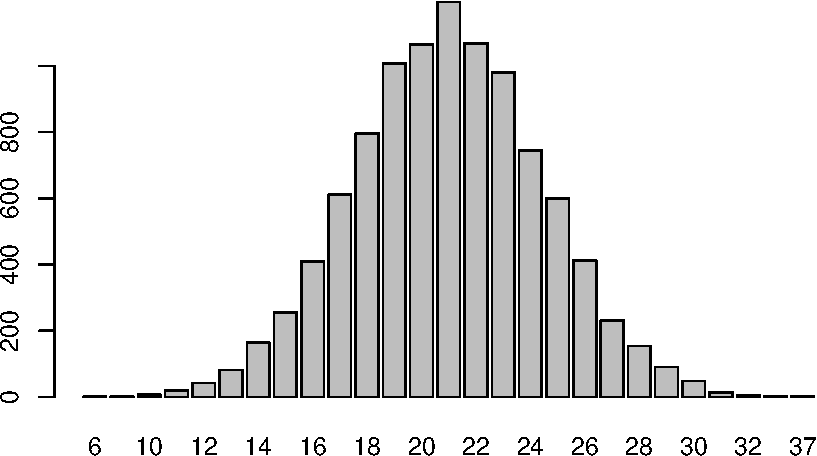
\includegraphics[keepaspectratio]{math340-notes_files/figure-latex/unnamed-chunk-101-1.pdf}}

\subsection*{\texorpdfstring{using \texttt{replicate()}}{using replicate()}}\label{using-replicate}
\addcontentsline{toc}{subsection}{using \texttt{replicate()}}

The \texttt{replicate()} command essentially does the above for loop for us :) The command \texttt{replicate(n,expr)}will evaluate \texttt{expr} \texttt{n} times, and store the results.

\begin{Shaded}
\begin{Highlighting}[]
\NormalTok{colors}\OtherTok{=}\FunctionTok{c}\NormalTok{(}\StringTok{"orange"}\NormalTok{,}\StringTok{"blue"}\NormalTok{)}
\NormalTok{orange\_counts }\OtherTok{=} 
  \FunctionTok{replicate}\NormalTok{(}\DecValTok{10000}\NormalTok{,}
            \FunctionTok{sum}\NormalTok{(}\FunctionTok{sample}\NormalTok{(colors, }\DecValTok{50}\NormalTok{, }\AttributeTok{replace=}\ConstantTok{TRUE}\NormalTok{, }\AttributeTok{prob=}\FunctionTok{c}\NormalTok{(.}\DecValTok{42}\NormalTok{, .}\DecValTok{58}\NormalTok{)) }\SpecialCharTok{==} \StringTok{"orange"}\NormalTok{)}
\NormalTok{            )}
\end{Highlighting}
\end{Shaded}

Again, we can summarize the \emph{frequency} with which each value of orange\_counts occurs with \texttt{table()}, and visualize this frequency table with a \texttt{barplot}:

\begin{Shaded}
\begin{Highlighting}[]
\FunctionTok{barplot}\NormalTok{(}\FunctionTok{table}\NormalTok{(orange\_counts))}
\end{Highlighting}
\end{Shaded}

\pandocbounded{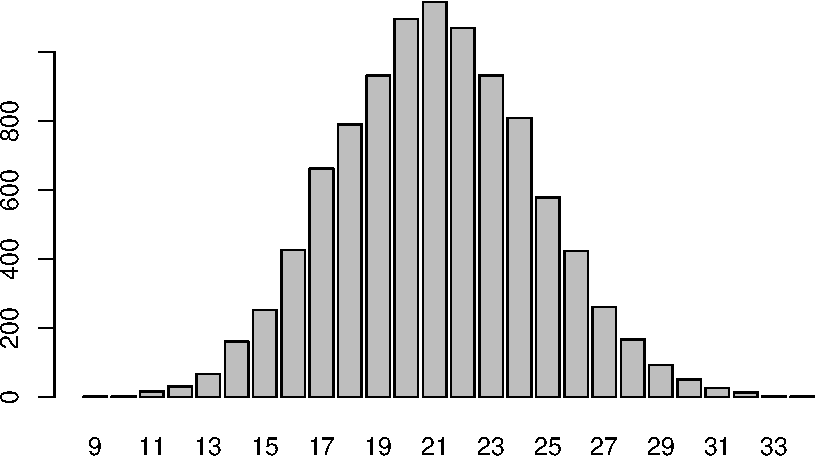
\includegraphics[keepaspectratio]{math340-notes_files/figure-latex/unnamed-chunk-103-1.pdf}}

In addition, we can calculate summary statistics to put numbers to qualitative descriptions of the distribution of values in \texttt{orange\_counts} such as center and spread. These statistics help us answer the question of what sorts of orange counts to expect.

\begin{longtable}[]{@{}lll@{}}
\toprule\noalign{}
statistic & command & result \\
\midrule\noalign{}
\endhead
\bottomrule\noalign{}
\endlastfoot
mean & \texttt{mean(orange\_counts)} & 21.0289 \\
standard deviation & \texttt{sd(orange\_counts)} & 3.4616561 \\
five number summary & \texttt{fivenum(orange\_counts)} & 8, 19, 21, 23, 36 \\
\end{longtable}

\section{Summary of R commands}\label{sampling-commands}

\subsection*{defining vectors}\label{defining-vectors}
\addcontentsline{toc}{subsection}{defining vectors}

\begin{longtable}[]{@{}
  >{\raggedright\arraybackslash}p{(\linewidth - 4\tabcolsep) * \real{0.0882}}
  >{\raggedright\arraybackslash}p{(\linewidth - 4\tabcolsep) * \real{0.3922}}
  >{\raggedright\arraybackslash}p{(\linewidth - 4\tabcolsep) * \real{0.5196}}@{}}
\toprule\noalign{}
\begin{minipage}[b]{\linewidth}\raggedright
Command
\end{minipage} & \begin{minipage}[b]{\linewidth}\raggedright
Description
\end{minipage} & \begin{minipage}[b]{\linewidth}\raggedright
Example
\end{minipage} \\
\midrule\noalign{}
\endhead
\bottomrule\noalign{}
\endlastfoot
\texttt{c()} & List the elements & \texttt{x\ =\ c("a","c","c","z","z","z")} \\
\texttt{a:b} & Consecutive integers from \texttt{a} to \texttt{b} & \texttt{8:4} returns the vector 8, 7, 6, 5, 4 \\
\texttt{rep()} & Build a vector from a frequency table & \texttt{rep(c("y","n"),c(3,2))} returns y, y, y, n, n \\
\texttt{seq()} & Arithmetic progression (first,last,step) & \texttt{seq(0,1,.2)} returns 0, 0.2, 0.4, 0.6, 0.8, 1 \\
\end{longtable}

\subsection*{summarizing vectors}\label{summarizing-vectors}
\addcontentsline{toc}{subsection}{summarizing vectors}

\begin{longtable}[]{@{}
  >{\raggedright\arraybackslash}p{(\linewidth - 2\tabcolsep) * \real{0.1250}}
  >{\raggedright\arraybackslash}p{(\linewidth - 2\tabcolsep) * \real{0.8750}}@{}}
\toprule\noalign{}
\begin{minipage}[b]{\linewidth}\raggedright
Command
\end{minipage} & \begin{minipage}[b]{\linewidth}\raggedright
Description
\end{minipage} \\
\midrule\noalign{}
\endhead
\bottomrule\noalign{}
\endlastfoot
\texttt{typeof(x)} & the vector type of \texttt{x} (usually \emph{character}, \emph{numeric}, or \emph{logical}) \\
\texttt{length(x)} & the length of \texttt{x} (how many elements it has) \\
\texttt{table(x)} & the frequency table (which values occur in \texttt{x} along with how often each value occurs) \\
\end{longtable}

\subsection*{sampling from vectors}\label{sampling-from-vectors}
\addcontentsline{toc}{subsection}{sampling from vectors}

\begin{longtable}[]{@{}
  >{\raggedright\arraybackslash}p{(\linewidth - 2\tabcolsep) * \real{0.4479}}
  >{\raggedright\arraybackslash}p{(\linewidth - 2\tabcolsep) * \real{0.5521}}@{}}
\toprule\noalign{}
\begin{minipage}[b]{\linewidth}\raggedright
Sampling Options
\end{minipage} & \begin{minipage}[b]{\linewidth}\raggedright
Example with \texttt{x\ =\ 1:6}
\end{minipage} \\
\midrule\noalign{}
\endhead
\bottomrule\noalign{}
\endlastfoot
permutation of \texttt{x} & \texttt{sample(x)\ =} 6, 3, 1, 5, 2, 4 \\
sample \(n\) elements without replacement & \texttt{sample(x,3)\ =} 5, 1, 3 \\
sample \(n\) elements with replacement & \texttt{sample(x,5,replace=T)\ =} 3, 3, 6, 4, 6 \\
sample with custom probabilities & \texttt{sample(x,10,replace=T,prob=\ c(0,.2,0,.5,.1,.2))\ =} 4, 5, 6, 4, 5, 4, 6, 6, 2, 6 \\
\end{longtable}

\chapter{Simulating Probability in R}\label{R-sim-probability}

We can use repeated sampling of a chance experiment to estimate the probability of some event. The examples here were chosen to provide an introduction to sampling scenarios that you may find useful in this class (rolling dice, flipping coins, drawing names from a hat, marbles from a box,\ldots). These examples also assume no previous knowledge of R beyond what was covered in Appendix \ref{sampling-in-R}, and have been ordered roughly by my view of the complexity of the coding involved.

\section{Difference of two dice}\label{diff-2dice-R}

\begin{quote}
If you roll 2 6-sided dice, what is the likelihood that their values are 1 apart.
\end{quote}

Our Strategy: roll the two dice, record the absolute value of their difference, repeat!

Code:

\begin{Shaded}
\begin{Highlighting}[]
\NormalTok{trials }\OtherTok{=} \DecValTok{10000}
\NormalTok{die\_1 }\OtherTok{=} \DecValTok{1}\SpecialCharTok{:}\DecValTok{6}
\NormalTok{die\_2 }\OtherTok{=} \DecValTok{1}\SpecialCharTok{:}\DecValTok{6}
\NormalTok{results }\OtherTok{=} \FunctionTok{c}\NormalTok{() }\CommentTok{\#will store the difference of the two dice each trial}
\ControlFlowTok{for}\NormalTok{ (i }\ControlFlowTok{in} \DecValTok{1}\SpecialCharTok{:}\NormalTok{trials)\{}
\NormalTok{  roll\_1 }\OtherTok{=} \FunctionTok{sample}\NormalTok{(die\_1, }\DecValTok{1}\NormalTok{)}
\NormalTok{  roll\_2 }\OtherTok{=} \FunctionTok{sample}\NormalTok{(die\_2, }\DecValTok{1}\NormalTok{)}
\NormalTok{  difference }\OtherTok{=} \FunctionTok{abs}\NormalTok{(roll\_1 }\SpecialCharTok{{-}}\NormalTok{ roll\_2) }\CommentTok{\#absolute value is abs()}
\NormalTok{  results[i] }\OtherTok{=}\NormalTok{ difference}
\NormalTok{\}}
\end{Highlighting}
\end{Shaded}

Results:

\begin{Shaded}
\begin{Highlighting}[]
\FunctionTok{table}\NormalTok{(results)}
\end{Highlighting}
\end{Shaded}

\begin{verbatim}
## results
##    0    1    2    3    4    5 
## 1646 2862 2196 1658 1119  519
\end{verbatim}

Conclusion: By computing the ratio \texttt{sum(results\ ==\ 1)\ /\ trials}, we obtain our estimate of the probability the two dice to be 1 apart:
0.2862.

Referring to the 6x6 grid recording the difference for each of the 36 possible outcomes in Table \ref{tab:diff-2-dice}, we would find the actual probability equal to 10/36 \(\approx\) 0.278.

\section{Oregon License Plates}\label{license-plates-R}

\begin{quote}
Classic Oregon license plates consist of 3 letters (A-Z) followed by 3 numbers (0-9). Find the probability that a randomly selected plate has two 8s.
\end{quote}

This is not such an interesting probability question - at least not one we need to simulate - but it's fun to build a random Oregon license plate!

Strategy:

\begin{enumerate}
\def\labelenumi{\arabic{enumi}.}
\tightlist
\item
  Build a random plate. We want three random capital letters (repeats ok), followed by three random numbers (repeats ok). So, we sample from \texttt{LETTERS} 3 times with replacement, then 0:9 three times with replacement.
\end{enumerate}

\begin{Shaded}
\begin{Highlighting}[]
\NormalTok{plate }\OtherTok{=} \FunctionTok{c}\NormalTok{(}\FunctionTok{sample}\NormalTok{(LETTERS, }\DecValTok{3}\NormalTok{, }\AttributeTok{replace =} \ConstantTok{TRUE}\NormalTok{),}
          \FunctionTok{sample}\NormalTok{(}\DecValTok{0}\SpecialCharTok{:}\DecValTok{9}\NormalTok{, }\DecValTok{3}\NormalTok{, }\AttributeTok{replace =} \ConstantTok{TRUE}\NormalTok{))}
\NormalTok{plate}
\end{Highlighting}
\end{Shaded}

\begin{verbatim}
## [1] "P" "X" "X" "7" "8" "2"
\end{verbatim}

Fun!

\begin{enumerate}
\def\labelenumi{\arabic{enumi}.}
\setcounter{enumi}{1}
\tightlist
\item
  Count how many ``8''s are in the plate
\end{enumerate}

\begin{Shaded}
\begin{Highlighting}[]
\FunctionTok{sum}\NormalTok{(plate }\SpecialCharTok{==} \StringTok{"8"}\NormalTok{)}
\end{Highlighting}
\end{Shaded}

\begin{verbatim}
## [1] 1
\end{verbatim}

\textbf{Final Code}

\begin{Shaded}
\begin{Highlighting}[]
\NormalTok{trials }\OtherTok{=} \DecValTok{10000}
\NormalTok{results }\OtherTok{=} \FunctionTok{c}\NormalTok{()}
\ControlFlowTok{for}\NormalTok{ (i }\ControlFlowTok{in} \DecValTok{1}\SpecialCharTok{:}\NormalTok{trials)\{}
\NormalTok{  plate }\OtherTok{=} \FunctionTok{c}\NormalTok{(}\FunctionTok{sample}\NormalTok{(LETTERS,}\DecValTok{3}\NormalTok{,}\AttributeTok{replace=}\ConstantTok{TRUE}\NormalTok{),}
            \FunctionTok{sample}\NormalTok{(}\DecValTok{0}\SpecialCharTok{:}\DecValTok{9}\NormalTok{,}\DecValTok{3}\NormalTok{,}\AttributeTok{replace=}\ConstantTok{TRUE}\NormalTok{)) }\CommentTok{\#build a plate}
\NormalTok{  eights }\OtherTok{=} \FunctionTok{sum}\NormalTok{(plate}\SpecialCharTok{==}\StringTok{"8"}\NormalTok{) }\CommentTok{\# count the 8s}
\NormalTok{  results }\OtherTok{=} \FunctionTok{c}\NormalTok{(results,eights) }\CommentTok{\# update the results vector}
\NormalTok{\}}
\FunctionTok{table}\NormalTok{(results)}
\end{Highlighting}
\end{Shaded}

\begin{verbatim}
## results
##    0    1    2    3 
## 7263 2468  258   11
\end{verbatim}

Based on this simulation, we estimate the probability of having a plate with exactly 2 ``8''s

\begin{Shaded}
\begin{Highlighting}[]
\FunctionTok{sum}\NormalTok{(results}\SpecialCharTok{==}\StringTok{"2"}\NormalTok{)}\SpecialCharTok{/}\NormalTok{trials}
\end{Highlighting}
\end{Shaded}

\begin{verbatim}
## [1] 0.0258
\end{verbatim}

Using our counting tools to calculate the probability (and we really don't need to keep track of the letters in the plate, but we do):

\[\frac{26\cdot 26\cdot 26 \cdot \binom{3}{2} \cdot 1 \cdot 1 \cdot 9}{26^3\cdot 10^3}= \frac{27}{1000} = 0.027.\]

\section{Rolling a 10-sided die}\label{10sided-die-R}

\begin{quote}
We're rolling a fair 10-sided die. Use simulation to estimate the probability that the first time we roll an 8 or higher is on the 5th roll.
\end{quote}

\textbf{Scratch Work}

\begin{enumerate}
\def\labelenumi{\arabic{enumi}.}
\tightlist
\item
  Simulate rolling a 10-sided die 5 times. (Sample 5 times with replacement from the vector 1:10.)
\end{enumerate}

\begin{Shaded}
\begin{Highlighting}[]
\NormalTok{die }\OtherTok{=} \DecValTok{1}\SpecialCharTok{:}\DecValTok{10}
\NormalTok{rolls }\OtherTok{=} \FunctionTok{sample}\NormalTok{(die, }\DecValTok{5}\NormalTok{, }\AttributeTok{replace =} \ConstantTok{TRUE}\NormalTok{)}
\end{Highlighting}
\end{Shaded}

\begin{enumerate}
\def\labelenumi{\arabic{enumi}.}
\setcounter{enumi}{1}
\tightlist
\item
  We want code to check whether a random sequence of 5 rolls has these five features: Rolls 1-4 are less than 8, and roll 5 is an 8, 9, or 10.
\end{enumerate}

We can ask these five questions in R and store the answers in a logical vector:

\begin{Shaded}
\begin{Highlighting}[]
\FunctionTok{c}\NormalTok{(rolls[}\DecValTok{1}\SpecialCharTok{:}\DecValTok{4}\NormalTok{] }\SpecialCharTok{\textless{}} \DecValTok{8}\NormalTok{, rolls[}\DecValTok{5}\NormalTok{] }\SpecialCharTok{\textgreater{}=} \DecValTok{8}\NormalTok{)}
\end{Highlighting}
\end{Shaded}

\begin{verbatim}
## [1]  TRUE FALSE  TRUE  TRUE  TRUE
\end{verbatim}

Recall, the \texttt{sum()} of a logical vector counts the number of TRUE values. We need the sum to be 5 to have the kind of sequence we want to count.

\begin{Shaded}
\begin{Highlighting}[]
\FunctionTok{sum}\NormalTok{(}\FunctionTok{c}\NormalTok{(rolls[}\DecValTok{1}\SpecialCharTok{:}\DecValTok{4}\NormalTok{] }\SpecialCharTok{\textless{}} \DecValTok{8}\NormalTok{, rolls[}\DecValTok{5}\NormalTok{] }\SpecialCharTok{\textgreater{}=} \DecValTok{8}\NormalTok{)) }\CommentTok{\#does this sum equal 5?}
\end{Highlighting}
\end{Shaded}

\begin{verbatim}
## [1] 4
\end{verbatim}

I think we're ready!!

\textbf{Final Code}

\begin{Shaded}
\begin{Highlighting}[]
\NormalTok{trials }\OtherTok{=} \DecValTok{10000}
\NormalTok{results }\OtherTok{=} \FunctionTok{c}\NormalTok{() }\CommentTok{\#stores how many dice "do the right thing" in each trial}

\NormalTok{die }\OtherTok{=} \DecValTok{1}\SpecialCharTok{:}\DecValTok{10}
\ControlFlowTok{for}\NormalTok{ (i }\ControlFlowTok{in} \DecValTok{1}\SpecialCharTok{:}\NormalTok{trials)\{}
\NormalTok{  rolls }\OtherTok{=} \FunctionTok{sample}\NormalTok{(die,}\DecValTok{5}\NormalTok{,}\AttributeTok{replace=}\ConstantTok{TRUE}\NormalTok{) }\CommentTok{\# roll the 10{-}sided die 5 times}
\NormalTok{  x}\OtherTok{=}\FunctionTok{sum}\NormalTok{(}\FunctionTok{c}\NormalTok{(rolls[}\DecValTok{1}\SpecialCharTok{:}\DecValTok{4}\NormalTok{]}\SpecialCharTok{\textless{}}\DecValTok{8}\NormalTok{,rolls[}\DecValTok{5}\NormalTok{]}\SpecialCharTok{\textgreater{}=}\DecValTok{8}\NormalTok{)) }\CommentTok{\#how many dice "do the right thing"}
\NormalTok{  results}\OtherTok{=}\FunctionTok{c}\NormalTok{(results,x) }\CommentTok{\# update the results vector}
\NormalTok{\}}
\end{Highlighting}
\end{Shaded}

The results of the simulation:

\begin{Shaded}
\begin{Highlighting}[]
\FunctionTok{table}\NormalTok{(results)}
\end{Highlighting}
\end{Shaded}

\begin{verbatim}
## results
##    0    1    2    3    4    5 
##   60  588 2021 3746 2886  699
\end{verbatim}

Based on our simulation, we estimate the probability in question by the ratio: \texttt{sum(results\ ==\ 5)\ /\ trials} = 0.0699.

This estimated probability is likely very close to what we calculate by our counting tools: \[\frac{7^4\cdot 3}{10^5} \approx .07203.\]

Final note: In this example we added to the \texttt{results} vector each iteration by concatenation (\texttt{results=c(results,x)}) rather than by specifying \texttt{results{[}i{]}=x} in each trial, as we did in the difference of two dice example. Either approach works.

\section{Marbles from an urn}\label{marbles-urn-R}

\begin{quote}
An urn contains 100 orange and 200 green marbles. If you draw 8 marbles from the urn at random (without replacement), how likely is it that more than 5 of them are orange?
\end{quote}

\begin{Shaded}
\begin{Highlighting}[]
\NormalTok{urn }\OtherTok{=} \FunctionTok{rep}\NormalTok{(}\FunctionTok{c}\NormalTok{(}\StringTok{"orange"}\NormalTok{,}\StringTok{"green"}\NormalTok{),}\FunctionTok{c}\NormalTok{(}\DecValTok{100}\NormalTok{,}\DecValTok{200}\NormalTok{))}
\NormalTok{trials }\OtherTok{=} \DecValTok{10000}
\NormalTok{results }\OtherTok{=} \FunctionTok{c}\NormalTok{()}
\ControlFlowTok{for}\NormalTok{ (i }\ControlFlowTok{in} \DecValTok{1}\SpecialCharTok{:}\NormalTok{trials)\{}
\NormalTok{  grab }\OtherTok{=} \FunctionTok{sample}\NormalTok{(urn, }\DecValTok{8}\NormalTok{, }\AttributeTok{replace =} \ConstantTok{FALSE}\NormalTok{)}
\NormalTok{  orange\_count }\OtherTok{=} \FunctionTok{sum}\NormalTok{(grab }\SpecialCharTok{==} \StringTok{"orange"}\NormalTok{)}
\NormalTok{  results[i] }\OtherTok{=}\NormalTok{ orange\_count}
\NormalTok{\}}
\FunctionTok{table}\NormalTok{(results)}
\end{Highlighting}
\end{Shaded}

\begin{verbatim}
## results
##    0    1    2    3    4    5    6    7 
##  362 1561 2799 2727 1703  662  155   31
\end{verbatim}

We can enter \texttt{sum(results\ \textgreater{}\ 5)} to see how often we grabbed more than 5 orange marbles in our sample of size 8, and \texttt{sum(results\ \textgreater{}\ 5)/trials} is a good estimate of the likelihood of this happening.

Conclusion: It appears we should expect the more than 5 orange marbles in our sample of 8 about 1.9\% of the time:

\begin{Shaded}
\begin{Highlighting}[]
\FunctionTok{sum}\NormalTok{(results }\SpecialCharTok{\textgreater{}} \DecValTok{5}\NormalTok{)}\SpecialCharTok{/}\NormalTok{trials}
\end{Highlighting}
\end{Shaded}

\begin{verbatim}
## [1] 0.0186
\end{verbatim}

This question is a classic ``good potatoes/bad potatoes'' problem, and by our counting techniques, we know the probability is \[\frac{\binom{100}{6}\cdot\binom{200}{2}}{\binom{300}{8}}+
\frac{\binom{100}{7}\cdot\binom{200}{1}}{\binom{300}{8}}+
\frac{\binom{100}{8}\cdot\binom{200}{0}}{\binom{300}{8}},\]
which we can evaluate in R as a check:

\begin{Shaded}
\begin{Highlighting}[]
\FunctionTok{sum}\NormalTok{(}\FunctionTok{choose}\NormalTok{(}\DecValTok{100}\NormalTok{,}\DecValTok{6}\SpecialCharTok{:}\DecValTok{8}\NormalTok{)}\SpecialCharTok{*}\FunctionTok{choose}\NormalTok{(}\DecValTok{200}\NormalTok{,}\DecValTok{8{-}6}\SpecialCharTok{:}\DecValTok{8}\NormalTok{)}\SpecialCharTok{/}\FunctionTok{choose}\NormalTok{(}\DecValTok{300}\NormalTok{,}\DecValTok{8}\NormalTok{))}
\end{Highlighting}
\end{Shaded}

\begin{verbatim}
## [1] 0.01830405
\end{verbatim}

\emph{Note}: After studying common named discrete probability distributions, we will see that R has a nice built-in command for doing these sorts of computations.

\section{Tracking runs of Heads in coin flips}\label{flip-coin-R}

\begin{quote}
If you flip a coin 20 times, how likely is it to have a run of at least 5 Heads in a row?
\end{quote}

One approach:

\begin{itemize}
\tightlist
\item
  Build a coin vector: \texttt{coin\ =\ c("H","T")}
\item
  Build a vector for recording the outcomes of twenty flips: \texttt{flips\ =\ sample(coin,\ size\ =\ 20,\ replace\ =\ TRUE)}
\item
  Record the longest run of Heads in the sequence.
\item
  Repeat many, many times.
\end{itemize}

The following code plays this `flip a coin 20 times and record the longest run of heads' game for 10000 trials.

\begin{Shaded}
\begin{Highlighting}[]
\NormalTok{coin }\OtherTok{=} \FunctionTok{c}\NormalTok{(}\StringTok{"Heads"}\NormalTok{,}\StringTok{"Tails"}\NormalTok{)}
\NormalTok{trials}\OtherTok{=}\DecValTok{10000}
\NormalTok{results}\OtherTok{=}\FunctionTok{c}\NormalTok{() }\CommentTok{\#stores longest run of Heads each trial}
\ControlFlowTok{for}\NormalTok{ (i }\ControlFlowTok{in} \DecValTok{1}\SpecialCharTok{:}\NormalTok{trials)\{}
\NormalTok{  flips }\OtherTok{=} \FunctionTok{sample}\NormalTok{(coin, }\DecValTok{20}\NormalTok{, }\AttributeTok{replace=}\ConstantTok{TRUE}\NormalTok{) }\CommentTok{\#generate the 20 flips}
\NormalTok{  run }\OtherTok{=} \DecValTok{0} \CommentTok{\#marker for current streak of Heads}
\NormalTok{  max\_run }\OtherTok{=} \DecValTok{0} \CommentTok{\#stores the longest streak of Heads}
  \ControlFlowTok{for}\NormalTok{ (k }\ControlFlowTok{in} \DecValTok{1}\SpecialCharTok{:}\DecValTok{20}\NormalTok{)\{}
    \ControlFlowTok{if}\NormalTok{ (flips[k] }\SpecialCharTok{==} \StringTok{"Heads"}\NormalTok{)\{}
\NormalTok{      run }\OtherTok{=}\NormalTok{ run }\SpecialCharTok{+} \DecValTok{1} \CommentTok{\#current run increases by 1 if flip k is "Heads"}
\NormalTok{      max\_run }\OtherTok{=} \FunctionTok{max}\NormalTok{(max\_run, run) }\CommentTok{\#checks for new max run}
\NormalTok{      \}}
    \ControlFlowTok{if}\NormalTok{ (flips[k] }\SpecialCharTok{==} \StringTok{"Tails"}\NormalTok{)\{}
\NormalTok{      run }\OtherTok{=} \DecValTok{0} \CommentTok{\#resets current run to 0 if flip k is "T"}
\NormalTok{    \}}
\NormalTok{  \}}
  \CommentTok{\# Now that we\textquotesingle{}ve analyzed the 20 flips, record the max run in results}
\NormalTok{  results[i] }\OtherTok{=}\NormalTok{ max\_run}
\NormalTok{\}}
\end{Highlighting}
\end{Shaded}

Summary of results:

\begin{Shaded}
\begin{Highlighting}[]
\FunctionTok{table}\NormalTok{(results)}
\end{Highlighting}
\end{Shaded}

\begin{verbatim}
## results
##    1    2    3    4    5    6    7    8    9   10   11   12   13   14   15   16 
##  187 2007 3074 2239 1258  646  332  139   64   24   18    7    1    1    2    1
\end{verbatim}

Are you kidding me? In 1 of the trials we saw 16 Heads in a row!?
Based on these trials, our estimate for the likelihood of seeing a run of at least 5 Heads in 20 flips is \texttt{sum(results\ \textgreater{}=5)/trials} = 0.249.

\section{Splitting a set into multiple subsets}\label{partition-set-R}

\begin{quote}
A class has 12 people: 6 juniors, 4 sophomores, and 2 first-years. The class is randomly divided into 3 subgroups of size 5, 4, and 3. What is the probability that the 2 first-years are in the same subgroup?
\end{quote}

\textbf{One approach}:

\begin{enumerate}
\def\labelenumi{\arabic{enumi}.}
\item
  Build the class: \texttt{class\ =\ rep(c("J","S","F"),c(6,4,2))}
\item
  Partition the members into three subgroups of size 5, 4, and 3. Our approach: shuffle the \texttt{class} vector (find a random permutation), take the first five in this permutation for subgroup 1, the next 4 for subgroup 2, and the last 3 for subgroup 3.
\end{enumerate}

\begin{Shaded}
\begin{Highlighting}[]
\NormalTok{shuffle }\OtherTok{=} \FunctionTok{sample}\NormalTok{(class)}
\NormalTok{sub1 }\OtherTok{=}\NormalTok{ shuffle[}\DecValTok{1}\SpecialCharTok{:}\DecValTok{5}\NormalTok{]}
\NormalTok{sub2 }\OtherTok{=}\NormalTok{ shuffle[}\DecValTok{6}\SpecialCharTok{:}\DecValTok{9}\NormalTok{]}
\NormalTok{sub3 }\OtherTok{=}\NormalTok{ shuffle[}\DecValTok{10}\SpecialCharTok{:}\DecValTok{12}\NormalTok{]}
\CommentTok{\# the code below displays the subgroups as a check}
\FunctionTok{cat}\NormalTok{(}\StringTok{"Subgroup 1: "}\NormalTok{, sub1, }\StringTok{"}\SpecialCharTok{\textbackslash{}n}\StringTok{"}\NormalTok{,}
    \StringTok{"Subgroup 2: "}\NormalTok{, sub2, }\StringTok{"}\SpecialCharTok{\textbackslash{}n}\StringTok{"}\NormalTok{,}
    \StringTok{"Subgroup 3: "}\NormalTok{, sub3, }\AttributeTok{sep =} \StringTok{""}\NormalTok{)}
\end{Highlighting}
\end{Shaded}

\begin{verbatim}
## Subgroup 1: JJSFJ
## Subgroup 2: SSFJ
## Subgroup 3: JSJ
\end{verbatim}

\begin{enumerate}
\def\labelenumi{\arabic{enumi}.}
\setcounter{enumi}{2}
\tightlist
\item
  Count the number of first-years in each subgroup, and record these numbers as a vector of length 3:
\end{enumerate}

\begin{Shaded}
\begin{Highlighting}[]
\NormalTok{count }\OtherTok{=} \FunctionTok{c}\NormalTok{(}\FunctionTok{sum}\NormalTok{(sub1 }\SpecialCharTok{==} \StringTok{"F"}\NormalTok{),}
          \FunctionTok{sum}\NormalTok{(sub2 }\SpecialCharTok{==} \StringTok{"F"}\NormalTok{),}
          \FunctionTok{sum}\NormalTok{(sub3 }\SpecialCharTok{==} \StringTok{"F"}\NormalTok{)}
\NormalTok{          )}
\FunctionTok{print}\NormalTok{(count)}
\end{Highlighting}
\end{Shaded}

\begin{verbatim}
## [1] 1 1 0
\end{verbatim}

\begin{enumerate}
\def\labelenumi{\arabic{enumi}.}
\setcounter{enumi}{3}
\tightlist
\item
  The two first-years are in the same subgroup if and only if \texttt{count} contains a 2. The following code uses an \texttt{ifelse()} command to record 1 if both first-years are in the same group, and 0 if not.
\end{enumerate}

\begin{Shaded}
\begin{Highlighting}[]
\FunctionTok{ifelse}\NormalTok{(}\DecValTok{2} \SpecialCharTok{\%in\%}\NormalTok{ count, }\DecValTok{1}\NormalTok{, }\DecValTok{0}\NormalTok{)}
\end{Highlighting}
\end{Shaded}

\begin{verbatim}
## [1] 0
\end{verbatim}

\textbf{Final Code}

We put it all together now. In particular, we repeat the following process for 10000 trials: Partition the class into the three subgroups, count the ``F''s in each subgroup, record 1 if both ``F''s find themselves in the same group, and 0 otherwise. We store these 1s and 0s in the vector \texttt{results}.

\begin{Shaded}
\begin{Highlighting}[]
\NormalTok{class }\OtherTok{=} \FunctionTok{rep}\NormalTok{(}\FunctionTok{c}\NormalTok{(}\StringTok{"J"}\NormalTok{,}\StringTok{"S"}\NormalTok{,}\StringTok{"F"}\NormalTok{),}\FunctionTok{c}\NormalTok{(}\DecValTok{6}\NormalTok{,}\DecValTok{4}\NormalTok{,}\DecValTok{2}\NormalTok{))}

\NormalTok{trials }\OtherTok{=} \DecValTok{10000}
\NormalTok{results }\OtherTok{=} \FunctionTok{c}\NormalTok{()}
\ControlFlowTok{for}\NormalTok{ (i }\ControlFlowTok{in} \DecValTok{1}\SpecialCharTok{:}\NormalTok{trials)\{}
\NormalTok{  shuffle }\OtherTok{=} \FunctionTok{sample}\NormalTok{(class) }\CommentTok{\#randomly shuffles the 12 people.}
\NormalTok{  sub1 }\OtherTok{=}\NormalTok{ shuffle[}\DecValTok{1}\SpecialCharTok{:}\DecValTok{5}\NormalTok{]  }\CommentTok{\# first 5 in the random shuffling go to subgroup 1}
\NormalTok{  sub2 }\OtherTok{=}\NormalTok{ shuffle[}\DecValTok{6}\SpecialCharTok{:}\DecValTok{9}\NormalTok{] }\CommentTok{\# next 4 to subgroup 2}
\NormalTok{  sub3 }\OtherTok{=}\NormalTok{ shuffle[}\DecValTok{10}\SpecialCharTok{:}\DecValTok{12}\NormalTok{] }\CommentTok{\# last 3 to subgroup 3}
\NormalTok{  count }\OtherTok{=} \FunctionTok{c}\NormalTok{(}\FunctionTok{sum}\NormalTok{(sub1 }\SpecialCharTok{==} \StringTok{"F"}\NormalTok{),}\FunctionTok{sum}\NormalTok{(sub2 }\SpecialCharTok{==} \StringTok{"F"}\NormalTok{),}\FunctionTok{sum}\NormalTok{(sub3 }\SpecialCharTok{==} \StringTok{"F"}\NormalTok{))}
  \CommentTok{\#are both "F"s in the same subgroup? We record 1 if "yes", and 0 if "no"}
\NormalTok{  results[i] }\OtherTok{=} \FunctionTok{ifelse}\NormalTok{(}\DecValTok{2} \SpecialCharTok{\%in\%}\NormalTok{ count, }\DecValTok{1}\NormalTok{, }\DecValTok{0}\NormalTok{)}
\NormalTok{\}}
\FunctionTok{table}\NormalTok{(results)}
\end{Highlighting}
\end{Shaded}

\begin{verbatim}
## results
##    0    1 
## 7087 2913
\end{verbatim}

Based on this simulation, we estimate the probability that both first-years end up in the same subgroup as

\begin{Shaded}
\begin{Highlighting}[]
\FunctionTok{sum}\NormalTok{(results }\SpecialCharTok{==} \DecValTok{1}\NormalTok{)}\SpecialCharTok{/}\NormalTok{trials}
\end{Highlighting}
\end{Shaded}

\begin{verbatim}
## [1] 0.2913
\end{verbatim}

Using our counting tools to calculate the probability:

\[\frac{\binom{10}{3~4~3}+\binom{10}{5~2~3}+\binom{10}{5~4~1}}{\binom{12}{5~4~3}}\]
which evaluates to 7980/27720 \(\approx 0.288\):

\begin{Shaded}
\begin{Highlighting}[]
\NormalTok{(}\FunctionTok{factorial}\NormalTok{(}\DecValTok{10}\NormalTok{)}\SpecialCharTok{/}\NormalTok{(}\DecValTok{6}\SpecialCharTok{*}\DecValTok{24}\SpecialCharTok{*}\DecValTok{6}\NormalTok{)}\SpecialCharTok{+}\FunctionTok{factorial}\NormalTok{(}\DecValTok{10}\NormalTok{)}\SpecialCharTok{/}\NormalTok{(}\DecValTok{120}\SpecialCharTok{*}\DecValTok{2}\SpecialCharTok{*}\DecValTok{6}\NormalTok{)}\SpecialCharTok{+}\FunctionTok{factorial}\NormalTok{(}\DecValTok{10}\NormalTok{)}\SpecialCharTok{/}\NormalTok{(}\DecValTok{120}\SpecialCharTok{*}\DecValTok{24}\SpecialCharTok{*}\DecValTok{1}\NormalTok{))}\SpecialCharTok{/}\NormalTok{(}\FunctionTok{factorial}\NormalTok{(}\DecValTok{12}\NormalTok{)}\SpecialCharTok{/}\NormalTok{(}\DecValTok{120}\SpecialCharTok{*}\DecValTok{24}\SpecialCharTok{*}\DecValTok{6}\NormalTok{))}
\end{Highlighting}
\end{Shaded}

\begin{verbatim}
## [1] 0.2878788
\end{verbatim}

\section{Pollsters}\label{pollsters-R}

\begin{quote}
\emph{(From Grinstead Snell Text 1.1 Exercise 12)} In an upcoming election for mayor of a large city, a pollster plans to predict the winner of the popular vote by taking a random sample of 1000 voters and declaring that the winner will be the one obtaining the most votes in his sample. Suppose that 48 percent of the voters plan to vote for the Republican candidate and 52 percent plan to vote for the Democratic candidate. To get some idea of how reasonable the pollster's plan is, write a program to make this prediction by simulation. Repeat the simulation 10000 times and see how many times the pollster's prediction would come true.
\end{quote}

First, let's create and summarize a single poll of 1000 people from a population in which 52 percent are ``D'', and 48 percent are ``R''.

\begin{Shaded}
\begin{Highlighting}[]
\NormalTok{one\_poll }\OtherTok{=} \FunctionTok{sample}\NormalTok{(}\FunctionTok{c}\NormalTok{(}\StringTok{"D"}\NormalTok{,}\StringTok{"R"}\NormalTok{), }\DecValTok{1000}\NormalTok{, }\AttributeTok{replace =} \ConstantTok{TRUE}\NormalTok{, }\AttributeTok{prob=}\FunctionTok{c}\NormalTok{(.}\DecValTok{52}\NormalTok{, .}\DecValTok{48}\NormalTok{))}
\FunctionTok{table}\NormalTok{(one\_poll)}
\end{Highlighting}
\end{Shaded}

\begin{verbatim}
## one_poll
##   D   R 
## 489 511
\end{verbatim}

Of course, the goal is to use the poll to predict the winner of the election.
We use the \texttt{sum()} command to count how many elements in \texttt{one\_poll} equal ``D'' (use those double equal signs), and the \texttt{ifelse()} command to record the predicted winner.

\begin{Shaded}
\begin{Highlighting}[]
\FunctionTok{ifelse}\NormalTok{(}\FunctionTok{sum}\NormalTok{(one\_poll}\SpecialCharTok{==}\StringTok{"D"}\NormalTok{) }\SpecialCharTok{\textgreater{}} \DecValTok{500}\NormalTok{,}\StringTok{"Dem wins"}\NormalTok{,}\StringTok{"Tie or Rep wins"}\NormalTok{)}
\end{Highlighting}
\end{Shaded}

\begin{verbatim}
## [1] "Tie or Rep wins"
\end{verbatim}

Now, our goal is to repeat this sampling and prediction procedure 10000 times, and keep track of the predicted winner in each trial.

\begin{Shaded}
\begin{Highlighting}[]
\NormalTok{dem }\OtherTok{=}\NormalTok{ .}\DecValTok{52} \CommentTok{\#proportion voting "D"}
\NormalTok{rep }\OtherTok{=} \DecValTok{1} \SpecialCharTok{{-}}\NormalTok{ dem }\CommentTok{\# proportion voting "R"}
\NormalTok{poll\_size }\OtherTok{=} \DecValTok{1000} \CommentTok{\# poll sample size}
\NormalTok{trials }\OtherTok{=} \DecValTok{10000}
\NormalTok{results }\OtherTok{=} \FunctionTok{c}\NormalTok{()}

\ControlFlowTok{for}\NormalTok{ (i }\ControlFlowTok{in} \DecValTok{1}\SpecialCharTok{:}\NormalTok{trials)\{}
\NormalTok{  poll }\OtherTok{=} \FunctionTok{sample}\NormalTok{(}\FunctionTok{c}\NormalTok{(}\StringTok{"D"}\NormalTok{,}\StringTok{"R"}\NormalTok{),}
                \AttributeTok{size =}\NormalTok{ poll\_size,}
                \AttributeTok{replace =} \ConstantTok{TRUE}\NormalTok{,}
                \AttributeTok{prob =} \FunctionTok{c}\NormalTok{(dem,rep))}
\NormalTok{  results}\OtherTok{=}\FunctionTok{c}\NormalTok{(results,}
            \FunctionTok{ifelse}\NormalTok{(}\FunctionTok{sum}\NormalTok{(poll }\SpecialCharTok{==} \StringTok{"D"}\NormalTok{) }\SpecialCharTok{\textgreater{}}\NormalTok{ poll\_size}\SpecialCharTok{/}\DecValTok{2}\NormalTok{,}\StringTok{"D"}\NormalTok{,}\StringTok{"Tie or R"}\NormalTok{))}
\NormalTok{\}}
\FunctionTok{table}\NormalTok{(results)}
\end{Highlighting}
\end{Shaded}

\begin{verbatim}
## results
##        D Tie or R 
##     8903     1097
\end{verbatim}

This table gives us a sense of the likelihood that the pollsters plan will result in an accurate prediction of which candidate will win the election. Based on our simulation, that likelihood is about 0.89.

\section{Matching Birthdays}\label{same-birthday-R}

\begin{quote}
Suppose you ask \(n\) random people their birthday (month and day, disregarding year). What is the probability that at least one of them shares your birthday? What is the probability that at least two of them share the same birthday? (Assume 365 days in a year - ignore leap days.)
\end{quote}

We do not use R to estimate these probabilities in this example. We find the probabilities exactly, and then use R to analyze them as \(n\) changes.

We tackle the first question by first computing the probability that none of the \(n\) people share my birthday. The probability that a random person does not have my birthday is \(\frac{364}{365},\) and the probability that each of \(n\) random people does not have my birthday is \(\left(\frac{364}{365}\right)^n\).

The \emph{complement} of this event is that at least one of the \(n\) people has my birthday, and so the probability of this will be \(1- \left(\frac{364}{365}\right)^n\).

We can write a function in R to compute this probability for various values of \(n\).

\begin{Shaded}
\begin{Highlighting}[]
\NormalTok{prob\_my\_bday }\OtherTok{\textless{}{-}} \ControlFlowTok{function}\NormalTok{(n)\{}
  \FunctionTok{return}\NormalTok{(}\DecValTok{1}\SpecialCharTok{{-}}\NormalTok{(}\DecValTok{364}\SpecialCharTok{/}\DecValTok{365}\NormalTok{)}\SpecialCharTok{\^{}}\NormalTok{n)}
\NormalTok{\}}
\end{Highlighting}
\end{Shaded}

For instance, in a group of 15 people here's the probability that someone shares my birthday:

\begin{Shaded}
\begin{Highlighting}[]
\FunctionTok{prob\_my\_bday}\NormalTok{(}\DecValTok{15}\NormalTok{)}
\end{Highlighting}
\end{Shaded}

\begin{verbatim}
## [1] 0.04031703
\end{verbatim}

Not too likely!

For the second question, we begin by calculating the probability that no one in a group of \(n\) people shares the same birthday as anyone else in the group.

So, we need all \(n\) people to have a different birthday. This probability is found in essentially the same way that you answered \#6 in Homework 2, and it equals
\[\frac{P^n_r}{365^n}=\frac{365\cdot 364 \cdot \cdots \cdot (365-n+1)}{365^n}.\]
So, the probability that at least two people share the same birthday, which is the complement of ``no one shares the same birthday'', is \[1 - \frac{365\cdot 364 \cdot \cdots \cdot (365-n+1)}{365^n}.\]

For instance, in a group of 6 people, the probability that at least two people share a birthday is \[1-1 \cdot \frac{364}{365}\cdot\frac{363}{365}\cdot \frac{362}{365}\cdot\frac{361}{365}\cdot\frac{360}{365}\approx0.04.\]

Here's a function that will compute this probability for any group size \(n\).

\begin{Shaded}
\begin{Highlighting}[]
\NormalTok{prob\_shared\_bday }\OtherTok{\textless{}{-}} \ControlFlowTok{function}\NormalTok{(n)\{}
\NormalTok{  p}\OtherTok{=}\DecValTok{1}
  \ControlFlowTok{for}\NormalTok{ (i }\ControlFlowTok{in} \DecValTok{1}\SpecialCharTok{:}\NormalTok{n)\{}
\NormalTok{    p}\OtherTok{=}\NormalTok{p}\SpecialCharTok{*}\NormalTok{(}\DecValTok{365}\SpecialCharTok{{-}}\NormalTok{i}\SpecialCharTok{+}\DecValTok{1}\NormalTok{)}\SpecialCharTok{/}\DecValTok{365}
\NormalTok{    \}}
  \FunctionTok{return}\NormalTok{(}\DecValTok{1}\SpecialCharTok{{-}}\NormalTok{p)}
\NormalTok{\}}
\end{Highlighting}
\end{Shaded}

For instance, in a group of 15 people here's the probability that at least two people share a birthday

\begin{Shaded}
\begin{Highlighting}[]
\FunctionTok{prob\_shared\_bday}\NormalTok{(}\DecValTok{15}\NormalTok{)}
\end{Highlighting}
\end{Shaded}

\begin{verbatim}
## [1] 0.2529013
\end{verbatim}

Whoa! A 25 percent chance! In fact, it turns out we only need 23 people gathered in a room to have a 50 percent chance that two of them share a birthday! Also, with a group of 59 people we have a 99 percent chance of a birthday match: \texttt{prob\_shared\_bday(59)}=0.993.

Here's a graph of these two probabilities for values of \(1 \leq n \leq 100\). The probability of having some shared birthday increases rapidly with \(n\) compared to the probability of someone having my birthday.

\begin{Shaded}
\begin{Highlighting}[]
\CommentTok{\#create vector of probabilities for groups of size 1 up to 100}
\NormalTok{sh}\OtherTok{=}\FunctionTok{c}\NormalTok{()}
\NormalTok{my}\OtherTok{=}\FunctionTok{c}\NormalTok{()}
\ControlFlowTok{for}\NormalTok{ (i }\ControlFlowTok{in} \DecValTok{1}\SpecialCharTok{:}\DecValTok{100}\NormalTok{)\{}
\NormalTok{  sh}\OtherTok{=}\FunctionTok{c}\NormalTok{(sh, }\FunctionTok{prob\_shared\_bday}\NormalTok{(i))}
\NormalTok{  my}\OtherTok{=}\FunctionTok{c}\NormalTok{(my, }\FunctionTok{prob\_my\_bday}\NormalTok{(i))}
\NormalTok{\}}
\CommentTok{\# a quick line plot for these probabilities as a function of group size}
\FunctionTok{plot}\NormalTok{(}\AttributeTok{x =} \DecValTok{1}\SpecialCharTok{:}\DecValTok{100}\NormalTok{, sh, }\AttributeTok{col =} \StringTok{\textquotesingle{}red\textquotesingle{}}\NormalTok{,}\AttributeTok{type =} \StringTok{\textquotesingle{}l\textquotesingle{}}\NormalTok{,}
     \AttributeTok{xlab =} \StringTok{\textquotesingle{}size of group\textquotesingle{}}\NormalTok{, }
     \AttributeTok{ylab =} \StringTok{\textquotesingle{}probability\textquotesingle{}}\NormalTok{)}
\FunctionTok{lines}\NormalTok{(}\AttributeTok{x =} \DecValTok{1}\SpecialCharTok{:}\DecValTok{100}\NormalTok{, my, }\AttributeTok{col =} \StringTok{\textquotesingle{}blue\textquotesingle{}}\NormalTok{)}
\FunctionTok{text}\NormalTok{(}\AttributeTok{x =} \DecValTok{80}\NormalTok{, }\AttributeTok{y =}\NormalTok{ .}\DecValTok{94}\NormalTok{, }\StringTok{\textquotesingle{}shared bday\textquotesingle{}}\NormalTok{,}\AttributeTok{col =} \StringTok{\textquotesingle{}red\textquotesingle{}}\NormalTok{)}
\FunctionTok{text}\NormalTok{(}\AttributeTok{x =} \DecValTok{80}\NormalTok{, }\AttributeTok{y =}\NormalTok{ .}\DecValTok{12}\NormalTok{, }\StringTok{\textquotesingle{}my bday\textquotesingle{}}\NormalTok{, }\AttributeTok{col =} \StringTok{\textquotesingle{}blue\textquotesingle{}}\NormalTok{)}
\end{Highlighting}
\end{Shaded}

\pandocbounded{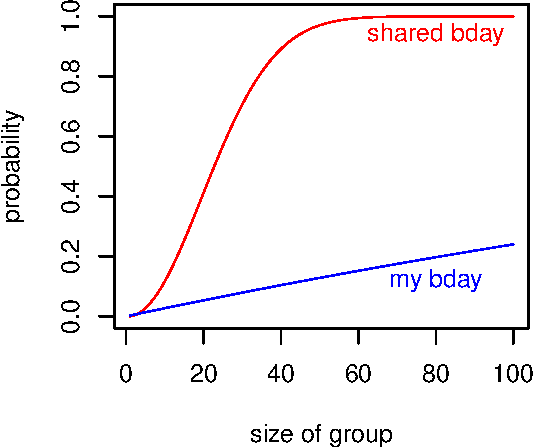
\includegraphics[keepaspectratio]{math340-notes_files/figure-latex/unnamed-chunk-136-1.pdf}}

\section{Flipping Coins with Fibonacci}\label{flipping-coins-with-fibonacci}

Let \(X\) equal the number of flips required to observe heads on consecutive flips. For instance, \(X = 6\) in the flip sequence ``T H T T H H''. The random variable \(X\) is discrete, taking on countably infinite values 2, 3, 4, \(\ldots\) .

The probability function for \(X\) is \[p(x) = \frac{F_{x+1}}{2^x} \text{     for } x = 2, 3, 4, \ldots,\] where \(F_n\) is the \(n\)th Fibonacci number. (\(F_n\) is defined recursively: \(F_1 = F_2 = 1,\) and for \(n \geq 3,\) \(F_n = F_{n-1}+F_{n-2}\).)

Deriving this function requires some satisfying work, which we work through in class.

We can also approximate the probability function by simulation.

\begin{Shaded}
\begin{Highlighting}[]
\NormalTok{trials }\OtherTok{=} \DecValTok{10000}
\NormalTok{results }\OtherTok{=} \FunctionTok{c}\NormalTok{() }\CommentTok{\#stores result}
\ControlFlowTok{for}\NormalTok{ (i }\ControlFlowTok{in} \DecValTok{1}\SpecialCharTok{:}\NormalTok{trials)\{}
\NormalTok{  flips }\OtherTok{=} \DecValTok{0}
\NormalTok{  consecutive\_H }\OtherTok{=} \DecValTok{0}
  \ControlFlowTok{while}\NormalTok{ (consecutive\_H}\SpecialCharTok{\textless{}}\DecValTok{2}\NormalTok{)\{}
\NormalTok{    flips }\OtherTok{=}\NormalTok{ flips }\SpecialCharTok{+} \DecValTok{1} \CommentTok{\#recording flips made in this trial}
\NormalTok{    consecutive\_H }\OtherTok{=} \FunctionTok{ifelse}\NormalTok{(}\FunctionTok{sample}\NormalTok{(}\FunctionTok{c}\NormalTok{(}\StringTok{"H"}\NormalTok{,}\StringTok{"T"}\NormalTok{),}\DecValTok{1}\NormalTok{)}\SpecialCharTok{==}\StringTok{"H"}\NormalTok{,consecutive\_H}\SpecialCharTok{+}\DecValTok{1}\NormalTok{,}\DecValTok{0}\NormalTok{)}
\NormalTok{  \}}
\NormalTok{  results[i]}\OtherTok{=}\NormalTok{flips }\CommentTok{\#updates results to include flips required for consec heads in this trial}
\NormalTok{\}}
\end{Highlighting}
\end{Shaded}

We note that the maximum number of flips it took to get consecutive Heads in these trials was \texttt{max(results)} = 43! (that's not a factorial symbol, just me exclaiming). So we don't list the full table of results here, just the first 10 relative frequencies, which provide estimates for the probability function:

\begin{Shaded}
\begin{Highlighting}[]
\FunctionTok{table}\NormalTok{(results)[}\DecValTok{1}\SpecialCharTok{:}\DecValTok{10}\NormalTok{]}\SpecialCharTok{/}\NormalTok{trials}
\end{Highlighting}
\end{Shaded}

\begin{verbatim}
## results
##      2      3      4      5      6      7      8      9     10     11 
## 0.2417 0.1250 0.1277 0.0952 0.0784 0.0626 0.0546 0.0395 0.0358 0.0280
\end{verbatim}

These values compare closely to the actual probability values \(F_{x+1}/2^x\):

\begin{table}
\centering
\begin{tabular}{l|l|l|l|l|l|l|l|l|l|l}
\hline
x & 2 & 3 & 4 & 5 & 6 & 7 & 8 & 9 & 10 & 11\\
\hline
Rel\_freq & 0.2417 & 0.1250 & 0.1277 & 0.0952 & 0.0784 & 0.0626 & 0.0546 & 0.0395 & 0.0358 & 0.0280\\
\hline
p(x) & 0.2500 & 0.1250 & 0.1250 & 0.0938 & 0.0781 & 0.0625 & 0.0508 & 0.0410 & 0.0332 & 0.0269\\
\hline
\end{tabular}
\end{table}

\section{Seats on an airplane}\label{seats-on-an-airplane}

\begin{quote}
A small airplane has 4 rows of 3 seats. 8 people board and sit randomly among the 12 seats. Then a couple boards. What is the probability they will be able to sit next to each other in the same row?
\end{quote}

\textbf{Strategy}

It is convenient to use a matrix with 4 rows and 3 columns to represent the seats in the plane. Each entry in the matrix is 0 or 1 depending on whether the seat is empty or occupied.

We randomly assign 8 1s to the 12 entries in the matrix, leaving the remaining 4 spots 0, and then we check to see whether one of the rows has adjacent 0s.

First, here's one way to randomly assign 8 1s and 4 0s to 12 seats (we make a vector with 8 1s and 4 0s, and then take a random permutation of it):

\begin{Shaded}
\begin{Highlighting}[]
\NormalTok{x }\OtherTok{=} \FunctionTok{sample}\NormalTok{(}\FunctionTok{rep}\NormalTok{(}\FunctionTok{c}\NormalTok{(}\DecValTok{1}\NormalTok{,}\DecValTok{0}\NormalTok{), }\FunctionTok{c}\NormalTok{(}\DecValTok{8}\NormalTok{,}\DecValTok{4}\NormalTok{)))}
\NormalTok{x}
\end{Highlighting}
\end{Shaded}

\begin{verbatim}
##  [1] 1 1 1 0 1 0 0 1 1 1 1 0
\end{verbatim}

And here's how we can store this vector of length 12 in a \(4\times 3\) matrix:

\begin{Shaded}
\begin{Highlighting}[]
\NormalTok{m}\OtherTok{=}\FunctionTok{matrix}\NormalTok{(x,}\AttributeTok{byrow=}\ConstantTok{TRUE}\NormalTok{,}\AttributeTok{nrow=}\DecValTok{4}\NormalTok{)}
\NormalTok{m}
\end{Highlighting}
\end{Shaded}

\begin{verbatim}
##      [,1] [,2] [,3]
## [1,]    1    1    1
## [2,]    0    1    0
## [3,]    0    1    1
## [4,]    1    1    0
\end{verbatim}

As the display above suggests, we can extract a value from matrix \texttt{m} by indicating its {[}row,column{]}: \texttt{m{[}3,2{]}} returns the element in row 3, column 2.

Here's one way to check for empty seats next to each other in a given row: See whether the middle entry is 0 AND the sum of the three numbers in the row is less than or equal to 1.

\begin{Shaded}
\begin{Highlighting}[]
\ControlFlowTok{for}\NormalTok{ (row }\ControlFlowTok{in} \DecValTok{1}\SpecialCharTok{:}\DecValTok{4}\NormalTok{)\{}
\NormalTok{  result}\OtherTok{=}\FunctionTok{ifelse}\NormalTok{(m[row,}\DecValTok{2}\NormalTok{] }\SpecialCharTok{==} \DecValTok{0} \SpecialCharTok{\&} \FunctionTok{sum}\NormalTok{(m[row,]) }\SpecialCharTok{\textless{}=} \DecValTok{1}\NormalTok{,}
                \StringTok{"seats together!"}\NormalTok{,}
                \StringTok{"nope"}\NormalTok{)}
   \FunctionTok{print}\NormalTok{(}\FunctionTok{paste}\NormalTok{(}\StringTok{"Row"}\NormalTok{,row,result))}
\NormalTok{\}}
\end{Highlighting}
\end{Shaded}

\begin{verbatim}
## [1] "Row 1 nope"
## [1] "Row 2 nope"
## [1] "Row 3 nope"
## [1] "Row 4 nope"
\end{verbatim}

Ok, we've got a plan! In the code below, we use \texttt{s} to record, in each trial, whether the couple can find seats together (\texttt{s} = 1) or they can't (\texttt{s} = 0).

\textbf{Final code}

\begin{Shaded}
\begin{Highlighting}[]
\NormalTok{trials }\OtherTok{=} \DecValTok{10000}
\NormalTok{results }\OtherTok{=} \FunctionTok{c}\NormalTok{()}
\ControlFlowTok{for}\NormalTok{ (i }\ControlFlowTok{in} \DecValTok{1}\SpecialCharTok{:}\NormalTok{trials)\{}
\NormalTok{  m}\OtherTok{=}\FunctionTok{matrix}\NormalTok{(}\FunctionTok{sample}\NormalTok{(}\FunctionTok{rep}\NormalTok{(}\FunctionTok{c}\NormalTok{(}\DecValTok{1}\NormalTok{,}\DecValTok{0}\NormalTok{), }\FunctionTok{c}\NormalTok{(}\DecValTok{8}\NormalTok{,}\DecValTok{4}\NormalTok{))),}\AttributeTok{byrow=}\ConstantTok{TRUE}\NormalTok{,}\AttributeTok{nrow=}\DecValTok{4}\NormalTok{)}
\NormalTok{  s }\OtherTok{=} \DecValTok{0} \CommentTok{\#assume no seats together initially}
  \ControlFlowTok{for}\NormalTok{ (r }\ControlFlowTok{in} \DecValTok{1}\SpecialCharTok{:}\DecValTok{4}\NormalTok{)\{}
    \ControlFlowTok{if}\NormalTok{ (m[r,}\DecValTok{2}\NormalTok{] }\SpecialCharTok{==} \DecValTok{0} \SpecialCharTok{\&} \FunctionTok{sum}\NormalTok{(m[r,]) }\SpecialCharTok{\textless{}=} \DecValTok{1}\NormalTok{)\{}
\NormalTok{      s }\OtherTok{=} \DecValTok{1}
      \ControlFlowTok{break} \CommentTok{\#stop the loop! We found seats together!}
\NormalTok{    \}}
\NormalTok{  \}}
\NormalTok{  results[i] }\OtherTok{=}\NormalTok{ s}
\NormalTok{\}}
\FunctionTok{sum}\NormalTok{(results)}\SpecialCharTok{/}\NormalTok{trials}
\end{Highlighting}
\end{Shaded}

\begin{verbatim}
## [1] 0.6143
\end{verbatim}

This probability seems higher than I first expected it would be, but we can also prove using our counting techniques - as an exercies - that the probability is, in fact, 20/33.

\section{Drawing names for Homemades}\label{drawing-names-for-homemades}

Growing up, I enjoyed a family tradition of exchanging homemade gifts at Christmas. In part, my enjoyment stemmed from the fact that I was the youngest person, by 6 years, in our family of 6. While I would earnestly make and give to some unlucky brother or parent a clay boot I made in the kiln at school, I was likely to receive a far superior gift in return, perhaps a lightweight springboard from my Dad that was just sturdy enough to propel my little body, flipping, into a sea of beanbags in the basement, but not sturdy enough to withstand the weight of a big brother.

I also enjoyed the secrecy of the homemades: the locked doors behind which people worked, the occasional curious scrap of material left behind on a workbench, or a splash of paint in the utility room that wasn't there earlier. Then there was the celebration of the exchange itself, the pride of giving your gift, the excitement of receiving one, and, after months of speculation, the big reveal as to who everyone drew.

We would usually draw names in late October. If anyone drew their own name, we would immediately stop the process, return all names to the hat, and try again. We kept redrawing, as necessary, until everyone drew a name that wasn't theirs. Then we were off and running, guarding the secret of our givee's identity at all costs.

In this example we pursue three questions related to the homemades:

\begin{quote}
\begin{enumerate}
\def\labelenumi{\alph{enumi})}
\tightlist
\item
  In our family of 6, what is the probability we will not have to redraw.
\end{enumerate}
\end{quote}

Our approach: Create a vector called \texttt{family}, and a permutation of \texttt{family} (called \texttt{draw}). For each \(i,\) Person \(i\) in \texttt{family} draws person \(i\) in \texttt{draw}. So, we have to redraw if the two vectors ever agree at the same location.

\begin{Shaded}
\begin{Highlighting}[]
\NormalTok{family }\OtherTok{=} \FunctionTok{c}\NormalTok{(}\StringTok{"Dad"}\NormalTok{, }\StringTok{"Mom"}\NormalTok{, }\StringTok{"Tom"}\NormalTok{, }\StringTok{"John"}\NormalTok{, }\StringTok{"Dave"}\NormalTok{, }\StringTok{"Mike"}\NormalTok{)}
\NormalTok{draw }\OtherTok{=} \FunctionTok{sample}\NormalTok{(family)}
\NormalTok{matches }\OtherTok{=} \FunctionTok{sum}\NormalTok{(family }\SpecialCharTok{==}\NormalTok{ draw) }\CommentTok{\# number of locations at which the two vectors agree}
\NormalTok{redraw }\OtherTok{=} \FunctionTok{ifelse}\NormalTok{(matches}\SpecialCharTok{==}\DecValTok{0}\NormalTok{,}\StringTok{"No."}\NormalTok{,}\StringTok{"Yes."}\NormalTok{)}
\FunctionTok{print}\NormalTok{(}\FunctionTok{paste}\NormalTok{(}\StringTok{"Redraw?"}\NormalTok{,redraw))}
\end{Highlighting}
\end{Shaded}

\begin{verbatim}
## [1] "Redraw? Yes."
\end{verbatim}

Let's check who each person drew to be sure (remember, our code is assuming the ith person in the \texttt{family} vector drew the ith person in the \texttt{draw} vector)

\begin{Shaded}
\begin{Highlighting}[]
\ControlFlowTok{for}\NormalTok{ (i }\ControlFlowTok{in} \DecValTok{1}\SpecialCharTok{:}\DecValTok{6}\NormalTok{)\{}
  \FunctionTok{print}\NormalTok{(}\FunctionTok{paste}\NormalTok{(family[i],}\StringTok{"drew"}\NormalTok{,draw[i]))}
  \ControlFlowTok{if}\NormalTok{ (family[i]}\SpecialCharTok{==}\NormalTok{draw[i])\{}
    \FunctionTok{print}\NormalTok{(}\StringTok{"Dang it! Need to redraw. Names back in the hat."}\NormalTok{) }
    \ControlFlowTok{break}\NormalTok{\}}
\NormalTok{\}}
\end{Highlighting}
\end{Shaded}

\begin{verbatim}
## [1] "Dad drew Mike"
## [1] "Mom drew Mom"
## [1] "Dang it! Need to redraw. Names back in the hat."
\end{verbatim}

We now estimate the probability of not needing to redraw as follows:

\begin{Shaded}
\begin{Highlighting}[]
\NormalTok{n}\OtherTok{=}\DecValTok{6} \CommentTok{\#size of family}
\NormalTok{family }\OtherTok{=} \DecValTok{1}\SpecialCharTok{:}\NormalTok{n }\CommentTok{\#we use numbers, to protect the innocent}
\NormalTok{trials}\OtherTok{=}\DecValTok{10000}
\NormalTok{results }\OtherTok{=} \FunctionTok{c}\NormalTok{() }\CommentTok{\#record for each trial a 0 for redraw, 1 for no redraw }
\ControlFlowTok{for}\NormalTok{ (i }\ControlFlowTok{in} \DecValTok{1}\SpecialCharTok{:}\NormalTok{trials)\{}
\NormalTok{  draw }\OtherTok{=} \FunctionTok{sample}\NormalTok{(family)}
\NormalTok{  results[i] }\OtherTok{=} \FunctionTok{ifelse}\NormalTok{(}\FunctionTok{sum}\NormalTok{(family }\SpecialCharTok{==}\NormalTok{ draw) }\SpecialCharTok{==} \DecValTok{0}\NormalTok{, }\DecValTok{1}\NormalTok{, }\DecValTok{0}\NormalTok{)}
\NormalTok{\}}
\FunctionTok{sum}\NormalTok{(results)}\SpecialCharTok{/}\NormalTok{trials}
\end{Highlighting}
\end{Shaded}

\begin{verbatim}
## [1] 0.3628
\end{verbatim}

About a 36.3 percent chance of not needing to redraw.

\begin{quote}
\begin{enumerate}
\def\labelenumi{\alph{enumi})}
\setcounter{enumi}{1}
\tightlist
\item
  What is the expected number of draws needed until we do not need to redraw?
\end{enumerate}
\end{quote}

Now in our simulation we want to redraw until we don't have to, and record how many attempts it took.

\begin{Shaded}
\begin{Highlighting}[]
\NormalTok{n}\OtherTok{=}\DecValTok{6} \CommentTok{\#size of family}
\NormalTok{family }\OtherTok{=} \DecValTok{1}\SpecialCharTok{:}\NormalTok{n }\CommentTok{\#we use numbers, to protect the innocent}
\NormalTok{trials}\OtherTok{=}\DecValTok{10000}
\NormalTok{results }\OtherTok{=} \FunctionTok{c}\NormalTok{() }\CommentTok{\#record for each trial how many attempts it took to get a good draw}
\ControlFlowTok{for}\NormalTok{ (i }\ControlFlowTok{in} \DecValTok{1}\SpecialCharTok{:}\NormalTok{trials)\{}
\NormalTok{  attempts }\OtherTok{=} \DecValTok{0}
\NormalTok{  draw\_again }\OtherTok{=} \ConstantTok{TRUE}
  \ControlFlowTok{while}\NormalTok{ (draw\_again)\{}
\NormalTok{    attempts }\OtherTok{=}\NormalTok{ attempts }\SpecialCharTok{+} \DecValTok{1}
\NormalTok{    draw }\OtherTok{=} \FunctionTok{sample}\NormalTok{(family)}
\NormalTok{    draw\_again }\OtherTok{=} \FunctionTok{sum}\NormalTok{(family }\SpecialCharTok{==}\NormalTok{ draw) }\SpecialCharTok{\textgreater{}} \DecValTok{0} \CommentTok{\# will return TRUE or FALSE}
\NormalTok{  \}}
\NormalTok{  results[i] }\OtherTok{=}\NormalTok{ attempts}
\NormalTok{\}}
\FunctionTok{barplot}\NormalTok{(}\FunctionTok{table}\NormalTok{(results))}
\end{Highlighting}
\end{Shaded}

\pandocbounded{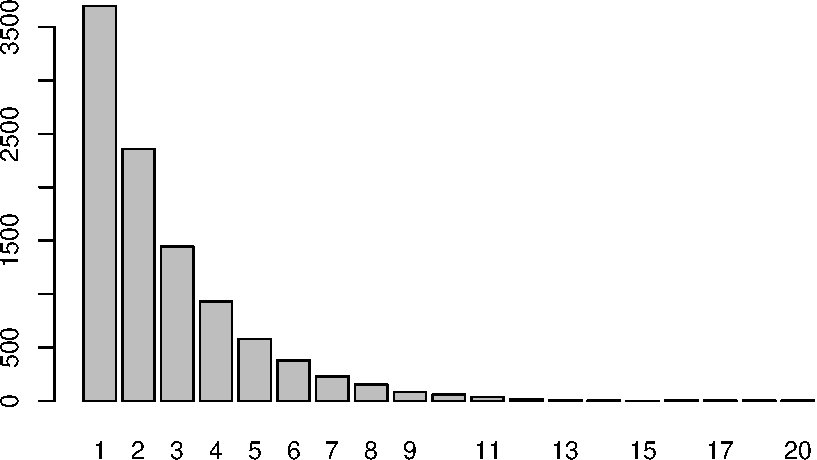
\includegraphics[keepaspectratio]{math340-notes_files/figure-latex/unnamed-chunk-147-1.pdf}}

Cripes! In 3 of the trials we needed 20 draws until no one drew their own name! Anyway, our estimate for the expected number of draws needed to get the gift-making off the mark is:

\begin{Shaded}
\begin{Highlighting}[]
\FunctionTok{sum}\NormalTok{(results)}\SpecialCharTok{/}\NormalTok{trials}
\end{Highlighting}
\end{Shaded}

\begin{verbatim}
## [1] 2.7224
\end{verbatim}

and if that number looks somewhat familiar, I encourage you to read the mathematical addendum at the end of this example.

\begin{quote}
\begin{enumerate}
\def\labelenumi{\alph{enumi})}
\setcounter{enumi}{2}
\tightlist
\item
  Over time the family grew as families do until we had 16 in the gift exchange. Does the probability of needing to redraw change substantially with the larger family size?
\end{enumerate}
\end{quote}

Let's just repeat \textbf{(b)} with \(n = 16\).

\begin{Shaded}
\begin{Highlighting}[]
\NormalTok{n}\OtherTok{=}\DecValTok{16} \CommentTok{\#size of family}
\NormalTok{family }\OtherTok{=} \DecValTok{1}\SpecialCharTok{:}\NormalTok{n }\CommentTok{\#we use numbers, to protect the innocent}
\NormalTok{trials}\OtherTok{=}\DecValTok{10000}
\NormalTok{results }\OtherTok{=} \FunctionTok{c}\NormalTok{() }\CommentTok{\#record for each trial how many attempts it took to get a good draw}
\ControlFlowTok{for}\NormalTok{ (i }\ControlFlowTok{in} \DecValTok{1}\SpecialCharTok{:}\NormalTok{trials)\{}
\NormalTok{  attempts }\OtherTok{=} \DecValTok{0}
\NormalTok{  draw\_again }\OtherTok{=} \ConstantTok{TRUE}
  \ControlFlowTok{while}\NormalTok{ (draw\_again)\{}
\NormalTok{    attempts }\OtherTok{=}\NormalTok{ attempts}\SpecialCharTok{+}\DecValTok{1}
\NormalTok{    draw }\OtherTok{=} \FunctionTok{sample}\NormalTok{(family)}
\NormalTok{    draw\_again }\OtherTok{=} \FunctionTok{sum}\NormalTok{(family }\SpecialCharTok{==}\NormalTok{ draw) }\SpecialCharTok{\textgreater{}} \DecValTok{0}
\NormalTok{  \}}
\NormalTok{  results[i] }\OtherTok{=}\NormalTok{ attempts}
\NormalTok{\}}
\FunctionTok{barplot}\NormalTok{(}\FunctionTok{table}\NormalTok{(results))}
\end{Highlighting}
\end{Shaded}

\pandocbounded{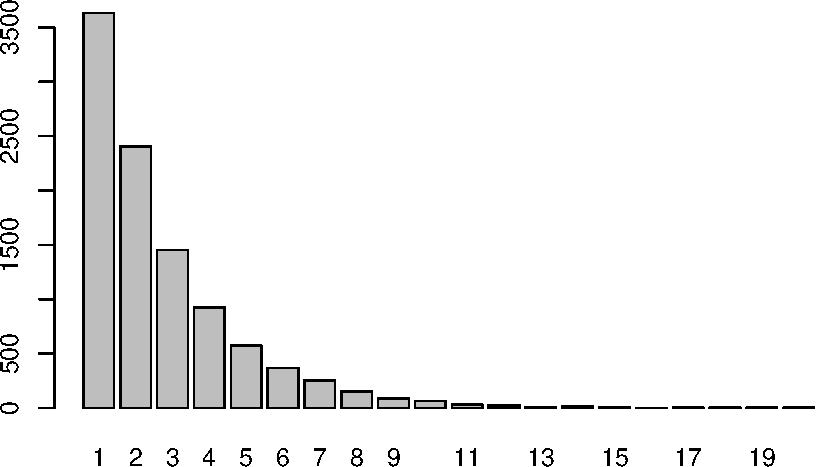
\includegraphics[keepaspectratio]{math340-notes_files/figure-latex/unnamed-chunk-149-1.pdf}}

Based on the trials, we estimate the probability of not needing a redraw in the larger family to be

\begin{Shaded}
\begin{Highlighting}[]
\FunctionTok{sum}\NormalTok{(results}\SpecialCharTok{==}\DecValTok{1}\NormalTok{)}\SpecialCharTok{/}\NormalTok{trials}
\end{Highlighting}
\end{Shaded}

\begin{verbatim}
## [1] 0.3623
\end{verbatim}

and our estimate for the expected number of draws to be

\begin{Shaded}
\begin{Highlighting}[]
\FunctionTok{sum}\NormalTok{(results)}\SpecialCharTok{/}\NormalTok{trials}
\end{Highlighting}
\end{Shaded}

\begin{verbatim}
## [1] 2.7255
\end{verbatim}

Not much movement in the estimates, it seems.

With a function and a for loop we can streamline the process for estimating both of these values for many different family sizes.

\begin{Shaded}
\begin{Highlighting}[]
\NormalTok{hat\_draw\_sim }\OtherTok{\textless{}{-}} \ControlFlowTok{function}\NormalTok{(n,trials)\{}
  \CommentTok{\# inputs: n {-} family size; trials {-} number of trials in simulation}
  \CommentTok{\# output: a vector with two values based on a number of trials:}
       \CommentTok{\# {-} first value: estimated prob of redraw for family size n}
       \CommentTok{\# {-} second value: estimated expected number of draws for family size n}
\NormalTok{  family }\OtherTok{=} \DecValTok{1}\SpecialCharTok{:}\NormalTok{n }
\NormalTok{  results }\OtherTok{=} \FunctionTok{c}\NormalTok{() }\CommentTok{\#record for each trial how many attempts it took to get a good draw}
  \ControlFlowTok{for}\NormalTok{ (i }\ControlFlowTok{in} \DecValTok{1}\SpecialCharTok{:}\NormalTok{trials)\{}
\NormalTok{    attempts }\OtherTok{=} \DecValTok{0}
\NormalTok{    draw\_again }\OtherTok{=} \ConstantTok{TRUE}
    \ControlFlowTok{while}\NormalTok{ (draw\_again)\{}
\NormalTok{      attempts }\OtherTok{=}\NormalTok{ attempts}\SpecialCharTok{+}\DecValTok{1}
\NormalTok{      draw }\OtherTok{=} \FunctionTok{sample}\NormalTok{(family)}
\NormalTok{      draw\_again }\OtherTok{=} \FunctionTok{ifelse}\NormalTok{(}\FunctionTok{sum}\NormalTok{(family }\SpecialCharTok{==}\NormalTok{ draw)}\SpecialCharTok{\textgreater{}}\DecValTok{0}\NormalTok{,}\ConstantTok{TRUE}\NormalTok{,}\ConstantTok{FALSE}\NormalTok{)}
\NormalTok{    \}}
\NormalTok{    results[i] }\OtherTok{=}\NormalTok{ attempts}
\NormalTok{  \}}
  \FunctionTok{return}\NormalTok{(}\FunctionTok{c}\NormalTok{(}\FunctionTok{sum}\NormalTok{(results}\SpecialCharTok{==}\DecValTok{1}\NormalTok{)}\SpecialCharTok{/}\NormalTok{trials,}\FunctionTok{sum}\NormalTok{(results)}\SpecialCharTok{/}\NormalTok{trials))}
\NormalTok{\}}
\end{Highlighting}
\end{Shaded}

\begin{Shaded}
\begin{Highlighting}[]
\CommentTok{\# run simulation for various family sizes}
\NormalTok{family\_size }\OtherTok{=} \FunctionTok{c}\NormalTok{(}\DecValTok{2}\SpecialCharTok{:}\DecValTok{10}\NormalTok{,}\FunctionTok{seq}\NormalTok{(}\DecValTok{15}\NormalTok{,}\DecValTok{60}\NormalTok{,}\DecValTok{5}\NormalTok{))}
\NormalTok{prob\_redraw }\OtherTok{=} \FunctionTok{c}\NormalTok{()}
\NormalTok{expected\_draws }\OtherTok{=} \FunctionTok{c}\NormalTok{()}
\ControlFlowTok{for}\NormalTok{ (i }\ControlFlowTok{in} \DecValTok{1}\SpecialCharTok{:}\FunctionTok{length}\NormalTok{(family\_size))\{}
\NormalTok{  v}\OtherTok{=}\FunctionTok{hat\_draw\_sim}\NormalTok{(family\_size[i],}\AttributeTok{trials=}\DecValTok{10000}\NormalTok{)}
\NormalTok{  prob\_redraw[i] }\OtherTok{=}\NormalTok{ v[}\DecValTok{1}\NormalTok{]}
\NormalTok{  expected\_draws[i] }\OtherTok{=}\NormalTok{ v[}\DecValTok{2}\NormalTok{]}
\NormalTok{\}}
\CommentTok{\#table of results}
\FunctionTok{kbl}\NormalTok{(}\FunctionTok{data.frame}\NormalTok{(family\_size,prob\_redraw,expected\_draws)) }\SpecialCharTok{\%\textgreater{}\%} \FunctionTok{kable\_styling}\NormalTok{(}\AttributeTok{full\_width=}\ConstantTok{FALSE}\NormalTok{)}
\end{Highlighting}
\end{Shaded}

\begin{table}
\centering
\begin{tabular}[t]{r|r|r}
\hline
family\_size & prob\_redraw & expected\_draws\\
\hline
2 & 0.5002 & 2.0022\\
\hline
3 & 0.3313 & 3.0560\\
\hline
4 & 0.3661 & 2.6887\\
\hline
5 & 0.3617 & 2.7340\\
\hline
6 & 0.3729 & 2.7007\\
\hline
7 & 0.3671 & 2.7236\\
\hline
8 & 0.3697 & 2.7416\\
\hline
9 & 0.3678 & 2.6965\\
\hline
10 & 0.3639 & 2.6905\\
\hline
15 & 0.3634 & 2.7022\\
\hline
20 & 0.3622 & 2.7196\\
\hline
25 & 0.3699 & 2.7072\\
\hline
30 & 0.3714 & 2.7097\\
\hline
35 & 0.3741 & 2.6838\\
\hline
40 & 0.3669 & 2.7263\\
\hline
45 & 0.3589 & 2.7252\\
\hline
50 & 0.3690 & 2.7091\\
\hline
55 & 0.3699 & 2.7262\\
\hline
60 & 0.3731 & 2.6993\\
\hline
\end{tabular}
\end{table}

It seems the probability of not needing a redraw and the expected number of draws needed both converge fairly quickly to about 0.37ish and 2.7 ish, respectively.

In fact, these values ought to be closely related of one another since ``drawing until our first success'' sounds like a geometric distribution to me. The probability of success on any given draw somewher in the neighborhood of \(p = .37,\) and the expected value for a geometric distribution is \(1/p,\) which would be about \(1/.37,\) which puts us in the neighborhood of \(2.7\).
If these numbers seem frustratingly imprecise, I'm glad, and I invite you to read the following addendum.

\subsection*{Mathematical addendum to the question of drawing names.}\label{mathematical-addendum-to-the-question-of-drawing-names.}
\addcontentsline{toc}{subsection}{Mathematical addendum to the question of drawing names.}

The actual expected number of draws, as \(n \to \infty,\) is \(e,\) and the probability of not needing to redraw approaches \(1/e\) as \(n \to \infty\).

In part (a) of this question, we are counting derangements of a vector.
A \textbf{derangement}\index{permutation!derangement} of a vector is a permutation of it in which no element is in its original position. An element of a permutation is called \emph{fixed points}\index{permutation!fixed point} if it appears in its original position, so a derangement of a vector is a permutation of it with no fixed points. In part (a) we are estimating the probability that a permutation of the \texttt{family} vector is a derangement. There is a nice recursive formula for the number of derangements of a vector of size \(n,\) and it can be used to prove that the probability of drawing a derangement converges to \(1/e\) as \(n \to \infty\).

\section{Idiot's Delight}\label{idiots-delight}

Idiot's delight\index{idiot's delight} is a simple card game without strategy or game play options. Here are the rules:

At the start of the game your \emph{hand} is empty, and the full deck is the \emph{draw pile}. Your hand will always be an ordered list of cards.

Each turn consists of two steps.

\begin{enumerate}
\def\labelenumi{\arabic{enumi}.}
\tightlist
\item
  \emph{Draw one card} from the draw pile. This card becomes the first, or ``top'' card in your hand.
\item
  \emph{Check for hand reductions}. If you have fewer than 4 cards in your hand you can make no reductions. If you have at least four cards, compare the top card with the fourth card in your hand (fourth from the top). If these cards have the same rank, remove the top four cards from your hand. If these cards have the same suit, remove the two cards in between (so, the 2nd and 3rd cards in your hand). Repeat step 2 until no reduction can be made. When no reduction can be made begin the next turn.
\end{enumerate}

The game ends after you have drawn all cards from the deck and you can make no reductions. Your \emph{game score} is the size of your hand at the end. For a regular 52 card deck you \emph{win} if your score is less than 10.

We have two questions about this game.

\begin{quote}
\begin{enumerate}
\def\labelenumi{\alph{enumi})}
\tightlist
\item
  Estimate the probability that you win.
\end{enumerate}
\end{quote}

\begin{quote}
\begin{enumerate}
\def\labelenumi{\alph{enumi})}
\setcounter{enumi}{1}
\tightlist
\item
  Estimate how likely a player will have a reduction on each of the 52 draws that constitute a game.
\end{enumerate}
\end{quote}

Creating this game in R requires some work, beginning with the creation of a deck of cards, and continuing with the creation of some functions to manage the game play. Playing the game for a while might help the reader make sense of the code below.

\begin{Shaded}
\begin{Highlighting}[]
\CommentTok{\#Build a Deck }
\NormalTok{rank }\OtherTok{=} \FunctionTok{rep}\NormalTok{(}\FunctionTok{c}\NormalTok{(}\DecValTok{2}\SpecialCharTok{:}\DecValTok{10}\NormalTok{,}\StringTok{"J"}\NormalTok{,}\StringTok{"Q"}\NormalTok{,}\StringTok{"K"}\NormalTok{,}\StringTok{"A"}\NormalTok{),}\DecValTok{4}\NormalTok{)}
\NormalTok{suit }\OtherTok{=} \FunctionTok{c}\NormalTok{(}\FunctionTok{rep}\NormalTok{(}\StringTok{"clubs"}\NormalTok{,}\DecValTok{13}\NormalTok{),}\FunctionTok{rep}\NormalTok{(}\StringTok{"diamonds"}\NormalTok{,}\DecValTok{13}\NormalTok{),}\FunctionTok{rep}\NormalTok{(}\StringTok{"hearts"}\NormalTok{,}\DecValTok{13}\NormalTok{),}\FunctionTok{rep}\NormalTok{(}\StringTok{"spades"}\NormalTok{,}\DecValTok{13}\NormalTok{))}
\NormalTok{deck }\OtherTok{=} \FunctionTok{paste0}\NormalTok{(rank,}\StringTok{"{-}"}\NormalTok{,suit) }\CommentTok{\#standard deck of cards}
\FunctionTok{sample}\NormalTok{(deck,}\DecValTok{4}\NormalTok{) }\CommentTok{\#display four random cards}
\end{Highlighting}
\end{Shaded}

\begin{verbatim}
## [1] "2-hearts" "5-spades" "3-clubs"  "J-clubs"
\end{verbatim}

Here's code for playing the game with a lot of printed statements to increase the drama of each turn. We do not run the code here, but recommend you copy and paste it into a script in your own session and play a few times to get the feel for it.

\begin{Shaded}
\begin{Highlighting}[]
\CommentTok{\#build a deck}
\NormalTok{rank }\OtherTok{=} \FunctionTok{rep}\NormalTok{(}\FunctionTok{c}\NormalTok{(}\DecValTok{2}\SpecialCharTok{:}\DecValTok{10}\NormalTok{,}\StringTok{"J"}\NormalTok{,}\StringTok{"Q"}\NormalTok{,}\StringTok{"K"}\NormalTok{,}\StringTok{"A"}\NormalTok{),}\DecValTok{4}\NormalTok{)}
\NormalTok{suit }\OtherTok{=} \FunctionTok{c}\NormalTok{(}\FunctionTok{rep}\NormalTok{(}\StringTok{"clubs"}\NormalTok{,}\DecValTok{13}\NormalTok{),}\FunctionTok{rep}\NormalTok{(}\StringTok{"diamonds"}\NormalTok{,}\DecValTok{13}\NormalTok{),}\FunctionTok{rep}\NormalTok{(}\StringTok{"hearts"}\NormalTok{,}\DecValTok{13}\NormalTok{),}\FunctionTok{rep}\NormalTok{(}\StringTok{"spades"}\NormalTok{,}\DecValTok{13}\NormalTok{))}
\NormalTok{deck }\OtherTok{=} \FunctionTok{paste0}\NormalTok{(rank,}\StringTok{"{-}"}\NormalTok{,suit)}

\CommentTok{\#game functions}
\NormalTok{rank }\OtherTok{\textless{}{-}} \ControlFlowTok{function}\NormalTok{(card)\{ }\CommentTok{\#extracts the rank from the card string}
  \FunctionTok{return}\NormalTok{(}\FunctionTok{unlist}\NormalTok{(}\FunctionTok{strsplit}\NormalTok{(card,}\StringTok{"{-}"}\NormalTok{))[}\DecValTok{1}\NormalTok{])}
\NormalTok{\}}
\NormalTok{suit }\OtherTok{\textless{}{-}} \ControlFlowTok{function}\NormalTok{(card)\{ }\CommentTok{\#extracts the suit from the card string}
  \FunctionTok{return}\NormalTok{(}\FunctionTok{unlist}\NormalTok{(}\FunctionTok{strsplit}\NormalTok{(card,}\StringTok{"{-}"}\NormalTok{))[}\DecValTok{2}\NormalTok{])}
\NormalTok{\}}
\NormalTok{scan }\OtherTok{\textless{}{-}} \ControlFlowTok{function}\NormalTok{(hand)\{ }\CommentTok{\#scans the hand for hand reductions}
  \ControlFlowTok{if}\NormalTok{ (}\FunctionTok{length}\NormalTok{(hand) }\SpecialCharTok{\textless{}=} \DecValTok{3}\NormalTok{)\{}\FunctionTok{return}\NormalTok{(hand)\}}
  \ControlFlowTok{if}\NormalTok{ (}\FunctionTok{rank}\NormalTok{(hand[}\DecValTok{1}\NormalTok{])}\SpecialCharTok{==}\FunctionTok{rank}\NormalTok{(hand[}\DecValTok{4}\NormalTok{]))\{}\FunctionTok{return}\NormalTok{(hand[}\SpecialCharTok{{-}}\NormalTok{(}\DecValTok{1}\SpecialCharTok{:}\DecValTok{4}\NormalTok{)])\}}
  \ControlFlowTok{if}\NormalTok{ (}\FunctionTok{suit}\NormalTok{(hand[}\DecValTok{1}\NormalTok{])}\SpecialCharTok{==}\FunctionTok{suit}\NormalTok{(hand[}\DecValTok{4}\NormalTok{]))\{}
\NormalTok{      hand }\OtherTok{\textless{}{-}}\NormalTok{ hand[}\SpecialCharTok{{-}}\NormalTok{(}\DecValTok{2}\SpecialCharTok{:}\DecValTok{3}\NormalTok{)]}
\NormalTok{      hand }\OtherTok{\textless{}{-}} \FunctionTok{scan}\NormalTok{(hand)}
\NormalTok{  \}}
  \FunctionTok{return}\NormalTok{(hand)}
\NormalTok{\}}

\CommentTok{\#play game with commentary}
\NormalTok{hand }\OtherTok{=} \FunctionTok{c}\NormalTok{()}
\NormalTok{draw\_pile }\OtherTok{=} \FunctionTok{sample}\NormalTok{(deck)}\CommentTok{\#shuffles the deck}
\ControlFlowTok{for}\NormalTok{ (k }\ControlFlowTok{in} \DecValTok{1}\SpecialCharTok{:}\FunctionTok{length}\NormalTok{(deck))\{}
  \FunctionTok{print}\NormalTok{(}\FunctionTok{paste}\NormalTok{(}\StringTok{"Turn"}\NormalTok{,k,}\StringTok{"hand after draw but before scanning:"}\NormalTok{))}
\NormalTok{  hand }\OtherTok{\textless{}{-}} \FunctionTok{c}\NormalTok{(draw\_pile[k],hand) }\CommentTok{\#add card to hand}
  \FunctionTok{print}\NormalTok{(hand)}
\NormalTok{  hand }\OtherTok{\textless{}{-}} \FunctionTok{scan}\NormalTok{(hand)}
  \FunctionTok{print}\NormalTok{(}\StringTok{\textquotesingle{}=================\textquotesingle{}}\NormalTok{)}
\NormalTok{\}}
\FunctionTok{print}\NormalTok{(}\FunctionTok{paste}\NormalTok{(}\StringTok{"Game score:"}\NormalTok{,}\FunctionTok{length}\NormalTok{(hand)))}
\end{Highlighting}
\end{Shaded}

Here's a play game function that plays the game (without commentary) and returns the size of your hand after each turn.

\begin{Shaded}
\begin{Highlighting}[]
\NormalTok{play\_game }\OtherTok{\textless{}{-}} \ControlFlowTok{function}\NormalTok{()\{}
  \CommentTok{\#build a deck}
\NormalTok{  rank }\OtherTok{=} \FunctionTok{rep}\NormalTok{(}\FunctionTok{c}\NormalTok{(}\DecValTok{2}\SpecialCharTok{:}\DecValTok{10}\NormalTok{,}\StringTok{"J"}\NormalTok{,}\StringTok{"Q"}\NormalTok{,}\StringTok{"K"}\NormalTok{,}\StringTok{"A"}\NormalTok{),}\DecValTok{4}\NormalTok{)}
\NormalTok{  suit }\OtherTok{=} \FunctionTok{c}\NormalTok{(}\FunctionTok{rep}\NormalTok{(}\StringTok{"clubs"}\NormalTok{,}\DecValTok{13}\NormalTok{),}\FunctionTok{rep}\NormalTok{(}\StringTok{"diamonds"}\NormalTok{,}\DecValTok{13}\NormalTok{),}\FunctionTok{rep}\NormalTok{(}\StringTok{"hearts"}\NormalTok{,}\DecValTok{13}\NormalTok{),}\FunctionTok{rep}\NormalTok{(}\StringTok{"spades"}\NormalTok{,}\DecValTok{13}\NormalTok{))}
\NormalTok{  deck }\OtherTok{=} \FunctionTok{paste0}\NormalTok{(rank,}\StringTok{"{-}"}\NormalTok{,suit)}
  
  \CommentTok{\#game functions}
\NormalTok{  rank }\OtherTok{\textless{}{-}} \ControlFlowTok{function}\NormalTok{(card)\{ }\CommentTok{\#extracts the rank from the card string}
    \FunctionTok{return}\NormalTok{(}\FunctionTok{unlist}\NormalTok{(}\FunctionTok{strsplit}\NormalTok{(card,}\StringTok{"{-}"}\NormalTok{))[}\DecValTok{1}\NormalTok{])}
\NormalTok{    \}}
\NormalTok{  suit }\OtherTok{\textless{}{-}} \ControlFlowTok{function}\NormalTok{(card)\{ }\CommentTok{\#extracts the suit from the card string}
    \FunctionTok{return}\NormalTok{(}\FunctionTok{unlist}\NormalTok{(}\FunctionTok{strsplit}\NormalTok{(card,}\StringTok{"{-}"}\NormalTok{))[}\DecValTok{2}\NormalTok{])}
\NormalTok{    \}}
\NormalTok{  scan }\OtherTok{\textless{}{-}} \ControlFlowTok{function}\NormalTok{(hand)\{ }\CommentTok{\#scans the hand for hand reductions}
    \ControlFlowTok{if}\NormalTok{ (}\FunctionTok{length}\NormalTok{(hand) }\SpecialCharTok{\textless{}=} \DecValTok{3}\NormalTok{)\{}\FunctionTok{return}\NormalTok{(hand)\}}
    \ControlFlowTok{if}\NormalTok{ (}\FunctionTok{rank}\NormalTok{(hand[}\DecValTok{1}\NormalTok{])}\SpecialCharTok{==}\FunctionTok{rank}\NormalTok{(hand[}\DecValTok{4}\NormalTok{]))\{}\FunctionTok{return}\NormalTok{(hand[}\SpecialCharTok{{-}}\NormalTok{(}\DecValTok{1}\SpecialCharTok{:}\DecValTok{4}\NormalTok{)])\}}
    \ControlFlowTok{if}\NormalTok{ (}\FunctionTok{suit}\NormalTok{(hand[}\DecValTok{1}\NormalTok{])}\SpecialCharTok{==}\FunctionTok{suit}\NormalTok{(hand[}\DecValTok{4}\NormalTok{]))\{}
\NormalTok{      hand }\OtherTok{\textless{}{-}}\NormalTok{ hand[}\SpecialCharTok{{-}}\NormalTok{(}\DecValTok{2}\SpecialCharTok{:}\DecValTok{3}\NormalTok{)]}
\NormalTok{      hand }\OtherTok{\textless{}{-}} \FunctionTok{scan}\NormalTok{(hand)}
\NormalTok{      \}}
    \FunctionTok{return}\NormalTok{(hand)}
\NormalTok{    \}}
  \CommentTok{\#play game without comment, returning vector of hand\_sizes}
\NormalTok{  hand }\OtherTok{=} \FunctionTok{c}\NormalTok{()}
\NormalTok{  draw\_pile }\OtherTok{=} \FunctionTok{sample}\NormalTok{(deck)}\CommentTok{\#shuffles the deck}
\NormalTok{  hand\_size }\OtherTok{=} \FunctionTok{c}\NormalTok{()}
  \ControlFlowTok{for}\NormalTok{ (k }\ControlFlowTok{in} \DecValTok{1}\SpecialCharTok{:}\FunctionTok{length}\NormalTok{(deck))\{}
\NormalTok{    hand }\OtherTok{\textless{}{-}} \FunctionTok{c}\NormalTok{(draw\_pile[k],hand) }\CommentTok{\#add card to hand}
\NormalTok{    hand }\OtherTok{\textless{}{-}} \FunctionTok{scan}\NormalTok{(hand) }\CommentTok{\#look for reductions}
\NormalTok{    hand\_size[k]}\OtherTok{=}\FunctionTok{length}\NormalTok{(hand) }\CommentTok{\#record length of hand after turn k}
\NormalTok{    \}}
  \FunctionTok{return}\NormalTok{(hand\_size)}
\NormalTok{\}}
\end{Highlighting}
\end{Shaded}

Now we do our simulations. The result of running the \texttt{play\_game()} function is a vector of length 52, indicating the size of our hand after each of our 52 draws. With the trials below, we concatenate these vectors into one long vector \texttt{results} (of length \texttt{52*trials}) which we then convert into matrix with 52 columns in such a way that each row of the matrix represents the hand sizes for a single game.

\begin{Shaded}
\begin{Highlighting}[]
\NormalTok{trials }\OtherTok{=} \DecValTok{1000}
\NormalTok{results }\OtherTok{=} \FunctionTok{c}\NormalTok{()}
\ControlFlowTok{for}\NormalTok{ (i }\ControlFlowTok{in} \DecValTok{1}\SpecialCharTok{:}\NormalTok{trials)\{}
\NormalTok{  v }\OtherTok{=} \FunctionTok{play\_game}\NormalTok{() }
\NormalTok{  results }\OtherTok{=} \FunctionTok{c}\NormalTok{(results,v)}
\NormalTok{\}}
\NormalTok{M }\OtherTok{=} \FunctionTok{matrix}\NormalTok{(results,}\AttributeTok{byrow =} \ConstantTok{TRUE}\NormalTok{,}\AttributeTok{ncol =} \DecValTok{52}\NormalTok{)}
\end{Highlighting}
\end{Shaded}

The last column of this matrix records each of our final game scores, so the fraction of those values less than 10 answer part (a) for us.

Our estimated probability of winning in a game of Idiot's delight:

\begin{Shaded}
\begin{Highlighting}[]
\FunctionTok{sum}\NormalTok{(M[,}\DecValTok{52}\NormalTok{]}\SpecialCharTok{\textless{}}\DecValTok{10}\NormalTok{)}\SpecialCharTok{/}\NormalTok{trials}
\end{Highlighting}
\end{Shaded}

\begin{verbatim}
## [1] 0.333
\end{verbatim}

For (b), the likelihood of having a reduction on turn \(k\) (for each \(k = 1,2,\ldots 52\)), we can compare our hand size after turn \(k\) with our hand size after turn \(k-1\).

We know turns \(k = 1, 2, 3\) can have no reductions, but starting with \(k = 4\) we might:

\begin{Shaded}
\begin{Highlighting}[]
\NormalTok{reduction }\OtherTok{=} \FunctionTok{c}\NormalTok{(}\DecValTok{0}\NormalTok{,}\DecValTok{0}\NormalTok{,}\DecValTok{0}\NormalTok{) }\CommentTok{\# start by recording 0 reductions for turns 1,2,3}
\ControlFlowTok{for}\NormalTok{ (k }\ControlFlowTok{in} \DecValTok{4}\SpecialCharTok{:}\DecValTok{52}\NormalTok{)\{}
\NormalTok{  reduction[k] }\OtherTok{=} \FunctionTok{sum}\NormalTok{(M[,k]}\SpecialCharTok{\textless{}}\NormalTok{M[,k}\DecValTok{{-}1}\NormalTok{])}
\NormalTok{\}}
\FunctionTok{plot}\NormalTok{(}\AttributeTok{x=}\DecValTok{1}\SpecialCharTok{:}\DecValTok{52}\NormalTok{,}\AttributeTok{y=}\NormalTok{reduction}\SpecialCharTok{/}\NormalTok{trials,}\AttributeTok{type=}\StringTok{\textquotesingle{}l\textquotesingle{}}\NormalTok{)}
\end{Highlighting}
\end{Shaded}

\pandocbounded{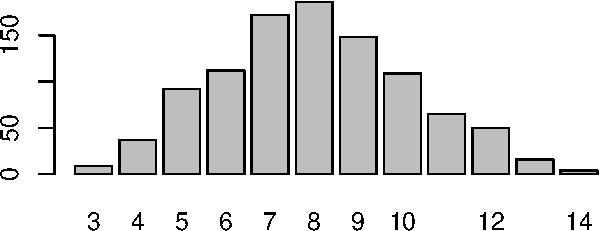
\includegraphics[keepaspectratio]{math340-notes_files/figure-latex/unnamed-chunk-159-1.pdf}}

Starting with turn 4 it looks like the likelihood of having a reduction stays roughly constant, at about 0.28.

\chapter{Discrete Random Variables in R}\label{R-discreteRV}

Here we investigate in R the common, named discrete random variables we encounter in MATH 340:

\begin{itemize}
\tightlist
\item
  \hyperref[binomialR]{binomial} \textbar{} \texttt{binom}
\item
  \hyperref[geometricR]{geometric} \textbar{} \texttt{geom}
\item
  \hyperref[negbinomR]{negative binomial} \textbar{} \texttt{nbinom}
\item
  \hyperref[hyperR]{hypergeometric} \textbar{} \texttt{hyper}
\item
  \hyperref[poissonR]{Poisson} \textbar{} \texttt{pois}
\end{itemize}

We use four commands to work with the named distributions. For a distribution named \texttt{\_\_\_}:

\begin{itemize}
\tightlist
\item
  \texttt{d\_\_\_(x,...)} \textbar{} probability function, \(p(x)\)
\item
  \texttt{p\_\_\_(q,...)} \textbar{} Cumulative probability, \(P(X \leq q)\)
\item
  \texttt{q\_\_\_(p,...)} \textbar{} Quantiles, finds \(x\) such that \(P(X \leq x) = p\)
\item
  \texttt{r\_\_\_(n,...)} \textbar{} Random sample of size \(n\) from the distribution
\end{itemize}

We also discuss below how to build and analyze \hyperref[custom-discrete-R]{homemade discrete random variables in R}.

\section{\texorpdfstring{Binomial \texttt{binom}}{Binomial binom}}\label{binomialR}

\textbf{The Scene}

Recall, \(X \sim \texttt{binom}(n,p)\) means \(X\) counts the number of successes in \(n\) independent, identical Bernoulli trials, when probability of success on any given trial is \(p\).

\textbf{The space of \(X\)} is \(x = 0, 1, \ldots, n\).

\textbf{Probability function}\\
For \(x = 0, 1, \ldots, n,\) \[p(x)=\binom{n}{x}p^x(1-p)^{n-x}.\]

\textbf{The binomial distribution in R}

\subsection*{\texorpdfstring{\texttt{dbinom()} - probability function}{dbinom() - probability function}}\label{dbinom---probability-function}
\addcontentsline{toc}{subsection}{\texttt{dbinom()} - probability function}

\begin{quote}
\texttt{dbinom(x,n,p)} returns the probability \(P(X = x)\) for \(X \sim \texttt{binom}(n,p)\).
\end{quote}

For instance, \texttt{dbinom(2,5,.3)} returns \[\binom{5}{2}(.3)^2(.7)^3.\]

\begin{Shaded}
\begin{Highlighting}[]
\FunctionTok{dbinom}\NormalTok{(}\DecValTok{2}\NormalTok{,}\DecValTok{5}\NormalTok{,.}\DecValTok{3}\NormalTok{)}
\end{Highlighting}
\end{Shaded}

\begin{verbatim}
## [1] 0.3087
\end{verbatim}

As a check:

\begin{Shaded}
\begin{Highlighting}[]
\FunctionTok{choose}\NormalTok{(}\DecValTok{5}\NormalTok{,}\DecValTok{2}\NormalTok{)}\SpecialCharTok{*}\NormalTok{(.}\DecValTok{3}\NormalTok{)}\SpecialCharTok{\^{}}\DecValTok{2}\SpecialCharTok{*}\NormalTok{(.}\DecValTok{7}\NormalTok{)}\SpecialCharTok{\^{}}\DecValTok{3}
\end{Highlighting}
\end{Shaded}

\begin{verbatim}
## [1] 0.3087
\end{verbatim}

\subsection*{\texorpdfstring{\texttt{pbinom()} - cumulative probability}{pbinom() - cumulative probability}}\label{pbinom---cumulative-probability}
\addcontentsline{toc}{subsection}{\texttt{pbinom()} - cumulative probability}

\begin{quote}
\texttt{pbinom(q,n,p)}returns the cumulative probability \(P(X \leq q)\) for \(X \sim \text{binom}(n,p)\): \[\sum_{x=0}^q p(x)=\sum_{x=0}^q\binom{n}{x}p^x(1-p)^{n-x}.\]
\end{quote}

So \texttt{pbinom(2,5,.3)} returns \(P(X \leq 2)\) when \(X\) is \(\texttt{binom}(5,.3)\):

\begin{Shaded}
\begin{Highlighting}[]
\FunctionTok{pbinom}\NormalTok{(}\DecValTok{2}\NormalTok{,}\DecValTok{5}\NormalTok{,.}\DecValTok{3}\NormalTok{)}
\end{Highlighting}
\end{Shaded}

\begin{verbatim}
## [1] 0.83692
\end{verbatim}

As a check:

\begin{Shaded}
\begin{Highlighting}[]
\FunctionTok{dbinom}\NormalTok{(}\DecValTok{0}\NormalTok{,}\DecValTok{5}\NormalTok{,.}\DecValTok{3}\NormalTok{)}\SpecialCharTok{+}\FunctionTok{dbinom}\NormalTok{(}\DecValTok{1}\NormalTok{,}\DecValTok{5}\NormalTok{,.}\DecValTok{3}\NormalTok{)}\SpecialCharTok{+}\FunctionTok{dbinom}\NormalTok{(}\DecValTok{2}\NormalTok{,}\DecValTok{5}\NormalTok{,.}\DecValTok{3}\NormalTok{)}
\end{Highlighting}
\end{Shaded}

\begin{verbatim}
## [1] 0.83692
\end{verbatim}

\subsection*{\texorpdfstring{\texttt{qbinom()} - quantiles}{qbinom() - quantiles}}\label{qbinom---quantiles}
\addcontentsline{toc}{subsection}{\texttt{qbinom()} - quantiles}

Recall the definition of quantile (\ref{def:quantile}): If \(0 < p < 1,\) the \(p\)th quantile of \(X,\) denoted \(\phi_p,\) is the smallest value such that \(P(X \leq \phi_p) \geq p\). In other words, the value \(\phi_p\) marks the smallest value below which one finds 100*p percent of the distribution of \(X\).

\begin{quote}
\texttt{qbinom(q,n,p)} returns the quantile \(\phi_q\) for \(X \sim \texttt{binom}(n,p)\)
\end{quote}

For instance, what value marks the 95th percentile of the \(\texttt{binom}(100,.5)\) distribution?

\begin{Shaded}
\begin{Highlighting}[]
\FunctionTok{qbinom}\NormalTok{(.}\DecValTok{95}\NormalTok{,}\DecValTok{100}\NormalTok{,.}\DecValTok{5}\NormalTok{)}
\end{Highlighting}
\end{Shaded}

\begin{verbatim}
## [1] 58
\end{verbatim}

So, if you flip a fair coin 100 times and count how many heads you get, about 95\% of the time you would flip less than or equal to 58 heads.

We can check this:

\begin{Shaded}
\begin{Highlighting}[]
\FunctionTok{pbinom}\NormalTok{(}\DecValTok{58}\NormalTok{,}\DecValTok{100}\NormalTok{,.}\DecValTok{5}\NormalTok{)}
\end{Highlighting}
\end{Shaded}

\begin{verbatim}
## [1] 0.955687
\end{verbatim}

\subsection*{\texorpdfstring{\texttt{rbinom()} - sampling}{rbinom() - sampling}}\label{rbinom---sampling}
\addcontentsline{toc}{subsection}{\texttt{rbinom()} - sampling}

\begin{quote}
\texttt{rbinom(10,20,.4)} will generate a vector that stores a random sample of size 10 drawn from a \(\texttt{binom}(20,.4)\) distribution.
\end{quote}

\begin{Shaded}
\begin{Highlighting}[]
\FunctionTok{rbinom}\NormalTok{(}\DecValTok{10}\NormalTok{,}\DecValTok{20}\NormalTok{,.}\DecValTok{4}\NormalTok{)}
\end{Highlighting}
\end{Shaded}

\begin{verbatim}
##  [1] 10 10  7  7  6  7 10  6  4  7
\end{verbatim}

We can use \texttt{r\_\_\_} to run simulations, and to visualize the shape of a distribution.

Two useful commands for summarizing data: \texttt{table()} presents the frequency table for the sample, and \texttt{barplot(table())} is a quick way to visualize this frequency table.

\begin{Shaded}
\begin{Highlighting}[]
\NormalTok{sim\_data }\OtherTok{=} \FunctionTok{rbinom}\NormalTok{(}\DecValTok{1000}\NormalTok{,}\DecValTok{20}\NormalTok{,.}\DecValTok{4}\NormalTok{) }\CommentTok{\# sample of size 1000 from binom(20,.4).}
\FunctionTok{table}\NormalTok{(sim\_data)}
\end{Highlighting}
\end{Shaded}

\begin{verbatim}
## sim_data
##   2   3   4   5   6   7   8   9  10  11  12  13  14 
##   2  22  41  86 123 152 164 157 118  74  35  22   4
\end{verbatim}

\begin{Shaded}
\begin{Highlighting}[]
\FunctionTok{barplot}\NormalTok{(}\FunctionTok{table}\NormalTok{(sim\_data))}
\end{Highlighting}
\end{Shaded}

\pandocbounded{\includegraphics[keepaspectratio]{math340-notes_files/figure-latex/unnamed-chunk-168-1.pdf}}

\section{\texorpdfstring{Geometric \texttt{geom}}{Geometric geom}}\label{geometricR}

\textbf{The Scene}\\
Let the random variable \(X\) denote the number of identical, independent Bernoulli trials (with probability of success \(p,\) probability of failure \(q = 1-p\)) up to and including the first success.
Then \(X\) is called a \emph{geometric random variable} with parameter \(p\).

\textbf{Notation}\\
\(X\) is \texttt{geom}\((p)\).

\textbf{The space of \(X\)} is \(x = 1, 2, \ldots\)

\textbf{Probability function}\\
For \(x = 1, 2, 3, \ldots,\) \[p(x)= q^{x-1}p.\]

\textbf{NOTE}: The geometric distribution in R counts failures, not total trials.

In R \texttt{geom} counts the number of failures until the first success, not the total number of trials up to and including the first success.

As with the \texttt{binom} distribution, we can use the \texttt{d\_\_\_}, \texttt{p\_\_\_}, \texttt{q\_\_\_}, and \texttt{r\_\_\_} commands to determine probability for particular values of \(x,\) cumulative probabilities, quantiles, and random samples, respectively.

\begin{quote}
\texttt{dgeom(4,.3)} gives the probability of seeing 4 failures before the first success in a Bernoulli trial in which \(p = .3\)
\end{quote}

\begin{Shaded}
\begin{Highlighting}[]
\FunctionTok{dgeom}\NormalTok{(}\DecValTok{4}\NormalTok{,.}\DecValTok{3}\NormalTok{)}
\end{Highlighting}
\end{Shaded}

\begin{verbatim}
## [1] 0.07203
\end{verbatim}

\begin{quote}
\texttt{pgeom(4,.3)} gives the probability of seeing 4 or fewer failures before the first success in a sequence of Bernoulli trials in which \(p = .3\)
\end{quote}

\begin{Shaded}
\begin{Highlighting}[]
\FunctionTok{pgeom}\NormalTok{(}\DecValTok{4}\NormalTok{,.}\DecValTok{3}\NormalTok{)}
\end{Highlighting}
\end{Shaded}

\begin{verbatim}
## [1] 0.83193
\end{verbatim}

and the following line gives the probability of seeing more than 4 failures prior to the first success:

\begin{Shaded}
\begin{Highlighting}[]
\DecValTok{1}\SpecialCharTok{{-}}\FunctionTok{pgeom}\NormalTok{(}\DecValTok{4}\NormalTok{,.}\DecValTok{3}\NormalTok{)}
\end{Highlighting}
\end{Shaded}

\begin{verbatim}
## [1] 0.16807
\end{verbatim}

\begin{example}
\protect\hypertarget{exm:roll-until-4-R}{}\label{exm:roll-until-4-R}\leavevmode

\begin{quote}
Roll a fair 6-sided die until a four comes up, and let \(X\) denote the rolls up needed to see that first four. Repeat this game 10,000 times, and plot the frequency distribution for \(X\).
\end{quote}

Strategy:

\begin{enumerate}
\def\labelenumi{\arabic{enumi}.}
\tightlist
\item
  Note that this game is a Bernoulli trial, where ``success'' means rolling a 4 and ``failure'' means not rolling a four. So \(p = 1/6,\) and \(q = 5/6\).\\
\item
  Take a random sample of size 10000 from the \texttt{geom} distribution in R with the \texttt{rgeom()} method (which records the number of failures, not the number of trials).
\item
  Add one to each value in the sample to get the number of trials.
\item
  barplot the table!
\end{enumerate}

\begin{Shaded}
\begin{Highlighting}[]
\NormalTok{results}\OtherTok{=}\FunctionTok{rgeom}\NormalTok{(}\DecValTok{10000}\NormalTok{,}\DecValTok{1}\SpecialCharTok{/}\DecValTok{6}\NormalTok{)}\SpecialCharTok{+}\DecValTok{1}
\FunctionTok{barplot}\NormalTok{(}\FunctionTok{table}\NormalTok{(results))}
\end{Highlighting}
\end{Shaded}

\pandocbounded{\includegraphics[keepaspectratio]{math340-notes_files/figure-latex/unnamed-chunk-172-1.pdf}}

OMG notice from the bar plot that one depressing game required 54 rolls to see my first 4.

\end{example}

\section{\texorpdfstring{Negative Binomial \texttt{nbinom}}{Negative Binomial nbinom}}\label{negbinomR}

\textbf{The Scene}\\
Again, we consider a sequence of Bernoulli trials (probability of success is \(p,\) probability of failure is \(q = 1-p\)).

We let \(X\) denote the number of trials in the sequence up to and including the \(r\)th success, where \(r \geq 1\) is a positive integer. Then \(X\) is called a \emph{negative binomial random variable} with parameters \(p\) and \(r\).

\textbf{Notation}: \(X\) is \(\texttt{nbinom}(r,p)\)

\textbf{The space of \(X\)} is \(x = r, r+1, r+2, \ldots\)

\textbf{Probability function}\\
For \(x = r, r+1, r+2, \ldots ,\) \[p(x)= \binom{x-1}{r-1}p^{r}q^{x-r}.\]

\begin{example}
\protect\hypertarget{exm:drill-oil-negbinom-R}{}\label{exm:drill-oil-negbinom-R}

A study indicates that an exploratory oil well drilled in a particular region should strike oil with probability 0.2. Find the probability that the third oil strike comes on the 10th well drilled.

Here, if \(X\) equals the number of wells drilled until the company gets its third strike, then \(X\) is Nb(3,.2), and the answer to this question is \(P(X=10)\) which is \[P(X=10)=\binom{9}{2}0.2^{3}.8^{7}.\]

\begin{Shaded}
\begin{Highlighting}[]
\FunctionTok{round}\NormalTok{(}\FunctionTok{choose}\NormalTok{(}\DecValTok{9}\NormalTok{,}\DecValTok{2}\NormalTok{)}\SpecialCharTok{*}\NormalTok{.}\DecValTok{2}\SpecialCharTok{\^{}}\DecValTok{3}\SpecialCharTok{*}\NormalTok{.}\DecValTok{8}\SpecialCharTok{\^{}}\DecValTok{7}\NormalTok{,}\DecValTok{4}\NormalTok{)}
\end{Highlighting}
\end{Shaded}

\begin{verbatim}
## [1] 0.0604
\end{verbatim}

\end{example}

\textbf{In R} this distribution is accessed using \texttt{nbinom}, but this distribution, like \texttt{geom}, focuses on the number of failures, not total trials. If we want to know the probability that our third success occurs on the 10th trial, this is equivalent to the probability of having 10-3 = 7 failures before getting our third success, which can be computed in R as

\begin{Shaded}
\begin{Highlighting}[]
\FunctionTok{dnbinom}\NormalTok{(}\DecValTok{7}\NormalTok{,}\DecValTok{3}\NormalTok{,.}\DecValTok{2}\NormalTok{) }\CommentTok{\# 7 failures to get 3rd success, p = .2}
\end{Highlighting}
\end{Shaded}

\begin{verbatim}
## [1] 0.06039798
\end{verbatim}

Visualizing \(X \sim \texttt{nbinom}(3,.2)\)

\begin{Shaded}
\begin{Highlighting}[]
\NormalTok{r }\OtherTok{=} \DecValTok{3} \CommentTok{\#going until we get 3rd success}
\NormalTok{p }\OtherTok{=}\NormalTok{ .}\DecValTok{2} \CommentTok{\#probability of success on any given Bernoulli trial}
\NormalTok{trials }\OtherTok{=} \DecValTok{10000} \CommentTok{\#trials in this simulation}
\NormalTok{failure\_count }\OtherTok{=} \FunctionTok{rnbinom}\NormalTok{(trials,r,p)}
\FunctionTok{barplot}\NormalTok{(}\FunctionTok{table}\NormalTok{(failure\_count),}\AttributeTok{main=}\StringTok{"failures before 3rd success"}\NormalTok{)}
\end{Highlighting}
\end{Shaded}

\pandocbounded{\includegraphics[keepaspectratio]{math340-notes_files/figure-latex/unnamed-chunk-175-1.pdf}}

\begin{Shaded}
\begin{Highlighting}[]
\NormalTok{trial\_count}\OtherTok{=}\NormalTok{failure\_count}\SpecialCharTok{+}\NormalTok{r}
\FunctionTok{barplot}\NormalTok{(}\FunctionTok{table}\NormalTok{(trial\_count),}\AttributeTok{main=}\StringTok{"X=trials until third success"}\NormalTok{)}
\end{Highlighting}
\end{Shaded}

\pandocbounded{\includegraphics[keepaspectratio]{math340-notes_files/figure-latex/unnamed-chunk-176-1.pdf}}

\section{\texorpdfstring{Hypergeometric \texttt{hyper}}{Hypergeometric hyper}}\label{hyperR}

\textbf{The Scene}\\
A finite population has \(N\) elements, each of which possesses one of two possible characteristics. Say we have a jar of \(N\) marbles, each is either red or black. Let's say \(m\) of them are red and \(n\) of them are black (so \(m + n = N\)). We draw a sample of size \(k,\) and let \(X\) denote the number of red marbles in the jar.

Then \(X\) is called a \emph{hypergeometric random variable} with parameters \(m,\) \(n,\) and \(k\).

\textbf{Notation}: \(X\) is \(\texttt{hyper}(m,n,k)\)

\textbf{The space of \(X\)} is \(x = 0,1,2,\ldots,k\) subject to the restriction that \(x \leq m\) and \(k - x \leq n\).

\textbf{Probability function}\\
The probability function is \[p(x)= \frac{\binom{m}{x}\binom{n}{k-x}}{\binom{m+n}{k}}.\]

\textbf{In R} Use \texttt{hyper}.

\begin{example}
\protect\hypertarget{exm:seals-hyper-R}{}\label{exm:seals-hyper-R}\leavevmode

\begin{quote}
A group of 6 seals and 4 pelicans hang at the beach, and they select a random subset of size 5 to play beach volleyball. Let \(X\) = the number of pelicans chosen.\\
Here, \(X\) is hypergeometric with parameters \(m = 4\) (4 pelicans), \(n = 6\) (6 seals) and \(k = 5\) (sample size).\\
The probability that \(X = 2\) is
\end{quote}

\begin{Shaded}
\begin{Highlighting}[]
\FunctionTok{choose}\NormalTok{(}\DecValTok{4}\NormalTok{,}\DecValTok{2}\NormalTok{)}\SpecialCharTok{*}\FunctionTok{choose}\NormalTok{(}\DecValTok{6}\NormalTok{,}\DecValTok{3}\NormalTok{)}\SpecialCharTok{/}\FunctionTok{choose}\NormalTok{(}\DecValTok{10}\NormalTok{,}\DecValTok{5}\NormalTok{)}
\end{Highlighting}
\end{Shaded}

\begin{verbatim}
## [1] 0.4761905
\end{verbatim}

We can also use the built in command \texttt{dhyper(x,m,n,k)}

\begin{Shaded}
\begin{Highlighting}[]
\FunctionTok{dhyper}\NormalTok{(}\AttributeTok{x=}\DecValTok{2}\NormalTok{,}\AttributeTok{m=}\DecValTok{4}\NormalTok{,}\AttributeTok{n=}\DecValTok{6}\NormalTok{,}\AttributeTok{k=}\DecValTok{5}\NormalTok{)}
\end{Highlighting}
\end{Shaded}

\begin{verbatim}
## [1] 0.4761905
\end{verbatim}

\end{example}

\begin{example}[Good Potatoes Bad Potatoes in R]
\protect\hypertarget{exm:potatoes-R}{}\label{exm:potatoes-R}\leavevmode

\begin{quote}
A truck has 500 potatoes, 50 of which are bad, the rest are good. We sample 10. What is the probability that more than 3 are bad?
\end{quote}

If \(X\) equals the number of bad potatoes in the sample, then \(X\) is hypergeometric with parameters \(m = 50,\) \(n=450,\) and \(k = 10\).
So \[P(X > 3) = 1 - P(X \leq 3)\]
which can be calculated with the cumulative probability command \texttt{phyper}:

\begin{Shaded}
\begin{Highlighting}[]
\DecValTok{1}\SpecialCharTok{{-}}\FunctionTok{phyper}\NormalTok{(}\DecValTok{3}\NormalTok{,}\DecValTok{50}\NormalTok{,}\DecValTok{450}\NormalTok{,}\DecValTok{10}\NormalTok{)}
\end{Highlighting}
\end{Shaded}

\begin{verbatim}
## [1] 0.01186118
\end{verbatim}

\end{example}

\section{\texorpdfstring{Poisson \texttt{pois}}{Poisson pois}}\label{poissonR}

\textbf{The Scene}\\
The Poisson probability distribution can provide a good model for the number of occurrences \(X\) of a rare event in time, space, or some other unit of measure. A Poisson random variable \(X\) has one parameter, \(\lambda,\) which is the average number of occurrences of the rare event in the indicated time (or space, etc.)

\textbf{Notation}: \(X\) is \(\texttt{Poisson}(\lambda)\).

\textbf{The space of \(X\)} is \(x = 0,1,2,\ldots,\) (countably infinite!)

\textbf{Probability function}\\
The probability function is \[p(x)=\frac{\lambda^x}{x!}e^{-\lambda}\]

\textbf{In R} use \texttt{pois}.

\begin{example}
\protect\hypertarget{exm:poisson-R}{}\label{exm:poisson-R}\leavevmode

\begin{quote}
Suppose \(X\) is Poisson(5). Determine \(P(X \geq 10)\).
\end{quote}

Note: \(P(X \geq 10) = 1-P(X < 10)= 1-P(X \leq 9)\). So, using \texttt{ppois()} we have

\begin{Shaded}
\begin{Highlighting}[]
\DecValTok{1}\SpecialCharTok{{-}}\FunctionTok{ppois}\NormalTok{(}\DecValTok{9}\NormalTok{,}\DecValTok{5}\NormalTok{)}
\end{Highlighting}
\end{Shaded}

\begin{verbatim}
## [1] 0.03182806
\end{verbatim}

\end{example}

\begin{example}
\protect\hypertarget{exm:pois-typos-R}{}\label{exm:pois-typos-R}\leavevmode

\begin{quote}
The number \(X\) of typos on a page in a textbook follows a Poisson distribution with an average number of 2 typos per page. (a) If you pick a page at random, what is the probability it contains 0 typos? (b) According to this model, 99\% of the pages have no more than how many typos?
\end{quote}

\begin{enumerate}
\def\labelenumi{(\alph{enumi})}
\tightlist
\item
\end{enumerate}

\begin{Shaded}
\begin{Highlighting}[]
\FunctionTok{dpois}\NormalTok{(}\DecValTok{0}\NormalTok{,}\DecValTok{2}\NormalTok{)}
\end{Highlighting}
\end{Shaded}

\begin{verbatim}
## [1] 0.1353353
\end{verbatim}

\begin{enumerate}
\def\labelenumi{(\alph{enumi})}
\setcounter{enumi}{1}
\tightlist
\item
\end{enumerate}

\begin{Shaded}
\begin{Highlighting}[]
\FunctionTok{qpois}\NormalTok{(.}\DecValTok{99}\NormalTok{,}\DecValTok{2}\NormalTok{)}
\end{Highlighting}
\end{Shaded}

\begin{verbatim}
## [1] 6
\end{verbatim}

\end{example}

\begin{example}[Rutherford/Geiger Data]
\protect\hypertarget{exm:pois-rutherford-geiger-R}{}\label{exm:pois-rutherford-geiger-R}\leavevmode

\begin{quote}
In a paper published in 1910 entitled ``The Probability Variations in the Distribution of \(\alpha\)-particles'', Rutherford and Geiger reported data that counted the number of ``scintillations'' in 72 second intervals caused by radioactive decay of a quantity of the element polonium.
\end{quote}

Here are the data:

\begin{Shaded}
\begin{Highlighting}[]
\NormalTok{results}\OtherTok{=}\FunctionTok{rep}\NormalTok{(}\DecValTok{0}\SpecialCharTok{:}\DecValTok{14}\NormalTok{,}\FunctionTok{c}\NormalTok{(}\DecValTok{57}\NormalTok{,}\DecValTok{203}\NormalTok{,}\DecValTok{383}\NormalTok{,}\DecValTok{525}\NormalTok{,}\DecValTok{532}\NormalTok{,}\DecValTok{408}\NormalTok{,}\DecValTok{273}\NormalTok{,}\DecValTok{139}\NormalTok{,}\DecValTok{45}\NormalTok{,}\DecValTok{27}\NormalTok{,}\DecValTok{10}\NormalTok{,}\DecValTok{4}\NormalTok{,}\DecValTok{0}\NormalTok{,}\DecValTok{1}\NormalTok{,}\DecValTok{1}\NormalTok{))}
\NormalTok{trials}\OtherTok{=}\FunctionTok{length}\NormalTok{(results)}
\FunctionTok{table}\NormalTok{(results)}
\end{Highlighting}
\end{Shaded}

\begin{verbatim}
## results
##   0   1   2   3   4   5   6   7   8   9  10  11  13  14 
##  57 203 383 525 532 408 273 139  45  27  10   4   1   1
\end{verbatim}

\begin{Shaded}
\begin{Highlighting}[]
\FunctionTok{barplot}\NormalTok{(}\FunctionTok{table}\NormalTok{(results)}\SpecialCharTok{/}\NormalTok{trials,}
        \AttributeTok{ylim=}\FunctionTok{c}\NormalTok{(}\DecValTok{0}\NormalTok{,.}\DecValTok{25}\NormalTok{),}
        \AttributeTok{ylab=}\StringTok{"rel. freq"}\NormalTok{,}
        \AttributeTok{xlab=}\StringTok{"scintillations"}\NormalTok{,}
        \AttributeTok{main=}\StringTok{"Rutherford/Geiger Data"}\NormalTok{)}
\end{Highlighting}
\end{Shaded}

\pandocbounded{\includegraphics[keepaspectratio]{math340-notes_files/figure-latex/unnamed-chunk-183-1.pdf}}

Here's the mean of the data (which gives average \# of scintillations in 72 seconds):

\begin{Shaded}
\begin{Highlighting}[]
\FunctionTok{mean}\NormalTok{(results)}
\end{Highlighting}
\end{Shaded}

\begin{verbatim}
## [1] 3.871549
\end{verbatim}

Let's compare the observed relative frequencies to the theoretical probabilities associated with a \(\texttt{Poisson}(3.87)\) distribution:

\begin{table}
\centering
\caption{\label{tab:unnamed-chunk-185}Fitting data with a Poisson distribution}
\centering
\begin{tabular}[t]{r|r|r}
\hline
x & rel\_freq & pois\_prob\\
\hline
0 & 0.0219 & 0.0209\\
\hline
1 & 0.0778 & 0.0807\\
\hline
2 & 0.1469 & 0.1562\\
\hline
3 & 0.2013 & 0.2015\\
\hline
4 & 0.2040 & 0.1949\\
\hline
5 & 0.1564 & 0.1509\\
\hline
6 & 0.1047 & 0.0973\\
\hline
7 & 0.0533 & 0.0538\\
\hline
8 & 0.0173 & 0.0260\\
\hline
9 & 0.0104 & 0.0112\\
\hline
10 & 0.0038 & 0.0043\\
\hline
11 & 0.0015 & 0.0015\\
\hline
12 & 0.0000 & 0.0005\\
\hline
13 & 0.0004 & 0.0001\\
\hline
14 & 0.0004 & 0.0000\\
\hline
\end{tabular}
\end{table}

\begin{Shaded}
\begin{Highlighting}[]
\FunctionTok{ggplot}\NormalTok{(df)}\SpecialCharTok{+}
  \FunctionTok{geom\_point}\NormalTok{(}\FunctionTok{aes}\NormalTok{(x,pois\_prob),}\AttributeTok{col=}\StringTok{"brown3"}\NormalTok{,}\AttributeTok{size=}\DecValTok{3}\NormalTok{)}\SpecialCharTok{+}
  \FunctionTok{geom\_col}\NormalTok{(}\FunctionTok{aes}\NormalTok{(x,rel\_freq),}\AttributeTok{fill=}\StringTok{"steelblue"}\NormalTok{,}\AttributeTok{alpha=}\NormalTok{.}\DecValTok{6}\NormalTok{, }\AttributeTok{width=}\NormalTok{.}\DecValTok{5}\NormalTok{)}\SpecialCharTok{+}
  \FunctionTok{ylab}\NormalTok{(}\StringTok{"Rel freq"}\NormalTok{)}\SpecialCharTok{+}
  \FunctionTok{xlab}\NormalTok{(}\StringTok{"scintillations"}\NormalTok{)}\SpecialCharTok{+}
  \FunctionTok{ggtitle}\NormalTok{(}\StringTok{"Comparing relative frequency of the data (bars) to Poisson probabilities (dots)"}\NormalTok{)}\SpecialCharTok{+}
  \FunctionTok{theme\_classic}\NormalTok{()}
\end{Highlighting}
\end{Shaded}

\pandocbounded{\includegraphics[keepaspectratio]{math340-notes_files/figure-latex/unnamed-chunk-186-1.pdf}}

\end{example}

\section{Homemade Discrete Random Variables}\label{custom-discrete-R}

Let's say a discrete random variable \(X\) has finite sample space and known probability function \(p(x)\). We often display this type of probability model via a table:

\[
\begin{array}{c|c|c|c|c|c}
x & 5 & 6 & 7 & 8 & 9 \\ \hline
p(x) & 0.1 & 0.1 & 0.3 & 0.4 & 0.1 
\end{array}
\]
We can input this model into an R session by defining two vectors:

\begin{Shaded}
\begin{Highlighting}[]
\NormalTok{X }\OtherTok{=} \FunctionTok{c}\NormalTok{(}\DecValTok{5}\NormalTok{,}\DecValTok{6}\NormalTok{,}\DecValTok{7}\NormalTok{,}\DecValTok{8}\NormalTok{,}\DecValTok{9}\NormalTok{)}
\NormalTok{Px }\OtherTok{=} \FunctionTok{c}\NormalTok{(}\FloatTok{0.1}\NormalTok{,}\FloatTok{0.1}\NormalTok{,}\FloatTok{0.3}\NormalTok{,}\FloatTok{0.4}\NormalTok{,}\FloatTok{0.1}\NormalTok{)}
\end{Highlighting}
\end{Shaded}

We can check in R that the two conditions for a \emph{valid} probability have been met by this assignment:

\begin{itemize}
\tightlist
\item
  Each probability is non-negative: \texttt{Px\ \textgreater{}=\ 0} = TRUE, TRUE, TRUE, TRUE, TRUE
\item
  The probabilities add to 1: \texttt{sum(Px)}= 1
\end{itemize}

\subsection*{\texorpdfstring{Expected Value of \(X\)}{Expected Value of X}}\label{expected-value-of-x}
\addcontentsline{toc}{subsection}{Expected Value of \(X\)}

Recall if \(X\) is a discrete random variable with probability function \(p(x),\) then the expected value of \(X\) is \[E(X)=\sum_{\text{all }x}x\cdot p(x)\]

Having defined vectors \(X\) and \(Px\) in R, we calculate \(E(X)\) by running

\begin{Shaded}
\begin{Highlighting}[]
\FunctionTok{sum}\NormalTok{(X}\SpecialCharTok{*}\NormalTok{Px) }
\end{Highlighting}
\end{Shaded}

\begin{verbatim}
## [1] 7.3
\end{verbatim}

Note: For those who have taken vector calculus \texttt{sum(v*w)} returns the dot product of \texttt{v} and \texttt{w}, aka the inner product. R has an alternative command for this dot product, which is \texttt{v\ \%*\%\ w}. So, \texttt{sum(v*w)} and \texttt{v\ \%*\%\ w} do the same thing, but I prefer the first option to remind me that the expected value is obtained as a sum over all \(x\) of some things.

\subsection*{\texorpdfstring{Variance of \(X\)}{Variance of X}}\label{variance-of-x}
\addcontentsline{toc}{subsection}{Variance of \(X\)}

Recall the variance of \(X\) is \[V(X) = E[(X-\mu)^2],\] where \(\mu = E(X)\).
Alternatively, the variance can be computed via
\[V(X) = E(X^2)-\mu^2.\]

So we can compute the variance of \(X\) in R as follows:

\begin{Shaded}
\begin{Highlighting}[]
\NormalTok{mu}\OtherTok{=}\FunctionTok{sum}\NormalTok{(X}\SpecialCharTok{*}\NormalTok{Px) }
\NormalTok{Vx}\OtherTok{=}\FunctionTok{sum}\NormalTok{((X}\SpecialCharTok{{-}}\NormalTok{mu)}\SpecialCharTok{\^{}}\DecValTok{2}\SpecialCharTok{*}\NormalTok{Px)}
\FunctionTok{print}\NormalTok{(Vx)}
\end{Highlighting}
\end{Shaded}

\begin{verbatim}
## [1] 1.21
\end{verbatim}

Or, alternatively, as follows:

\begin{Shaded}
\begin{Highlighting}[]
\NormalTok{mu}\OtherTok{=}\FunctionTok{sum}\NormalTok{(X}\SpecialCharTok{*}\NormalTok{Px)}
\NormalTok{Vx}\OtherTok{=}\FunctionTok{sum}\NormalTok{(X}\SpecialCharTok{\^{}}\DecValTok{2}\SpecialCharTok{*}\NormalTok{Px)}\SpecialCharTok{{-}}\NormalTok{mu}\SpecialCharTok{\^{}}\DecValTok{2}
\FunctionTok{print}\NormalTok{(Vx)}
\end{Highlighting}
\end{Shaded}

\begin{verbatim}
## [1] 1.21
\end{verbatim}

\subsection*{Distribution Plots}\label{distribution-plots}
\addcontentsline{toc}{subsection}{Distribution Plots}

R can offer some quick visualizations of probability distributions.

The following code will give the shape of the probability distribution (with a splash of color and plot title:)

\begin{Shaded}
\begin{Highlighting}[]
\FunctionTok{barplot}\NormalTok{(Px,}\AttributeTok{names.arg=}\NormalTok{X, }\AttributeTok{col=}\StringTok{"steelblue"}\NormalTok{, }\AttributeTok{main=}\StringTok{"Probability Model"}\NormalTok{)}
\end{Highlighting}
\end{Shaded}

\pandocbounded{\includegraphics[keepaspectratio]{math340-notes_files/figure-latex/unnamed-chunk-191-1.pdf}}

\subsection*{Sampling}\label{sampling}
\addcontentsline{toc}{subsection}{Sampling}

The following code draws a sample of size 10 from our distribution using the weighted probabilities assigned by the probability function:

\begin{Shaded}
\begin{Highlighting}[]
\FunctionTok{sample}\NormalTok{(X,}\DecValTok{10}\NormalTok{,}\AttributeTok{replace=}\ConstantTok{TRUE}\NormalTok{,}\AttributeTok{prob=}\NormalTok{Px)}
\end{Highlighting}
\end{Shaded}

\begin{verbatim}
##  [1] 8 5 6 7 6 8 8 8 8 5
\end{verbatim}

If we take a large sample, and make a relative frequency table of the results, it should be close to the probability table:

\begin{Shaded}
\begin{Highlighting}[]
\FunctionTok{round}\NormalTok{(}\FunctionTok{table}\NormalTok{(}\FunctionTok{sample}\NormalTok{(X,}\DecValTok{10000}\NormalTok{,}\AttributeTok{replace=}\ConstantTok{TRUE}\NormalTok{,Px))}\SpecialCharTok{/}\NormalTok{trials,}\DecValTok{3}\NormalTok{)}
\end{Highlighting}
\end{Shaded}

\begin{verbatim}
## 
##     5     6     7     8     9 
## 0.383 0.378 1.173 1.505 0.396
\end{verbatim}

\subsection{Discrete Uniform Distribution}\label{discrete-uniform-distribution}

\begin{definition}
\protect\hypertarget{def:discrete-uniform}{}\label{def:discrete-uniform}If \(X\) is a finite set with size \(|X| = n\). The probability distribution defined by \[p(x) = \frac{1}{n}\] for all \(x \in X\) is called \textbf{uniform}.
\end{definition}

In a uniform distribution, we will find over a large number of trials that each name comes up with about the same frequency.

\begin{example}
\protect\hypertarget{exm:seals-uniform-R}{}\label{exm:seals-uniform-R}\leavevmode

\begin{quote}
Pick a random seal from the famous Eddington family: Otto, Ruth, Pluotika, Slarftel, Edgar and Bob.
\end{quote}

To simulate the process of picking one seal at random from the family, a large number of times, we sample 1 element with replacement, a large number of times.

\begin{Shaded}
\begin{Highlighting}[]
\NormalTok{family}\OtherTok{=}\FunctionTok{c}\NormalTok{(}\StringTok{"Bob"}\NormalTok{, }\StringTok{"Edgar"}\NormalTok{, }\StringTok{"Pluotika"}\NormalTok{, }\StringTok{"Otto"}\NormalTok{, }\StringTok{"Ruth"}\NormalTok{, }\StringTok{"Slarftel"}\NormalTok{)}
\NormalTok{results}\OtherTok{=}\FunctionTok{sample}\NormalTok{(family,}\DecValTok{10000}\NormalTok{,}\AttributeTok{replace=}\ConstantTok{TRUE}\NormalTok{)}
\end{Highlighting}
\end{Shaded}

The resulting frequency plot should look uniform:

\begin{Shaded}
\begin{Highlighting}[]
\FunctionTok{ggplot}\NormalTok{(}\FunctionTok{data.frame}\NormalTok{(results))}\SpecialCharTok{+}
  \FunctionTok{geom\_bar}\NormalTok{(}\FunctionTok{aes}\NormalTok{(}\AttributeTok{x=}\NormalTok{results,}\AttributeTok{fill=}\NormalTok{results))}\SpecialCharTok{+}\FunctionTok{xlab}\NormalTok{(}\StringTok{"Name"}\NormalTok{)}\SpecialCharTok{+}\FunctionTok{ggtitle}\NormalTok{(}\StringTok{"Pick a seal, any seal!"}\NormalTok{)}\SpecialCharTok{+}\FunctionTok{theme}\NormalTok{(}\AttributeTok{legend.position =} \StringTok{"none"}\NormalTok{)}
\end{Highlighting}
\end{Shaded}

\pandocbounded{\includegraphics[keepaspectratio]{math340-notes_files/figure-latex/unnamed-chunk-195-1.pdf}}

Way to go Otto, you over achiever!

\end{example}

\chapter{Continuous Random Variables in R}\label{R-continuousRV}

Here we investigate in R the common, named continuous random variables we encounter in MATH 340:

\begin{itemize}
\tightlist
\item
  \hyperref[unifR]{Uniform probability distribution} \textbar{} \texttt{unif}
\item
  \hyperref[normalR]{Normal probability distribution} \textbar{} \texttt{norm}
\item
  \hyperref[expR]{Exponential probability distribution} \textbar{} \texttt{exp}
\item
  \hyperref[gammaR]{Gamma probability distribution} \textbar{} \texttt{gamma}
\item
  \hyperref[chiR]{Chi-square probability distribution} \textbar{} \texttt{chisq}
\item
  \hyperref[betaR]{Beta probability distribution} \textbar{} \texttt{beta}
\end{itemize}

For each of these distributions we may use the 4 associated commands we used in the discrete case:

\begin{itemize}
\tightlist
\item
  \texttt{d\_\_\_()} gives the density function
\item
  \texttt{p\_\_\_()} gives cumulative probability
\item
  \texttt{q\_\_\_()} gives quantiles
\item
  \texttt{r\_\_\_()} gives random samples
\end{itemize}

We also discuss below how to build and analyze \hyperref[custom-continuous-R]{homemade continuous random variables in R}.

\section{Uniform Distribution}\label{unifR}

The uniform distribution is so very useful, it deserves top-billing here. With it we can generate random numbers, and from it we can build other interesting distributions.

A uniform random variable \(X\) over the interval \([a,b]\) has density function \[f(x) = \frac{1}{b-a}, ~~\text{ for all }~~ a \leq x \leq b.\]

\subsection*{Picking random numbers}\label{picking-random-numbers}
\addcontentsline{toc}{subsection}{Picking random numbers}

\begin{Shaded}
\begin{Highlighting}[]
\FunctionTok{runif}\NormalTok{(}\DecValTok{10}\NormalTok{,}\DecValTok{0}\NormalTok{,}\DecValTok{1}\NormalTok{) }\CommentTok{\#pick 10 random numbers between 0 and 1.}
\end{Highlighting}
\end{Shaded}

\begin{verbatim}
##  [1] 0.76301559 0.70664093 0.47129321 0.87352893 0.09696022 0.26988854
##  [7] 0.68006674 0.80062969 0.83159451 0.03964441
\end{verbatim}

\subsection*{Picking random points in the unit square}\label{picking-random-points-in-the-unit-square}
\addcontentsline{toc}{subsection}{Picking random points in the unit square}

\begin{Shaded}
\begin{Highlighting}[]
\FunctionTok{ggplot}\NormalTok{(}\FunctionTok{data.frame}\NormalTok{(}\AttributeTok{x=}\FunctionTok{runif}\NormalTok{(}\DecValTok{100}\NormalTok{,}\DecValTok{0}\NormalTok{,}\DecValTok{1}\NormalTok{),}
                 \AttributeTok{y=}\FunctionTok{runif}\NormalTok{(}\DecValTok{100}\NormalTok{,}\DecValTok{0}\NormalTok{,}\DecValTok{1}\NormalTok{)))}\SpecialCharTok{+}
  \FunctionTok{geom\_point}\NormalTok{(}\FunctionTok{aes}\NormalTok{(x,y),}\AttributeTok{col=}\StringTok{"steelblue"}\NormalTok{)}\SpecialCharTok{+}
  \FunctionTok{theme\_bw}\NormalTok{()}
\end{Highlighting}
\end{Shaded}

\pandocbounded{\includegraphics[keepaspectratio]{math340-notes_files/figure-latex/unnamed-chunk-197-1.pdf}}

\subsection*{\texorpdfstring{Estimate the value of \(\pi\)}{Estimate the value of \textbackslash pi}}\label{estimate-the-value-of-pi}
\addcontentsline{toc}{subsection}{Estimate the value of \(\pi\)}

\begin{Shaded}
\begin{Highlighting}[]
\NormalTok{points}\OtherTok{=}\DecValTok{5000}
\NormalTok{df }\OtherTok{\textless{}{-}} \FunctionTok{data.frame}\NormalTok{(}\AttributeTok{x=}\FunctionTok{runif}\NormalTok{(points,}\SpecialCharTok{{-}}\DecValTok{1}\NormalTok{,}\DecValTok{1}\NormalTok{),}
                 \AttributeTok{y=}\FunctionTok{runif}\NormalTok{(points,}\SpecialCharTok{{-}}\DecValTok{1}\NormalTok{,}\DecValTok{1}\NormalTok{))}
\NormalTok{df}\SpecialCharTok{$}\NormalTok{circle }\OtherTok{\textless{}{-}} \FunctionTok{ifelse}\NormalTok{(}\FunctionTok{sqrt}\NormalTok{(df}\SpecialCharTok{$}\NormalTok{x}\SpecialCharTok{\^{}}\DecValTok{2}\SpecialCharTok{+}\NormalTok{df}\SpecialCharTok{$}\NormalTok{y}\SpecialCharTok{\^{}}\DecValTok{2}\NormalTok{)}\SpecialCharTok{\textless{}}\DecValTok{1}\NormalTok{,}\StringTok{"yes"}\NormalTok{,}\StringTok{"no"}\NormalTok{)}
\FunctionTok{ggplot}\NormalTok{(df)}\SpecialCharTok{+}
  \FunctionTok{geom\_point}\NormalTok{(}\FunctionTok{aes}\NormalTok{(x,y,}\AttributeTok{col=}\NormalTok{circle),}\AttributeTok{size=}\NormalTok{.}\DecValTok{3}\NormalTok{)}\SpecialCharTok{+}
  \FunctionTok{xlim}\NormalTok{(}\FunctionTok{c}\NormalTok{(}\SpecialCharTok{{-}}\FloatTok{1.1}\NormalTok{,}\FloatTok{1.1}\NormalTok{))}\SpecialCharTok{+}\FunctionTok{ylim}\NormalTok{(}\FunctionTok{c}\NormalTok{(}\SpecialCharTok{{-}}\FloatTok{1.1}\NormalTok{,}\FloatTok{1.1}\NormalTok{))}\SpecialCharTok{+}
  \FunctionTok{theme\_classic}\NormalTok{()}
\end{Highlighting}
\end{Shaded}

\pandocbounded{\includegraphics[keepaspectratio]{math340-notes_files/figure-latex/unnamed-chunk-198-1.pdf}}

The area of the square is 2*2 = 4.
The area of the circle is \(\pi (1)^2 = \pi.\) So the ratio\\
\[\text{(area of circle)/(area of square)}=\pi/4,\]
and we can estimate \(\pi\) as follows:
\[\pi \approx 4\cdot \frac{\text{points in circle}}{\text{total points}}\]

\begin{Shaded}
\begin{Highlighting}[]
\DecValTok{4}\SpecialCharTok{*}\FunctionTok{sum}\NormalTok{(df}\SpecialCharTok{$}\NormalTok{circle}\SpecialCharTok{==}\StringTok{"yes"}\NormalTok{)}\SpecialCharTok{/}\NormalTok{points }\CommentTok{\# our estimate of pi}
\end{Highlighting}
\end{Shaded}

\begin{verbatim}
## [1] 3.1248
\end{verbatim}

\section{\texorpdfstring{Normal Distribution \texttt{norm}}{Normal Distribution norm}}\label{normalR}

Thanks to the Central Limit Theorem this distribution has a central role in statistics.

\begin{Shaded}
\begin{Highlighting}[]
\NormalTok{mu}\OtherTok{=}\DecValTok{10}\NormalTok{; sigma}\OtherTok{=}\DecValTok{3}
\NormalTok{x}\OtherTok{=}\FunctionTok{seq}\NormalTok{(mu}\DecValTok{{-}4}\SpecialCharTok{*}\NormalTok{sigma,mu}\SpecialCharTok{+}\DecValTok{4}\SpecialCharTok{*}\NormalTok{sigma,}\AttributeTok{by=}\NormalTok{.}\DecValTok{01}\NormalTok{)}
\FunctionTok{plot}\NormalTok{(x,}\FunctionTok{dnorm}\NormalTok{(x,mu,sigma),}\AttributeTok{type=}\StringTok{"l"}\NormalTok{,}\AttributeTok{ylab=}\StringTok{"f(x)"}\NormalTok{)}
\end{Highlighting}
\end{Shaded}

\pandocbounded{\includegraphics[keepaspectratio]{math340-notes_files/figure-latex/unnamed-chunk-200-1.pdf}}

\begin{example}
\protect\hypertarget{exm:normal-weights-R}{}\label{exm:normal-weights-R}\leavevmode

\begin{quote}
Suppose newborn birthweights are normally distributed with mean 7.8 pounds and standard deviation 0.95 pounds.\\
a) What proportion of newborns weight more than 10 pounds?\\
b) What proportion of newboard weigh between 7 and 9 pounds?
b) Find the birth weight that marks the bottom 1\% of all birthweights.
\end{quote}

\begin{Shaded}
\begin{Highlighting}[]
\CommentTok{\# part (a)}
\DecValTok{1}\SpecialCharTok{{-}}\FunctionTok{pnorm}\NormalTok{(}\DecValTok{10}\NormalTok{,}\AttributeTok{mean=}\FloatTok{7.8}\NormalTok{,}\AttributeTok{sd=}\FloatTok{0.95}\NormalTok{)}
\end{Highlighting}
\end{Shaded}

\begin{verbatim}
## [1] 0.01028488
\end{verbatim}

\begin{Shaded}
\begin{Highlighting}[]
\CommentTok{\# part (b)}
\FunctionTok{pnorm}\NormalTok{(}\DecValTok{9}\NormalTok{,}\AttributeTok{mean=}\FloatTok{7.8}\NormalTok{,}\AttributeTok{sd=}\FloatTok{0.95}\NormalTok{)}\SpecialCharTok{{-}}\FunctionTok{pnorm}\NormalTok{(}\DecValTok{7}\NormalTok{,}\AttributeTok{mean=}\FloatTok{7.8}\NormalTok{,}\AttributeTok{sd=}\FloatTok{0.95}\NormalTok{)}
\end{Highlighting}
\end{Shaded}

\begin{verbatim}
## [1] 0.6968693
\end{verbatim}

\begin{Shaded}
\begin{Highlighting}[]
\CommentTok{\# part (c)}
\FunctionTok{qnorm}\NormalTok{(.}\DecValTok{01}\NormalTok{,}\AttributeTok{mean=}\FloatTok{7.8}\NormalTok{, }\AttributeTok{sd=}\FloatTok{0.95}\NormalTok{)}
\end{Highlighting}
\end{Shaded}

\begin{verbatim}
## [1] 5.58997
\end{verbatim}

\end{example}

\subsection*{Sampling Distribution of a sample mean}\label{sampling-distribution-of-a-sample-mean}
\addcontentsline{toc}{subsection}{Sampling Distribution of a sample mean}

Suppose we have a population of 5000 random numbers between 10 and 20, which should have a uniform looking frequency distribution:

\begin{Shaded}
\begin{Highlighting}[]
\NormalTok{pop}\OtherTok{=}\FunctionTok{runif}\NormalTok{(}\DecValTok{5000}\NormalTok{,}\DecValTok{10}\NormalTok{,}\DecValTok{20}\NormalTok{)}
\FunctionTok{hist}\NormalTok{(pop,}\AttributeTok{breaks=}\DecValTok{20}\NormalTok{, }\AttributeTok{main=}\StringTok{"Population Distribution"}\NormalTok{)}
\end{Highlighting}
\end{Shaded}

\pandocbounded{\includegraphics[keepaspectratio]{math340-notes_files/figure-latex/unnamed-chunk-202-1.pdf}}
Now suppose we draw a sample of size 50 from this population, and compute the sample mean of these 50 values:

\begin{Shaded}
\begin{Highlighting}[]
\FunctionTok{mean}\NormalTok{(}\FunctionTok{sample}\NormalTok{(pop,}\DecValTok{50}\NormalTok{))}
\end{Highlighting}
\end{Shaded}

\begin{verbatim}
## [1] 15.04903
\end{verbatim}

Now let's repeat this process for 10000 trials, and look at the distribution of the 10000 sample means:

\begin{Shaded}
\begin{Highlighting}[]
\NormalTok{trials}\OtherTok{=}\DecValTok{10000}
\NormalTok{results}\OtherTok{=}\FunctionTok{c}\NormalTok{()}
\ControlFlowTok{for}\NormalTok{ (i }\ControlFlowTok{in} \DecValTok{1}\SpecialCharTok{:}\NormalTok{trials)\{}
\NormalTok{  results}\OtherTok{=}\FunctionTok{c}\NormalTok{(results,}\FunctionTok{mean}\NormalTok{(}\FunctionTok{sample}\NormalTok{(pop,}\DecValTok{50}\NormalTok{)))}
\NormalTok{\}}
\FunctionTok{hist}\NormalTok{(results,}\AttributeTok{breaks=}\DecValTok{25}\NormalTok{, }\AttributeTok{main=}\StringTok{"Histogram of sample means"}\NormalTok{)}
\end{Highlighting}
\end{Shaded}

\pandocbounded{\includegraphics[keepaspectratio]{math340-notes_files/figure-latex/unnamed-chunk-204-1.pdf}}

Look Normal?

\begin{Shaded}
\begin{Highlighting}[]
\NormalTok{x}\OtherTok{=}\FunctionTok{seq}\NormalTok{(}\FloatTok{13.5}\NormalTok{,}\FloatTok{16.5}\NormalTok{,}\AttributeTok{by=}\NormalTok{.}\DecValTok{05}\NormalTok{)}
\FunctionTok{hist}\NormalTok{(results, }\AttributeTok{main=}\StringTok{"Histogram of sample means"}\NormalTok{,}\AttributeTok{freq=}\ConstantTok{FALSE}\NormalTok{,}\AttributeTok{breaks=}\DecValTok{29}\NormalTok{)}
\FunctionTok{curve}\NormalTok{(}\FunctionTok{dnorm}\NormalTok{(x,}\DecValTok{15}\NormalTok{,}\DecValTok{10}\SpecialCharTok{/}\FunctionTok{sqrt}\NormalTok{(}\DecValTok{12}\NormalTok{)}\SpecialCharTok{/}\FunctionTok{sqrt}\NormalTok{(}\DecValTok{50}\NormalTok{)),}\AttributeTok{add=}\ConstantTok{TRUE}\NormalTok{)}
\end{Highlighting}
\end{Shaded}

\pandocbounded{\includegraphics[keepaspectratio]{math340-notes_files/figure-latex/unnamed-chunk-205-1.pdf}}

\section{\texorpdfstring{Exponential Distribution \texttt{exp}}{Exponential Distribution exp}}\label{expR}

An exponential random variable \(X\) with parameter \(\beta\) has pdf \[f(x) = \frac{1}{\beta}e^{-x/\beta} ~~\text{ for }~~ x > 0\]

The \textbf{mean} of this distribution is \(E(X) = \beta\) and the \textbf{rate} associated to this distribution is \(1/\beta\). \textbf{In R}, we specify the exponential parameter by entering the rate \(1/\beta,\) not \(\beta\) itself.

\begin{quote}
Suppose \(X\) is \(\texttt{Exp}(b)\). \textbf{In R}, \(P(X \leq q)\) is given by \texttt{pexp(q,1/b)}
\end{quote}

\begin{example}
\protect\hypertarget{exm:exp-lightbulb-R}{}\label{exm:exp-lightbulb-R}The life of a lightbulb is exponentially distributed with mean 120 hours.

\begin{quote}
\begin{enumerate}
\def\labelenumi{\alph{enumi})}
\tightlist
\item
  What is the probability that the lightbulb lasts more than 200 hours?
\end{enumerate}
\end{quote}

Here \(X\) is exponential with parameter \(\beta = 120\). The rate associated with this distribution is \(1/120,\) so \(P(X > 200)\) can be computed with

\begin{Shaded}
\begin{Highlighting}[]
\DecValTok{1}\SpecialCharTok{{-}}\FunctionTok{pexp}\NormalTok{(}\DecValTok{200}\NormalTok{,}\AttributeTok{rate=}\DecValTok{1}\SpecialCharTok{/}\DecValTok{120}\NormalTok{)}
\end{Highlighting}
\end{Shaded}

\begin{verbatim}
## [1] 0.1888756
\end{verbatim}

As a reminder, this probability corresponds to the integral
\[\int_{200}^\infty \frac{1}{120}e^{-x/120}~dx\] which corresponds to the shaded area below

\begin{center}\includegraphics{math340-notes_files/figure-latex/unnamed-chunk-207-1} \end{center}

\begin{quote}
\begin{enumerate}
\def\labelenumi{\alph{enumi})}
\setcounter{enumi}{1}
\tightlist
\item
  What proportion of lightbulbs last fewer than 5 hours?
\end{enumerate}
\end{quote}

\begin{Shaded}
\begin{Highlighting}[]
\FunctionTok{pexp}\NormalTok{(}\DecValTok{5}\NormalTok{,}\DecValTok{1}\SpecialCharTok{/}\DecValTok{120}\NormalTok{)}
\end{Highlighting}
\end{Shaded}

\begin{verbatim}
## [1] 0.04081054
\end{verbatim}

\begin{quote}
\begin{enumerate}
\def\labelenumi{\alph{enumi})}
\setcounter{enumi}{2}
\tightlist
\item
  Find the 5th percentile for this distribution.
\end{enumerate}
\end{quote}

\begin{Shaded}
\begin{Highlighting}[]
\FunctionTok{qexp}\NormalTok{(.}\DecValTok{05}\NormalTok{,}\DecValTok{1}\SpecialCharTok{/}\DecValTok{120}\NormalTok{)}
\end{Highlighting}
\end{Shaded}

\begin{verbatim}
## [1] 6.155195
\end{verbatim}

So, 5\% of light bulbs last less than 6.16 hours.
\end{example}

\begin{example}
\protect\hypertarget{exm:sketch-exp-f-and-F}{}\label{exm:sketch-exp-f-and-F}\leavevmode

\begin{quote}
Suppose \(X\) is an exponential random variable with parameter \(\beta = 2\). Sketch the density function \(f(x)\) as well as the distribution function \(F(x)\).
\end{quote}

The density function is \(f(x) = \frac{1}{2}e^{-x/2}\) for \(x > 0,\) and we can sketch it by plotting an \(x\) vector of many inputs between, say, 0 and 10, and the corresponding values of \texttt{dexp()}:

\begin{verbatim}
beta=2
df = data.frame(x=seq(0,10,by=.01),f=dexp(seq(0,10,by=.01),1/beta))
ggplot(df)+geom_line(aes(x,f),col="red")+
  ggtitle(paste0("density function f(x) of an exp(2) random variable"))+
  ylab("f(x)")+xlab("x")+
  theme_classic()
\end{verbatim}

\begin{center}\includegraphics{math340-notes_files/figure-latex/unnamed-chunk-210-1} \end{center}

The distribution function, which gives cumulative probability is found by plotting \texttt{pexp()}:

\begin{verbatim}
beta=2
df = data.frame(x=seq(0,10,by=.01),f=pexp(seq(0,10,by=.01),1/beta))
ggplot(df)+geom_line(aes(x,f),col="blue")+
  ggtitle(paste0("distribution function F(x) of an exp(2) random variable"))+
  ylab("F(x)")+xlab("x")+
  theme_classic()
\end{verbatim}

\begin{center}\includegraphics{math340-notes_files/figure-latex/unnamed-chunk-211-1} \end{center}

\end{example}

\subsection*{A Memoryless distribution}\label{a-memoryless-distribution}
\addcontentsline{toc}{subsection}{A Memoryless distribution}

Along with the geometric distribution, the exponential distribution is \emph{memoryless} in this sense: For any \(t,s>0,\) \[P(X > t + s~|~X > s) = P(X > t).\]

For the geometric distribution we can interpret the above as follows: the probability of waiting more than \(t\) trials to see the first success is the same as waiting more than \(t\) additional trials after not seeing a success in the first \(s\) trials.

For the ``lifetime of a light-bulb interpretation'' of the exponential distribution: However long the light bulb has already lasted, the probability that the light-bulb lasts at least \(t\) more hours is the same.

We can estimate both \(P(X>t)\) and \(P(X>t+s ~|~ X>s)\) by checking a large random sample from an exponential distribution.

\begin{Shaded}
\begin{Highlighting}[]
\NormalTok{trials}\OtherTok{=}\DecValTok{10000}
\NormalTok{x}\OtherTok{=}\FunctionTok{rexp}\NormalTok{(trials,}\AttributeTok{rate=}\DecValTok{1}\SpecialCharTok{/}\DecValTok{5}\NormalTok{)}
\NormalTok{s}\OtherTok{=}\DecValTok{2}\NormalTok{; t}\OtherTok{=}\DecValTok{3}
\NormalTok{p1}\OtherTok{=}\FunctionTok{sum}\NormalTok{(x }\SpecialCharTok{\textgreater{}}\NormalTok{ t)}\SpecialCharTok{/}\NormalTok{trials }\CommentTok{\#P(X \textgreater{} t)}
\NormalTok{p2}\OtherTok{=}\FunctionTok{sum}\NormalTok{(x[}\FunctionTok{which}\NormalTok{(x }\SpecialCharTok{\textgreater{}}\NormalTok{ s)]}\SpecialCharTok{\textgreater{}}\NormalTok{s}\SpecialCharTok{+}\NormalTok{t)}\SpecialCharTok{/}\FunctionTok{sum}\NormalTok{(x}\SpecialCharTok{\textgreater{}}\NormalTok{s) }\CommentTok{\#P(X\textgreater{}t+s | X \textgreater{} s)}
\FunctionTok{print}\NormalTok{(}\FunctionTok{paste}\NormalTok{(}\StringTok{"Estimate for P(X\textgreater{}t):"}\NormalTok{,}\FunctionTok{round}\NormalTok{(p1,}\DecValTok{3}\NormalTok{)))}
\end{Highlighting}
\end{Shaded}

\begin{verbatim}
## [1] "Estimate for P(X>t): 0.546"
\end{verbatim}

\begin{Shaded}
\begin{Highlighting}[]
\FunctionTok{print}\NormalTok{(}\FunctionTok{paste}\NormalTok{(}\StringTok{"Estimate for P(X\textgreater{}t+s | X\textgreater{}s):"}\NormalTok{,}\FunctionTok{round}\NormalTok{(p2,}\DecValTok{3}\NormalTok{)))}
\end{Highlighting}
\end{Shaded}

\begin{verbatim}
## [1] "Estimate for P(X>t+s | X>s): 0.534"
\end{verbatim}

\section{\texorpdfstring{Gamma Distribution \texttt{gamma}}{Gamma Distribution gamma}}\label{gammaR}

Recall, the gamma probability distribution, \(\texttt{gamma}(\alpha,\beta)\) is a family of skewed right distributions. The parameter \(\alpha\) is sometimes called the \textbf{shape} parameter, \(\beta\) is called the \textbf{scale} parameter, and its reciprocal \(1/\beta\) is called the \textbf{rate}. Figure \ref{fig:gamma-plots} plots 3 different gamma density functions. In R we refer to a gamma distribution in our \texttt{p\_},\texttt{q\_},\texttt{d\_}, and \texttt{r\_} functions via the shape parameter \(\alpha\) and either the rate \(1/\beta\) or the scale \(\beta\) parameter. It's good practice to label the inputs.

\begin{quote}
Suppose \(X\) is \(\texttt{gamma}(a,b)\). In R \(P(X \leq q)\) is given by \texttt{pgamma(q,shape=a,rate=1/b)} or \texttt{pgamma(q,shape=a,scale=b)} or \texttt{pgamma(q,a,1/b)} (if you don't label the two parameters, R assumes (shape,rate)).
\end{quote}

\begin{example}
\protect\hypertarget{exm:gamma-R}{}\label{exm:gamma-R}Suppose \(X\) has a gamma distribution with parameters \(\alpha=3\) and \(\beta = 4\).

\begin{quote}
\begin{enumerate}
\def\labelenumi{\alph{enumi})}
\tightlist
\item
  Find \(P(4 < X < 12)\).
\end{enumerate}
\end{quote}

This probability corresponds to the area pictured in Figure \ref{fig:gamma-area}, and can be computed in R, remembering to input the shape parameter \(\alpha\) and the rate parameter \(1/\beta\):

\begin{Shaded}
\begin{Highlighting}[]
\FunctionTok{pgamma}\NormalTok{(}\DecValTok{12}\NormalTok{,}\AttributeTok{shape=}\DecValTok{3}\NormalTok{,}\AttributeTok{scale=}\DecValTok{4}\NormalTok{)}\SpecialCharTok{{-}}\FunctionTok{pgamma}\NormalTok{(}\DecValTok{4}\NormalTok{,}\AttributeTok{shape=}\DecValTok{3}\NormalTok{,}\AttributeTok{scale=}\DecValTok{4}\NormalTok{)}
\end{Highlighting}
\end{Shaded}

\begin{verbatim}
## [1] 0.4965085
\end{verbatim}

Just about a 50\% chance that a random value from a \(\texttt{gamma}(3,4)\) distribution is between 4 and 12.

\begin{figure}

{\centering \includegraphics{math340-notes_files/figure-latex/gamma-area-1} 

}

\caption{Finding P(4<X<12) for a gamma(3,4) distribution}\label{fig:gamma-area}
\end{figure}

\begin{quote}
\begin{enumerate}
\def\labelenumi{\alph{enumi})}
\setcounter{enumi}{1}
\tightlist
\item
  Gather a random sample of 1000 values from this distribution, and determine what proportion of them live between 4 and 12.
\end{enumerate}
\end{quote}

\begin{Shaded}
\begin{Highlighting}[]
\NormalTok{x}\OtherTok{=}\FunctionTok{rgamma}\NormalTok{(}\DecValTok{1000}\NormalTok{,}\DecValTok{3}\NormalTok{,}\DecValTok{1}\SpecialCharTok{/}\DecValTok{4}\NormalTok{) }\CommentTok{\# random sample of size 1000 (no parameter names \textless{}{-}\textgreater{} shape,rate)}
\FunctionTok{sum}\NormalTok{(}\FunctionTok{abs}\NormalTok{(x}\DecValTok{{-}8}\NormalTok{)}\SpecialCharTok{\textless{}}\DecValTok{4}\NormalTok{) }\CommentTok{\# values in the sample between 4 and 12}
\end{Highlighting}
\end{Shaded}

\begin{verbatim}
## [1] 479
\end{verbatim}

Well, 479 is mighty close to half of the 1000 values!
\end{example}

\textbf{Exponential distributions are special gamma distributions.} In particular, if we set \(\alpha=1,\) the gamma distribution gamma(1,\(\beta\)) is exactly equal to the exponential distribution exp(\(\beta\)).

So, if \(X\) is exponential with mean 10, the following commands all compute \(P(X \leq 5)\).

\texttt{pexp(5,rate=1/10)} = 0.3934693

\texttt{pgamma(5,shape=1,rate=1/10)} = 0.3934693

\texttt{pgamma(5,shape=1,scale=10)} = 0.3934693

\section{\texorpdfstring{Chi-square Distribution \texttt{chisq}}{Chi-square Distribution chisq}}\label{chiR}

Like the exponential distribution, the chi-square distribution is a special gamma distribution. For a positive integer \(\nu,\) the \textbf{Chi-square probability distribution with degrees of freedom \(\nu\)}, denoted \(\chi^2(\nu),\) is the gamma distribution with \(\alpha = \nu/2\) and \(\beta=2\).

In R, \texttt{pchisq(x,df\ =\ v)} and \texttt{pgamma(x,shape\ =\ v/2,scale\ =\ 2)} will return the same value. For example, if \(x = 7\) and \(v = 10,\) we have

\texttt{pchisq(7,df\ =\ 10)} = 0.274555, and

\texttt{pgamma(7,shape\ =\ 5,scale\ =\ 2)} = 0.274555

Here are plots of three different chi-square distributions.

\begin{figure}

{\centering \includegraphics{math340-notes_files/figure-latex/chisq-densities-1} 

}

\caption{Three chi-square distributions}\label{fig:chisq-densities}
\end{figure}

\section{\texorpdfstring{Beta distribution \texttt{beta}}{Beta distribution beta}}\label{betaR}

The beta\((\alpha,\beta)\) probability distribution provides a way to model random variables whose possible outcomes are all real numbers between 0 and 1. Such distributions are useful for modeling proportions. As with the gamma and normal distributions, this is a 2-parameter family of distributions.

\begin{example}
\protect\hypertarget{exm:beta-sales-R}{}\label{exm:beta-sales-R}

Let \(X\) denotes the proportion of sales on a particular website that comes from new customers any given day, and suppose from past experience, \(X\) is well-modeled with a beta distribution with shape parameters \(\alpha = 1,\) and \(\beta=3.5\).

\begin{quote}
Determine the probability that on any given day, over 1/2 the sales come from new customers.
\end{quote}

\begin{Shaded}
\begin{Highlighting}[]
\DecValTok{1}\SpecialCharTok{{-}}\FunctionTok{pbeta}\NormalTok{(}\FloatTok{0.5}\NormalTok{,}\DecValTok{1}\NormalTok{,}\FloatTok{3.5}\NormalTok{)}
\end{Highlighting}
\end{Shaded}

\begin{verbatim}
## [1] 0.08838835
\end{verbatim}

\end{example}

\section{Homemade Continuous Random Variables}\label{custom-continuous-R}

We may wish to study a continuous random variable \(X\) from a given probability density function such as \(f(x) = \frac{3}{8}(2-x)^2\) for \(0 \leq x \leq 2\).

In this case, probabilities such as \(P(X > 1.2)\) correspond to areas under the density curve, which are calculated by integration, e.g., \[P(X > 1.2) = \int_{1.2}^2 \frac{3}{8}(2-x)^2~dx.\]

If we can find an antiderivative of \(f(x),\) we can find this probability using the fundamental theorem of calculus. If not, we can always estimate the value of the integral with Riemann sums. We do this below.

\subsection*{Input the density function}\label{input-the-density-function}
\addcontentsline{toc}{subsection}{Input the density function}

First build the probability density function (pdf) as a function in R.

\begin{Shaded}
\begin{Highlighting}[]
\NormalTok{f\_pdf }\OtherTok{\textless{}{-}} \ControlFlowTok{function}\NormalTok{(x)\{}
  \FunctionTok{return}\NormalTok{(}\DecValTok{3}\SpecialCharTok{*}\NormalTok{(}\DecValTok{2}\SpecialCharTok{{-}}\NormalTok{x)}\SpecialCharTok{\^{}}\DecValTok{2}\SpecialCharTok{/}\DecValTok{8}\NormalTok{)}
\NormalTok{  \}}
\end{Highlighting}
\end{Shaded}

\subsection*{Visualize the density function}\label{visualize-the-density-function}
\addcontentsline{toc}{subsection}{Visualize the density function}

We create a vector of inputs \texttt{x} going from 0 to 2 in small increments (the increment is .01 below), to give us many points over the interval of interest {[}0,2{]}. Then we \textbf{plot the density curve} by plotting these x values against the function values f(x). (\texttt{type="l"} gives us a \textbf{l}ine plot instead of a point plot).

\begin{Shaded}
\begin{Highlighting}[]
\NormalTok{x}\OtherTok{=}\FunctionTok{seq}\NormalTok{(}\DecValTok{0}\NormalTok{,}\DecValTok{2}\NormalTok{,}\AttributeTok{by=}\NormalTok{.}\DecValTok{01}\NormalTok{)}
\FunctionTok{plot}\NormalTok{(x,}\FunctionTok{f\_pdf}\NormalTok{(x),}\AttributeTok{type=}\StringTok{"l"}\NormalTok{,}
     \AttributeTok{main=}\StringTok{"the density function"}\NormalTok{)}
\end{Highlighting}
\end{Shaded}

\pandocbounded{\includegraphics[keepaspectratio]{math340-notes_files/figure-latex/plot pdf-1.pdf}}

\subsection*{Estimating Integrals with Riemann Sums}\label{estimating-integrals-with-riemann-sums}
\addcontentsline{toc}{subsection}{Estimating Integrals with Riemann Sums}

We know \(P(X \geq 1.2)\) corresponds to the area under the density curve between 1.2 and 2. We can estimate areas by computing a Riemann Sum (a sum of many thin rectangle areas approximating the area under the density curve).

Here's a function for estimating \(\int_a^b f(x)~dx\) with a sum of \(n\) rectangle areas, generated using the midpoint rule.

\begin{Shaded}
\begin{Highlighting}[]
\NormalTok{mid\_sum}\OtherTok{=}\ControlFlowTok{function}\NormalTok{(f,a,b,n)\{}
  \CommentTok{\#inputs:}
      \CommentTok{\#f {-} function}
      \CommentTok{\#a, b {-} lower and upper bounds of interval}
      \CommentTok{\#n {-} number of subdivisions}
  \CommentTok{\#output: The sum of the n rectangle areas whose heights are}
  \CommentTok{\# determined by the midpoint rule}
\NormalTok{  dx}\OtherTok{=}\NormalTok{(b}\SpecialCharTok{{-}}\NormalTok{a)}\SpecialCharTok{/}\NormalTok{n}
\NormalTok{  ticks}\OtherTok{=}\FunctionTok{seq}\NormalTok{(a}\SpecialCharTok{+}\NormalTok{dx}\SpecialCharTok{/}\DecValTok{2}\NormalTok{,b,dx)}
  \FunctionTok{return}\NormalTok{(}\FunctionTok{sum}\NormalTok{(}\FunctionTok{f}\NormalTok{(ticks)}\SpecialCharTok{*}\NormalTok{dx))}
\NormalTok{\}}
\end{Highlighting}
\end{Shaded}

For instance, \texttt{mid\_sum(f\_pdf,a=0.4,b=1.2,n=4)} computes the area of the 4 rectangles in Figure \ref{fig:midpoint-sum}. We divide the interval {[}0.4,1.2{]} into n=4 equal-width subintervals, and build rectangles having height equal to the function height at the midpoint of each of these subintervals.

\begin{verbatim}
## Warning: Using `size` aesthetic for lines was deprecated in ggplot2 3.4.0.
## i Please use `linewidth` instead.
## This warning is displayed once every 8 hours.
## Call `lifecycle::last_lifecycle_warnings()` to see where this warning was
## generated.
\end{verbatim}

\begin{figure}
\centering
\pandocbounded{\includegraphics[keepaspectratio]{math340-notes_files/figure-latex/midpoint-sum-1.pdf}}
\caption{\label{fig:midpoint-sum}Four midpoint rectangles}
\end{figure}

The area of the four rectangles is

\begin{Shaded}
\begin{Highlighting}[]
\FunctionTok{mid\_sum}\NormalTok{(f\_pdf,}\AttributeTok{a=}\NormalTok{.}\DecValTok{4}\NormalTok{,}\AttributeTok{b=}\FloatTok{1.2}\NormalTok{,}\AttributeTok{n=}\DecValTok{4}\NormalTok{)}
\end{Highlighting}
\end{Shaded}

\begin{verbatim}
## [1] 0.447
\end{verbatim}

\subsection*{Estimating Probabilities}\label{estimating-probabilities}
\addcontentsline{toc}{subsection}{Estimating Probabilities}

So, getting back to our example, if we want to estimate \(P(X > 1.2)\) we can compute a midpoint sum - the more rectangles the better. Let's start with \(n = 100\):

\begin{Shaded}
\begin{Highlighting}[]
\FunctionTok{mid\_sum}\NormalTok{(f\_pdf,}\FloatTok{1.2}\NormalTok{,}\DecValTok{2}\NormalTok{,}\DecValTok{100}\NormalTok{)}
\end{Highlighting}
\end{Shaded}

\begin{verbatim}
## [1] 0.0639984
\end{verbatim}

What if we use \(n = 1000\) rectangles?

\begin{Shaded}
\begin{Highlighting}[]
\FunctionTok{mid\_sum}\NormalTok{(f\_pdf,}\FloatTok{1.2}\NormalTok{,}\DecValTok{2}\NormalTok{,}\DecValTok{1000}\NormalTok{)}
\end{Highlighting}
\end{Shaded}

\begin{verbatim}
## [1] 0.06399998
\end{verbatim}

It seems as if our estimate hasn't changed much by going from 100 to 1000 subintervals, for this density function.

To estimate \(P(0.5 < X < 1.1)\) we can evaluate

\begin{Shaded}
\begin{Highlighting}[]
\FunctionTok{mid\_sum}\NormalTok{(f\_pdf,}\FloatTok{0.5}\NormalTok{,}\FloatTok{1.1}\NormalTok{,}\DecValTok{100}\NormalTok{)}
\end{Highlighting}
\end{Shaded}

\begin{verbatim}
## [1] 0.3307493
\end{verbatim}

\subsection*{\texorpdfstring{The distribution function \(F(X)\)}{The distribution function F(X)}}\label{the-distribution-function-fx}
\addcontentsline{toc}{subsection}{The distribution function \(F(X)\)}

Recall, \(F(x)\) gives cumulative probability. In particular, \(F(x) = P(X \leq x)\).

Consider again the random variable \(X\) with pdf \(f(x) = (3/8)(2-x)^2\) for \(0 < x < 2\).

For any value of \(b\) between 0 and 2, \[F(b) = \int_0^b f(x)~dx,\]
which we can numerically approximate with

\begin{Shaded}
\begin{Highlighting}[]
\NormalTok{F\_example }\OtherTok{\textless{}{-}} \ControlFlowTok{function}\NormalTok{(b)\{}
  \FunctionTok{return}\NormalTok{(}\FunctionTok{mid\_sum}\NormalTok{(f\_pdf,}\DecValTok{0}\NormalTok{,b,}\DecValTok{100}\NormalTok{))}
\NormalTok{\}}
\end{Highlighting}
\end{Shaded}

Then we can sketch the graph of the distribution function, for inputs between 0 and 2

\begin{Shaded}
\begin{Highlighting}[]
\NormalTok{x}\OtherTok{=}\FunctionTok{seq}\NormalTok{(}\DecValTok{0}\NormalTok{,}\DecValTok{2}\NormalTok{,}\AttributeTok{by=}\NormalTok{.}\DecValTok{01}\NormalTok{)}
\NormalTok{y}\OtherTok{=}\FunctionTok{c}\NormalTok{()}
\ControlFlowTok{for}\NormalTok{ (i }\ControlFlowTok{in} \DecValTok{1}\SpecialCharTok{:}\FunctionTok{length}\NormalTok{(x))\{}
\NormalTok{  y}\OtherTok{=}\FunctionTok{c}\NormalTok{(y,}\FunctionTok{F\_example}\NormalTok{(x[i]))}
\NormalTok{\}}
\FunctionTok{plot}\NormalTok{(x,y,}\AttributeTok{type=}\StringTok{"l"}\NormalTok{,}
     \AttributeTok{main=}\StringTok{"the distribution function"}\NormalTok{)}
\end{Highlighting}
\end{Shaded}

\pandocbounded{\includegraphics[keepaspectratio]{math340-notes_files/figure-latex/plot distn fcn-1.pdf}}

\subsection*{Estimating Moments}\label{estimating-moments}
\addcontentsline{toc}{subsection}{Estimating Moments}

Recall, \(E(X^n)\) is called the \emph{\(n\)th moment about 0} of the distribution. The first moment is the expected value \(E(X),\) and the 2nd and 1st together determine the variance: \(V(X) = E(X^2)-E(X)^2.\)

For a continuous random variable \(X\) with pdf \(f(x),\) \[E(X^n) = \int_{-\infty}^\infty x^n \cdot f(x).\]

In R we can numerically estimate these integrals with the \texttt{mid\_sum()} function defined above, applied to the integrand \(x^n\cdot f(X)\).

\begin{Shaded}
\begin{Highlighting}[]
\NormalTok{moment.integrand}\OtherTok{\textless{}{-}}\ControlFlowTok{function}\NormalTok{(f,n)\{}
  \CommentTok{\#inputs:}
      \CommentTok{\# f {-} a previously defined pdf}
      \CommentTok{\# n {-} an integer}
  \CommentTok{\#output: the integrand function for evaluating E(X\^{}n)}
  \FunctionTok{return}\NormalTok{(}\ControlFlowTok{function}\NormalTok{(x)\{}\FunctionTok{return}\NormalTok{(x}\SpecialCharTok{\^{}}\NormalTok{n}\SpecialCharTok{*}\FunctionTok{f}\NormalTok{(x))\})}
\NormalTok{\}}
\end{Highlighting}
\end{Shaded}

\subsection*{Expected Value}\label{expected-value-1}
\addcontentsline{toc}{subsection}{Expected Value}

For a continuous random variable \(X,\) \[E(X)=\int_{-\infty}^{\infty} x \cdot f(x)~dx.\]

To estimate this integral, we plug the first moment integrand \(x \cdot f(x)\) into our Riemann sum function.

\begin{Shaded}
\begin{Highlighting}[]
\NormalTok{mu}\OtherTok{=}\FunctionTok{mid\_sum}\NormalTok{(}\FunctionTok{moment.integrand}\NormalTok{(f\_pdf,}\DecValTok{1}\NormalTok{),}\DecValTok{0}\NormalTok{,}\DecValTok{2}\NormalTok{,}\DecValTok{100}\NormalTok{)}
\NormalTok{mu}
\end{Highlighting}
\end{Shaded}

\begin{verbatim}
## [1] 0.500025
\end{verbatim}

Note: The actual expected value is

\[\int_0^2 x \cdot (3/8)(2-x)^2~dx = 0.5.\]

We estimate the \textbf{variance} knowing that \(V(X) = E(X^2)-E(X)^2.\)

\begin{Shaded}
\begin{Highlighting}[]
\NormalTok{EX2}\OtherTok{=}\FunctionTok{mid\_sum}\NormalTok{(}\FunctionTok{moment.integrand}\NormalTok{(f\_pdf,}\DecValTok{2}\NormalTok{),}\DecValTok{0}\NormalTok{,}\DecValTok{2}\NormalTok{,}\DecValTok{100}\NormalTok{)}
\NormalTok{EX2}
\end{Highlighting}
\end{Shaded}

\begin{verbatim}
## [1] 0.4
\end{verbatim}

So the variance of \(X\) is

\begin{Shaded}
\begin{Highlighting}[]
\NormalTok{EX2}\SpecialCharTok{{-}}\NormalTok{mu}\SpecialCharTok{\^{}}\DecValTok{2}
\end{Highlighting}
\end{Shaded}

\begin{verbatim}
## [1] 0.149975
\end{verbatim}

Note: The actual value of \(E(X^2)\) is \[\int_0^2 x^2 \cdot (3/8)(2-x)^2~dx = 0.4,\]
so \(V(X) = 0.4 - (0.5)^2 = 0.15.\)

  \bibliography{book.bib,packages.bib}

\printindex

\end{document}
